%; whizzy paragraph
%; whizzy-paragraph "^\\\\dancersection"
% -initex iniptex -latex platex -format platex -bibtex jbibtex -fmt fmt
% 以上 whizzytex を使用する場合の設定。

%     Tokyo Debian Meeting resources
%     Kansai Debian Meeting resources
%     Copyright (C) 2012 Junichi Uekawa
%     Copyright (C) 2012 Nobuhiro Iwamatsu
%     Copyright (C) 2012 Koichi Akabe

%     This program is free software; you can redistribute it and/or modify
%     it under the terms of the GNU General Public License as published by
%     the Free Software Foundation; either version 2 of the License, or
%     (at your option) any later version.

%     This program is distributed in the hope that it will be useful,
%     but WITHOUT ANY WARRANTY; without even the implied warranty of
%     MERCHANTABILITY or FITNESS FOR A PARTICULAR PURPOSE.  See the
%     GNU General Public License for more details.

%     You should have received a copy of the GNU General Public License
%     along with this program; if not, write to the Free Software
%     Foundation, Inc., 51 Franklin St, Fifth Floor, Boston, MA  02110-1301 USA

%  preview (shell-command (concat "evince " (replace-regexp-in-string "tex$" "pdf"(buffer-file-name)) "&"))
% 画像ファイルを処理するためにはebbを利用してboundingboxを作成。
%(shell-command "cd image2012-natsu; ebb *.png")

% progress memo:
% 2010/12-2011/05がマージ対象、関西は2010/12-2011/05(仮)
%  -- 2012 ???
% イベント等でない場合は理由を書くこと。
% 必要な変更点は FIXME で記録しています。

%%ここからヘッダ開始。

\documentclass[mingoth,a4paper]{jsarticle}
\usepackage{monthlyreport}
\usepackage{supertabular}
\usepackage{subfigure}
\renewcommand*\thesubfigure{}

\usepackage{comment}

% section の代わりの環境 -- 改訂する。
\renewcommand{\dancersection}[2]{%
\newpage
あんどきゅめんてっど でびあん 2012年夏号
%
% top line
\vspace{0.1mm}\\
{\color{dancerdarkblue}\rule{\hsize}{2mm}}

%
% middle text
%
\begin{minipage}[t]{0.6\hsize}
\color{dancerdarkblue}
\vspace{1cm}
\section{#1}
\hfill{}#2\\
\end{minipage}
\begin{minipage}[t]{0.4\hsize}
\vspace{-2cm}
\hfill{}
\includegraphics[height=8cm]{image200502/openlogo-nd.eps}\\
\vspace{-5cm}
\end{minipage}
%
% bottom line
{\color{dancerlightblue}\rule{0.66\hsize}{2mm}}
%
\vspace{2cm}
}
% end of dancersection.

\begin{document}

\begin{titlepage}
\thispagestyle{empty}

\hspace*{-2.5cm}
\includegraphics{image2012-natsu/gudeb.eps}\\
\vspace*{0.1cm}
\rotatebox{10}{\fontsize{32}{32} {\gt 大統一Debian勉強会 特大号}}

\vspace*{-1cm}
\rotatebox{10}{\fontsize{32}{32} {\gt 東京エリア/関西Debian勉強会}}

\vspace*{-1.5cm}
\hspace*{11cm}
\includegraphics[height=6cm]{image200502/openlogo-nd.eps}\\
\vspace*{0.1cm}
\hfill あんどきゅめんてっど でびあん 2012年夏号 2012年06月23日 初版発行
\end{titlepage}

\newpage
\thispagestyle{empty}\mbox{}
\newpage

\setcounter{page}{1}
\begin{minipage}[]{0.2\hsize}
 \definecolor{titleback}{gray}{0.9}
 \colorbox{dancerlightblue}{\rotatebox{90}{\fontsize{80}{80}
{\gt \color{dancerdarkblue}デビアン勉強会} }}
\end{minipage}
\begin{minipage}[]{0.8\hsize}
\hrule
\vspace{1mm}
\hrule
\setcounter{tocdepth}{1}
{\small
\begin{multicols}{2}
  \tableofcontents
\end{multicols}
} %FIXME: does not fit in one column! しかし二段にするとあまり美しくない? 真ん中のあたりで章番号とページ数の番号が近くにあるのがバランス良くない気がする
\vspace{1mm}
\hrule
\vspace{3cm}

\end{minipage}

% FIXME: 本文を追加すること。
%-------------------------------------------------------------------------------
\dancersection{Introduction}{上川 純一, 山下 尊也}
%-------------------------------------------------------------------------------

\subsection{東京エリアDebian勉強会}

 Debian勉強会へようこそ。これからDebianの世界にあしを踏み入れると
 いう方も、すでにどっぷりとつかっているという方も、月に一回Debianについ
 て語りませんか?

 Debian勉強会の目的は下記です。

\begin{itemize}
 \item \underline{Debian Developer} (開発者)の育成。
 \item 日本語での「\underline{開発に関する情報}」を整理してまとめ、アップデートする。
 \item \underline{場}の提供。
 \begin{itemize}
  \item 普段ばらばらな場所にいる人々が face-to-face で出会える場を提供
	する。
  \item Debian のためになることを語る場を提供する。
  \item Debianについて語る場を提供する。
 \end{itemize}
\end{itemize}

 Debianの勉強会ということで究極的には参加者全員がDebian Packageをがりがり
 と作るスーパーハッカーになった姿を妄想しています。情報の共有・活用を通し
 て Debianの今後の能動的な展開への土台として、「場」としての空間を提供す
 るのが目的です。

\subsection{関西 Debian 勉強会}

 関西 Debian 勉強会はDebian GNU/Linux のさまざ
 まなトピック(新しいパッケージ、Debian 特有の機能の仕組、Debian 界隈で起
 こった出来事、などなど)について話し合う会です。

 目的として次の三つを考えています。
 \begin{itemize}
  \item メーリングリストや掲示板ではなく、直接顔を合わせる事での情報交換の促進
  \item 定期的に集まれる場所
  \item 資料の作成
 \end{itemize}

 それでは、楽しい一時をお楽しみ下さい。

%-------------------------------------------------------------------------------
% end of header
%-------------------------------------------------------------------------------

\clearpage
\newpage

%-------------------------------------------------------
% 大統一ここから
%-------------------------------------------------------

%------------------------------------------------------------------------------
\dancersection{TeXLive2011(2012/dev) in Debian}{佐々木洋平}
\label{sec:TeXLive2011}
%------------------------------------------------------------------------------

\subsection{はじめに}

発表要旨を
「Debianにおける{\TeX}環境(特に日本語処理)の導入や設定
および次期安定版Wheezyでの変更点および開発状況について解説します。」
としたので、その順番で解説してみます。
%
ちなみに佐々木はあくまで {\TeX}({\pLaTeX}) のユーザであって、
開発に関してはあまり関与しておりません。
%
また「{\TeX}でナベアツ」とか「{\TeX}で数値計算」とか
そういう話はしませんので、あらかじめご了承下さい。

\subsection{{\TeX}環境(特に日本語処理)って?}
\label{subsec:history}


先ずは「{\TeX}環境、特に日本語処理」について簡単に触れておきます。
%
{\TeX}はDonald E. Knuthさんによって作成された組版(くみはん)システムであり、現在のバージョン番号は 3.1415926 です\footnote{%
  Knuth先生は1990年に{\TeX}の開発終了を宣言しており、
  今後は変更は行なわれません。
  バグフィックスなどでバージョン番号を変更する場合には、
  バージョン番号は$\pi$に漸近していきます(開発終了時のバージョンは$3.1$でした)。
}。
%
通常{\TeX}を使用してなんらかの文書を記述する際に
素の{\TeX}を使うことはあまり無く、多くの場合、
Leslie Lamportさんによる{\TeX}の拡張である{\LaTeX}、
もしくは{\LaTeX}を(株)アスキー(現:アスキーメディアワークス)が日本語化し
た{\pTeX},{\pLaTeX}が使われます\footnote{%
  {\pLaTeX}の''p''は publishing を意味しています。
  % アスキーさんでは{\pTeX}, {\pLaTeX}およびこれらに基づく編集支援システムで
  % ある EWB を公開し書籍の制作に利用されています(いました$\cdots$? %
  % 現状は良く知りません。すみません)。
  % EWB は以下の URL で公開されています。
  % \\
  % EWB HOME PAGE: {\tt{http://ascii.asciimw.jp/ascii/EWB/}}
}。
ちなみに{\TeX}を日本語化したものには
NTT j{\TeX}, j{\LaTeX}やこれらの多言語版である{MuL\TeX}も存在します。

{\pTeX},{\pLaTeX}やj{\TeX}, j{\LaTeX}によって行なわれた「日本語の処理」と
はどういったものなのかを簡単にまとめてみましょう。一言で済ますのであれば
「複数バイト文字コードの処理」と「日本語の組版への対応」です。

\subsubsection{{\TeX}における日本語処理}

先ず「複数バイト文字コードの処理に」ついて。
%
{\pTeX}ではJIS X 0208を文字集合とした(ISO-2022-JP, EUC-JP, Shift\_JIS)を
直接扱えるように拡張がおこなわれました。
この結果として、{\pLaTeX}文書をtypesetした結果として出力される
DVI(DeVice Independent format)ファイルには16bit以上の文字コードが
格納される事になり、
{\pTeX}の出力したDVIファイルを処理するためのソフトウェアとして
{\tt{xdvik-ja}} (DVIファイルの X 上での表示) や
{\tt{dvipsk-ja}} (DVIファイルの PostScriptへの変換) なども提供されています
\footnote{%
  DVIのファイル形式自体には16bit以上の文字コードが含まれていても
  問題無いのですが、
  欧文のdviware(DVI処理系)では16bit以上が想定されていませんでした。
  ちなみに、ここでのdviwareの名称はDebian固有の名称であり、
  実際には配布される形態によって名前が異なっていたりします。
}。
%
一方j{\TeX}では、複数の文字コードをそれぞれ1byte文字セットに分割して取り
扱うことで日本語(だけではなく多言語)を処理できるような拡張が行なわれました。
結果としてNTT j{\TeX}はオリジナルの{\TeX}からの変更点が小さい、
という利点があります。

次に「日本語の組版への対応」について。
%
日本語の組版は「JIS X 4051(日本語文書の組版方法)」として、禁則処理やルビ、
縦書きや横書きの扱いがかなり細く規定されています\footnote{%
  JIS X 4051 の策定は 1993 年。
  最新版は2004年に改訂された「JIS X 4051:2004」。
}。
%
組版の結果として得られる文書はこの規格に沿っていることが望ましいのですが、
そもそもj{\TeX}は縦書きに対応していませんでした。
現在は日本語処理系として{\pTeX}系列が一般的になっているのはここに理由があるでしょう。
%
また現在では、当初{\pTeX,\pLaTeX}で提供されていたスタイルファイルを
奥村晴彦さんがさらに改良した新ドキュメントクラスを用いるのが一般的になってきました%
\footnote{%
  \pLaTeX2e 新ドキュメントクラス: {\tt{\url{http://oku.edu.mie-u.ac.jp/~okumura/jsclasses/}}}
}。
{\pLaTeX}付属のクラスファイル({\tt{jarticle}})と
奥村さんの新ドキュメントクラス({\tt{jsarticle}})による組版の例を図\ref{fig:jisx0451}に示します。
%
\begin{figure}[htbp!]
  \centering
  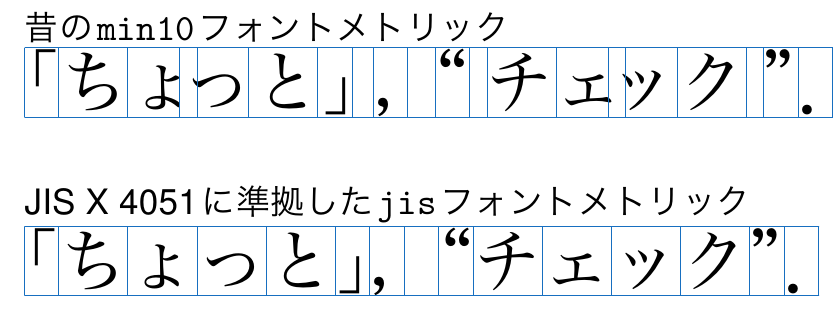
\includegraphics[width=.4\linewidth]{./image2012-gum/Okumura2011.png}
  \caption{日本語組版の例。上が{\pLaTeX}を用いた場合。下が奥村さんの新ドキュメントクラスを用いた場合(奥村, 2011)。}
  \label{fig:jisx0451}
  \vspace{-1em}
\end{figure}
句読点や括弧の処理が細かく調整されている様子が見てとれます。

最後に Unicode 対応について。
先ずお断りとして、{\TeX}における多言語処理についてはここでは割愛します\footnote{
  興味のある方は以下の URL を参照して下さい\\
  「pTeXと多言語処理」{\tt{\url{http://oku.edu.mie-u.ac.jp/~okumura/texwiki/?pTeX\%E3\%81\%A8\%E5\%A4\%9A\%E8\%A8\%80\%E8\%AA\%9E\%E5\%87\%A6\%E7\%90\%86}}}
}。
%
「ファイルの文字コードとして UTF-8 を使いたい」つまり「多言語混在の UTF-8 のファイルを直接処理したい」という
場合にも、最新の{\pLaTeX}(正確には $\varepsilon-$拡張がなされた $\varepsilon-$\pTeX)であれば、
そのまま処理できます。つまり、次の安定版(Wheezy)では、UTF-8 で保存されたソースをそのまま \pLaTeX で処理できるようになる……はずです%
(残念ながら squeeze では処理できません)。

\subsubsection{世界情勢}

ここで一端日本語を離れて、
日本語以外の{\TeX}(とその拡張)および多言語処理がどの様に発展しているのか、について簡単に触れてみましょう。
%
Knuthさんの{\TeX}開発終了宣言の後でも、
最下層の処理系としての{\TeX}は進化を続けており、$\varepsilon-$\TeX、そして pdf\TeX へと進展しています。
現在では{\LaTeX}として{pdf\LaTeX}が使われるのが一般的です
% \footnote{%%
%   お手元の環境で{\tt{latex}}と打ってみて下さい。おそらくエンジンとして{\tt{pdftex}}が起動するでしょう。
% }
。
pdf{\TeX}はその名の通り DVI ファイルを経ずに直接 PDF ファイルを出力する{\TeX}エンジンです。
この結果として、今後は DVI ファイルは過去の遺物になっていくのかもしれません
\footnote{
  これは日本語処理としてはある意味ありがたい話です。
  DVIファイルにはフォントの「参照」しか表れないため、表示が環境によって異なり、DeVice Independent が実現されません。
  PDF の場合はどうか、といえば、そもそも欧文のPDFの場合にはフォントを埋め込むのが一般的であり、
  和文のみが参照名({\tt{Ryumin-Light, GothicBBB-Medium}})のみで実フォントは埋め込まない、という状況でした。
  しかしながら、
  JIS2004前後で同じコードポイントに別のグリフが割り当てられているため、
  フォントを埋め込んでいない PDF では表示が異なる、という問題が発生します。
  %
  今後は欧文和文区別なく、フォントを埋め込んだ PDF を出力する、というのが一般的になるでしょう。
}
。
また、$\varepsilon-$\TeX は元々の \TeX に対して多くの拡張がなされています。
現在既に多くの拡張機能が$\varepsilon-${\TeX}に依存しているため、
$\varepsilon-${\TeX}に対応していないエンジンは時代遅れになりかねません%
\footnote{%
  幸いな事に北川弘典さんを中心に$\varepsilon-$\pTeX(=\pTeX + $\varepsilon-$TeX)が公開されており、
  TeXLive 本体にも同梱されています。本原稿執筆時点では既に
  Debian unstable で日本語環境を導入すると \pLaTeX のエンジンとして $\varepsilon-$\pTeX が使われています。
}

多言語処理系としては、壮大な試みであった$\Omega$が頓挫(?)した後、
現在ではXeTeX(=$\varepsilon-$\TeX + Unicode + OpenType) を用いるのが一般的になってきました。
Unicode での入出力を処理し、システムのフォントを利用して直接 PDF を出力します。
%
また、pdf{\TeX}の後継としてLua{\TeX}(pdf\TeX + $\Omega$ + Lua + METAPOST + OpenType)の開発が進められています。
Lua による柔軟な拡張が可能となっており、今後の進展が楽しみではあります。

なお、現時点では Xe(La)TeX および LuaTeX を用いて、
JIS X 4051 で規定された日本語の組版を実現するためには別パッケージが必要だったり、
プリアンブルをそれなりに修正する必要があるので一筋縄ではいきません。
%
今後に備えて動向を確認しておくのも良いでしょう
\footnote{
  \noindent
  XeTeX に関しては「XeLaTeXで日本語する件について」{\tt{\url{http://zrbabbler.sp.land.to/xelatex.html}}} \\
  LuaTeX-ja に関しては「LuaTeX-ja プロジェクト」{\tt{\url{http://sourceforge.jp/projects/luatex-ja/wiki/FrontPage}}}
}。

\subsubsection{{\TeX}Live について}

最後に、{\TeX}Liveについて。
{\TeX}に関するソフトウェアを提供する「ディストリビューション」として、以前は te\TeX がリリースされていました。
しかしながら、2009年に te\TeX としてリリースを停止した後\footnote{%
   teTeX: no next release
   「{\tt{\url{http://article.gmane.org/gmane.comp.tex.tetex.beta/812}}}」
}、
{\TeX}Live が{\TeX}のディストリビューションとしてリリースされるようになりました。
%
{\TeX}Live のリリースマネージャは Norbert Preining さんで、
彼は Debian の {\TeX} 関連パッケージのメンテナでもあります。
{\TeX}Live では {\tt{tpm2deb}} や {\tt{tpm2rpm}} といったパッケージ変換スクリプトも提供されており、
現在では多くの Linux ディストリビュータが {\TeX}Live を元に各々のパッケージを作成しています。
%
日本語関連については、2010年以降に {\TeX}Live本体への \pTeX、j{\TeX} のマージが開始され、
本原稿執筆時点では、patch の著作権者にコンタクトの取れていない {\tt{xdvik-ja}} 以外は
ほぼマージが完了しています。

\subsection{Debianにおける(日本語){\TeX}環境}

さてここまでのお話を踏まえた上で、ようやく Debian の{\TeX}環境について触れていきます。
%
ちなみに、「Debianでの{\pLaTeX}の設定」みたいな話はぐぐると結構でてくるので、あまり触れません
\footnote{%
  発表時および発表後は Q\&A および設定のお手伝いは行ないます。
}。

\subsubsection{Squeeze における(日本語){\TeX}環境}

Squeeze にて配布されている {\TeX}Live のバージョンは 2009 です。
ですので \pTeX および j{\TeX} 関連は、
$\varepsilon-$\TeX 拡張前の{\bf{UTF-8}}
のファイルを処理できないバージョンです。
具体的には、{\tt{ptex-buildsupport}} パッケージで te{\TeX}のソースを提供し、
これに patch を当てることで \pTeX や j{\TeX} のパッケージが構築されています。
%
また、ベースとなっているte{\TeX}のバージョンも 2007 であり、
セキュリティフィックスはなされているものの、
大雑把に言えば{\bf{2007年から更新されていません}}\footnote{%
  Squeeze リリース前に xdvik-ja の 64bit 対応の必要があり、
  佐々木が patch を当ててパッケージを再構築したりしました。
}。

導入後にも、
DVI ファイルの表示や PostScript/PDF への変換のために
幾つかおまじないが必要だったりします。
%
例えば
\begin{enumerate}
\item dvipsk-ja 用の VF ファイルの準備のために、インストール後に以下を唱える。
  \begin{commandline}
    $ sudo jisftconfig add
  \end{commandline}
  % $
\item xdvik-ja での表示のために
  \begin{commandline}
    # 明朝系の表示に使用するフォント
    $ fc-match serif:lang=ja
    # ゴシック系の表示に使用するフォント
    $ fc-match sans-serif:lang=ja
  \end{commandline}
  \noindent を確認し
  % \footnote{%
  %   {\tt{ttf-tamil-fonts}} や
  %   {\tt{ttf-devanagari-fonts}} がインストールされている場合には、
  %   これらが返ってきてしまい、
  %   結果として DVI の表示にこれらのフォントが使われる。
  % }
  、
  必要に応じて、{\tt{$\tilde{}$/.fonts.conf}} に
  {\tt{serif, sans-serif}}のエントリを追記して
  \begin{commandline}
    $ sudo update-vfontmap
  \end{commandline}
  % $
\item フォントが埋め込まれていない
  PDF の表示のために、{\tt{Ryumin, Gothic-BBB}}のエントリを
  {\tt{$\tilde{}$/.fonts.conf}}に追記する。
\item フォントを埋め込んだ PDF を生成するためには、
  {\tt{/etc/texmf/texmf.d/75DviPS.cnf}} の {\tt{TTFONTS}}、
  もしくは{\tt{\%OSFONTDIR}} に埋め込みたいフォントのパスを追加した後に
  \begin{commandline}
    $ sudo update-texmf
  \end{commandline}
  % $
  を唱えて、さらに map ファイルを適当に用意しておく。
\end{enumerate}
\vspace{-.8em}
などです。

\subsubsection{Squeezeで{\tt{{\TeX}Live(>=2011)}}を使う!?}

Debianのパッケージではありませんが、amd64 もしくは i386 の場合には
Norbert さんを中心に提供されている「tlptexlive リポジトリ\footnote{
  tlptexlive リポジトリ「{\tt{\url{http://tutimura.ath.cx/ptexlive/?tlptexlive\%A5\%EA\%A5\%DD\%A5\%B8\%A5\%C8\%A5\%EA}}}」
}」から、
TeXLive 全体のコンパイル済みバイナリを取得して使用する、という方法もあります。
%
この場合には
\begin{enumerate}
\item 既存の Debian パッケージの依存関係解消のために {\tt{equivs}} でダミーパッケージを作成する
\item {\TeX}Live のパッケージマネージャである{\tt{tlmpgr}}でのバイナリ導入先を、
  管理しやすい所に追いておく。
\end{enumerate}
なんて工夫が必要でしょう。佐々木は Squeeze 環境で
は {\tt{stow}} で tlptexlive リポジトリでのインストール物を管理しています。

ちなみに tlptexlive の配布物は {\tt{{\TeX}Live (>= 2011)}} 相当ですので、
フォント周りの設定は後述の Wheezy の場合と同じです。

\subsubsection{Wheezy の現状}

既に{\TeX}Live 2011(2012/dev) が Sid に upload されています。しかしながら、
本原稿執筆時点ではまだ Wheezy には更新された{\TeX}関連のパッケージは落ち
てきていません。
発表時には Wheezy に落ちてきていることを期待しつつ、
変更点を簡単に述べてみます。

このバージョンの {\TeX}Live には既に\pTeX などがマージされているため、
Squeeze までで提供していた te\TeX ベースのパッケージ群{\tt{ptex-bin, ptex-base, ...}}は軒並 obsolete となります\footnote{%
  {\TeX}Live 本体にマージされていない{\tt{xdvik-ja}}のみが残ることになります。
}。
%
現状では \pTeX 関連は {\tt{texlive-binaries, texlive-lang-cjk}} を導入することで一括で install される予定です。
また、フォント関連の扱いも {\tt{updmap-setup-kanji}} というコマンドによって、一括で設定できるようになります。
%
たとえば
\begin{commandline}
  $ sudo updmap-setup-kanji nofont
\end{commandline}
%$
\noindent といった塩梅です(上記の設定は、フォントをまったく埋め込まない場合です)。
このコマンドにより、{\tt{xdvik-ja, dvips, dvipdfmx}} のフォントマップが一括して更新されます。
%
{\TeX}Live ではフォントマップファイルとして、
1)埋め込まない場合、 2)IPAex を使う場合、3)ヒラギノを使う場合、4)小塚フォントを使う場合
の 4 つを提供しており、Debian のパッケージでもこれらのマップファイルを提供しています。
Debian の main セクションのみで作業をする場合には 1) or 2) を使うことになるでしょう。
現時点では、
\begin{itemize}
\item Conflicts, Replace, Provides の設定が半端で
  Squeeze からの upgrade がうまくできない(パッケージがある)。
\item {\TeX}Live 本体でも配布されているフォントがあり、
  既存のパッケージと重複しているため、Depends を追加して適宜 symbolic link に
  置換する必要がある。
\end{itemize}
といった問題があって、今後の修正が大変ですが、
Wheezy のリリースまでにはちゃんと直る(直す?)でしょう。

\subsection{最後に}

駆け足でしたが、日本語{\TeX}の現状および
Debian での{\TeX}関連の現状をまとめてみました。
%
まだまだ修正すべき点もありますが、
今後は{\tt{updmap-setup-kanji}}によるフォント関連の一括管理が有効になるため、
おまじないのような、
ともすればバッドノウハウと扱われがちな煩雑な設定は不要になるでしょう。
%
Wheezy からは、UTF-8 へ対応した \pTeX が、
もっと言えばJIX X 4051の組版要件を満たしつつ多言語処理も可能となった
日本語{\TeX}環境が非常に簡単に手に入るようになる予定です\footnote{%
  本来であればここで参考文献を列記すべきですが、
  紙面の都合上脚注に記す無作法をお許し下さい。
}。



%------------------------------------------------------------------------------
\dancersection{Linux-PAMの設定について}{西山和広}
\label{linux-pam}
\subsection{Introduction}
\label{sec-1-1}
\subsubsection{PAM とは何か?}
\label{sec-1-1-1}
%------------------------------------------------------------------------------

Linux-PAM (Pluggable Authentication Modules for Linux) とは、アプリケーションがユーザーをどう認証するかをローカルシステムの管理者が設定できるようにするための共有ライブラリ一式です。

PAM のおかげで、アプリケーションをコンパイルしなおさなくても、認証方法を変更したり、権限の付与の仕方を変更したりできるようになっています。
\subsubsection{NSS とは何か?}
\label{sec-1-1-2}

PAM と関係の深いライブラリとして NSS (Name Service Switch) があります。
NSS はユーザー名とユーザー ID との変換をしたり、ホスト名と IP アドレスとの変換をしたりするときに使われます。
\subsubsection{PAM と NSS との違い}
\label{sec-1-1-3}

PAM は認証部分のみなので、基本的にはログインやログアウトのときとパスワード変更に関係します。 (厳密にはアプリケーション次第です。)

ログイン中に \verb~id~ コマンドで表示されるユーザーIDとユーザー名の対応 \footnote{グループIDとグループ名も同様です。 } や \verb~ls -l~ でファイルシステムに記録されているユーザーIDからユーザー名への変換 \footnote{ファイルシステムには所有者はユーザーIDで記録されています。そのため、たとえばユーザーを削除して存在しないユーザーのファイルがある場合には、ユーザー名への変換が出来ないので数字で表示されます。 } などは \verb~/etc/nsswitch.conf~ で設定する NSS の機能になります。
\subsubsection{PAM の設定}
\label{sec-1-1-4}

PAM は設定ファイルに実行したいモジュールを並べておいて、それを順番に実行していくようなものだと思えば良いでしょう。

たとえば、
\begin{itemize}
\item \verb~/etc/passwd~ などのローカルファイルでの認証
\begin{itemize}
\item 成功すれば認証成功をアプリケーションに返す
\item 失敗すれば次へ
\end{itemize}
\item LDAP での認証
\begin{itemize}
\item 成功すれば認証成功をアプリケーションに返す
\item 失敗すれば次へ
\end{itemize}
\item 次がないので認証失敗をアプリケーションに返す
\end{itemize}
という動作をします。
\subsection{ファイル配置}
\label{sec-1-2}
\subsubsection{設定ファイル}
\label{sec-1-2-1}

\verb~/etc/pam.d/~ の下にアプリケーションごとの設定ファイルがあります。
以下はその例です。


\begin{commandline}
$ ls /etc/pam.d
atd       chsh            common-password                cron      other   su
chfn      common-account  common-session                 login     passwd  sudo
chpasswd  common-auth     common-session-noninteractive  newusers  sshd
\end{commandline}
%$

\begin{itemize}
\item どの設定ファイルがどのアプリケーションのものなのかはファイル名から推測できます
\item ない場合は \verb~other~ が使われます
\item それぞれの中から \verb~@include~ で \verb~common-*~ で共通の設定を使うようになっています
\end{itemize}

\verb~/etc/pam.d/~ がない場合は \verb~/etc/pam.conf~ が使われると \verb~/etc/pam.conf~ の中のコメントに書いてありますが、この記述は歴史的なもので最近の Linux では使われていません。
\subsubsection{モジュール}
\label{sec-1-2-2}

以下は PAM モジュールの例です。


\begin{commandline}
$ ls /lib/x86_64-linux-gnu/security
pam_access.so     pam_keyinit.so    pam_nologin.so     pam_tally.so
pam_debug.so      pam_lastlog.so    pam_permit.so      pam_tally2.so
pam_deny.so       pam_ldap.so       pam_pwhistory.so   pam_time.so
pam_echo.so       pam_limits.so     pam_rhosts.so      pam_timestamp.so
pam_env.so        pam_listfile.so   pam_rootok.so      pam_umask.so
pam_exec.so       pam_localuser.so  pam_securetty.so   pam_unix.so
pam_faildelay.so  pam_loginuid.so   pam_selinux.so     pam_userdb.so
pam_filter.so     pam_mail.so       pam_sepermit.so    pam_warn.so
pam_ftp.so        pam_mkhomedir.so  pam_shells.so      pam_wheel.so
pam_group.so      pam_motd.so       pam_stress.so      pam_xauth.so
pam_issue.so      pam_namespace.so  pam_succeed_if.so
\end{commandline}
%$

\begin{itemize}
\item 設定ファイルに書かれる \verb~pam_unix.so~ などは \verb~dlopen(3)~ で動的に読み込まれます
\item そのため PAM の認証を使っているプログラムを入れた chroot 環境を作るときには気をつける必要があります
\item \verb~squeeze~ までは \verb~/lib/security/~ や \verb~/lib64/security/~ にあります
\item \verb~multiarch~ 対応で最近は \verb~/lib/x86_64-linux-gnu/security/~ などの \verb~/lib/<triplet>/security/~ にあります。
  上記の例は wheezy (testing) なので \verb~/lib/security/~ ではなく
  \verb~/lib/x86_64-linux-gnu/security/~ になっています
\end{itemize}
\subsection{設定ファイルの書式}
\label{sec-1-3}

設定ファイルの例を載せておきます。(一部省略)

\begin{commandline}
$ egrep '^[^#]' /etc/pam.d/cron
@include common-auth
session       required   pam_env.so
session       required   pam_env.so envfile=/etc/default/locale
@include common-account
@include common-session-noninteractive
session    required   pam_limits.so
\end{commandline}
%$

\begin{itemize}
\item 設定ファイルには以下の項目を指定します。詳細は後述します
\begin{description}
\item[\verb~service~] アプリケーションに対応する名前
\item[\verb~type~] PAM の分類
\item[\verb~control~] 動作指定
\item[\verb~modules-path~] PAM モジュールへのパス
\item[\verb~module-arguments~] PAM モジュールの引数
\end{description}
\item \verb~#~ から行末まではコメントになります
\item \verb~\~ が改行 (\verb~<LF>~) の直前にあると継続行になります
\item \verb~/etc/pam.conf~ では「 \verb~service type control module-path module-arguments~ 」という書式で設定します。( \verb~service~, \verb~type~, \verb~control~ の大文字小文字は無視されます。)
\item \verb~/etc/pam.d/~ では \verb~service~ がファイル名 (必ず小文字) になります
\item 残りの「 \verb~type control module-path module-arguments~ 」がファイルの内容になります
\end{itemize}
\subsubsection{service}
\label{sec-1-3-1}

\begin{itemize}
\item \verb~service~ は具体的には \verb~login~ や \verb~su~ になります
\item \verb~other~ という \verb~service~ 名はデフォルト設定用として予約されています
\item Debian では \verb~common-~ で始まる名前のファイルが共通設定用のファイルになっていて、他の設定ファイルから \verb~@include~ で読み込まれています
\end{itemize}
\subsubsection{type}
\label{sec-1-3-2}

\begin{description}
\item[account] 認証以外のアカウント管理に使われます。たとえば昼間だけログインできるようにしたり、 \verb~nologin~ ファイルがあるときは一般ユーザーにログインさせないようにしたりできます
\item[auth] アプリケーションにパスワード入力を要求するなどの方法でユーザー認証をします。グループ権限の付与などの機能もあります
\item[password] パスワード変更などの認証トークン変更機能を提供します
\item[session] サービス利用の前後に何かをするモジュールタイプです。ログを取ったり、ディレクトリをマウントしたり、 \verb~/etc/motd~ を表示したり、環境変数を設定したりできます
\item[\verb~@include~] Debian ではここに \verb~@include~ を指定することで別のファイルを読み込めるようになっています
\end{description}
\subsubsection{control}
\label{sec-1-3-3}

PAM モジュールを実行してその結果、どうするのかの設定です。
詳細については後述します。
\subsubsection{module-path}
\label{sec-1-3-4}

PAM モジュールのファイルへのパスを絶対パスかデフォルトのモジュールの置き場所である \verb~/lib/security/~ などからの相対パスで指定します。
\subsubsection{module-arguments}
\label{sec-1-3-5}

スペース区切りでモジュールへの引数を指定します。
スペースを含む引数を指定する場合は以下の例のように \verb~[]~ でくくります。


\begin{commandline}
squid auth required pam_mysql.so user=passwd_query passwd=mada \
      db=eminence [query=select user_name from internet_service \
      where user_name='%u' and password=PASSWORD('%p') and \
      service='web_proxy']
\end{commandline}

\verb~]~ を含めたい場合は \verb~\]~ と指定します。
つまり以下のようになります。


\begin{commandline}
[..[..\]..]    -->   ..[..]..
\end{commandline}
\subsection{control の設定について}
\label{sec-1-4}
\subsubsection{PAM の内部状態}
\label{sec-1-4-1}

PAM はモジュールを実行していくときに内部的に
\begin{itemize}
\item 初期状態
\item 成功状態
\item 失敗状態
\end{itemize}
の3つの状態があり、最終的に成功状態なら成功をアプリケーションに返し、そうでなければ失敗をアプリケーションに返します。
(初期状態のままのときも失敗を返します。)
\subsubsection{control の省略形式}
\label{sec-1-4-2}

control の指定には、省略した形式として以下のものがあります。

\begin{description}
\item[required] 成功しても失敗しても続きを実行してから結果を返します。失敗状態以外で成功した場合は成功状態にします。失敗した場合は失敗状態にします
\item[requisite] 失敗した場合は失敗状態にして、すぐにアプリケーションに失敗を返します。失敗状態以外で成功した場合は成功状態にします
\item[sufficient] 失敗状態以外で成功した場合は、すぐにアプリケーションに成功を返します。失敗は無視して続きを実行します
\item[optional] 成功か失敗かは気にせず実行したいモジュールに使います。成功か失敗かは他のモジュールがないときだけ影響します
\item[include, substack] 省略形式ではありませんが、このような指定も出来ます。しかし Debian では上述の \verb~@include~ が使われていて、これらは普通は使われていないのと、内部状態の説明が複雑になるため省略します
\end{description}
\subsubsection{control の省略しない形式}
\label{sec-1-4-3}

もっと複雑な形式として以下のものがあります。


\begin{commandline}
[value1=action1 value2=action2 ...]
\end{commandline}
\subsubsection{control の value}
\label{sec-1-4-4}

\verb~valueN~ は PAM モジュールからの返値で \verb~actionN~ はその返値のときにどうするかという設定です。
\verb~valueN~ には、

{\scriptsize
\begin{tabular}{cc}
  \begin{minipage}[b]{0.3\textwidth}
    \begin{itemize}
    \item \verb~success~
    \item \verb~open_err~
    \item \verb~symbol_err~
    \item \verb~service_err~
    \item \verb~system_err~
    \item \verb~buf_err~
    \item \verb~perm_denied~
    \item \verb~auth_err~
    \item \verb~cred_insufficient~
    \item \verb~authinfo_unavail~
    \item \verb~user_unknown~
    \end{itemize}
  \end{minipage}
  \begin{minipage}[b]{0.3\textwidth}
    \begin{itemize}
    \item \verb~maxtries~
    \item \verb~new_authtok_reqd~
    \item \verb~acct_expired~
    \item \verb~session_err~
    \item \verb~cred_unavail~
    \item \verb~cred_expired~
    \item \verb~cred_err~
    \item \verb~no_module_data~
    \item \verb~conv_err~
    \item \verb~authtok_err~
    \item \verb~authtok_recover_err~
    \end{itemize}
  \end{minipage}
  \begin{minipage}[b]{0.3\textwidth}
    \begin{itemize}
    \item \verb~authtok_lock_busy~
    \item \verb~authtok_disable_aging~
    \item \verb~try_again~
    \item \verb~ignore~
    \item \verb~abort~
    \item \verb~authtok_expired~
    \item \verb~module_unknown~
    \item \verb~bad_item~
    \item \verb~conv_again~
    \item \verb~incomplete~
    \item \verb~default~
    \end{itemize}
  \end{minipage}
\end{tabular}
}

が指定できます。
\verb~default~ は名前からわかる通り明示的に \verb~valueN~ に指定されなかったときのデフォルト指定です。

\verb~valueN~ に指定できる値の完全なリストは \verb~libpam0g-dev~ パッケージをインストールして
\begin{itemize}
\item \verb~/usr/include/security/_pam_types.h~
\end{itemize}
を参照してください。
\subsubsection{control の action}
\label{sec-1-4-5}

\verb~actionN~ に指定できるものは以下の通りです。

\begin{description}
\item[ignore] 無視します。モジュールの返値はアプリケーションに返す値には影響しません
\item[bad] 失敗状態にします
\item[die] 失敗します。失敗状態にして、すぐにアプリケーションに失敗を返します
\item[ok] 失敗状態以外なら成功状態にします。すでに失敗状態のときは失敗状態のままです
\item[done] 失敗状態以外なら成功状態にして、すぐにアプリケーションに成功を返します。すでに失敗状態のときは失敗状態のままです
\item[N (1以上の整数)] 次の N 個のモジュールを実行せずに飛ばします
\item[reset] 内部状態を初期状態に戻します
\end{description}
\subsubsection{省略形の展開}
\label{sec-1-4-6}

省略形は \verb~[...]~ の書式で書くと以下のようになります。

\begin{description}
\item[required] \verb~[success=ok new_authtok_reqd=ok ignore=ignore default=bad]~
\item[requisite] \verb~[success=ok new_authtok_reqd=ok ignore=ignore default=die]~
\item[sufficient] \verb~[success=done new_authtok_reqd=done default=ignore]~
\item[optional] \verb~[success=ok new_authtok_reqd=ok default=ignore]~
\end{description}
\subsection{PAM 設定フレームワーク}
\label{sec-1-5}

Red Hat 系 Linux には以前から PAM や NSS の自動設定用のコマンドとして \verb~authconfig~ があります。
しかし、昔の Debian にはそういうフレームワークはありませんでした。

Ubuntu では、そのようなフレームワークとして \verb~auth-client-config~ が使われるようになりました。
その後 \verb~pam-auth-update~ が使われるように変わりました。
そして Debian にも \verb~pam-auth-update~ が入って今は Debian でも Ubuntu でも \verb~pam-auth-update~ が標準の PAM の設定用フレームワークとして使われています。\footnote{Debian にはありませんが、 Ubuntu には \verb~auth-client-config~ パッケージはまだ存在しています。 \verb~pam-auth-update~ は PAM の設定のみなので、もしかすると NSS の設定には使われているのかもしれません。(使っていないので詳細は不明です。) }
\subsubsection{pam-auth-update}
\label{sec-1-5-1}

\verb~pam-auth-update~ コマンドは \verb~libpam-runtime~ パッケージに入っています。
PAM モジュールパッケージで \verb~/usr/share/pam-configs~ の中にプロファイルがインストールされます。
\verb~pam-auth-update~ コマンドは、そのプロファイルを元に \verb~/etc/pam.d/common-*~ ファイルを更新します。
\subsection{設定ファイルの例}
\label{sec-1-6}

\begin{itemize}
\item \verb~pam-auth-update~ で生成された設定ファイルの一部と sshd の設定を例として説明をします。
\end{itemize}
\subsubsection{/etc/pam.d/common-auth}
\label{sec-1-6-1}

common-auth は認証の共通処理の設定ファイルです。
\begin{enumerate}
\item まず最初に ``Primary'' block のモジュールを \verb~pam_unix.so~, \verb~pam_ldap.so~ と順番に試して、どこかで成功したら \verb~pam_permit.so~ まで飛ばして成功状態にします
\item すべて失敗した場合は fallback の \verb~pam_deny.so~ の行で必ず失敗して、そのままアプリケーションに認証失敗を返します
\item 途中で成功して \verb~pam_permit.so~ の行に飛んできた場合は、そのまま続きの行を実行していきます
\item \verb~@include~ 元のファイルで続きの処理を用意していることもあるので \verb~sufficient~ で成功をすぐに返してしまうことは避けて \verb~success=N~ で飛ばして \verb~pam_permit.so~ で成功状態にするという手間をかけているようです
\item \verb~pam_ldap.so~ の \verb~use_first_pass~ は \verb~pam_unix.so~ の認証のときに入力されたパスワードを使って \verb~pam_ldap.so~ の認証も試すという意味です。 \verb~use_first_pass~ がないと \verb~pam_unix.so~ でパスワード入力が要求されて、さらに \verb~pam_ldap.so~ でもパスワード入力を要求されるということになります。(プロファイルで Auth-Initial と Auth にわかれているのはそういう設定を使いわけられるようにするためのようです。)
\end{enumerate}

\begin{commandline}
# here are the per-package modules (the "Primary" block)
auth    [success=2 default=ignore]      pam_unix.so nullok_secure
auth    [success=1 default=ignore]      pam_ldap.so minimum_uid=1000 use_first_pass
# here's the fallback if no module succeeds
auth    requisite                       pam_deny.so
# prime the stack with a positive return value if there isn't one already;
# this avoids us returning an error just because nothing sets a success code
# since the modules above will each just jump around
auth    required                        pam_permit.so
# and here are more per-package modules (the "Additional" block)
auth    optional                        pam_cap.so
# end of pam-auth-update config
\end{commandline}
\subsubsection{/etc/pam.d/common-session}
\label{sec-1-6-2}

\begin{itemize}
\item この例の common-session では ``Primary'' block にモジュールがないために \verb~pam_permit.so~ でいきなり \verb~pam_deny.so~ を飛びこえるようになっています
\item その後 \verb~pam_unix.so~ と \verb~pam_ldap.so~ でも何か追加の処理をして \verb~pam_tmpdir.so~ で環境変数 TMPDIR などを設定しています
\end{itemize}

\begin{commandline}
# here are the per-package modules (the "Primary" block)
session [default=1]                     pam_permit.so
# here's the fallback if no module succeeds
session requisite                       pam_deny.so
# prime the stack with a positive return value if there isn't one already;
# this avoids us returning an error just because nothing sets a success code
# since the modules above will each just jump around
session required                        pam_permit.so
# and here are more per-package modules (the "Additional" block)
session required        pam_unix.so
session [success=ok default=ignore]     pam_ldap.so minimum_uid=1000
session optional pam_tmpdir.so
# end of pam-auth-update config
\end{commandline}
\subsubsection{/etc/pam.d/sshd}
\label{sec-1-6-3}

\begin{enumerate}
\item まず \verb~pam_env.so~ で環境変数を設定しています
\item \verb~#~ で始まる行だけでなく、行の途中の \verb~#~ 以降もコメントです
\item 2個目の \verb~pam_env.so~ で \verb~/etc/default/locale~ を読み込んでいます \footnote{余談ですが、昔の Debian では \verb~/etc/default/locale~ は存在しなくて、アップグレードでも自動で作成はされず、ログをみるとエラーが出ていたということがあり、そのときは自分で \verb~/etc/default/locale~ を作成しました。今は \verb~update-locale~ というコマンドで更新するとチェックもしてくれて良い感じになるようです。 }
\item \verb~pam_nologin.so~ では \verb~nologin~ ファイルがあるときにログインを認可しないようにしています
\item session では \verb~pam_motd.so~ で \verb~/etc/motd~ の表示をしています。最近の Debian や Ubuntu の \verb~pam_motd.so~ では \verb~/etc/update-motd.d~ があれば表示前に内容が更新されるようになっています。 Ubuntu のサーバーに ssh でログインしたときにいろいろな情報がでるのはそのためです。 Ubuntu の場合は update-notifier-common を入れておくとパッケージの更新や再起動が必要かどうかが ssh などでのログイン時に出るようになるのでおすすめです。 Debian では \verb~/etc/update-motd.d~ のファイルが入らない ( \href{http://bugs.debian.org/580286}{http://bugs.debian.org/580286} ) ため、自動では出ません
\item 他にはメールボックスの状態を表示したり、リソース制限を反映したりしているようです
\end{enumerate}

\begin{commandline}
# PAM configuration for the Secure Shell service

# Read environment variables from /etc/environment and
# /etc/security/pam_env.conf.
auth       required     pam_env.so # [1]
# In Debian 4.0 (etch), locale-related environment variables were moved to
# /etc/default/locale, so read that as well.
auth       required     pam_env.so envfile=/etc/default/locale

# Standard Un*x authentication.
@include common-auth

# Disallow non-root logins when /etc/nologin exists.
account    required     pam_nologin.so

# Uncomment and edit /etc/security/access.conf if you need to set complex
# access limits that are hard to express in sshd_config.
# account  required     pam_access.so

# Standard Un*x authorization.
@include common-account

# Standard Un*x session setup and teardown.
@include common-session

# Print the message of the day upon successful login.
session    optional     pam_motd.so # [1]

# Print the status of the user's mailbox upon successful login.
session    optional     pam_mail.so standard noenv # [1]

# Set up user limits from /etc/security/limits.conf.
session    required     pam_limits.so

# Set up SELinux capabilities (need modified pam)
# session  required     pam_selinux.so multiple

# Standard Un*x password updating.
@include common-password
\end{commandline}
\subsection{設定変更時の注意事項}
\label{sec-1-7}

設定を変更するときは root 権限のシェルを開いたままにしておくことをお勧めします。
もし設定を間違えてしまうと sudo も su もコンソールからの root でのログインも出来なくなって困ることになります。

ただし \verb~pam-auth-update~ を使ってパッケージでインストールされた設定の有効無効を切り替えるだけの場合は問題が起きる可能性は低いので、そこまでしなくても普通は大丈夫だと思います。
\subsection{参考文献}
\label{sec-1-8}

\begin{itemize}
\item \href{http://linux-pam.org/Linux-PAM-html/Linux-PAM_SAG.html}{http://linux-pam.org/Linux-PAM-html/Linux-PAM\_SAG.html} The Linux-PAM System Administrators' Guide Version 1.1.2, 31. August 2010
\item \href{http://archive.linux.or.jp/JF/JFdocs/User-Authentication-HOWTO/}{http://archive.linux.or.jp/JF/JFdocs/User-Authentication-HOWTO/} User Authentication HOWTO 2000/05/02
\item \href{https://wiki.ubuntu.com/PAMConfigFrameworkSpec}{https://wiki.ubuntu.com/PAMConfigFrameworkSpec} PAMConfigFrameworkSpec - Ubuntu Wiki
\item \href{https://wiki.ubuntu.com/AuthClientConfig}{https://wiki.ubuntu.com/AuthClientConfig} AuthClientConfig - Ubuntu Wiki
\end{itemize}


%------------------------------------------------------------------------------
\dancersection{数学ソフトウェア使ってますか?}{濱田龍義}
\label{sec:MathLibre}
%------------------------------------------------------------------------------

\vspace{2em}
% add upper space for logo

Debian パッケージには「数学」というセクションが存在し、多数の数学ソフト
ウェアが提供されています。 一方で、パッケージには未収録ですが、
数学の研究、教育の現場で使われているフリーソフトウェアが
世界中で開発されています。
2003年頃から、このような数学ソフトウェアをライブCDであるKNOPPIX に収録して紹
介してきたプロジェクトが KNOPPIX/Math です。
KNOPPIX は Debian をベースに、ドイツの Klaus Knopper によって開発が進
められている Live Linux です。当初は CD 起動のみに対応していましたが、
DVD や USB メモリーディスクにも対応し、現在も開発が進められています。
KNOPPIX/Math では、2006年から LiveDVD を採用しました。
また、2012年からは KNOPPIX 以外のシステムの利用も考慮し、
MathLibreとプロジェクト名を変更しています。
本講演では MathLibre に収録している様々な数学ソフトウェアから、
いくつかを紹介します。

\subsection{数学ソフトウェアの歴史}
我々は、数学を取り扱うもの、また、数学に関連するもの、そういったものすべ
てを数学ソフトウェアと呼んでいます。
%例えば、前の佐々木先生の講演では\TeX{}(\TeX{}Live) が取り上げられました。
Donald E. Knuth によって生み出された組版システム \TeX{}は、
数学を生業とするものにとっては、欠かせない道具であり、
これもまた、数学ソフトウェアの一種です。
一般的に、数式処理ソフトウェア、数値計算ライブラリ、可視化ツールなども
数学ソフトウェアと考えて良いでしょう。

その中で、数式処理ソフトウェアと呼ばれるソフトウェアについて紹介します。
Debian のオフィシャルパッケージの中で、比較的使いやすい物としては、
Maxima が有名です。Maxima の原型は MACSYMA と呼ばれるシステムで、
1960年代に MIT の人工知能研究グループによって開発されました。
1980年代には MACSYMA は商用ソフトウェアとしても流通していましたが、
現在の Maxima は、William Schelter によって GNU Common Lisp 上に実装され
たものを原型に2001年にGPL化され、Maxima と名称を改めて、
フリーソフトウェアとして公開されたものです。
Maximaは、方程式の求解、多項式の因数分解、初等函数の微積分、
行列計算、グラフの描画等に対応しています。中でも積分アルゴリズムの実装につ
いて評価が高いようです。

Debian 上で Maxima を起動するための命令は {\tt maxima} です。
\begin{commandline}
knoppix@Microknoppix:~$ maxima

Maxima 5.26.0 http://maxima.sourceforge.net
using Lisp GNU Common Lisp (GCL) GCL 2.6.7 (a.k.a。GCL)
Distributed under the GNU Public License。See the file COPYING.
Dedicated to the memory of William Schelter.
The function bug_report() provides bug reporting information.
(%i1) integrate(1/(x^3+1),x);
                                         2 x - 1
                       2            atan(-------)
                  log(x  - x + 1)        sqrt(3)    log(x + 1)
(%o1)           - --------------- + ------------- + ----------
                         6             sqrt(3)          3
(%i2)
\end{commandline}
%$

\subsubsection{Maximaのユーザインターフェース}
コマンドラインからの利用が一番速く手軽ですが、
一般的なグラフィカルユーザインターフェースとしては、
XMaxima ({\tt xmaxima}) や WxMaxima ({\tt wxmaxima}) が存在します。
XMaxima は Tcl/Tk, WxMaxima は WxWidget によって
実装されています。また、Emacs 用に便利なインターフェースとしては
imaxima ({\tt maxima-emacs}) が存在します。
Emacs 上で {\tt M-x imaxima} で起動すると、
数式の計算結果を \TeX{} スタイルに整形された形で出力されます。
また、少し変わったインターフェースとしては GNU TeXmacs ({\tt texmacs})と呼ばれる
科学技術計算用ワードプロセッサが存在します。
こちらも計算結果の出力を整形された形で表示することができます。

\begin{center}
\begin{figure}[ht]
\begin{minipage}[c]{8cm}
  \includegraphics[width=1\hsize]{image2012-gum/imaxima.eps}
  \caption{imaxima on Emacs}
  \label{fig:imaxima}
\end{minipage}
\begin{minipage}[c]{8cm}
  \includegraphics[width=1\hsize]{image2012-gum/texmacs.eps}
  \caption{GNU TeXmacs}
  \label{fig:texmacs}
\end{minipage}
\end{figure}
\end{center}

Maxima と同じく、長い歴史を持つ数式処理システムとしては、Reduce もよく知られ
た存在です。
Reduce もまた、1960年代に開発が始められたシステムですが、こちらは
理論物理学からの要請により開発されました。
Reduce も MACSYMA と同様に1980年代に商品化され、日本では差分方程式論、
および可積分系等の分野で多くのユーザを獲得しています。
その後、2009年に Reduce は Tony Hearn によって BSD ライセンスで公開され、
現在に至ります。
まだ、Debian オフィシャルパッケージには含まれていませんが、
getdeb ({\tt \url{http://www.getdeb.net/}})から、パッケージが入手可能です。
Reduce もまた、微分方程式の求解、積分、行列計算、グラフの描画等に対応し
ています。

Maxima も Reduce も、たいへん歴史の古いソフトウェアであり、
現在も、多くのユーザを獲得し、開発グループが日夜、
更新を続けているソフトウェアです。
その他にも、数論の PARI/GP、群論の GAP、統計計算の R、可換環論の Singular、Macaulay2等が研究ツールとして有名です。PARI/GP、GAP、R はオフィシャルパッケージに
なっていますが、Singular、Macaulay2 については、上流開発者によるパッケー
ジは提供されていますが、オフィシャルには収録されていません。

一方、日本国内における数式処理システムの開発については、
1970年代に日本電信電話会社で AL が、1980年代に
理研で GAL が開発されました。また、1980年代末に、
富士通研究所で開発された Risa/Asir は、現在、拠点を
神戸大学に移して、研究、開発が進められています。特にグレブナー基底等、
多項式の計算に特化して、高速計算が可能であり、
MathLibre プロジェクトの中心的な存在として収録されています。
ただ、Risa/Asir は富士通研究所時代のライセンスを引き継いでおり、
オープンソースソフトウェアライセンスとは
異なるライセンスで配布されています。

\subsection{最近のシステム}
ここで、最近の動きに注目して、いくつかの数学ソフトウェアを紹介します。
\subsubsection{Sage}
Sage は2005年に William Stein によって開始されたオープンソースプロジェクトです。
彼が Sage の開発を始めた背景については
``Mathematical Software and Me: A Very Personal Recollection'' \cite{stein}に
詳しく述べられています。
現在、Sage は数学者を始めとする大勢の専門家によって開発が進められていま
す。2007年にはフリーソフトウェアの賞である
Les Troph\'{e}es du Libre の科学技術部門において金賞を受賞しています。
Sage Days と呼ばれるイベントを世界各地で開催しており、開発者と
利用者からなる巨大なコミュニティが存在します。
先日、九州大学において日本で初の Sage Days が開催され、多くの
参加者を得ました。

Sage は「車輪の再発明」はしないということを掲げており、
既に実績のある Maxima や Singular、PARI/GP、GAP、R といった
数学ソフトウェアを組み合わせることで、使いやすい環境の構築を
目指しています。それぞれの数学ソフトウェアをつなぎ合わせているのは
オブジェクト指向プログラミング言語 Python です。
Python 自身もオープンソースソフトウェアですが、世界中で熱狂的な利用者、開発者を
獲得しています。その使いやすさと、多機能性から
さまざまなプロジェクトが Python で開発されています。
それまでは、数学ソフトウェアを使いこなすためには、
そのソフトウェアごとに異なるプログラミング機能を活用しなければいけなかったのですが、
Sage は Python という一般的なプログラミング言語を
用いることで、統一的なインターフェースを提供しています。また、
Python のオブジェクト指向言語としての機能を活用できる点も
魅力となっているようです。
Sage Notebook と呼ばれるユーザーインターフェースを提供しており、
Mozilla Firefox 等の
Webブラウザ上で数式処理やグラフ描画といった機能を利用することができます。

Sageについての入門書としては、Ted Kosan による ``Sage for Newbies''
\cite{newbie} が良く知られています。これは横田博史氏によって「はじめての
Sage」\cite{ponpoko}として翻訳され、MathLibre にも収録されています。
最近、韓国では大学初年級の微分積分と線形代数について Sage を用いて解説した書籍が
出版されました。

Sage は、あまりに巨大なシステムであり、更新も頻繁であるため、
現在は、Debian パッケージとして配布されていません。Linux 用には
バイナリー版が配られています。多少の時間はかかりますが、CPUごとに最適化する
ため、ソースからコンパイルすることをお勧めします。
Windows 版については、以前は仮想マシンの Ubuntu 上で起動したサーバに
Windows 上のブラウザから接続する形式だったのですが、現在は、
Fedora Core 上で起動したサーバに Fedora Core 上の Chrome を接続させる
形になったようです。

\begin{figure}[ht]
\begin{minipage}[c]{0.45\hsize}
\includegraphics[height=0.8\hsize]{image2012-gum/sage.eps}
\caption{Sage によるグラフ描画}
\label{fig:sage}
\end{minipage}
\begin{minipage}[c]{0.48\hsize}
\includegraphics[height=0.72\hsize]{image2012-gum/taylor.eps}
\caption{GeoGebra によるテイラー多項式}
\label{fig:geogebra}
\end{minipage}
\end{figure}


\subsubsection{GeoGebra}
GeoGebra はオーストリアのヨハネスケプラー大学の Markus Hohenwarter によって
始められた数学ソフトウェアプロジェクトです。
彼はザルツブルク大学の学生時代に
テキサス・インスツルメンツ社の電卓 TI-92 Plus に触れる機会を持ちました。
彼は電卓に収録されていた動的幾何ソフト Cabri Geometry
と数式処理システム Derive に刺激を受けて開発を志したということです\cite{markus}。
2001年2月に最初のプロトタイプを開発し、
2002年3月には GeoGebra の開発でコンピュータサイエンスと数学教育に関する
修士号を取得しています.
この間、GeoGebra は、各国で数多くの賞を受賞しています。
2004年から2006年にかけては数学教育に関する PhD プロジェクトとして開発が
進められ、Austiran Academy of Sciences から支援を受けて、着実にその存在
を世界中に知らしめました。
GeoGebra もまた、オープンソースソフトウェアとして公開されています。
Java の実行環境を必要としますが、Windows、MacOS X、Linux 等、計算機環境を問わ
ずに利用可能です。Debian では stable に 3.2 系が testing に 4.0 系が
収録されています。

GeoGebra は起動すると ``Dynamic Mathematics for Everyone'' というメッセージ
を表示します。日本語に訳すと「動的数学ソフトウェア」でしょうか。
これは GeoGebra が Cabri や Cinderella と言った
動的幾何学ソフトウェア(Dynamic Geometry Software)
と呼ばれるソフトウェアの影響を受けていること、
また、主要なユーザインターフェースが動的幾何学ソフトウェアとしての機能を備えていることから類推されます。
GeoGebra という名称は幾何学(Geometry)+ 代数学(Algebra)という意の造語です.開発初期の段階では GeoGebra は動的幾何学ソフトウェアとしての機能しか持ちませんでした。しかし、現在では関数入力によるグラフ描画、数式処理、スライダー、表計算機能等を備えており、幾何学ソフトウェアという枠組みだけでは語り尽くせない存在です。

メニューやヘルプ、マニュアル等の翻訳についても世界中のボランティアスタッ
フによって活発に行われており、最新の GeoGebra 4.0 では約50ヵ国語に対応しました。
日本語化については、北海道教育大学の和地輝仁氏が中心となって進めており,
国内のユーザーを増やすきっかけとなっています。
%韓国語版については、Gyeonggi-Buk Science High School の Choi Kyeong-Sik によって翻訳が進められており、Naver という韓国最大手のインターネット検索ポータルサイトに GeoGebra のコミュニティを形成し普及に努めているようです。

GeoGebra は動的幾何学ソフトウェアとしての機能と
グラフ描画ソフトの機能が連携することで使い易いインターフェースを提供しています.
また、Maxima や Reduce と連携して数式処理機能を備えているため、
微分や積分、因数分解等の基本的な演算にも対応しています。
図 \ref{fig:geogebra} のようにグラフ上の点を動的に動かしてテイラー多項式によって描かれるグラフを観察することもできます。

表計算ビューを備えたことで、統計方面についても
機能が強化されており、教材作成に威力を発揮するものと思われます。
すべての機能を述べることはできませんが、
ヘルプやさまざまなサンプル、ムービー等も豊富で、
初めての方でも使いやすい数学ソフトウェアだと思います。
どちらかと言えば、研究よりも数学教育に焦点をあてたソフトウェアですが、
その使いやすいインターフェースから構成される可視化機能は、
プレゼンテーションなどでも威力を発揮するでしょう。
次期バージョンの4.2では本格的な数式処理シェルを備え、
5.0では3Dに対応する予定です。
潜在的な能力も含めて今後の展開が楽しみな数学ソフトウェアです。

2012年7月4日--6日にはRIMS共同研究「数式処理研究の新たな発展」が
計画されていますが、7月5日に GeoGebra Institute から
Zsolt Lavizca, Bal\'azs Koren の2人が GeoGebra の最新事情についての講演
が行われます。

\subsection{まとめ}
ここに紹介したソフトウェアは、MathLibre に収録している100以上の
数学ソフトウェアのごく一部です。本稿が、数学ソフトウェアに
興味を持っていただくきっかけになれば幸いです。

\begin{thebibliography}{99}
%\bibitem{stein1}
%David Joyner and William Stein,
%\emph{Open source mathematical software},
%Notices of the AMS、\textbf{54} (3) (2007),
%http://www.ams.org/notices/200710/tx071001279p.pdf

\bibitem{stein}
William Stein,
``\emph{Mathematical software and me:A very personal recollection}'',
\url{http://wstein.org/}

\bibitem{newbie}
Ted Kosan,
``\emph{Sage for newbies}'',
\url{http://sage.math.washington.edu/home/tkosan/}

\bibitem{ponpoko}
Ted Kosan, 横田博史 訳,
「\emph{はじめてのSage}」,
\url{http://www.bekkoame.ne.jp/~ponpoko/KNOPPIX/}

\bibitem{markus}
Markus Hohenwarter and Judith Preiner,
``\emph{Dynamic Mathematics with GeoGebra}'',
The Journal of Online Mathematics and Its Applications,
\textbf(7), 2007, \url{http://mathdl.maa.org/mathDL/}
\end{thebibliography}



%------------------------------------------------------------------------------
\dancersection{IPython notebookとその周辺}{本庄弘典}
\label{sec:ipython-notebook}
%------------------------------------------------------------------------------

\subsection{はじめに}

最近ipythonのqtconsoleでコンソール上にグラフを描画しているスクリーンショットを見る機会があり、
ちょっとかっこいいかなとロクに使ったことがないPythonを使い始めました。
今回はipython qtconsoleを使用したグラフの描画から、
Mathmatica notebooksのようなWebベースの数式処理システムipython notebookをPython初心者の視点で紹介してみたいと思います。

\subsection{IPython}

ipythonはFernando Perez氏によって作成されたPythonのインタラクティブシェルで、
現在の最新リリースバージョンは0.12.1です。
Pythonはそれ自体でインタラクティブシェルの機能を持っていますが、
ipythonはPythonシェルと比較して次の特徴を持っています。

\begin{itemize}
 \item terminalでの使用に加えQt等を用いたグラフィカルなコンソールが使用可能
 \item コード補完
 \item シンタックスハイライト
 \item 並列コンピューティングが可能
 \item Webベースのnotebook(ipython 0.12から)
\end{itemize}

Pythonシェルとipythonは次の図のように、
プロンプト等に違いがあります。

\begin{figure*}[b]
  \begin{tabular}{cc}
    \begin{minipage}[b]{0.5\textwidth}
      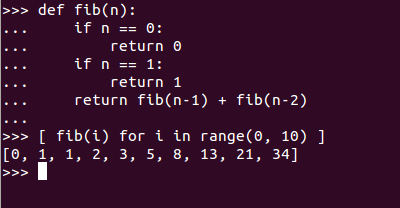
\includegraphics[width=1.0\hsize]{image2012-gum/ipython-pythonshell.png}
      \subfigure{pythonシェル}
      \label{pythonshell}
    \end{minipage}
    \begin{minipage}[b]{0.5\textwidth}
      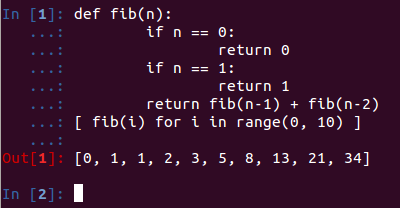
\includegraphics[width=1.0\hsize]{image2012-gum/ipython-terminal.png}
      \subfigure{ipython}
      \label{ipython}
    \end{minipage}
  \end{tabular}
  \caption{pythonシェルとipythonの違い}
\end{figure*}

\subsection{IPython qtconsole}

ipythopnにqtconsoleオプションを指定して実行することにより、
GUI環境でのipythonが起動します。
またこの環境で \texttt{--pylab inline} を指定して起動することで、
コンソール内にグラフを表示させることが可能となります。

\begin{commandline}
$ ipython qtconsole --pylab matplotlib
\end{commandline}

この環境では前述のグラフ表示に加え、
複数行をまとめて扱うコマンドの履歴などが使用できます。
グラフを描画すると次のように表示されます。

\begin{figure}[ht]
  \begin{center}
    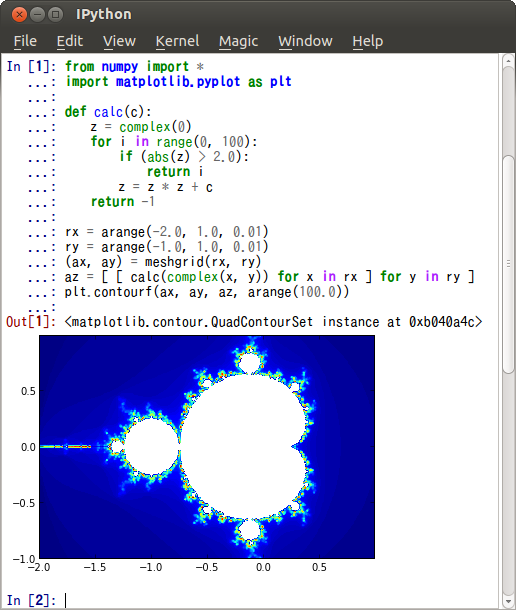
\includegraphics[width=0.6\hsize]{image2012-gum/ipython-mandelbrotset.png}
  \end{center}
  \caption{qtconsoleでマンデルブロ集合}
  \label{fig:ipython-qtconsole}
\end{figure}

testingでのipython qtconsoleおよびmatplotlibは次のコマンドでインストール出来ます。

\begin{commandline}
$ sudo aptitude install ipython-qtconsole python-matplotlib
\end{commandline}

またsqueezeはbackportsを使用してインストールを行いました。
まず/etc/apt/sources.listに次の行を追加し、

\begin{commandline}
deb http://backports.debian.org/debian-backports squeeze-backports main
\end{commandline}

\texttt{aptitude update \&\& aptitude upgrade}を実行した後、
次のコマンドでインストールします。

\begin{commandline}
$ sudo aptitude install python-setuptools python2.6-dev ncurses-dev \
  libzmq-dev python-pygments python-matplotlib pyqt4-dev-tools
\end{commandline}

パッケージのインストール後、
pythonの\texttt{easy\_install}コマンドを使用してipythonをインストールします。

\begin{commandline}
$ sudo easy_install readline pyzmq ipython
\end{commandline}

\subsection{IPython notebook}

ipython notebookはWebベースの数式処理システムで、
次の機能を備えています。

\begin{itemize}
 \item Pythonコードの実行と結果の表示
 \item Markdownによるマークアップ可能なノート
 \item MathJaxによる \TeX 形式での数式の記述
\end{itemize}

\begin{figure}[ht]
  \begin{center}
    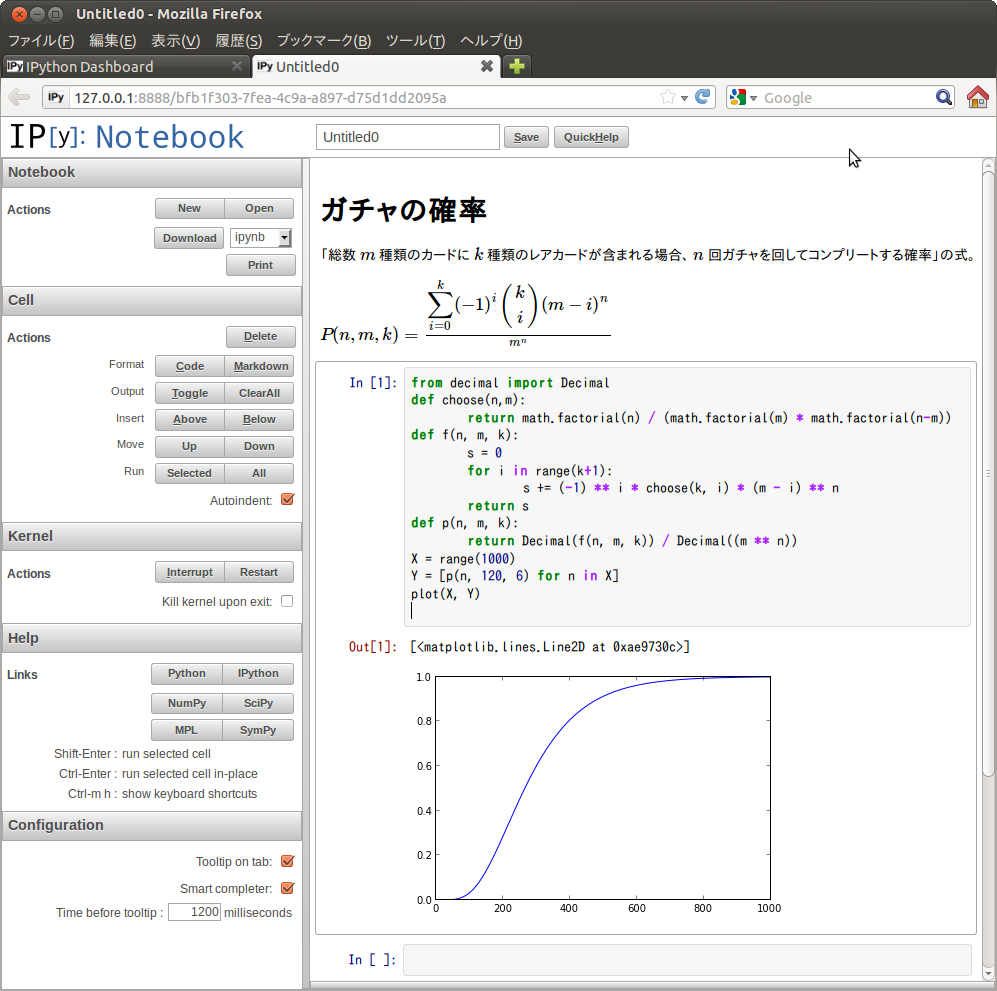
\includegraphics[width=0.80\hsize]{image2012-gum/ipython-gacha.png}
  \end{center}
  \caption{ipython notebookの使用例}
  \label{fig:ipython-gacha}
\end{figure}

testingには次のコマンドでインストール可能です。

\begin{commandline}
$ sudo aptitude install ipython-notebook python-matplotlib python-tornado
\end{commandline}

squeezeはqtconsoleと同様にbackportsを使用します。
ここではsqueezeのiceweaselが古いためこちらもapt lineに追加しています。

\begin{commandline}
deb http://backports.debian.org/debian-backports squeeze-backports main
deb http://mozilla.debian.net/ squeeze-backports iceweasel-release
\end{commandline}

\texttt{aptitude update \&\& aptitude upgrade}を実行した後、
インストールは次のコマンドで行いました。

\begin{commandline}
$ sudo aptitude install python-setuptools python2.6-dev ncurses-dev libzmq-dev python-pygments python-matplotlib
\end{commandline}

パッケージをインストールした後、
pythonの\texttt{easy\_install}コマンドを使用してipythonをインストールします。

\begin{commandline}
$ sudo easy_install readline pyzmq ipython tornado
\end{commandline}

またこのままではMathJaxがCDNを指しているので、
pythonを管理者権限で実行しローカルにインストールします。

\begin{commandline}
from IPython.external.mathjax import install_mathjax
install_mathjax()
\end{commandline}

squeezeのウェブブラウザはどれも古く、
Web Socketの問題からnotebookでは使えません。
そこで最新版のiceweaselを導入します。
ipython notebookは起動時にデフォルトブラウザを起動するため、
導入後はiceweaselをデフォルトブラウザに指定してください。

\begin{commandline}
$ sudo aptitude install -t squeeze-backports iceweasel
\end{commandline}

ipython notebookは次のコマンドで起動します。

\begin{commandline}
$ ipython notebook --pylab inline
\end{commandline}

他のマシンから接続を行う場合、
ブラウザを起動させないためオプション``\texttt{--no-browser}''を、
アクセス許可を与えるためnotebookを起動させるマシンのipアドレスをオプション``\texttt{--ip}''で指定します。

\begin{commandline}
$ ipython notebook --pylab inline --no-browser --ip 192.168.1.40
\end{commandline}

初回起動時には次のような画面が表示されます。

\begin{figure}[ht]
  \begin{center}
    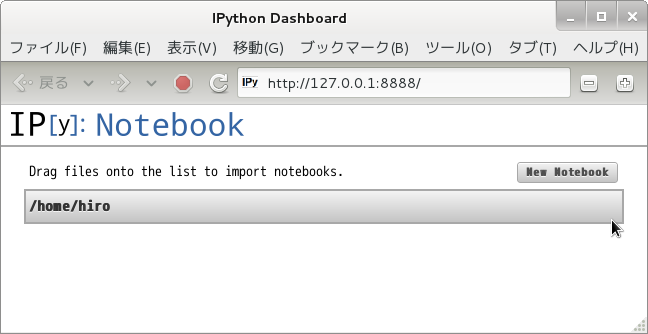
\includegraphics[width=0.67\hsize]{image2012-gum/ipython-notebook.png}
  \end{center}
  \caption{ipython notebookを起動した直後}
  \label{fig:ipython-notebook}
\end{figure}

「New Notebook」ボタンをクリックすることで新規ノートブックが作成され、
空のノートブックがブラウザに表示されます。
MarkdownとPythonのCellは\texttt{Ctrl-m m}および\texttt{Ctrl-m c}で切り替えることができ、
その他コマンドの詳細は\texttt{Ctrl-m h}で表示されます。

作成されたノートブックは表示されているディレクトリ(ここでは/home/hiro/)に``$<$ ノートブックのタイトル$>$.ipynb''というファイル名で保存されます。
このファイルの中身はJSON形式となっています。

\subsection{最後に}

今回はipython qtconsoleおよびnotebookをDebianで使用する方法を紹介しました。
Ubuntu 12.04ではどちらもパッケージとして提供されているため、
wheezyではインストール作業が簡単になると思われます。
これを機会にipythonを活用していただければ幸いです。


%------------------------------------------------------------------------------
\dancersection{DebianとLibreOffice}{あわしろ いくや}
\label{sec:libreoffice}
%------------------------------------------------------------------------------

\subsection{自己紹介}
\subsection{OOoのあらすじ}

\begin{itemize}
\item 1999/8/??…Sun MicrosystemsがStarOfficeの開発企業を買収
\item 2000/10/13…後にOOoとなるソースコード公開
\item 2002/5/1…OOo 1.0リリース
\item 2009/4/20…OracleによるSunの買収を発表
\item 2010/1/27…Oracleによる買収完了
\item 2010/6/4…OOo 3.2.1リリース
\item 2011/1/25…最終バージョンの3.3.0リリース
\end{itemize}

\subsection{LibreOffice その1}

\begin{itemize}
\item 2010/9/28…The Document FoundationとLibreOfficeのリリースを発表
\item OOoのコミュニティメンバーで結成
\item OOoの商標の移譲をOracleに求めてみたり
\item 2011/1/25…LibreOffice 3.3.0リリース
\item 2011/6/3…LibreOffice 3.4.0リリース
\item 2012/2/14…LibreOffice 3.5.0リリース
\item 2012/2/20…TDFが財団に
\end{itemize}

\subsection{LibreOffice その2}
\subsubsection{かなり普通の開発体制になった}

\begin{itemize}
\item ソースコードはgitで管理
\item 契約書にサインしなくてもpushされる
\item ライセンスはLGPLとMPL
\item 毎月リリース、半年に1度メジャーバージョンアップ
\item 今は8月リリースに向けて3.6を開発中
\end{itemize}

\subsection{Apache OpenOffice}

\begin{itemize}
\item 2011/4/15…OracleがOOoの開発中止を発表
\item 2011/4/20…担当社員を全員解雇
\item 2011/6/1…Apacheへの移管を発表
\item 2011/6/13…ApacheのIncubatorプロジェクトに承認
\item 2011/11/17…名称を”Apache Openoffce”に決定
\item 2011/11/31…ライセンスをAL 2に変更する作業完了
\item 2012/5/8…AOO 3.4.0リリース
\item 2012/5/17…AOO 3.4.0 100万ダウンロード
\item 2012/5/21…Lotus Symphonyのコード公開
\item 2012/5/27…AOO 3.4.0 200万ダウンロード
\end{itemize}

\subsection{Apache OpenOffice その2}
\subsubsection{Lotus Symphony}
\begin{itemize}
\item IBMが2008/5/30にリリース
\item OOoとEclipseをベース
\item Sunから特別なライセンス
\item ワープロ・表計算・プレゼン・Webブラウザ
\item Windows/Linuxで動作
\item 無償配布
\item 2012/1/23…最終バージョンの3.0.1リリース
\end{itemize}

\subsection{OOo meets Debian}
\subsubsection{最初のアップロードは2001/10/23}

\begin{itemize}
\item 2002/4/24…0.641d.cvs20020424-1をアップロード
\item 2002/5/1…OOo 1.0リリース
\item 2002/5/2…OOo 1.0 sid入り
\item 2002/7/11…OOo 1.0.1 sid入り
\end{itemize}

\subsubsection{現在のメンテナンス体制}

\begin{itemize}
\item Rene EngelhardさんとBj\"{o}rn Michaelsenさん(Canonical)の二人体制
\item とはいえ、パッケージに関してはReneさんの作業量が多い
\item Bj\"{o}rnさんはupstreamの作業が多い
\item Bj\"{o}rnさんはビルドのスペシャリスト、Reneさんはパッケージングのスペシャリスト
\end{itemize}

\subsection{LibOfficeのパッケージの背景}

\begin{itemize}
\item OOo 3.3.0に関する作業が行われた形跡が全くない
\item 以前はベータ版でも作業が行われていた
\item Reneさんはかなり早い段階からTDFに誘われていたことがわかる
\item 確かにFounderの一人になっている\\
\url{http://www.documentfoundation.org/foundation/history/}
\item その時点でLibOがDebianに入ることは確定的だった
\item LibOがsidで使えるようになったのが2012/2/6
\item 現在でもOpenOffice.orgのパッケージはあるものの、LibreOfficeへの移行用ダミーパッケージ
\end{itemize}

\subsection{LibreOfficeパッケージ}

\subsubsection{libreoffice-3.5.3を例に}

\begin{itemize}
\item ソースを取得後df -hすると3.2GB
\item rulesをwc -lすると3146
\item controlをwc -lすると3380
\item changelogをwc -lすると9763
\item builddでのビルド時間は6時間40分(i386)
\item 必要なディスクスペースは17.04GB
\item パッチはquiltで管理
\end{itemize}

\subsubsection{Debian パッケージの注意点}

\begin{itemize}
\item 得てしてオフィシャルのバイナリを前提とした説明をされる
\item 拡張機能は一切インストールされないので、あとからインストールする。たいていはパッケージ化されている
\item libreoffice-gnome/libreoffice-gtk3/libreoffice-kdeのインストールを忘れない
\end{itemize}

\subsection{LibOffice 関連パッケージ}

\begin{enumerate}
\item ooohg \\
Set of 1600 free of charge maps for libreoffice/openoffice.org
\item openclipart-libreoffice \\
clip art for OpenOffice.org/LibreOffice gallery
\item writer2latex \\
OpenOffice.org Writer/Calc to LaTeX/XHTML converter
\end{enumerate}

\subsection{翻訳のこと}
\subsubsection{皆さんにお願い}
\begin{itemize}
\item \url{discuss@ja.libreoffice.org}を購読してね
\item 翻訳の指摘(誤訳やわかりにくいものなど)
\item 専門的な知識の教示
\item 英語、日本語、ワープロ、表計算(特に関数)、ドロー、Windows、Mac、Linux、数式、データベース、PDF、印刷 etc...
\item 間接的にDebianへの貢献にもなりますよ!
\end{itemize}

\subsection{AOO と Debian}
\subsubsection{6月上旬現在、パッケージなし}
\begin{itemize}
\item 怪しいリポジトリはある\\
\url{http://apacheoo-deb.sourceforge.net/}
\item オフィシャルビルドのDebパッケージをaptで取れるようにしているだけ
\item ちなみにlaunchpadにプロジェクトはあるけどパッケージはない\\
\url{https://launchpad.net/~apacheopenoffice}
\end{itemize}

\subsubsection{オフィシャルビルドのDebパッケージ}
\begin{itemize}
\item EPMで生成
\begin{itemize}
\item ESP Package Manager
\item これはLibreOfficeも一緒
\item 原作者はCUPSの作者
\item RPMとかDebパッケージを生成するもの
\item すなわち、debianフォルダがあるわけじゃない
\item どうやってもオフィシャルにならない
\end{itemize}
\end{itemize}
\subsubsection{3月にdebian-usersとdebian-openofficeでAOOに関する投稿あり}
\begin{itemize}
\item \url{http://lists.debian.org/debian-user/2012/03/msg00824.html}
\item \url{http://lists.debian.org/debian-openoffice/2012/03/msg00103.html}
\end{itemize}
いずれもReneさんが激しく拒否

\subsection{さらなる情報}
\subsubsection{主に歴史を知りたい人向け}
\begin{enumerate}
\item 2011年のOpenOffice.org/LibreOffice
\\
\url{http://gihyo.jp/lifestyle/column/newyear/2011/openoffice-prospect}
\item LibreOffice/Apache OpenOffice 〜2011年の総括と新たな選択〜
\\
\url{http://gihyo.jp/lifestyle/column/newyear/2012/libreoffice-prospect}
\end{enumerate}

%------------------------------------------------------------------------------
\dancersection{debug.debian.net}{岩松 信洋}
\label{sec:debug.debian.net}
%------------------------------------------------------------------------------

\subsection{はじめに}
現在、Debian Project で配布されているパッケージでは、
デバッグ情報が削除された状態で配布されています。
この理由として、デバッグ情報はほとんどのユーザには必要ないものであるという点と、
デバッグ情報を保持している実行ファイルはサイズが非常に大きいため、ディスクを圧迫
するという点があります。
しかし、デバッグ情報があるとデバッグを行うときにとても有用な情報となりいろいろと便利です。
今回、Debian で全てのDebianパッケージにおいてデバッグ情報を提供する方法を考えて実装してみま
した。その課程と今後について説明します、

\subsection{Debug情報とDebianパッケージ}
Debian はバイナリベースディストリビューションの一つです。
基本的に配布されているパッケージではデバッグ情報が削除された状態で配布されています。
このデバッグ情報は、内部シンボルや型の情報、ソースコードの行番号などを指します。

実行ファイルのデバッグ情報がある場合、以下のようなよい点があります。
\begin{itemize}
\item デバッガ(GDB)を使ったデバッグでより詳細なデバッグ情報を得ること
ができる
\item デバッグ情報を含めたバイナリを再度ビルドする必要がない
\item バイナリベースディストリビューションの場合、実際のバイナリとデバッグ情報が常に
対になるので、バグの再現性が高くなる
\end{itemize}
%これらは組み込み用途にもよく利用されているDebianでは特に有効に働きます。
%また、デバッグ情報を含めるためのパッケージ作成方法(DEB_BUILD_OPTIONS=nostrip をを環境
%変数にエクスポートする)を調べる必要もありません。

逆に悪い点として以下のようなものがあります。

\begin{itemize}
\item 実行ファイルにデバッグ情報が含まれるので実行ファイルのサイズが大きくなる
\item デバッグしない人にとっては不要なものが含まれることになる
\end{itemize}

これらをまとめると、すべての実行ファイルのデバッグ情報が提供されており
ユーザにとって必要のない情報がインストールされない仕組みがあれば
デバッグ情報はとても有益なものになるはずです。
Debian ではいくつかのソースパッケージからデバッグ情報を含んだパッケージが提供されています。
このパッケージには\texttt{-dbg} というサフィックスが付いてます。
特にデバッグ情報用のパッケージに関するポリシーは決まっておらず、提供に関してはパッケージメンテナ
次第という状態になっています。今まで提供されなかった理由としてはディスク容量の問題や回線の
問題等があったようですが、個人的に今は特に問題はないと思っています。

ちなみに、Fedoraでは \texttt{-debuginfo} というサフィックスを持ったパッケージが提供されており、
Gentooではデフォルトでこれらの情報を生成し管理しています。このようにデバッグ情報の提供という点に
関して他のディストリビューションに遅れを取っています。

\subsection{Debianでのデバッグ情報パッケージについて}
まず、実装した内容について説明する前に今のデバッグ情報パッケージの提供方法について説明します。
Debianではデバッグ情報パッケージは \texttt{-dbg} というサフィックスがついたパッケージ名を持ちます。
例えば foo というアーキテクチャ依存のパッケージがあった場合、\texttt{foo} のデバッグ情報を持ったパッケージ名は
\texttt{foo-dbg} になります。
そして、Debian の \texttt{-dbg} パッケージで提供されているバイナリは動作するバイナリデータではなく、
デバッグ情報のみを持ったデータになっています。 このファイルは \texttt{objdump --only-keep-debug}
を実行することによって生成することができます。もちろん対象の実行ファイルはコンパイル時にデバッグ情報
が付加されている必要があります。
その後、デバッグ情報ファイルへのリンクを \texttt{strip} 済の実行可能形式に付加するために
\texttt{objcopy --add-gnu-debuglink} を実行します。
これによって、実行ファイルとデバッグ情報ファイルが対になります。
GDB を使ってデバッグする際には実行ファイルとデバッグ情報ファイルはリンク
しているので、デバッグ情報ファイルがインストールされているときは自動的に呼ばれ、デバッグ
シンボルなどを読み込んでくれます。

\subsection{実装について}

先に説明したようにに、すべての実行ファイルのデバッグ情報が提供されており
ユーザにとって必要のない情報がインストールされない仕組みがあればよいので、
これらに対応できる方法を考えました。以下で説明します。

\subsubsection{すべての実行ファイルのデバッグ情報を提供する}
すべての実行ファイルのデバッグ情報を提供するには、全てのパッケージで
\texttt{strip} された実行ファイルとデバッグ情報ファイルを持ったパッケージを構築すれば
よいわけです。


Debian の場合、パッケージはデバッグ情報が有効な状態(\texttt{gcc} だと\texttt{-g} オプション等)
でビルドされます。そしてパッケージにされる時に \texttt{strip} (binutilsに含まれる)
が \texttt{dh\_strip} から呼ばれ、実行ファイルやライブラリならデバッグ情報が削除され、
パッケージ用のディレクトリにコピーされ、\texttt{dh\_builddeb} コマンドでパッケージ化されます。

そして、配布される -dbg パッケージは \texttt{dh\_strip}を実行するときにデバッグ情報を提供する
パッケージとして、\texttt{dh\_strip} のオプションとして指定されるか、debian/control ファイルに列挙されている
パッケージ名のサフィックに \texttt{-dbg} が付いている場合、対象ファイルとして処理されます。

ここ問題なのが、
\begin{enumerate}
\item 自動生成したい デバッグ情報パッケージ情報をどのように生成するか
\item \texttt{dh\_strip} でデバッグ情報パッケージ指定されている場合、自動生成したい -dbg パッケージ用のファイルを
どのように生成するか
\item 自動生成したいデバッグ情報パッケージそのものをどのように生成するか
\end{enumerate}
という点です。

問題点1についての対処方法ですが、\texttt{dh\_strip} の処理の先頭で debian/control ファイルに
デバッグ情報パッケージファイルに関する情報を追記する処理を追加しました。
デバッグ情報パッケージはそのパッケージがアーキテクチャ依存(Architechture: all ではない)
事とパッケージ名さえわかれば、パッケージ情報は自動生成できます。
例えば、\texttt{hoge} というパッケージがあってデバッグ情報パッケージが提供されていない場合、
以下のような内容を追記します。

\begin{commandline}
Package: hoge-dbg
Architecture: any
Section: debug
Priority: extra
Depends: hoge (= \${binary:Version}), \${misc:Depends}
Description: debugging symbols for hoge
 This package contains the debugging symbols for hoge
\end{commandline}

次に問題点2の対処方法ですが、アーキテクチャ依存のDebianパッケージは \texttt{dh\_strip} が呼ばれるため、ここで
処理をフックしてしまえば、デバッグ情報を提供するパッケージと用のデータと \texttt{strip} された
バイナリデータを分けることができます。今回は \texttt{dh\_strip} の中身を改造し、全てのアーキテクチャ依存の
パッケージ用のデータを作成することにしました。\texttt{dh\_strip}でパッケージが指定されていても
それを無視するように処理を変更するだけです。

問題点3の対処方法ですが、デバッグ情報パッケージは \texttt{dh\_strip} 内で \texttt{dh\_builddeb} を呼び出すことで
対応しました。パッケージ名とパッケージ作成に必要なデータは揃っているので、
\texttt{dh\_builddeb -pデバッグ情報パッケージ名} を実行することで、パッケージが作成されます。

これらが行える前提条件として、debhelper に依存しているパッケージが対象になります。
現在ほとんどのパッケージが debhelper か CDBS に依存しており、CDBS は debhelper と
同時に使う事が多いため(実際、CDBSに依存しているパッケージは全てdebhelper に依存しています。dbsも同様です。)
問題ではありません。
\footnote{\url{http://people.debian.org/~cjwatson/dhstats.png}}

\subsection{パッケージサイズへの対応}

次にパッケージサイズの問題です。
デバッグ情報は非常に大きく、\texttt{strip} されたバイナリの数倍以上のサイズになることは
めずらしくありません。例えば libjpeg8 で提供される libjpeg.so.8.4.0 のファイル
サイズは表\ref{tab:debuginfo-jpegsize}となりました。

\begin{table}[ht]
 \caption{libjpeg.so.8.4.0 各状態のファイルサイズ}
 \label{tab:debuginfo-jpegsize}
\begin{center}
  \begin{tabular}{|c|c|}
 \hline
 状態 & サイズ \\
 \hline
 strip 前 & 約1.3MB \\
 strip 後 & 236KB \\
 デバッグ情報ファイル & 1.1MB \\
 \hline
 \end{tabular}
\end{center}
\end{table}

このようにサイズが大きく異なるので、パッケージを分けてもユーザが利用しているパッケージリポジトリ
と同じ場所・方法で提供してしまうと、ミラーに時間がかかるようになりますしユーザに不要なデータが格納されたリ
ポジトリ情報を持たせるようになります。

今回、この問題を回避するためにリポジトリを分けることを考えました。
例えば、unstable で \texttt{strip} されているパッケージ(通常のパッケージ)は unstable とだけ指定し、
デバッグ情報を提供するパッケージは unstable/debug するという方法です。
例を図\ref{fig:debuginfo-apt-line}に示します。

\begin{figure}[ht]
\begin{center}
\begin{commandline}
deb http://cdn.debian.or.jp/debian/ unstable main non-free
deb http://cdn.debian.or.jp/debian/ unstable/debug main
\end{commandline}
\end{center}
 \caption{デバッグ情報パッケージを利用する場合の apt-line 設定例}
 \label{fig:debuginfo-apt-line}
\end{figure}


デバッグ情報が必要なユーザは unstable/debug を apt-line に追加することによってデバッグ情報
用のパッケージが利用できるようになります。
またパッケージが格納されるディレクトリのパスを変更することによって、デバッグ情報のみを
提供するミラーを構築することができ、debug 情報をミラーしないミラーサーバの負荷も今までと変わ
らないという事になります。

\subsubsection{実装後について}

これらを実装したシステムを reprepro + sbuild + rebuildd で構築しました。
現在stable/amd64のみをターゲットテストとして動作させています。
まだ全てビルドできていません。さくらのVPSで1週間ほどビルドしていますが、
まだgnome-power-managerをビルドしているところで、進捗率は40\%といったところでしょうか。

\subsection{考えられる問題}

\subsubsection{セキュリティの問題}
現在、ソースパッケージから作成されたバイナリバッケージの一覧は .changesファイルに
ファイルのハッシュと共に記述され、どのソースパッケージ(orig.tar.gz, dsc.diff.gz)
から作成されたのか分かるようになっています。
現時点での実装はバイナリパッケージ作成の課程で自動生成されるためのこれらの情報
とリンクしません。Buildd上でデバッグ情報ファイルパッケージが生成されるので個人的に
問題ないと思っていますが、これらを紐付けるシステムがあるほうがより安全と言えるでしょう。

\subsubsection{バイナリの不一致}
既存のシステムだと、\texttt{strip} されたバイナリと デバッグ情報が一致しないので
オフィシャルのバイナリと混ぜて使えないことが考えられます。私が提供している
されているデバッグ情報パッケージを使う場合、
私が提供してる通常のパッケージも利用しないと意味がないでしょう。
今はこれをバージョンによる依存関係で回避しています。
最終的には buildd に入れてもらうことでデバッグ情報パッケージを自動生成することを
考えています。

\subsection{そもそも debug.debian.netがあるんじゃね?という話}
さて、私のような凡人が考えるようなことは先人達はすでに考えているわけでして、
(既に行なっていることを知ったのは大統一勉強会スケジュールが出てからなのですが。)
既に \url{http://debug.debian.net}というサービスがあり実装され、そして終了していました。
実装と考えもほとんど同じです。大きく違うところはデバッグ情報パッケージの
サフィックスが\texttt{-dbg}ではなく、\texttt{-dbgsym}である点と、
デバッグ情報を作成する部分が \texttt{dh\_builddeb} ではなく、\texttt{dpkg-deb} を使っている
点、そして\texttt{dh\_strip}を直接変更するのではなく、シンボリックリンクで
機能をオーバーライドさせている点です。こちらの方がdebhelperに手を加えなくて済むので
こちらに乗り換えて、いくつかの修正を行いました。
元々このサービスは myon \footnote{Christoph Berg氏。DAM の一人。} がやっていたのですが、
彼に連絡を取り、再稼働させることにしました。この発表が行われている頃には稼働していると思います。

\subsection{今後の課題}

このままスタンドアロンでデバッグ情報パッケージを提供しても無駄なバイナリを生成するだけなので、
buildd にこのシステムを入れてもらい、dak で ディストリビューション/debug として
処理してもらうことが今後の大きな課題になっています。このことについて来月開催される Debconf 12
でBOF またはFTPチーム、wanna-builddチームと話ができればと思っています。

\subsection{最後に}
アーキテクチャに依存している Debian パッケージでデバッグ情報を
パッケージとして提供する方法について説明しました。文中ではユーザには
あまり必要のない機構のように取り扱いましたが、バグレポートをする際、
デバッグ情報があるとより内容の濃いバグレポートを提出できるようになり、
開発者を手助けできるようになります。この機構が正式採用された時に、
自分が使っているパッケージのデバッグ情報パッケージだけでもインストール
してくれれば幸いです。

%------------------------------------------------------------------------------
\dancersection{Rabbit: 時間内に終われるプレゼンツール}{須藤功平}
\label{sec:Rabbit}
%------------------------------------------------------------------------------

% add upper space for logo
\vspace{2em}

Debian GNU/Linux上で動作するプレゼンテーションツールRabbitを紹介します。
まず、Rabbitの代表的な機能である時間内に終われるための機能を紹介し、そ
の後、Debian GNU/Linux上でRabbitをインストールする方法とスライドを作る
方法を簡単に紹介します。

\subsection{Rabbitとは}

RabbitはRubyとGTK+で実装されたプレゼンテーションツールです。Debian
GNU/Linuxを含む多くのプラットフォーム上で動作します。

Debian GNU/Linux上で動作するプレゼンテーションツールはたくさんあります。

\begin{itemize}
\item GUIでスライドを作成するデスクトップアプリケーション
  (LibreOfficeのImpressなど)
\item テキストで作成したスライドを表示するデスクトップアプリケーション
  (MagicPointやRabbitなど)
\item \LaTeX{}のBeamerクラス + PDFビューアー(Evinceやpdfcubeなど)
\item JavaScript + Webブラウザ(Impress.jsやshowoffなど)
\item Webサービス(Google DocsやPreziなど)
\end{itemize}

それぞれのツールは特徴が大きく異なっており、それぞれよいところがありま
す。Rabbitにもまた特徴があり、他のツールにはない便利な機能があります。
それが「プレゼンテーションを時間内に終われるための機能」です。この機能
は一般的にタイマー機能と呼ばれているもので、プレゼンテーション中に残り
時間を表示して、発表者に進み具合を伝える機能です。多くのツールでこの機
能を提供していますが、Rabbitのタイマー機能はどう違うのでしょうか。一言
でいうとUI(ユーザーインターフェイス。見た目)が違います。他は同じで
す。

\subsubsection{RabbitのUI}

タイマー機能はMagicPointも提供していますし、Impressも提供しています。
図\ref{fig:normal-timer-ui}のように、MagicPointはスライド下部にとても目
立たないように緑のバーを表示します。Impressはスライド表示用のモニターと
は別のモニターに経過時間を表示します。このように発表者にだけわかるよう
に表示するUIが一般的なタイマー機能のUIです。

\begin{figure}[ht]
  \begin{center}
    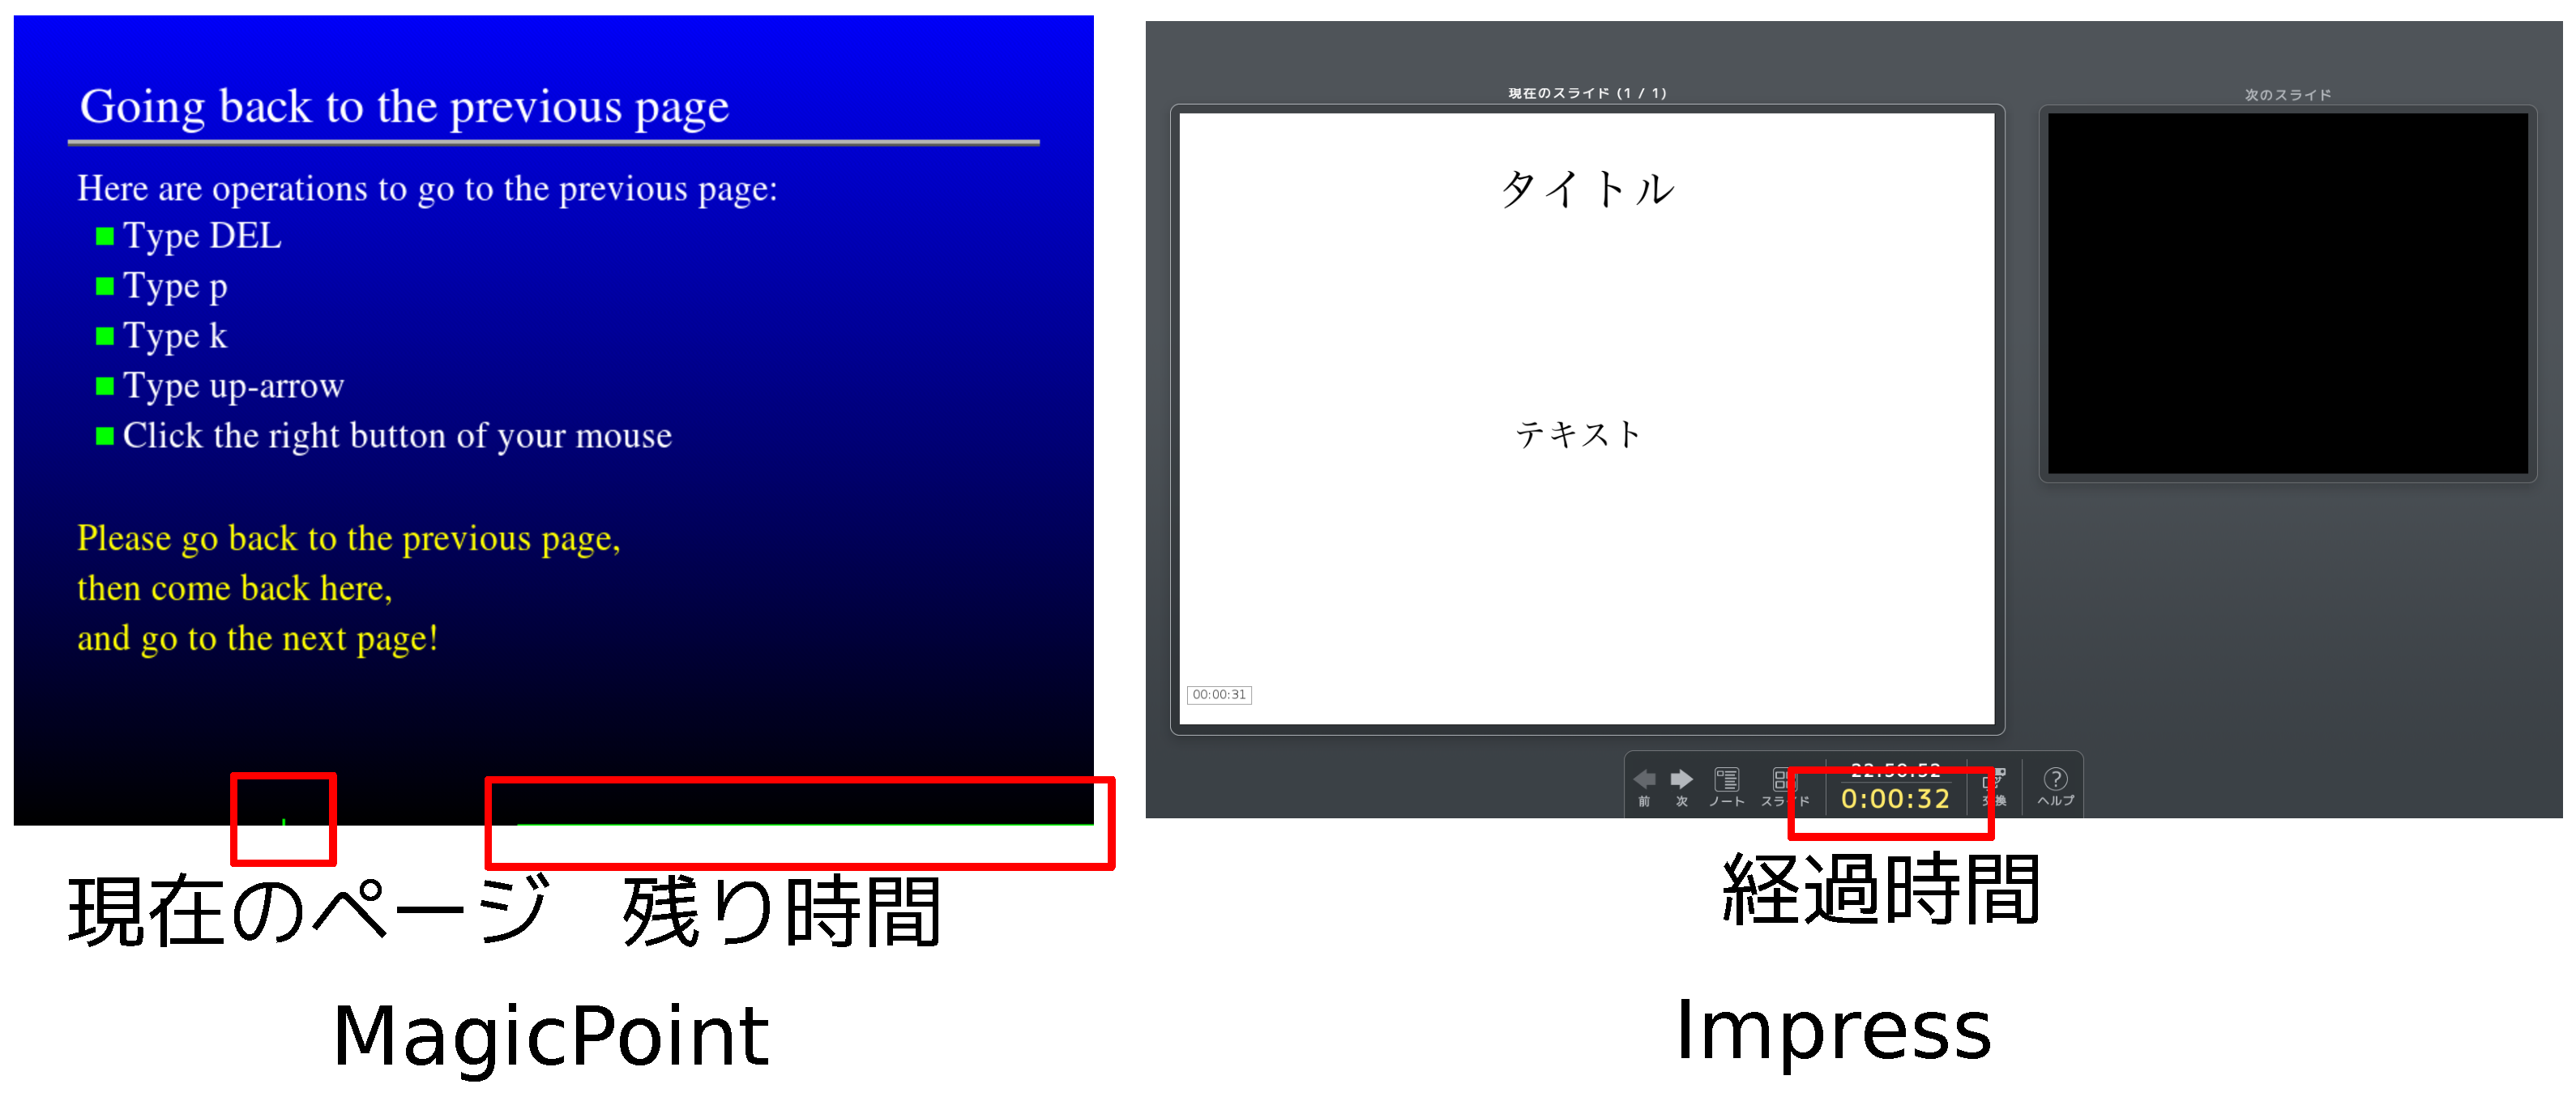
\includegraphics[width=1\hsize]{image2012-gum/normal-timer-ui.eps}
  \end{center}
  \caption{従来のタイマー機能のUI}
  \label{fig:normal-timer-ui}
\end{figure}

一方、RabbitのUIは発表者だけではなく観客にもわかりやすく表示します。
図\ref{fig:rabbit-timer-ui}のように、スライド下部にうさぎとかめを表示し
ます。それも誰が見ても気づくくらいの大きさで表示します。このようにタイ
マー機能を観客からもわかりやすく表示するUIは既存のプレゼンテーションツー
ルとは一線を画します。

\begin{figure}[ht]
  \begin{center}
    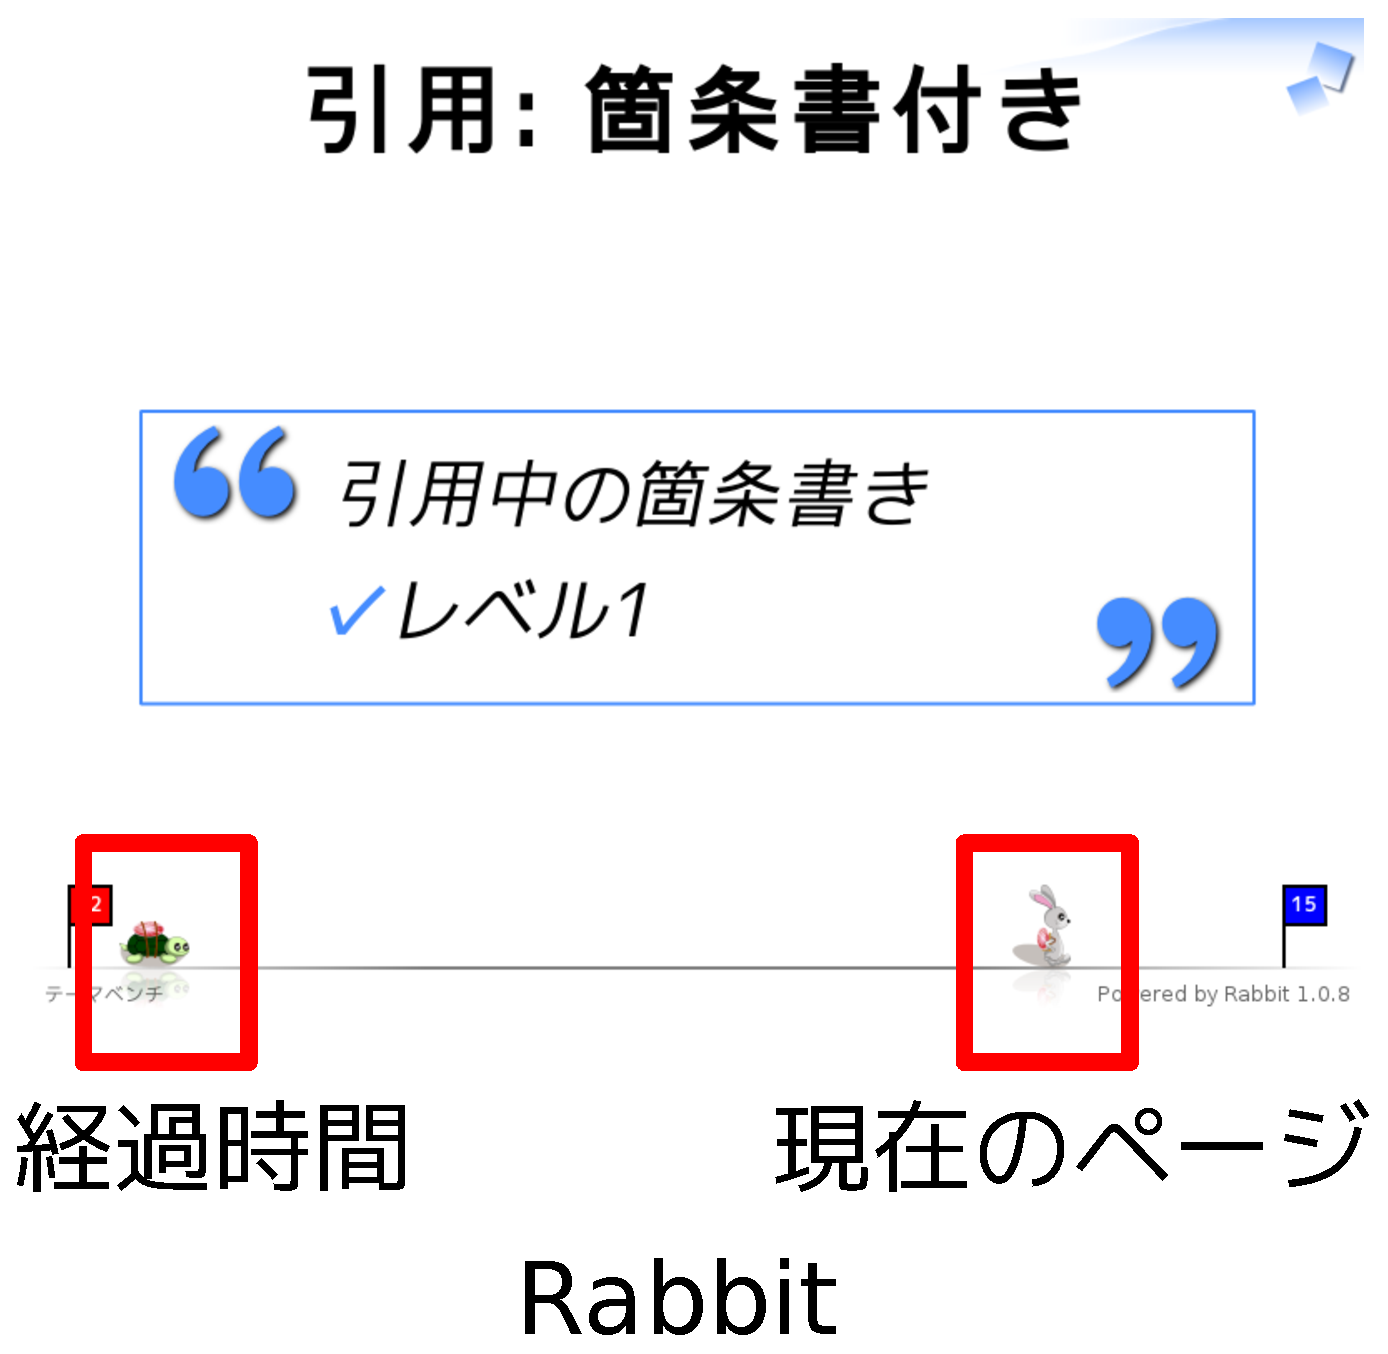
\includegraphics[width=0.5\hsize]{image2012-gum/rabbit-timer-ui.eps}
  \end{center}
  \caption{Rabbitのタイマー機能のUI}
  \label{fig:rabbit-timer-ui}
\end{figure}

それでは、このUIがどうして時間内に終わるための効果を提供するかを考えて
みましょう。

\subsubsection{みんなにわかるUI}

このRabbitのUIの特徴は発表者だけではなく、観客にも発表の進み具合がわか
りやすいという点です。発表時間を過ぎれば経過時間を表しているかめが画面
の右側に走りすぎていきます。もちろん、かめなので徐々に画面の右側に進ん
でいきます。そのため、観客が気づかないうちに発表時間を過ぎていたという
ことは起きません。発表時間を過ぎても終わらないと、たとえどれだけ魅力的
な話であっても気まずい空気になってきます\footnote{要出典。}。

発表者は観客の反応がよいとよりすばらしい発表ができますが、逆に反応が悪
いと、準備してきた成果を発揮しづらいものです。発表時間が過ぎても終わら
ない場合、観客の反応が悪くなります。この状態でさらに続けることはとても
つらいため自然と終わらせようという力が働きます。

このように、タイマー機能を発表者だけではなく観客からもわかりやすいUIに
することにより、観客から残り時間に関するフィードバックを受け取ることが
できます。発表者が残り時間を意識するだけではなく、観客からのフィードバッ
クもあわせることで自然と時間内に終われる発表になります。ただし、観客に
わかりやすいタイマー機能のUIなので、発表内容よりもうさぎとかめの競争に
集中してしまい、肝心の発表内容に集中してもらえないという危険性がありま
す。時間内に終わることだけではなく、魅力的な発表内容を用意することにも
十分注意してください。

\subsection{インストール方法}

ここまでの紹介でRabbitを使いたくなっているはずです。ここからはRabbitの
使い方を紹介します。

まず、RabbitをDebian GNU/Linuxへインストールする方法を紹介します。イン
ストール方法は2種類あります。

\begin{itemize}
\item aptを使う
\item RubyGemsを使う
\end{itemize}

最新バージョンを使いたい場合やフル機能を使いたい場合はRubyGemsを使う方
法がオススメです。簡単にインストールしたい場合はaptを使う方法がオススメ
です。

\subsubsection{aptでインストール}

1つ目の方法は、aptを使う方法です。Rabbitのdebパッケージは公式aptリポジ
トリに含まれている\footnote{大統一Debian勉強会の実行委員でもある佐々木
  洋平さんがパッケージメンテナー。}ので以下のようにすれば簡単にインストー
ルできます。

\begin{commandline}
$ sudo apt-get -V -y install rabbit
\end{commandline}
%$
以下のコマンドを実行してスライドが表示されたら正常にインストールできています。

\begin{commandline}
$ rabbit https://raw.github.com/shockers/rabbit/master/sample/theme-bench.rab
\end{commandline}
%$
\subsubsection{RubyGemsでインストール}

2つ目の方法はRubyGemsを使う方法です。RabbitはGTK+などたくさんのライブラ
リを利用しています。そのため、まず、関連ライブラリをaptでインストールし
ます。

\begin{commandline}
$ sudo apt-get -V -y install \
    ruby1.9.1 ruby1.9.1-dev libgtk2.0-dev librsvg2-dev libpoppler-glib-dev \
    libxml2-dev libxslt1-dev
\end{commandline}
%$

関連ライブラリをインストールしたらRubyGemsでRabbitをインストールします。

\begin{commandline}
$ sudo gem1.9.1 install rabbit twitter-stream twitter_oauth
\end{commandline}
%$

以下のコマンドを実行してスライドが表示されたら正常にインストールできています。

\begin{commandline}
$ PATH="/var/lib/gems/1.9.1/bin:$PATH"
$ rabbit https://raw.github.com/shockers/rabbit/master/sample/theme-bench.rab
\end{commandline}
%$
\subsection{スライドの作り方}

Rabbitを使う準備ができたので自分でスライドを作る方法を紹介します。

RabbitはMagicPointのようにテキストでスライドを作成します。テキストの
フォーマットにはRD\footnote{Ruby Documentの略。}やWiki形式、Markdownな
どいくつもの有名なフォーマットをサポートしています。ここでは、RDでのス
ライドの書き方を紹介します。

\subsubsection{RDでのスライドの作り方}

RDでスライドを作る場合、以下のように「{\tt{=}}」でスライドを区切ります。
「{\tt{=}}」の行に書いているテキストがそのスライドのタイトルになります。
「{\tt{\#}}」から始まる行はコメントです。シンプルですね。

\begin{commandline}
# slide.rab

= タイトルスライド

# 持ち時間
: allotted-time
   5m

= 最初のスライド

  * 1枚目のスライドの内容

= 2枚目のスライド

  * 2枚目のスライドの内容
\end{commandline}

最初のスライドは特別でタイトルスライドになります。ここにはスライド全体
のメタデータを指定することができます。「{\tt{allotted-time}}」というのは
このプレゼンテーションの持ち時間で、「{\tt{5m}}」は5分\footnote{5
  Minutes}という意味です。持ち時間を指定するとうさぎとかめタイマーが表
示されるので、持ち時間が決まっているプレゼンテーションのときは指定しま
しょう。

作成したスライドは以下のように実行します。2ページ目を表示するとうさぎと
かめタイマーが動きだします。

\begin{commandline}
$ rabbit slide.rab
\end{commandline}

\subsubsection{PDFで作成したスライドの表示方法}

Rabbitはスライドを表示する機能だけを提供しているため、スライド作成を支
援する機能はありません。Debian GNU/Linuxを使っている人はエディターでテ
キストを編集することに慣れているでしょうが、たまにはImpressなどを使っ
てGUIでグラフィカルにスライドを作成したくなるかもしれません。そのときは
そのようなツールでスライドを作成してください。Rabbitはテキストだけでは
なくPDFファイルも読むこむことができます。Impressなどでスライドを作成
しPDFで出力すれば、Rabbitで表示することができます。

PDFを表示するときはコマンドラインから持ち時間を指定します。
「{\tt{--allotted-time 5m}}」と指定すると持ち時間が5分という意味になりま
す。2ページ目を表示するとうさぎとかめタイマーが動きだします。

\begin{commandline}
$ rabbit --allotted-time 5m slide.pdf
\end{commandline}

\subsection{さいごに}

Debian GNU/Linux上で動作する時間内に終われるプレゼンテーションツー
ルRabbitを紹介しました。Debian GNU/Linuxでプレゼンテーションをする人た
ちの参考になることを期待しています。

もっとRabbitを知りたくなった人は公式サイ
ト\url{http://rabbit-shockers.org/}をのぞいてみてください。

%------------------------------------------------------------------------------
\dancersection{U-Bootについてあれこれ}{野島 貴英}
\label{sec:u-boot-arekore}
%------------------------------------------------------------------------------

\vspace{2em}
% Add upper space for logo

Debianは組み込み用途の開発にも非常に便利の良い開発環境を作る事ができます。
ここでは、組み込み用途の開発では最も基本的なソフトウェアであるブートローダ
をDebianの環境を用いてU-Bootを用いて開発してみます。最後に、電子書籍端末に
ブートローダを実際に搭載して起動を試みます。

\subsection{U-Bootとは}

U-Bootとは、DENX Software Engineering社(本家)で主にメンテされている
ブートローダです。Das U-Bootともいう\footnote{ドイツ語で潜水艦の意。この場合直訳すると「ザ・潜水艦」と言う感じです。}そうです。

元はPowerPC用途のブートローダだった模様ですが、様々な人が拡張を加え、現在では216種類の組み込み機材に対応しており、さらに対応数は増えつづけてている模様です\cite{u-boothistory}。

\subsection{U-Bootの特徴}

以下に示す沢山の特徴があります。

\begin{itemize}
\item ソフトウェアライセンスはGPL v2です
\item 沢山のCPU、組み込み機材に対応しています。例:PowerPC,ARM,AVR32,Blackfin,m68k,x86,...
\item U-Bootのソース本体は単機能の部品の塊であり、ディレクトリも十分に整理され、マクロも整理されている為、開発対象の機材に合わせた改造をするにも、直感的で非常にわかりやすいです
\item U-Boot独自仕様のちょっとしたスクリプト言語を使う事により、ブートに関して機材に合わせた制御が可能です。また、対話的にOSをブートさせる事ができます
\item tftp経由のOSブート、シリアル経由のOSブート、NFS経由のOSブート、数々の種類のFlashメモリからのOSブート等、様々な方法でOSをブートすることが可能です
\item OSイメージを様々な形式のファイルシステム上に置いて起動させることができます。例:fat/vfat形式、ext2/3形式、cramfs形式
\item ELF/バイナリ形式/圧縮形式で出来ているOSのイメージに対応しています
\end{itemize}

\subsection{試しにDebian上で動かしてみる}

まず、Intel 64bit対応版 Debian sidの動作するPCを用意します。

ここで、端末を開き(端末A)、experimental版のQEMUを導入します。

\begin{commandline}
端末A $ cat /etc/apt/sources.list
deb http://ftp.jp.debian.org/debian/ sid main contrib non-free
deb-src http://ftp.jp.debian.org/debian/ sid main contrib non-free
deb http://ftp.jp.debian.org/debian/ experimental main contrib non-free
deb-src http://ftp.jp.debian.org/debian/ experimental main contrib non-free
端末A $ sudo apt-get update
端末A $ sudo apt-get install qemu-system/experimental  <--experimental版導入
\end{commandline}
%$
次にARM用のクロスコンパイル環境を用意します。ここではEmdebianを利用
することにします。なお、現在、Emdebianのパッケージは安定版のDebianでないと
導入ができないものが多い(特にgcc)ため、クロスコンパイル環境として安定版の
Debianのchroot環境を用意して導入することにします。

\begin{commandline}
端末A $ mkdir cross-compile
端末A $ sudo debootstrap --arch amd64 --include emdebian-archive-keyring,\
        sudo,lv,build-essential,binutils-multiarch squeeze \
        `pwd`/cross-compile http://ftp.jp.debian.org/debian
 ...しばらく待つ...
端末A $ env LANG=C sudo chroot `pwd`/cross-compile /bin/bash
(ここからは安定版のDebianとなる)
端末A # echo 'deb http://www.emdebian.org/debian/ squeeze main' >> /etc/apt/sources.list
端末A # echo 'deb-src http://www.emdebian.org/debian/ squeeze main' >> /etc/apt/sources.list
端末A # apt-get update
端末A # groupadd -g <your-gid> <your-id>
端末A # useradd -m -s /bin/bash -u <your-uid> -g <your-gid> -c 'your name' <your-id>
端末A # passwd <your-id>
端末A # echo '127.0.0.1  localhost <your-hostname>' > /etc/hosts
端末A # echo '<your-id> ALL=(ALL) NOPASSWD: ALL' > /etc/sudoers.d/<your-id>
端末A # chmod 440 /etc/sudoers.d/<your-id>
端末A # su - <your-id>
端末A % sudo apt-get install gcc-4.4-arm-linux-gnueabi
\end{commandline}
%$

次に別の端末(端末B)をsid側で開き、u-bootのソースコードを端末Aのディレクトリへ
直接ダウンロードします。

\begin{commandline}
端末B $ cd cross-compile/home/<your-id>/u-boot
端末B $ apt-get source u-boot <---unstable版のu-bootのソースがダウンロードされる。
\end{commandline}

端末AにてARM versatilepb QEMU用にクロスコンパイルします \footnote{versatilepb用のu-boot.binイメージはDebianではパッケージ化されていません}。

\begin{commandline}
端末A $ cd u-boot/u-boot-2012.04.01
端末A $ make ARCH=arm CROSS_COMPILE=arm-linux-gnueabi- versatileqemu_config
端末A $ make ARCH=arm CROSS_COMPILE=arm-linux-gnueabi-
\end{commandline}
%$
出来上がったu-boot.binを端末Bにて、QEMUを使ってARM versatilepb環境で
動作させます\cite{qemu-u-boot}。

\begin{commandline}
端末B $ qemu-system-arm -M versatilepb -nographic -kernel u-boot.bin

U-Boot 2012.04.01 (Jun 05 2012 - 22:34:41)

DRAM:  128 MiB
WARNING: Caches not enabled
Using default environment

In:    serial
Out:   serial
Err:   serial
Net:   SMC91111-0

VersatilePB # printenv
baudrate=38400
...中略...
\end{commandline}
%$

無事U-Bootが動作しています。U-Bootのコマンドラインをいろいろいじってみると
色々分かってよいかと思います。もちろんですが、\$(src)/include/configs/versatile.hや、\$(src)/boards/armltd/verrsatile以下をいじってみていろいろ試すのも非常に簡単に
できてしまいますので、大変おすすめです。

\subsection{実機で動かしてみる}

実機として、Barnes \& Noble社(以下B\&N社)のNook Color端末を使います。

\subsubsection{下準備}

\label{sec:u-boot-sitajunbi}
東京エリアDebian勉強会2012年4月資料の「Android機でDebian」を参照して、
B\&N社のNook Color端末でブート可能なmini-SDカードを作成
しておきます\cite{android-debian}。

B\&N社より配布されているU-Bootのソースに簡単なパッチを当てて、U-Bootのprintf()などがLCDへ表示が出来るようにしてしまいます。また、ついでに、LCDのテストということでカラーバーを表示するようにしてしまいます。

※先ほどの端末A、端末Bを環境として使います。

\begin{commandline}
端末B $ cat u-boot-nook-patch.patch
diff -ru u-boot/common/lcd.c u-boot-nozzy/common/lcd.c
--- u-boot/common/lcd.c 2011-04-20 19:19:16.000000000 +0000
+++ u-boot-nozzy/common/lcd.c   2012-06-05 18:26:47.000000000 +0000
@@ -363,11 +363,11 @@

        strcpy (lcddev.name, "lcd");
        lcddev.ext   = 0;                       /* No extensions */
-#ifdef CONFIG_3621EVT1A
-    lcddev.flags = 0; /* Use only for splash */
-#else
+// #ifdef CONFIG_3621EVT1A
+//    lcddev.flags = 0; /* Use only for splash */
+// #else
        lcddev.flags = DEV_FLAGS_OUTPUT;        /* Output only */
-#endif
+// #endif
        lcddev.putc  = lcd_putc;                /* 'putc' function */
        lcddev.puts  = lcd_puts;                /* 'puts' function */

diff -ru u-boot/include/configs/omap3621_evt1a.h u-boot-nozzy/include/configs/om
ap3621_evt1a.h
--- u-boot/include/configs/omap3621_evt1a.h     2011-04-20 19:19:16.000000000 +0
000
+++ u-boot-nozzy/include/configs/omap3621_evt1a.h       2012-06-05 19:15:52.0000
00000 +0000
@@ -211,6 +211,12 @@
 // Recovery mode boot commands
 //  androidboot.hardware=omapzoom2
 #define CONFIG_EXTRA_ENV_SETTINGS              \
+"stdout=lcd" \
+       "\0" \
+\
+"stderr=lcd" \
+       "\0" \
+\
 "mmcbootdev=0" \
        "\0" \
 \
@@ -556,7 +562,11 @@
 /* Enable LCD driver support for Encore device */
 #define CONFIG_LCD  1
 #define CONFIG_LCD_LOGO 1
-#define CONFIG_LCD_NOT_ENABLED_AT_INIT
+// #define CONFIG_LCD_NOT_ENABLED_AT_INIT
+#define LCD_TEST_PATTERN
+
+/* enable console to lcd */
+#define CFG_CONSOLE_IS_IN_ENV

 /* define early driver board init to allow board initialization after i2c*/
 #define CONFIG_DRV_BOARD_INIT 1
\end{commandline}

上のパッチをあてます。

\begin{commandline}
端末B $ wget http://images.barnesandnoble.com/PResources/download/Nook/source-code/nookcolor_1.4.tgz
端末B $ tar xzf nookcolor_1.4.tgz
端末B $ cd nookcolor-1.4/distro/u-boot
端末B $ patch -p1 < ../../../u-boot-nook-patch.patch
\end{commandline}
%$

パッチをあてたU-Bootのソースをクロスコンパイルしてu-boot.binを作ります\cite{orig-kernel-nook}。

\begin{commandline}
端末A $ cd nookcolor-1.4/distro/u-boot
端末A $ make -j2 ARCH=arm  CROSS_COMPILE=arm-linux-gnueabi- omap3621_evt1a_config
端末A $ make -j2 ARCH=arm  CROSS_COMPILE=arm-linux-gnueabi-
\end{commandline}
%$

出来たu-boot.binを\ref{sec:u-boot-sitajunbi}章で作成しておいたmini-SD上の
u-boot.binと入れ替えます。これで準備完了です。

\subsubsection{起動する}

いよいよmini-SDをNook Color端末に挿入し、電源ボタンを長押しします。
無事、図\ref{fig:u-boot-booting}のとおりU-Bootの起動画面がLCDに出ました。

\begin{figure}[ht]
  \begin{center}
    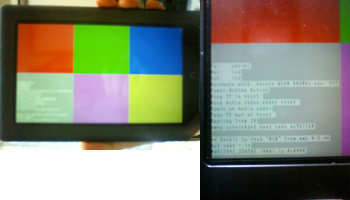
\includegraphics[width=1\hsize]{image2012-gum/u-boot-nook.png}
  \end{center}
  \caption{U-Bootが起動している様子}
  \label{fig:u-boot-booting}
\end{figure}

なお、ここで紹介するU-Bootの改造は、まだ不十分なため、続くuImageをmini-SDから
ロードしてカーネルを実際に立ち上げるところまでは出来ていません。しかしながら、
U-Bootのprintf()に記載した結果はLCDに出力できているので、こちらを
元にU-Bootの改造を続ける事ができそうです。

\subsection{終わりに}

今回ブートローダであるU-Bootを使い、Debian上でクロスコンパイル環境を作って
実際にU-Bootが起動するまで試してみました。PCほどにはBIOSも無い、デバッグ用ポートも無い
実環境で、大した改造や試行錯誤もなく、いきなりLCDにprintf()出来るのはU-Bootが
よくできている証拠だと思います。また、適当な実環境が無くても、Debianさえあれば
組み込み機対応のハックを欲望のままに試すこともできます。

昨今Android端末の普及のおかげで、ものすごい勢いで巷に「不自由」なソフトウェア環境で
固められたARM CPU搭載の情報端末があふれています。これをきっかけにDebianを使って
これらの端末を「自由」なソフトウェア環境へ変えててみませんか?

\begin{thebibliography}{0}

\bibitem{u-boothistory} 
U-bootdoc 1.2 History,
\url{http://www.denx.de/wiki/view/U-Bootdoc/History}

\bibitem{qemu-u-boot}
Virtual Development Board,
\url{http://www.elinux.org/Virtual_Development_Board}

\bibitem{android-debian} 
東京エリアDebian勉強会2012年4月資料,
\url{http://tokyodebian.alioth.debian.org/pdf/debianmeetingresume201204.pdf}

\bibitem{orig-kernel-nook}
NookColor: Build the Original Kernel,
 \url{http://nookdevs.com/NookColor:_Build_the_Original_Kernel}

\end{thebibliography}

%------------------------------------------------------------------------------
\dancersection{Debian Multiarch Support}{なかおけいすけ}
\label{sec:Multiarch}
%------------------------------------------------------------------------------

\subsection{はじめに}
Debian Multiarch Supportは、同じシステム上で、複数のアーキティクチャーのライブラリやプログラムをインストールおよび実行するしくみです。またエミュレータやcross-build環境も提供されており、amd64とarmelのように大きく異なったアーキティクチャのプログラムも動かすことができます。

たとえば64bitのマシンで、あるプログラムを動かしたいのに32bit版しかないことがあります。multiarchでは、そのプログラムが依存している32bit版のライブラリパッケージをインストールすることができるので、32bit版のプログラムを64bit環境で動かすことができます。
また、x86-64のデスクトップでARMのソフトウェアを開発したいときは、armel版のbuild-dependentライブラリをインストールすれば、x86-64のデスクトップで開発することができますし、qemuを使えば、テストすることもできます。

ただ注意しなければいけないのは、複数のアーキティクチャが共存できるのは**ライブラリパッケージだけ**で、**プログラムは共存できない**ということです。


%%%%%%%%%%%%%%%%%%%%%%%%%%%%%%%%%%%%%%%%%%%%%%%%%%%%%%%%%%
%% HOW TO USE MULTIARCH?
%%%%%%%%%%%%%%%%%%%%%%%%%%%%%%%%%%%%%%%%%%%%%%%%%%%%%%%%%%


\subsection{つかいかた}
Multiarchを使うには、インストールしたい他のアーキティクチャを指定します。これをセカンドアーキティクチャと呼びます。セカンドアーキティクチャを指定した後、必ずパッケージデータベースを更新してください。例えばamd64で動いているマシンに、i386のパッケージをインストールしたい場合は以下のようになります。

\begin{commandline}
# dpkg --print-architecture  # どのアーキティクチャーでマシンが動いているか表示
amd64
# dpkg --add-architecture i386 # i386を追加
# dpkg --print-foreign-architectures
i386
# apt-get update # パッケージデータベースを更新
\end{commandline}

ここで、aptitudeコマンドでパッケージのリストを表示すると、パッケージ名の後ろに、:i386と表示されます。たとえばlibc6:i386であれば、i386用のlibc6パッケージという意味です。

\begin{commandline}
$ aptitude search libc6
i   libc6                           - 組込用 GNU C ライブラリ: 共有ライブラリ
p   libc6:i386                      - 組込用 GNU C ライブラリ: 共有ライブラリ
p   libc6-amd64:i386                - 組込用 GNU C ライブラリ: AMD64 用 64 ビッ
p   libc6-dbg                       - 組込用 GNU C ライブラリ: 分離したデバッグ
p   libc6-dbg:i386                  - 組込用 GNU C ライブラリ: 分離したデバッグ
....
\end{commandline}

それでは、i386版のlibc6パッケージをインストールしてみましょう。
他のアーキティクチャーのパッケージをインストールするには、
\begin{commandline}
# apt-get install package:architecture
\end{commandline}

と指定します。よってi386用のlibc6をインストールしたい場合は、以下のようになります。

\begin{commandline}
# apt-get install libc6:i386
\end{commandline}


それでは、i386のプログラムが動くか試してみましょう。i386アーキティクチャで動いているマシンで、以下のプログラムをコンパイルします。
\begin{commandline}
$ uname --machine
i686

$ cat hello.c
#include <stdio.h>
#include <sys/utsname.h>

int main(void)
{
	struct utsname u;
	if(-1 == uname(&u)){
		perror("uname");
		return -1;
	}

	printf("Hello World on %s\n", u.machine);
	return 0;
}

$ gcc -o hello-i686 hello.c

$ file hello-i686
hello-i686: ELF 32-bit LSB executable, Intel 80386, version 1 (SYSV), dynamically linked (uses shared libs),
for GNU/Linux 2.6.18, not stripped

$ ./hello-i686
Hello World on i686
\end{commandline}
%$

32bit ELFのバイナリができて、i386アーキティクチャの上で動くプログラムということがわかります。これを、{\tt libc6:i386}がインストールされたamd64で動いているマシンににコピーして、実行できるか試してみましょう。

\begin{commandline}
$ uname --machine
x86_64

$ ./hello-i686
Hello World on x86_64

$ file hello-i686
hello-i686: ELF 32-bit LSB executable, Intel 80386, version 1 (SYSV), dynamically linked (uses shared libs),
for GNU/Linux 2.6.18, BuildID[sha1]=0x2898c6a77a71f4ae529ae4fb7f91beff44f6762e, not stripped
\end{commandline}
%$
すばらしい。hello-i686は、ELF 32bitバイナリにもかかわらずamd64のマシンでちゃんと動いています。でもなぜこんなことができるのでしょう。

\subsection{Mulit-Arch のしくみ}
Linuxは、実行ファイルフォーマットに、ELF(Executable and Linkable Format)を採用しています。あるプログラムが実行されるとき、まず実行ファイルのヘッダにある、{\tt PT\_INTERP}で指定されているELFインタープリタがロードされます。ELFインタープリタは、プログラムの実行に必要なダイナミックライブラリをロードします。このとき、glibcは、-rpathや、環境変数{\tt LD\_LIBRARY\_PATH}、ハードコードされたディレクトリなどをまわって必要なライブラリを探します。

multiarchは、システム上で利用可能なたくさんのライブラリの中から最適なものを自動的に選択する、このしくみを使って実現されています。すなわち、アーキティクチャ毎に決まったディレクトリにライブラリをインストールして、glibcが検索するディレクトリのリストにそれらのディレクトリを追加しておけば、自動的に必要なライブラリを選んでくれるというわけです。

%ライブラリがインストールされるディレクトリは、以下のとおりです。
%\begin{itemize}
%\item /lib/\$(biarch\_suffix)
%\item /usr/lib/\$(biarch\_suffix)
%\end{itemize}

たとえば、{\tt libc6:i386}パッケージの中身を見てみると、共有ライブラリが{\tt /lib}ではなく、{\tt /lib/i386-linux/gnu}にインストールされていることがわかります。multiarchに対応したライブラリパッケージは、以前のように問答無用で{\tt /lib}や{\tt /usr/lib}に入れるのではなく、{\tt /lib/i386-linux-gnu}や、{\tt /usr/lib/i386-linux-gnu}にインストールされていることがわかります。

\begin{commandline}
$ dpkg -L libc6:i386
/.
/lib/i386-linux-gnu/libnss\_nis-2.13.so
/lib/i386-linux-gnu/libpthread-2.13.so
....(snip)

/etc/ld.so.conf.d
/etc/ld.so.conf.d/i486-linux-gnu.conf
....(snip)

/usr/lib/i386-linux-gnu/gconv/EUC-JISX0213.so
/usr/lib/i386-linux-gnu/gconv/KOI8-T.so
/usr/lib/i386-linux-gnu/gconv/IBM1144.so
....(snip)

/lib/ld-linux.so.2
/lib/i386-linux-gnu/libnss\_nis.so.2
/lib/i386-linux-gnu/libthread_db.so.1
....(snip)
\end{commandline}
%$
先ほどのhello-i686がロードしているライブラリを調べてみると、以下のようになり、
実行時にリンクされる共有ライブラリが、{\tt /lib/i386-linux-gnu}などからロードされていることがわかります。
\begin{commandline}
$ ldd hello-i686
	linux-gate.so.1 =>  (0xf76e3000)
	libc.so.6 => /lib/i386-linux-gnu/i686/cmov/libc.so.6 (0xf756d000)
	/lib/ld-linux.so.2 (0xf76e4000)
\end{commandline}
%$


%%%%%%%%%%%%%%%%%%%%%%%%%%%%%%%%%%%%%%%%%%%%%%
%% HOW TO CONVERT TO MULTIARCHED PACKAGE
%%%%%%%%%%%%%%%%%%%%%%%%%%%%%%%%%%%%%%%%%%%%%%

\subsection{共有ライブラリパッケージを、Multiarch対応にする方法}
\subsubsection{ライブラリをインストールするディレクトリ}
multiarch対応パッケージへの変換方法は、Debian WikiのUsing multiarch\footnote{\url{http://wiki.debian.org/Multiarch/Implementation}}に詳しく述べられています。
Debian Policy (9.1.1)\footnote{\url{http://www.debian.org/doc/debian-policy/ch-opersys.html\#s-fhs}}で、multiarchに関することは共有ライブラリのPATHしか定義されていません。一方で(autoconfのような)ほとんどのアップストリームのビルドシステムは、共有ライブラリや、サポートファイル、(static ライブラリや.soファイルのシンボリックリンクのような)開発に使うファイルを同じターゲットディレクトリにインストールしようとします。Debian Policyはこのようなファイルをすべて、/usr/lib/{\it triplet}サブディレクトリにインストールできるように変更される予定です。
ここで{\it triplet}とは、{\tt dpkg-architecture -qDEB\_HOST\_MULTIARCH}コマンドが返す値のことです。
multiarchでは、ライブラリや実行バイナリをインストールするディレクトリは、このように変更されます。
\begin{commandline}
/usr/lib -> /usr/lib/<triplet>
/usr/lib/<pkgdir> -> /usr/lib/<triplet>/<pkgdir>
/usr/include: no change
/usr/bin: no change
/usr/share: no change
/usr/sbin: no change
\end{commandline}

\subsubsection{パッケージフィールド: Multi-Arch}
multiarchが導入される前は、パッケージの依存関係は、同じアーキティクチャか、すべてのアーキティクチャをサポートしているパッケージを使ってで解決されていました。同じ名前で異なるアーキティクチャのパッケージは当然同時にインストールできないものと扱われていました。multiarchの仕様では、{\tt Multi-Arch}という新しいバイナリパッケージフィールドを追加しました。このフィールドは、{\tt same}、{\tt foreign}、{\tt allowed}の3つの値の1つをとることができます。

{\tt Multi-Arch:same}の時は、同じ名前のパッケージと同じシステムにインストールすることができます(co-installable)が、他のアーキティクチャのあらゆるパッケージの依存を解決することに使ってはならないことを意味しています。また、{\tt Multi-Arch:foreign}の時は、同じ名前のパッケージは同じシステムにインストールすることはできませんが、他のアーキティクチャのパッケージの依存の解決に使うことができます。
つまり、あるライブラリのアーキティクチャーに依存する部分は、{\tt Multi-Arch:same}のフィールドを持つ、{\tt libfoo}というパッケージにして、アーキティクチャに依存しないサポートファイルなどは、{\tt Multi-Arch:foreign}の値を持つ、たとえば{\tt libfoo-data}というパッケージに分離する必要があります。
最後の{\tt Multi-Arch:allow}は、reverse-dependencyがあるパッケージで、同じ名前の他のアーキティクチャのパッケージが依存を解決できるときに指定します。これは、依存しているパッケージのメンテナの仲介なしに、パッケージがアーキティクチャに関係しない依存を持つと、誤って表明することを防ぐためにあります。

\subsubsection{multiarch対応パッケージを作成する手順}
autoconfを使ったupstreamのソースをdhを使って、簡単なパッケージをmultiarchに対応させるときの手順は、このようになるでしょう。
\begin{enumerate}
\item debhelper($>=9$)にBuild-dependさせる
\item {\tt Pre-Depends:\$\{misc:Pre-Depends\}}を追加する
\item {\tt debian/compat}を9にする
\item {\tt debian/*.install}の中の{\tt /usr/lib}を、{\tt /usr/lib/*/}に変更する
\item もし{\tt debian/*.install}や、{\tt debian/*.link}で、{\tt /usr/lib}(またはそのサブディレクトリ)にインストールされるファイルを指定している、もしくはリンクを張るように指定しているなら、{\tt debian/rules}で、{\tt \$(DEB\_HOST\_MULTIARCH)}の値を使うように変更した、これらのファイルを自動生成する必要があるでしょう。
\item {\tt debian/rules}の中に記述されている、{\tt /usr/lib}をすべて{\tt /usr/lib/\$(DEB\_HOST\_MULTIARCH)}に変更する
\item {\tt debian/rules}の中で変数{\tt \$(DEB\_HOST\_MULTIARCH)}を使う必要があるのなら、{\tt debian/rules}の中に、{\tt DEB\_HOST\_MULTIARCH ?= \$(shell dpkg-architecture -dDEB\_HOST\_MULTIARCH)}と記述して、変数{\tt DEB\_HOST\_MULTIARCH}を初期化する。
\item パッケージがビルドできて、共有ライブラリパッケージに、思ったとおりのファイルだけ含まれており、-devパッケージもきちんと動作することを確かめたら、{\tt Multi-Arch: same}と、debian/contorlに記述する。
\item (architecture: all の)commonパッケージが必要なら、{\tt debian/control}で、commonパッケージに、{\tt Multi-Arch:foreign}と設定する。
\end{enumerate}


\subsection{まとめ}
Debian multiarchは、1つのシステムに複数のアーキティクチャのライブラリ、プログラムをインストール、実行するためのしくみです。この文書では、multiarchの使い方と、しくみ、multiarchに対応した共有ライブラリパッケージの作成方法を説明しました。multiarchは、wheezyのRelease Goalです。次期リリースではすべてのひとが、Debian multiarchを使うことができます。

\begin{thebibliography}{8}
\bibitem{spec} MultiarchSpec \url{https://wiki.ubuntu.com/MultiarchSpec}
\bibitem{impl} Multiarch Implementation \url{http://wiki.debian.org/Multiarch/Implementation}
\bibitem{toolchain} Multiarch paths and toolchain implications \url{http://wiki.debian.org/Multiarch/LibraryPathOverview}
\end{thebibliography}


%------------------------------------------------------------------------------
\dancersection{家庭内LANを高速に! - InfiniBand on Debian}{山田 泰資}
\label{sec:ibdebian}
%------------------------------------------------------------------------------

最近のInfiniBand(IB)\cite{IBSPEC}機材の安さに、思わず家庭内IBに
手を出してしまいました。その導入経験を報告します。

\subsection{InfiniBandの特徴と全体像}
最初にIBに触れて戸惑うのは、規定されている範囲がL1-L7と幅広く、
慣れ親しんできたL2:Ethernet、L3:IP、…という階層構造に収まる
単なる「新しいL2規格」ではないことです。また、用語の登場具合が
\begin{screen}
IBのL4にあたる部分にはRC/RD/UC/UD/XRCなどがあります。
RCがTCP、UDがUDPに相当します。IPやMACに対応する要素がGID/LID、
ポートに相当する要素はQPという両端のHCA上に確保されるキュー(WQ)の
組と言えます。そしてWQが1対1対応する形でQPを形成するものがRC/UC、
1対N対応する形のものがRD/UD/XRCという分類になります。SRPなどの
ULPはWQに各種VerbをWQEの形で送り込み、HCAを駆動してRDMAを利用しています。
\end{screen}
などとTLAが分野横断かつ詰め込み気味なのに悩まされます
\footnote{これは各種資料の調子を模して詰め込んでみたサンプルです。セッションでは上記内容は図で解説予定}
。

紙面の関係から詳しくはスライドでとなりますが、資料を読む上では背景として
\begin{itemize}
\item RDMAのためOSバイパスが必要となり、整理・規定範囲がL7まで及ぶこと
\item 既存レイヤへのRDMA導入のため概念+規格+APIと整理が細かくなっていること
\item L2-L3相当の要素にはIB/RoCE/iWARPの三種があり、Verbsで抽象化されること
\end{itemize}
という点までを押さえた上で、同じIBでもどのレイヤ位置の話なのか、
また、本当の意味でIB固有なのかRDMA系各種規格に適用できる話かを
考えながら読み進めると混乱しにくくなります。

\subsection{InfiniBand on Debianの現状}
プロトコルスタックやドライバは素のLinux kernelにも概ね入っているの
ですが、管理ツールなども含めた形ではOFAがOFED(OpenFabrics Enterprise
Distribution)を開発・配布しています。OFEDのLinux版はRedHat向けですが、
実際にはこれを元に各社が移植・独自拡張を行ったものを再配布しており、
有力なものにMellanox社のMLNX\_OFEDパッケージがあります
\footnote{
これの付属マニュアル\cite{MLNXMAN}は何を措いても読むべき資料
}。

DebianではOFED Infiniband Distribution project
\footnote{http://pkg-ofed.alioth.debian.org/}
がドキュメント整備とパッケージングを行っており、squeeze向けには
OFED-1.4.2が、そしてwheezy/sid向けにOFED-1.5のパッケージングが
遅れ気味ですが進んでいます。プロジェクトページには
\begin{commandline}
deb     http://pkg-ofed.alioth.debian.org/apt/ofed-X.Y.Z ./
deb-src http://pkg-ofed.alioth.debian.org/apt/ofed-X.Y.Z ./
\end{commandline}
のapt-lineを追加した上で apt-get install ofed で入るとありますが、
ここには1.4.2までしかないため、現状ではwheezy/sidから先取りするか
自分でビルドします\footnote{以降の説明はsid環境、また、紹介する
機能の関係でLinux 3.4.0ベースとなります}。

今回レベルで使う分にはOFED-1.4で問題ないのですが、例えばIB-FDR
\footnote{IBはシリアルリンクを束ねる方式で、リンク当たり速度を
SDR(2Gbps), DDR(4Gbps), QDR(8Gbps), FDR(14Gbps), EDR(26Gbps), ...と
高速化して帯域を増やします。またリンク数もx1, x4, x12が
規定されています(x4のタイプが主流)}
への対応は1.5.4以降が必要になり、また、さらに新しい機能やカーネルを
使うのであればOFED-3.2や開発中リポジトリ
\footnote{https://beany.openfabrics.org/downloads/MAINTAINERS}
ベースでのリビルドが必要になるなど、試行錯誤が必要です。

\subsection{使ってみよう - 基本的なIB/IPoIB環境の構築}
それでは使ってみましょう。基本的な部分については先のDebianの
プロジェクト資料\cite{DEBIANIB}や各種の日本語記事\cite{ALTIMA}
\cite{ATMARK}もあるため、現在Debianで構築するにあたり固有の
部分だけを紹介します。

\subsubsection{パッケージの導入と初期セットアップ}
プロジェクトのリポジトリであればofedパッケージがあるのですが、
これは現状broken dependencyの状態のため、sidの方より個別に導入します:


\begin{commandline}
# apt-get install opensm ibverbs-utils infiniband-diags perftest                     // 基本ツール群
# apt-get install libmlx4-1 libmthca1 mstflint                                       // HCA関係パッケージ群
# apt-get install ibutils rdmacm-utils rds-tools libsdp1 dapl2-utils                 // 追加ツール群
# apt-get install libibumad-dev libibverbs-dev librdmacm-dev libibcm-dev libdapl-dev // 開発ライブラリ群
\end{commandline}
%$

さて、これでインストールはされましたが、このままでは使えません。
どのようなULP、例えばIPoIBを使うのかどうか、またユーザーランドから
RDMAを叩く使い方をするのかなどは導入ポリシ次第なので、明示的に
有効化する必要があります。

素のOFEDにはこれに使えるinitスクリプト(openibd.conf + openibd)が
入っているのですが、やっていることはモジュールロードとsysctl等の
パラメータ設定なので、以下のモジュールを/etc/moduleに直接ロードして
代えることができます:

\begin{commandline}
# Mellanox HCAベースで構築している今回の場合のモジュールリスト
mlx4_ib ib_mthca ib_uverbs ib_umad ib_ucm rdma_ucm ib_ipoib ib_sdp ib_srp
\end{commandline}
%$

\subsubsection{サブネットマネージャの稼動}
サブネットマネージャ(SM)は系内のトポロジを一元管理し、また
各ポートにGID/LIDを割り当ててActive状態にする上で必須のサービスです。
スイッチに内蔵されていることもありますが、複数起動していても問題ないため
下記の通り起動します:

\begin{commandline}
# cat /etc/defaults/opensm
PORTS=ALL
# /etc/init.d/opensm start
\end{commandline}
%$

後はibstatなどでポート状態がActiveになっていれば、利用可能です。

\subsubsection{チューニングパラメータ}
IPoIBのメリットは通常のLANインタフェースとして利用できることですが、
反面チューニング設定なしではオーバーヘッドが大きく性能が出ません。
Mellanoxのガイドにもありますが、以下の設定はほとんど必須となります:

\begin{commandline}
# echo connected > /sys/class/net/ib1/mode ← RCモードにし、64KB MTU設定を可能にする
# ip link set ib1 mtu 65520                ← 同上
# cat <<EOF > /etc/sysctl.d/network.conf   ← IBへのマッピング効率が向上するよう、バッファを大型化する
net.ipv4.tcp_timestamps = 0
net.ipv4.tcp_sack = 0
net.core.netdev_max_backlog = 250000
net.core.rmem_max = 16777216
net.core.wmem_max = 16777216
net.core.rmem_default = 16777216
net.core.wmem_default = 16777216
net.core.optmem_max = 16777216
net.ipv4.tcp_mem = 16777216 16777216 16777216
net.ipv4.tcp_rmem = 4096 87380 16777216
net.ipv4.tcp_wmem = 4096 65536 16777216
EOF
# sysctl -qp/etc/sysctl.d/network.conf
\end{commandline}
%$

IPアドレスの設定を終えたら、最後に足場の確認としてnetperfや
ib\_read\_bwにて性能を確認しましょう。ほぼワイヤレートが
出せていれば作業は完了です。

\subsection{もっと使ってみよう - SAN構築}
さて、基本的な導通確認は取れたので、次はサーバとしてSANを
構築します。今回はiSCSI over IPoIBとSRPの2通りで行い、比較します。

\subsubsection{iSCSI over IPoIB}
こちらはIPoIBで隠蔽されているので、普通のiSCSI SANの導入と手順は
完全に同じです。今回は
\begin{itemize}
\item target: Linux-iSCSI (LIO)
\item initiator: open-iscsi
\end{itemize}
の組み合わせで構築します。以下が実際のコマンド例です。

\begin{commandline}
# apt-get install targetcli lio-utils ← ターゲット用パッケージを導入
# echo 0 $((2 * 1024 * 1024 * 512)) zero | dmsetup create ramdisk ← 試験用に512GBのダミーディスクを用意
# targetcli
/> cd /backstores/iblock
/backstores/iblock> create ramdisk /dev/mapper/ramdisk ← 先のディスクを登録
...
/backstores/iblock/ramdisk> cd /iscsi
\end{commandline}
%$

\begin{commandline}
/iscsi> create iqn.2003-01.org.linux-iscsi:ramdisk ← IQN生成
...
/iscsi/iqn.20...ramdisk/tpgt1> set attribute authentication=0 ← 認証オフ
Parameter authentication is now '0'.
/iscsi/iqn.20...ramdisk/tpgt1> set attribute generate_node_acls=1 ← アクセス時に自動的にACL許可を生成
Parameter generate_node_acls is now '1'.
/iscsi/iqn.20...ramdisk/tpgt1> set attribute demo_mode_write_protect=0 ← 書込み保護解除
Parameter demo_mode_write_protect is now '0'.
\end{commandline}
%$

\begin{commandline}
/iscsi/iqn.20...ramdisk/tpgt1> cd luns
/iscsi/iqn.20...sk/tpgt1/luns> create /backstores/iblock/ramdisk 0 ← 先のディスクを紐付ける
...
/iscsi/iqn.20...gt1/luns/lun0> cd ../../portals
/iscsi/iqn.20...tpgt1/portals> create 10.254.1.16      ← アクセス用のポータルを開始
...
/iscsi/iqn.20...254.1.16:3260> cd /
/> saveconfig                                          ← 最後に保存
\end{commandline}
%$

淡々とコマンドを打つだけでしたが、以上で設定は完了です。

ターゲット側はこれで稼動を始めたので、次はイニシエータ側です。
open-iscsiデーモン(iscsid)を導入・起動した上で、iscsiadm コマンドで
ターゲット側を照会し、エクスポートされているストレージにアタッチします。

\begin{commandline}
# apt-get install open-iscsi
# /etc/init.d/open-iscsi start                               ← iscsid起動
# iscsiadm -m discovery -t sendtargets -p 10.254.1.16        ← ターゲットIQNを照会する
10.254.1.16:3260,1 iqn.2003-01.org.linux-iscsi:ramdisk
# iscsiadm -m node -T iqn.2003-01.org.linux-iscsi:ramdisk -l ← セッションを確立
...
# iscsiadm -m session                                        ← 認識結果を確認
tcp: [1] 10.254.1.16:3260,1 iqn.2003-01.org.linux-iscsi:ramdisk
# dmesg
...
[ 1403.238057] scsi6 : iSCSI Initiator over TCP/IP
[ 1403.551708] scsi 6:0:0:0: Direct-Access     LIO-ORG  IBLOCK           4.0  PQ: 0 ANSI: 5
...
[ 1404.067053] sd 6:0:0:0: [sde] Attached SCSI disk
\end{commandline}

さて、性能はどんなものでしょうか?

\begin{commandline}
# JOBS=4 OP=write DEV=/dev/sde BS=1m fio bench.ini
...
Run status group 0 (all jobs):
  WRITE: io=6254.0MB, aggrb=210869KB/s, minb=53870KB/s, maxb=54137KB/s, mint=30287msec, maxt=30370msec
\end{commandline}
%$

正直な所、あまり振るいません。さすがに200MB/sでは改善の余地があるとは
思われますが、今回の主眼は次なのでそのままSRPに進みます。

\subsubsection{SRP (SCSI RDMA Protocol)}
さて、次は比較のためRDMA上で直接SCSIを提供するSRPで構築してみます。
\begin{itemize}
\item target: SCST (ib\_srpt)
\item initiator: LIO (ib\_srp) ← カーネル標準のもの
\end{itemize}
の組み合わせで構築します。SRPはターゲット、イニシエータの双方とも
Linux-3.4以降のLIOには含まれていますが、ターゲットについてはSCSTから
コードの取り込み途上で未熟なため、今回はSCSTを使っています。

DebianにはSCSTのパッケージがないため、まずはこれのビルドが必要です
\footnote{
パッケージにしたい所ですが、これをパッケージングする技量が自分にはない…
}
。

\begin{commandline}
$ svn co https://scst.svn.sourceforge.net/svnroot/scst/trunk
$ cd trunk
$ make KDIR=/d/src/linux/master scst iscsi srpt scst_local usr
  ...
  CC [M]  /d/src/scst/trunk/scst/src/scst_main.o
  /d/src/scst/trunk/scst/src/scst_main.c:59:2: warning: #warning
  Patch scst_exec_req_fifo-<kernel-version> was not applied on your kernel.
  Pass-through dev handlers will not work. [-Wcpp]
  ...
make[1]: Leaving directory `/d/src/scst/trunk/usr/fileio'
\end{commandline}
%$

全機能をフルに使うにはカーネルパッチを当てる必要があるという警告が
何件か出ますが、今回の目的には影響しないためこのまま進みます。
最終的に、以下のようなインストール構成になります:

\begin{commandline}
# ls /var/lib/scst/pr/ <- このフォルダがない場合、作成して下さい
# ls /lib/modules/3.4.0-rc1-tai-4f7e834f-next-20120405/extra/scst/
 676 ib_srpt.ko        296 scst_disk.ko        300 scst_tape.ko
3712 iscsi-scst.ko     460 scst_local.ko       620 scst_user.ko
4308 scst.ko           296 scst_modisk.ko      704 scst_vdisk.ko
 292 scst_cdrom.ko     272 scst_processor.ko
 272 scst_changer.ko   272 scst_raid.ko
# ls /usr/local/bin/
132 fileio_tgt*   64 iscsi-scst-adm*  372 iscsi-scstd*  152 scstadmin*
\end{commandline}
%$

それではSCSTでSRP構成を作ってみましょう。iSCSI/LIOの場合は
iSCSI daemonを起動した上で管理コマンドで設定を操作する形でしたが、
SRPの場合はdaemonはおらず、scstadminコマンドでカーネルモジュールの
ロードと設定を行うだけになります。

\begin{commandline}
# echo 0 $((2 * 1024 * 1024 * 512)) zero | dmsetup create zero
# cat > scst-test.conf
# 本ファイルは手動作成してもよいが、scstadminコマンドで構成を作る形でもよい。
# 以降のコメントでは設定エントリに対応するコマンド例を示す。
#
# CMD: scstadmin -open_dev zero -handler vdisk_blockio --attributes filename=/dev/mapper/zero
HANDLER vdisk_blockio {
        DEVICE zero {
                filename /dev/mapper/zero
        }
}
# CMD: scstadmin -add_lun 0 -driver ib_srpt -target ib_srpt_target_0 -device zero
TARGET_DRIVER ib_srpt {
        TARGET ib_srpt_target_0 {
                enabled 1
                rel_tgt_id 2
                LUN 0 zero
        }
}
^D
# modprobe scst
# modprobe scst_vdisk
# modprobe ib_srpt
# scstadmin -config scst-test.conf
\end{commandline}
%$

これでターゲット側は設定完了です。次はイニシエータ側ですが、これは
ibsrpdmコマンドでターゲット側にクエリを投げ、戻ってきたキー情報などを
ib\_srp.koにsysfs経由で受け渡します。

\begin{commandline}
# ibsrpdm -c -d /dev/infiniband/umad1
id_ext=0008f1040399d858,ioc_guid=0008f1040399d858,dgid=fe800000000000000008f1040399d85a,pkey=ffff,service_id=0008f1040399d858
# for i in $(ibsrpdm -c -d /dev/infiniband/umad1); do echo $i > /sys/class/infiniband_srp/srp-mlx4_0-2/add_target; done
# dmesg
...
[1493617.766923] scsi8 : SRP.T10:0008F1040399D858
[1493618.663499] scsi 8:0:0:0: Direct-Access     SCST_BIO zero              300 PQ: 0 ANSI: 5
...
[1493620.678542] sd 8:0:0:0: [sdf] Attached SCSI disk
\end{commandline}
%$

というわけでSRPでも認識できました。起動時に自動的にアタッチさせるには、
上記のibsrpdm出力を/etc/srp\_daemon.confに書き込み、起動時にsrp\_daemonに
同様の処理をさせるようにします。

さて、性能はどうでしょうか?

\begin{commandline}
# JOBS=4 OP=write DEV=/dev/sdf BS=1m fio bench.ini
...
Run status group 0 (all jobs):
  WRITE: io=26387MB, aggrb=898250KB/s, minb=223059KB/s, maxb=233121KB/s, mint=30048msec, maxt=30081msec
\end{commandline}
%$

圧倒的じゃないか、我が軍は・・・という所でしょうか。
ブロックサイズが大きくないと出せない速度なので割り引いて
受け取る必要はありますが、オーバーヘッドの少ないRDMAの威力を
垣間見ることができました。

\begin{thebibliography}{0}
\bibitem{IBSPEC} InfiniBandArchitecture Specification Release 1.2.1, \\
\url{http://members.infinibandta.org/kwspub/specs/register/publicspec/}

\bibitem{MLNXMAN} Mellanox OFED for Linux User Manual, \\
\url{http://www.mellanox.com/related-docs/prod\_software/Mellanox%20OFED%20Linux%20User%20Manual%201\_5\_3-3\_0\_0.pdf}

\bibitem{DEBIANIB} Infiniband HOWTO, \\
\url{http://pkg-ofed.alioth.debian.org/howto/infiniband-howto.html}

\bibitem{ALTIMA} Altima - Mellanox 技術紹介, \\
\url{http://www.altima.co.jp/products/mellanoxtechnologies/mellanox\_techinfo.html}

\bibitem{ATMARK} 松本直人, InfiniBandで変わるデータセンター内通信, \\
\url{http://www.atmarkit.co.jp/fnetwork/tokusyuu/51ib01/01.html} (2011/2), \\
\url{http://www.atmarkit.co.jp/fnetwork/tokusyuu/61ib02/01.html} (2011/7)

% 以下の参考文献は本文中に対応する内容を盛り込みきれなかったためカット

% \bibitem{LINUXIB} Bob Woodruff, Sean Hefty, Roland Dreier, and Hal Rosenstock, Introduction to the InfiniBand Core Software, 2005 \\
\url{http://www.kernel.org/doc/ols/2005/ols2005v2-pages-279-290.pdf}

% \bibitem{ITOHRDMA} 伊藤雅則, プログラマ目線から見たRDMAのメリットとその応用例について, Nov. 2010 \\
% \url{http://www.slideshare.net/thatsdone/rdma}

% \bibitem{IBHIST} Brief History of InfiniBand: Hype to Pragmatism, \\
% \url{https://blogs.oracle.com/RandomDude/entry/history\_hype\_to\_pragmatism}

% \bibitem{RDMAPROG} RDMA Aware Networks Programming User Manual, \\
% \url{http://www.mellanox.com/related-docs/prod\_software/RDMA\_Aware\_Programming\_user\_manual.pdf}

% \bibitem{RSOCKETS} RSockets, \\
% \url{https://beany.openfabrics.org/ofa-documents/presentations/doc\_download/495-rsockets.html}

% \bibitem{GREGORYAPI} Kerr, Gregory. ``Dissecting a Small InfiniBand Application Using the Verbs API.'', 10 May 2011, \\
% \url{http://arxiv.org/abs/1105.1827}

\end{thebibliography}

\clearpage
\newpage

%------------------------------------------------------------------------------
\dancersection{Gentoo/Prefix on Debian}{青田直大}
\label{sec:gentoo}
%------------------------------------------------------------------------------

\subsection{はじめに}

いきなりGentooが出てきて驚かれたかもしれません。ここではDebian下で
Gentoo Prefixをインストールする方法について解説します。

\subsection{Gentoo Prefix}
\subsubsection{Gentooとは}
GentooはDebianやRPMと違ったソースベースのディストリビューションです。
ebuildというパッケージビルド方法や、パッケージの依存関係などを記述した
bashスクリプト風のファイルが
``カテゴリー/パッケージ名/パッケージ名-パッケージバージョン.ebuild''
というファイル名で保管されています。emergeとい
うコマンドはこの 「Portageツリー」というパッケージ情報ファイルツリー
を読んで指定されたパッケージをビルド・インストールするパッケージ管理ソフ
トになっています。

\subsubsection{Prefixサポート}

Gentooも基本的にはLinux上のディストリビューションですが、Debianの
Debian GNU/kFreeBSDと同様にFreeBSD上でのパッケージ管理を目的とした
Gentoo/FreeBSDなどの開発も行なわれています。そういったLinux以外での
Gentooのサポートを総称してGentoo/Altと呼んでいます。
\footnote{\url{http://www.gentoo.org/proj/en/gentoo-alt/}} そのGentoo/Altの中
にGentoo Prefixというものがあります。
\footnote{\url{http://www.gentoo.org/proj/en/gentoo-alt/prefix/index.xml}} こ
れはGentooのシステムを使って(基本的には)他のOS上で、任意のディレクトリ
にパッケージのインストールを行なえるようにするものです。たとえば、Mac
OS X上で動かしてMacPortsやhomebrewの代わりに使ったり、あるいは
FreeBSD上で使ったり、はたまたLinux上で使うことももちろんできます。

\subsection{Gentoo/Prefix on Debian}

さてここからが本題で、このGentoo/PrefixをDebianで使ってみます。おそらく
なんでそんなことを…? と思われるかもしれません。以下のような点があげら
れるかと思います。

\begin{itemize}
\item 非rootユーザでも好きなところにインストールできる
\item Debianにないパッケージをインストールする時に楽できる
\item 技術的に楽しい?
\end{itemize}

Prefixインストールでは好きなディレクトリにインストールできるため、たと
えば自分のホームディレクトリの中などにインストールするようにしてしまえ
ばroot権限がなくともパッケージをインストールすることができます。また、
(もし万が一) Debianにないパッケージがあったとして、それがGentooの方にあ
れば、自分でビルド方法や依存を調べることなく、Gentooのパッケージシステ
ムにおまかせしてしまうことができる、というわけです。

\subsubsection{インストール}

では、さっそくDebian上にインストールしてみましょう。まずはビルドに必要
なパッケージをインストールしておきます。

\begin{commandline}
$ apt-get install bzip2 build-essential bison libreadline-dev libncurses-dev autoconf xz-utils
\end{commandline}

つぎに、Prefixをインストールする場所を決めて、変数EPREFIXに設定し、PATHも通しておきます。

\begin{commandline}
$ export EPREFIX="$HOME/gentoo"
$ export PATH="$EPREFIX/usr/bin:$EPREFIX/bin:$EPREFIX/tmp/usr/bin:$EPREFIX/tmp/bin:/usr/bin:/bin:$PATH"
\end{commandline}

Prefixをインストールするためのスクリプトを取得し、そのスクリプトを使っ
てパッケージ管理ソフトPortageとパッケージ情報のPortageツリーをインス
トールしていきます。

\begin{commandline}
$ wget http://overlays.gentoo.org/proj/alt/browser/trunk/prefix-overlay/scripts/bootstrap-prefix.sh?format=txt \
  -O bootstrap-prefix.sh
$ chmod 755 bootstrap-prefix.sh
$ ./bootstrap-prefix.sh $EPREFIX tree
$ ./bootstrap-prefix.sh $EPREFIX portage
\end{commandline}
%$

この時点でemergeコマンドが使えるようになります。ここからはemergeを使っ
て、Prefix環境を整えていきます。このあたりはあまり今回の主題ではないの
で残りはPrefixのドキュメン
ト\footnote{\url{http://www.gentoo.org/proj/en/gentoo-alt/prefix/bootstrap-solaris.xml}}
を参考にしてください。 \footnote{いまのDebianだとmultiarchの影響でうまく
  動かないところもあるかもしれません…}

\subsection{apt-emerge}

ここまででGentoo/Prefixを解説してきました。しかし、これではあまりに
Gentooすぎますね。Gentoo/Prefixの中にもDebian側で入っているはずのプログ
ラム・ライブラリがインストールされてしまってなんだか無駄なような気がし
てしまいます。特にDebianだとさくさくとバイナリパッケージからインストー
ルされてしまうのに、Gentooだとソースからビルドされて待つのもなかなか大
変なものです。なんとかDebianにあるものはDebianのものを使いつつ、Gentoo
ではどうしても必要なものだけをインストールすることはできないでしょうか。

Gentooではetc/portage/profile/package.providedファイルに以下のように書
くことで、そのパッケージがインストールされていると「見做す」ことができます。

\begin{commandline}
sys-power/acpi-1.6
sys-power/acpid-2.0.16
sys-process/at-3.1.13
sys-devel/autoconf-2.69
sys-devel/automake-1.11.3
app-shells/bash-4.2
\end{commandline}

Debian側にあるパッケージをこうやってGentoo側のパッケージ名にマップして、
package.providedファイルに書くことで、Gentoo側で依存としてパッケージが
ビルド・インストールされることがなくなります。こうして

\begin{enumerate}
\item Gentooのemergeでの依存パッケージを把握
\item Gentooでの依存パッケージ名をDebianのパッケージ名にマップ
\item インストールされたDebianのパッケージ名をGentooのパッケージ名にマップ
\item マップされたパッケージ名をpacakge.providedに追記
\item 再度依存関係を計算しなおして2に戻る
\item これ以上Debianからインストールできなければemergeを開始
\end{enumerate}

といったプロセスを行ない、最小限のパッケージだけで目的のGentooのパッケー
ジをインストールすることができます。この時に肝となるのが、「Gentooでの
  依存パッケージの把握」と「GentooとDebianとのパッケージの相互マップを
  どうするのか」の二点です。

\subsubsection{Gentooでの依存パッケージ}

emergeに対して以下のオプションをつけて出力を解析します。

\begin{itemize}
\item -p (--pretend): インストールを実行せずインストールパッケージ一覧だけを出力します
\item -q (--quiet): 無駄な情報を出力しないようにします
\item -t (--tree): インストールするパッケージを依存関係のツリー状に出力します
\end{itemize}

-tが一番重要なところです。これを指定することでこのようにツリー状に出力されます。

\begin{commandline}
$  emerge -pqt --quiet-repo-display chromium
[ebuild  N    ] www-client/chromium-20.0.1132.21
...
[nomerge      ] www-client/chromium-20.0.1132.21
[ebuild  N    ]  dev-libs/nss-3.13.4
[ebuild  N    ]   dev-libs/nspr-4.9
[ebuild  N    ]    sys-devel/autoconf-2.13
[ebuild  N    ]     sys-devel/autoconf-wrapper-12
[ebuild  N    ]   dev-db/sqlite-3.7.12.1
...
\end{commandline}

このツリーの浅いところからDebianのパッケージへとマップしていきます。浅
いところからマップしていくことで、できるだけ多くの依存解決をDebian側に
おまかせします。つまり、たとえばここで dev-libs/nsprをDebian側でインス
トールすることに成功すればこのツリーを

\begin{commandline}
[ebuild  N    ] www-client/chromium-20.0.1132.21
...
[nomerge      ] www-client/chromium-20.0.1132.21
[ebuild  N    ]  dev-libs/nss-3.13.4
[ebuild  N    ]   dev-db/sqlite-3.7.12.1
...
\end{commandline}

ここまで一気に縮小することができるというわけです。

\subsubsection{GentooからDebianへのマップ}

Gentooのパッケージ名からDebianのパッケージ名へのマッピングを行ないます。
Gentooのパッケージ名にはカテゴリがついていますが、Debianの方にはそれが
ないので、とりあえず外してしまいます。そして、以下の順番で探索をかけます。

\begin{itemize}
\item libパッケージ名-dev
\item パッケージ名-dev
\item パッケージ名
\end{itemize}

Gentooのパッケージでは一般にDebianの*-devに入るようなものがインストール
されているので、*-devを優先してインストールするようにしています。

また、dev-rubyカテゴリのものにはruby-をパッケージ名につけるなどの工夫を
したり、どうしてもこれでマップできないものは明示的にマッピングを書くな
どの対処もしています。

\subsubsection{DebianからGentooへのマップ}

こうしてDebianへとパッケージをインストールできたら、インストールできた
パッケージのバージョンを取得してGentooのパッケージ名へのマップをしてい
きます。これは単純に\texttt{dpkg -l ...}の結果を使うだけですね。
現状Debianの仮想
パッケージから選択される実際のパッケージのバージョンをとれず、うまくマッ
プできていません…。

\subsubsection{実行サンプル}

これらのアイデアを実装したのが\texttt{apt-emerge}スクリプトになります。このスク
リプトは基本的に上記のemergeが使えるようになった段階で使えるようになっ
ていますが、一部のパッケージはGentooのコア部分に大きく食いこんでいるの
でそれらはGentooで入れておかないといけません。また、Debianのmultiarchに
対応するようにCFLAGS/LDFLAGSを調整します。

\begin{commandline}
$ vi $EPREFIX/etc/make.conf
CFLAGS="-O2 -I/usr/include/x86_64-linux-gnu"
LDFLAGS="${LDFLAGS} -L/usr/lib/x86_64-linux-gnu"
$ FEATURES="-collision-protect" emerge -avg1 --nodeps bash eselect eselect-python python portage libffi
\end{commandline}
%$

これでapt-emergeが動くようになるはずです。\texttt{apt-emerge}を動かすと自動的に必要なパッケージをapt-getに渡し、可能な限りの依存を解決してから、emergeに処理を渡します。

例としてTwitterクライアント
mikutter\footnote{http://mikutter.hachune.net}をapt-emergeでインストー
ルしてみましょう。これはRubyとRuby/Gtk2などを使ったパッケージなので、普
通にemergeするだけであれば、gtkなど大量にビルドされるはずです
が……\texttt{apt-emerge mikutter}後にGentoo側になにがインストールされているかを
リストアップしてみましょう(仮想パッケージは除いてあります)。

\begin{commandline}
$ eix -I -c |grep -v virtual
[I] app-admin/eselect (1.3.1@06/03/2012): Gentoo's multi-purpose configuration and management tool
[I] app-admin/eselect-python (20111108@06/03/2012): Eselect module for management of multiple Python versions
[I] app-admin/python-updater (0.10-r2@06/04/2012): Script used to reinstall Python packages after changing of active Python versions
[U] app-shells/bash (4.2_p28@06/03/2012 -> 4.2_p29): The standard GNU Bourne again shell
[I] app-shells/push (1.5@06/04/2012): A POSIX shell function to treat a variable like an array, quoting args.
[I] dev-lang/python (2.7.3-r2(2.7)@06/04/2012): Python is an interpreted, interactive, object-oriented programming language.
[I] dev-libs/libffi (3.0.11@06/04/2012): a portable, high level programming interface to various calling conventions.
[I] net-misc/mikutter (9999@06/04/2012): mikutter is simple, powerful and moeful twitter client
[I] sys-apps/baselayout-prefix (1.12.14@06/04/2012): Baselayout for Gentoo Prefix installs
[I] sys-apps/portage (2.2.01.20430@06/04/2012): Prefix branch of the Portage Package Manager, used in Gentoo Prefix
[I] sys-apps/tcp-wrappers (7.6.22@06/04/2012): TCP Wrappers
[I] sys-devel/gnuconfig (20120116@06/04/2012): Updated config.sub and config.guess file from GNU
\end{commandline}
%$

ご覧のように10個程度しかGentoo側にはインストールされていませんが、
mikutter-9999 (SVN trunkのバージョン)がしっかりとインストールされています。

\subsection{これから}

apt-emergeのスクリプトはまだコンセプトが実装されただけで、いろんな部分
がad-hocになっています。よりDebianのパッケージ名とGentooのパッケージ名
とのマッピングの推測を賢くしたり、必要な固定マップデータを拡充し、
Debianのvirtualパッケージをうまく処理したりするなど、より使いやすいビル
ドシステムを作れればと思います。自分自身Debianに深く知識を持っているわ
けではないので、もしかするともっと効率のよい実装もあるかもしれません…。
もし興味を持っていただければ、開発参加・アドバイスしていただけましたら
幸いです。


%------------------------------------------------------------------------------
\dancersection{Debianでもマルチタッチデバイスを使う}{赤部 晃一}
\label{sec:multitouch}
%------------------------------------------------------------------------------

\subsection{はじめに}

近年、スマートフォンやタブレット端末などのマルチタッチスクリーンを搭載したデバイスが、あらゆる場面で注目を集めています。この社会情勢を受け、派生ディストリビューションのUbuntuでは、バージョン10.10以降でタッチデバイス向けのアプリケーションの開発をサポートするuTouchが提供されるようになりました。今年の4月には、Debianにおいてもタッチデバイスのサポートが強化されたGTK+3.4やX server 1.12が提供されるようになり、今後Linuxデスクトップにおいてもマルチタッチ操作対応のアプリケーションが増えることが期待されます。\footnote{筆者は期待されますと言いましたが、デスクトップ環境では未だにマウス操作が主流であり、タッチアプリの普及にはまだまだ時間がかかりそうです。ちなみに筆者はマウスをほとんど使わずに、ペンタブレットをマウスの如く常用しています。}

ここでは、まずUbuntuのuTouchを紹介し、DebianにuTouchを導入します。次に、ginnというソフトウェアを用いることで、タッチ操作に対応していないソフトウェアでもタッチ入力ができるようにします。

\subsection{uTouchの概要}

\subsubsection{uTouchの目的}

uTouchは、アプリケーションにおけるタッチ入力処理をサポートするためのフレームワークです。例えば、GTK+で開発中のアプリケーションを、2本の指を使った回転操作に対応させる場合を考えます。GTK+3.4に搭載されたタッチイベントを使って実装させる場合、タッチしている指の本数や、それぞれの指の動きなどを全てトレースし、指同士の位置関係や相対速度を計算した上で、それが2本指による回転操作である事を判定させる処理を記述する必要があります。しかしそれは言葉通り労力のかかる作業であり、複数のジェスチャー(タップ、スワイプ、ピンチ、回転など)について一つずつ記述していてはキリがありません。

そこで登場するライブラリーがuTouchです。uTouchはいくつかのタッチジェスチャーを自動的に認識し、それぞれのジェスチャーについてイベントを発生させるため、マルチタッチ操作対応のアプリケーションを作成するときの工数を大幅に減らすことができます。

Ubuntu標準のデスクトップインターフェイスであるUnityでは、3本指ドラッグでウィンドウの移動、4本指タップでメインメニューの表示ができます。\footnote{対応しているジェスチャーはUbuntu Wikiで調べられます。\url{https://wiki.ubuntu.com/Multitouch\#Supported_Gestures}}

\subsubsection{uTouch周りの依存関係}

\begin{figure}[ht]
  \begin{center}
    \includegraphics[width=0.4\hsize]{image2012-gum/utouch-depends.eps}
  \end{center}
  \caption{uTouch周りの依存関係}
  \label{fig:image01}
\end{figure}

図\ref{fig:image01}にuTouch周りの依存関係を示します。上のパッケージが下のパッケージに依存しており、太枠の部分がuTouchの基幹のパッケージです。まずutouch-evemuによって、デバイス毎に異なるフォーマットのタッチデータを一つの決まったフォーマットに変換し、イベントデバイスをエミュレートすることで変換結果を出力します。次にutouch-frameによってutouch-evemuが出力する情報を扱いやすい形に変換します。このタッチデータを元にutouch-grailがジェスチャーを認識します。最後にXサーバーの拡張機能として動作するutouch-geisによって、ジェスチャー情報がイベントなどの形でアプリケーションに提供されます。

GTK+やQtを使ったアプリケーションでタッチジェスチャーを利用する場合、通常はutouch-geisをそのまま使うのではなく、GUIツールキット向けのライブラリーを用います。GTK+の場合はlibgrip、Qtの場合はutouch-qmlです。今回扱うginnは、タッチジェスチャーがサポートされていないソフトウェア	を、タッチ操作できるようにするためのソフトウェアです。

\subsection{uTouchをDebianに取り込む}

\subsubsection{dgetを使ったソースパッケージのダウンロード}

では早速、uTouchをDebianに取り込んでみましょう。まず、dgetコマンドを使ってlaunchpadからUbuntuに含まれているソースパッケージをダウンロードします。私の場合はuTouchのメンテナーへのtrust pathが無いので、\texttt{dget}に\texttt{-u}オプションを付け、サインの確認を省略します。以下のURLはlaunchpadのサイトで取得できます。\footnote{例えばutouch-evemuのdscファイルの場所は次で調べられます: \url{https://launchpad.net/ubuntu/+source/utouch-evemu}}

\begin{commandline}
$ dget -u https://launchpad.net/ubuntu/+archive/primary/+files/utouch-evemu_1.0.9-0ubuntu1.dsc
$ dget -u https://launchpad.net/ubuntu/+archive/primary/+files/utouch-frame_2.2.3-0ubuntu1.dsc
$ dget -u https://launchpad.net/ubuntu/+archive/primary/+files/utouch-grail_3.0.5-0ubuntu1.dsc
$ dget -u https://launchpad.net/ubuntu/+archive/primary/+files/utouch-geis_2.2.9-0ubuntu2.dsc
\end{commandline}

\subsubsection{パッケージの修正・ビルド}

まずは次のコマンドを実行し、ビルドに必要なパッケージをインストールしておきます。

\begin{commandline}
$ sudo apt-get install libx11-xcb-dev xmlto libxi-dev xcb-proto python-xcbgen python-dev \
   dh-autoreconf doxygen asciidoc docbook-xsl libdbus-1-dev xserver-xorg-dev
\end{commandline}
%$

前節でダウンロードしたソースパッケージのうち、utouch-geisはそのままではビルドできないため、パッケージに変更を加える必要があります。まず、utouch-geis-2.2.9/configure.acの次の箇所を変更します。

\begin{commandline}
PKG_CHECK_MODULES([XI2], [x11 xext xi >= 1.3], ,
		  AC_MSG_ERROR([XI2 development libraries not found]))
PKG_CHECK_MODULES([PYTHON], [python >= 2.7]) # ←この行

AX_ENABLE_XI2
\end{commandline}

Debianでは、python.pcではなくpython-2.7.pcを参照する必要があるため、次のように変更します。

\begin{commandline}
PKG_CHECK_MODULES([PYTHON], [python-2.7])
\end{commandline}

パッチを作成する方法はいくつかありますが、ここでは\texttt{dpkg-source}コマンドを利用します。ファイルを修正後、次のコマンドを実行するとパッチが作成されます。

\begin{commandline}
$ cd utouch-geis-2.2.9
$ dpkg-source --commit

dpkg-source: info: local changes detected, the modified files are:
 utouch-geis-2.2.9/configure.ac
Enter the desired patch name: 01_fix-pkg-config-path.patch
\end{commandline}
%$

パッチ名を入力して確定すると、パッチ編集画面に移ります。パッチの説明等を入力して保存してください。

それでは、パッケージのビルドです。依存関係上、図\ref{fig:image01}の下のパッケージから順にビルド・インストールします。ダウンロードしたパッケージに含まれているdebian/controlのMaintainerフィールドを自分の名前に変更し、dchコマンドでバージョン番号を修正し、\texttt{debuild}コマンドを実行してバイナリパッケージを作成します。例えばutouch-evemuの場合は次のコマンドを実行します。

\begin{commandline}
$ cd utouch-evemu-1.0.9
$ dch -v 1.0.9-1~dgm1 -D unstable // Debianバージョンを若干上げておく (abbrev of Debian Grand Meeting)
$ debuild -uc -us // サイン省略
\end{commandline}
%$

いくつかのパッケージでは、ビルド後にLintianの警告が表示されます。本来は警告が消えるまで修正したいところですが、ここでは割愛します。

\subsection{実際にuTouchを使ってみる}

\subsubsection{2本指・3本指ジェスチャーの有効化}

まず次のコマンドを実行し、タッチ入力をuTouchが認識しているかどうか確認します。

\begin{commandline}
$ utouch-frame-test-x11
\end{commandline}
%$

このコマンドを実行した状態で、タッチデバイスを4本以上の指で触ると、画面が動くはずです。しかし、3本指以下では反応しません。この理由は、2本指や3本指のジェスチャーは、右クリックやスクロールなどのシステムの別の設定と競合してしまうためです。uTouchでこれらのジェスチャーを認識させたい場合は、xinputコマンドで設定を無効化させる必要があります。

まず、\texttt{xinput}コマンドを使って接続されているタッチデバイスのIDを確認します。下は筆者の環境で\texttt{xinput list}コマンドを実行した結果です。

\begin{commandline}
$ xinput list
+ Virtual core pointer                    	id=2    [master pointer  (3)]
|   → Virtual core XTEST pointer              	id=4    [slave  pointer  (2)]
|   → HID 0566:3107                           	id=11   [slave  pointer  (2)]
|   → Wacom Bamboo 16FG 4x5 Finger            	id=8    [slave  pointer  (2)]
|   → Wacom Bamboo 16FG 4x5 Pen stylus        	id=9    [slave  pointer  (2)]
|   → Wacom Bamboo 16FG 4x5 Pen eraser        	id=12   [slave  pointer  (2)]
+ Virtual core keyboard                   	id=3    [master keyboard (2)]
    → Virtual core XTEST keyboard             	id=5    [slave  keyboard (3)]
    → Power Button                            	id=6    [slave  keyboard (3)]
    → Power Button                            	id=7    [slave  keyboard (3)]
    → HID 0566:3107                           	id=10   [slave  keyboard (3)]
\end{commandline}
%$

筆者が使用しているタッチデバイスは「Wacom Bamboo 16FG 4x5 Finger」に相当するので、IDは8であることが分かります。

ここで以下の3つのコマンドを実行すると、システムの2本指・3本指に対する設定が無効化されます。\footnote{設定方法の詳細はUbuntu Wikiで調べられます。\url{https://wiki.ubuntu.com/Multitouch/TouchpadSupport}}

\begin{commandline}
$ xinput set-prop 8 "Synaptics Tap Action" 0 0 0 0 1 0 0
$ xinput set-prop 8 "Synaptics Two-Finger Scrolling" 0 0
$ xinput set-prop 8 "Synaptics Click Action" 1 0 0
\end{commandline}
%$

設定を変更したら、もう一度utouch-frame-test-x11コマンドを実行してみましょう。2本指や3本指でタッチした場合も画面が動くようになるはずです。

この設定は、デバイスを抜き挿ししたり、ログイン・ログアウトする度にリセットされてしまいます。ログイン時に次のようなスクリプトが実行されるようにしておくと、自動的に設定できます。\footnote{諸事情により、スクリプト中の文字を一部変更して表示しています。右矢印「→」は、正しくは折れ矢印(U+21B3)です。}

\begin{commandline}
#!/bin/sh
devname="Wacom Bamboo 16FG 4x5 Finger" # xinput list で調べた名前
devid=$(xinput list | tr -d "\\012" | sed -e "s/.*→\\s$devname\\s\\+id=\\([0-9]\\+\\).*/\\1/g")
xinput set-prop $devid "Synaptics Tap Action" 0 0 0 0 1 0 0
xinput set-prop $devid "Synaptics Two-Finger Scrolling" 0 0
xinput set-prop $devid "Synaptics Click Action" 1 0 0
\end{commandline}
%$

\subsubsection{ginnを利用したタッチ操作}

2012年6月現在、uTouchを利用したアプリケーションが非常に少なく\footnote{Ubuntuのリポジトリーでutouchに依存するパッケージを検索しても、unityインターフェイスや、eog、evince等のごく一部のアプリケーションしかヒットしません。}、さらにGTK+向けのライブラリーであるlibgripが、筆者が使用しているWacom Bamboo CTH-460に対して機能しない状況です\footnote{詳しい原因は分かりませんが、Ubuntu 11.10以前は動作していました。}。本来であれば、アプリケーションをコードレベルでマルチタッチに対応させたいところですが、今回は唯一動作確認できたginnというソフトウェアを利用します。

ginnは、utouch-geisによって取得したタッチイベントに応じて、予め指定したショートカットキーを出力することで、タッチ入力に対応していないアプリケーションをタッチ操作できるようにするソフトウェアです。

まず、先程と同様に\texttt{dget}コマンドでginnをダウンロードし、debian/controlとバージョン番号を修正してビルドします。

\begin{commandline}
$ dget -u https://launchpad.net/ubuntu/+archive/primary/+files/ginn_0.2.4-0ubuntu1.dsc
$ cd ginn-0.2.4
$ editor debian/control # Maintainerを変更
$ dch -v 0.2.4-1~dgm1 -D unstable
$ debuild -uc -us
\end{commandline}
%$

生成されたパッケージをインストールしてginnコマンドを実行し、タッチデバイスを何本かの指で撫でてみてください。画面が動き、タッチジェスチャーの種類、指の位置などが表示されるはずです。

次に、Ubuntu向けになっているginnの設定を、Debianに合わせて変更します。まず、ginnの設定ファイルをホームディレクトリー以下にコピーします。

\begin{commandline}
$ cp /etc/ginn/wishes.xml ~/my_ginn.xml
\end{commandline}
%$

コピーした設定ファイルを開いてみましょう。設定ファイルはXML形式となっています。ginnはアクティブウィンドウの種類によって出力するショートカットキーを変更します。ただし、globalタグ以下に記述された設定は、すべてのアクティブウィンドウに対して常に同じショートカットキーを出力します。

例えば、4本指スワイプでGNOME Shellのワークスペースを切り替えるようにするには、設定ファイルを次のように変更します。

\begin{commandline}
<ginn>
  <global>
    <wish gesture="Drag" fingers="4">
      <action name="action1" when="update">
        <trigger prop="delta y" min="5" max="400"/>
        <key modifier1="Control_L" modifier2="Alt_L">Down</key>
      </action>
    </wish>
    <wish gesture="Drag" fingers="4">
      <action name="action2" when="update">
        <trigger prop="delta y" min="-400" max="-5"/>
        <key modifier1="Control_L" modifier2="Alt_L">Up</key>
      </action>
    </wish>
  </global>
</ginn>
\end{commandline}
%$

%-------------------------------------------------------
% 大統一ここまで
%-------------------------------------------------------

\newpage
\clearpage

%-------------------------------------------------------

%-------------------------------------------------------------------------------
\dancersection{東京エリアDebian勉強会 2011年の振り返り}{まえだこうへい}
%-------------------------------------------------------------------------------
\index{debianjp@Debian JP}
\index{とうきょうえりあ@東京エリアDebian勉強会}
\index{2011ねん@2011年}

2011年12月で7年目のDebian勉強会が終了しました。

\subsection{基本的な数値}

Debian 勉強会は毎回事前課題事後課題を設定しており、予習復習を必要だと謳っている勉強会です。
実際にどれくらいの人が出席しているのか、またその人たちがどれくらい事前課
題・事後課題を提出しているのか、確認してみましょう。
\fgref{fig:attendandprepostwork}です。
値は一年の移動平均です。

結果を見ると参加者数は下降傾向にあり、事前課題の提出率は昨年からは横ばい傾向です。
事前課題をちゃんとやる常連参加者に収斂されてきているのでしょうか?
一方、事後課題(ブログ)の率はさらに低下しています。昨年、「ブログはもう流行らないのでしょうか」との一言がありましたが、まさにその通りかもしれません。

\begin{figure}[ht]
\begin{center}
 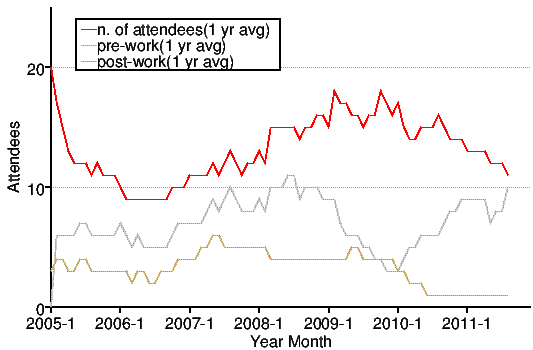
\includegraphics[width=0.7\hsize]{image201112/memberanalysis/attend.png}
\caption{東京エリアDebian勉強会事前課題・事後課題提出実績(12ヶ月移動平均)}\label{fig:attendandprepostwork}
\end{center}
\end{figure}

毎回の参加者の人数と、その際のトピックを見てみます。
今年も昨年同様、人数的には大きく増減はありませんが、10月の筑波大での開催での参加者が、昨年の筑波大でのつくらぐさんとの合同勉強会の時と同じ参加者数でした。新参の参加者を期待した筑波大生の参加は思ったほどではなかった一方、初参加なのにわざわざ都心から筑波大まで参加してくれた方が意外と多かった回でした。2009年から見ると、大学での開催はいつもより参加者数および初参加者が増えるので、来年以降も続けていくと良いでしょう。
また、リストをみると、毎月数名は初参加者も毎月いて、そのうち一部は2回目以降も参加する人がいることを考えると、先ほどの参加数が下降傾向にありつつ、事前課題の提出数が横ばいであるのは、ちゃんと事前課題を提出する人が常連になる傾向にあるのではないか、とも見れます。事前課題の提出率は維持しつつ、参加者数は増やしていく為の対策は必要でしょう。


会場を見ると、今年の会場は、あんさんぶる荻窪以外の公民館などの利用が増えました。
また、今年は3年前の草津温泉、昨年の木更津に続き、三回目のDebian温泉を伊東の山喜温泉で開催しました。
Debian Hack Cafeも6月ごろから月1回程度のペースで再開しているようです。

\begin{table}[ht]
\begin{minipage}{0.5\hsize}
 \caption{東京エリアDebian勉強会参加人数(2005-2006年)}\label{tab:count}
 \begin{center}
  \begin{tabular}{|l|c|p{10em}|}
 \hline
   & 参加人数 & 内容 \\
 \hline
   2005年1月 & 21 & 秘密\\
   2005年2月 & 10 & debhelper 1\\
   2005年3月 & 8 &  (早朝) debhelper 2、social contract\\
   2005年4月 & 6 & debhelper 3\\
   2005年5月 & 8 & DFSG、dpkg-cross、lintian/linda\\
   2005年6月 & 12 & alternatives、d-i\\
   2005年7月 & 12 & toolchain、dpatch\\
   2005年8月 & 7 & Debconf参加報告、ITPからアップロードまで\\
   2005年9月 & 14 & debconf\\
   2005年10月 & 9 & apt-listbugs、バグレポート、debconf翻訳、debbugs\\
   2005年11月 & 8 & DWN翻訳フロー、statoverride\\
   2005年12月 & 8 & 忘年会\\
   2006年1月 & 8 & policy、Debian勉強会でやりたいこと\\
   2006年2月 & 7 & policy、multimedia \\
   2006年3月 & 30 & OSC: debian勉強会、sid \\
   2006年4月 & 15 & policy、\LaTeX{} \\
   2006年5月 & 6 & mexico \\
   2006年6月 & 16 & debconf、cowdancer\\
   2006年7月 & 40 & OSC-Do: MacBook Debian \\
   2006年8月 & 17 & 13執念 \\
   2006年9月 & 12 & 翻訳、Debian-specific、oprofile \\
   2006年10月 & 23 & network、i18n会議、Flash、apt \\
   2006年11月 & 20 & 関西開催: bug、sid、packaging \\
   2006年12月 & 14 & 忘年会 \\
 \hline
  \end{tabular}
 \end{center}
\end{minipage}
\begin{minipage}{0.5\hsize}
 \caption{東京エリアDebian勉強会参加人数(2007-2008年)}\label{tab:count2007}
 \begin{center}
  \begin{tabular}{|l|c|p{10em}|}
 \hline
 & 参加人数 & 内容\\
 \hline
   2007年1月 & 15 & 一年を企画する \\
   2007年2月 & 13 & dbs, dpatch\\
   2007年3月 & 80 & OSC仮想化 \\
   2007年4月 & 19 & quilt, darcs, git\\
   2007年5月 & 23 & etch, pbuilder, superh \\
   2007年6月 & 4 & エジンバラ開催:Debconf7 実況中継 \\
   2007年7月 & 18 & Debconf7 参加報告\\
   2007年8月 & 25 & cdn.debian.or.jp \\
   2007年9月 & 14 & exim \\
   2007年10月 & 30 & OSC Tokyo/Fall(CUPS) \\
   2007年11月 & 19 & live-helper, tomoyo linux kernel patch, server\\
   2007年12月 & 11 & 忘年会\\
   2008年1月 & 23 & 一年を企画する \\
   2008年2/29,3/1 & 36 & OSC  \\
   2008年3月 & 37 & データだけのパッケージ、ライセンス \\
   2008年4月 & 17 & バイナリパッケージ \\
   2008年5月 & 20 & 複数のバイナリパッケージ \\
   2008年6月 & 10 & debhelper \\
   2008年7月 & 17 & Linux kernel patch / module パッケージ \\
   2008年8月 & 10 & Debconf IRC会議とDebian温泉 \\
   2008年9月 & 17 & po4a, 「Debian メンテナのお仕事」 \\
   2008年10月 & 11? & OSC Tokyo/Fall \\
   2008年11月 & 17 & 「その場で勉強会資料を作成しちゃえ」 Debian を使った \LaTeX{} 原稿作成合宿 \\
   2008年12月 & 12 & 忘年会 \\
 \hline
  \end{tabular}
 \end{center}
\end{minipage}
\end{table}

\begin{table}[t]
\begin{minipage}{0.5\hsize}
 \caption{東京エリアDebian勉強会参加人数(2009-2010年)}\label{tab:count2009}
 \begin{center}
  \begin{tabular}{|l|c|p{10em}|}
 \hline
 & 参加人数 & 内容\\
 \hline
   2009年1月 & 12 & 一年を企画する \\
   2009年2月 & 30 & OSC パッケージハンズオン\\
   2009年3月 & 23 & Common Lisp, パッケージ作成 \\
   2009年4月 & 15 & Java Policy, ocaml, 開発ワークフロー\\
   2009年5月 & 13 & MC-MPIパッケージ化、Erlang、Androidアプリ、DDTP \\
   2009年6月 & 14 & DDTP・DDTSS、bsdstatsパッケージ、Debian kFreeBSD\\
   2009年7月 & 4 & スペインにてDebconf 9\\
   2009年8月 & 14 & スペイン Debconf 9 参加報告 \\
   2009年9月 & 26 & GPGキーサインパーティー \\
   2009年10月 & 30 & OSC Tokyo Fall\\
   2009年11月 & 12 & Octave, R, gnuplot, auto-builder \\
   2009年12月 & 10 & 忘年会\\
   2010年1月 & 17 &  東京大学にて新年会 \\
   2010年2月 & 11 & Debian温泉,ocaml,haskell \\
   2010年3月 & 12 & weka,fftw,dpkg v3 quilt \\
   2010年4月 & 15 & upstart,piuparts,debtags \\
   2010年5月 & 22 & 筑波大学,kernel \\
   2010年6月 & 12 & OSC-Doリハーサル  \\
   2010年7月 & 0 & キャンセル  \\
   2010年8月 & 3 & Debconf (NYC) \\
   2010年9月 & 30 & OSC Tokyo/Fall \\
   2010年10月 & 13 & 俺のDebianな一日 \\
   2010年11月 & 15 & ext4,btrfs,nilfs,ceph \\
   2010年12月 & 14 &  cacert, libsane \\
 \hline
  \end{tabular}
 \end{center}
\end{minipage}
\begin{minipage}{0.5\hsize}
 \caption{東京エリアDebian勉強会参加人数(2011年)}\label{tab:count2011}
 \begin{center}
  \begin{tabular}{|l|c|p{10em}|}
 \hline
 & 参加人数 & 内容\\
 \hline
   2011年1月 & 12 & 荻窪,Kinect,アンケートシステム,CACertサイン会 \\
   2011年2月 & 13 & 北新宿生涯学習館,HDFS,Debian Game Team \\
   2011年3月 & ? & OSC Tokyo/Spring,CACert ATE Tokyo \\
   2011年4月 & 12 & IIJ,backports,initramfs,月刊PPC64 \\
   2011年5月 & 15 & 戸山生涯学習館,Apache2モジュール,Debian on ニフクラ,Debian/m68k,月刊PPC64 \\
   2011年6月 & 17 & 東京オリンピックセンター,ドキュメント処理系,2011再計画 \\
   2011年7月 & 3 & DebConf11 \\
   2011年8月 & 12 & 荻窪,パッケージング関連, Debconf11報告 \\
   2011年9月 & 9 & 山喜旅館,Debian温泉2011 \\
   2011年10月 & 22 & 筑波大学,Haskell,LaTeX,レポート自動生成,月刊debhelper開始 \\
   2011年11月 & ? & OSC Tokyo/Fall \\
   2011年12月 & 9 & スクウェア・エニックス,quiltでporting,月刊debhelper,振り返り \\
 \hline
  \end{tabular}
 \end{center}
\end{minipage}
\end{table}

\clearpage

%-------------------------------------------------------------------------------
\dancersection{関西Debian勉強会 2011年の振り返りと2012年の企画}{Debian JP}
%-------------------------------------------------------------------------------
\index{debianjp@Debian JP}
\index{かんさいDebianべんきょうかい@関西Debian勉強会}
\index{2011ねん@2011年}

初回が2007年3月なので、2011年で5年目になりますね。

\subsection{勉強会全体}

毎回のセッションについてですが、
今年はパッケージ作成やBTSに関する題材が多く扱われました。
定番のネタ(Debianの入門的なお話、ライセンス、パッケージ作成、BTS)などの題材は
毎年更新されていくべき題材なので, 今後も繰り返し扱っていきたい所です。
事前課題で提出されていた「インストール大会」のような初心者講習もやってみたい
所ですね。

また、昨年から事前課題の提出が普通になってきましたので、
来年からは事後統計(アンケート)も提出してもらおうか, なんて考えています。

運営に関しては、常連さんだった河田さんが運営側になり、Debian JP Project
へ加入されました。また、今回の発表にある通り倉敷さんが DD になるため
の NM プロセスへ申請されています。

イベント参加については、OSC Kansai@ Kobe, OSC Hokkaido, OSC Kansai@
Kyoto, KOF に参加しました。勉強会から fork した GPG キーサインパーティも
毎回実施されています。今後も継続して参加する予定です。

\subsection{開催実績}

関西Debian勉強会の出席状況を確認してみましょう。グラフで見る
と\fgref{fig:kansaipeoplechart}になります。また、毎回の参加者の人数とその
際のトピックを \tbref{tab:count2011kansai} にまとめました。グラフ中の黒線
は参加人数, 赤線は1年の移動平均です。参加人数が$0$となっているところは人
数が集計されていないor開催されなかった月ですので、欠損値処理をした方が良いですね%
\footnote{R使った事ないので今日は間に合いませんでした}。

Debian勉強会申し込みシステムを使用するようになり, 事前課題を設定すること
も多くなりました。また, アンケートシステムも稼動するようになるでしょうか
ら、今後は事前課題と事後課題のグラフを追加しようと思っています。


\begin{figure}[h]
  \begin{center}
    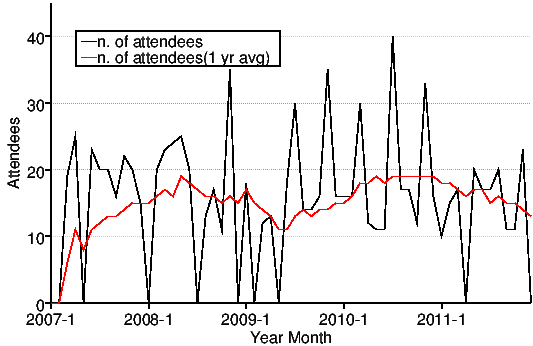
\includegraphics[width=.8\hsize]{image201112/memberanalysis/kansai.png}
  \end{center}
  \caption{関西の参加人数推移(参加人数と12ヶ月移動平均)}
  \label{fig:kansaipeoplechart}
\end{figure}
\begin{table}
  \begin{minipage}{0.5\hsize}
    \caption{関西Debian勉強会の参加人数とトピック(2007年)}
    \begin{center}
      \begin{tabular}{|l|c|p{10em}|}
        \hline
                   & 参加人数 & 内容 \\
        \hline
        2007年3月  & 19       & 開催にあたり \\
        2007年4月  & 25       & goodbye、youtube、プロジェクトトラッカー\\
        2007年6月  & 23       & 社会契約、テーマ、debian/rules、bugreport\\
        2007年7月  & 20前後   & OSC-Kansai \\
        2007年8月  & 20       & Inkscape、patch、dpatch\\
        2007年9月  & 16       & ライブラリ、翻訳、debtorrent\\
        2007年10月 & 22       & 日本語入力、SPAMフィルタ\\
        2007年11月 & 20前後   & KOF \\
        2007年12月 & 15       & 忘年会、iPod touch\\
        \hline
      \end{tabular}
    \end{center}
  \end{minipage}
  \begin{minipage}{0.45\hsize}
    \begin{center}
    \caption{関西Debian勉強会参加人数(2008年)}\label{tab:count2008kansai}
    \vspace{-1em}
      \begin{tabular}{|l|c|p{10em}|}
        \hline
                   & 参加人数 & 内容 \\
        \hline
        2008年2月  & 20       & PC Cluster, GIS, \TeX \\
        2008年3月  & 23       & bug report, developer corner, GPG \\
        2008年4月  & 24       & coLinux, Debian GNU/kFreeBSD, sid \\
        2008年5月  & 25       & ipv6, emacs, ustream.tv\\
        2008年6月  & 20       & pbuilder, hotplug, ssl\\
        2008年8月  & 13       & coLinux \\
        2008年9月  & 17       & debian mentors, ubiquity, DFSG\\
        2008年10月 & 11       & cdbs,cdn.debian.or.jp \\
        2008年11月 & 35       & KOF \\
        2008年12月 & ?        & TeX資料作成ハンズオン\\
        \hline
      \end{tabular}
    \end{center}
  \end{minipage}
\end{table}
\begin{table}
  \begin{minipage}{0.5\hsize}
    \caption{関西Debian勉強会の参加人数とトピック(2009-2010)}
    \begin{center}
      \begin{tabular}{|l|c|p{10em}|}
        \hline
                   & 参加人数 & 内容 \\
        \hline
        2009年1月  & 18       & DMCK, LT \\
        2009年3月  & 12       & Git \\
        2009年4月  & 13       & Installing sid, Mancoosi, keysign \\
        2009年6月  & 18       & Debian Live, bash\\
        2009年7月  & 30?      & OSC2009Kansai \\
        2009年8月  & 14       & DDTSS, lintian \\
        2009年9月  & 14       & reportbug, debian mentors\\
        2009年10月 & 16       & gdb, packaging \\
        2009年11月 & 35       & KOF2009 \\
        2009年12月 & 16       & GPS program, OpenStreetMap \\
        2010年1月  & 16       & Xen, 2010年企画 \\
        2010年2月  & 16       & レンタルサーバでの利用, GAE \\
        2010年3月  & 30?      & OSC2010Kobe \\
        2010年4月  & 12       & デスクトップ環境, 正規表現 \\
        2010年5月  & 11       & ubuntu, squeeze \\
        2010年6月  & 11       & debhelper7, cdbs, puppet \\
        2010年7月  & 40?      & OSC2010Kyoto \\
        2010年8月  & 17       & emdebian, kFreeBSD \\
        2010年9月  & 17       & タイルWM \\
        2010年10月 & 12       & initramfs, debian live \\
        2010年11月 & 33       & KOF2010 \\
        2010年12月 & 14       & Proxmox, annual review \\
        \hline
      \end{tabular}
    \end{center}
  \end{minipage}
  \begin{minipage}{.45\linewidth}
    \caption{関西Debian勉強会の参加人数とトピック(2011)}\label{tab:count2011kansai}
    \begin{center}
      \begin{tabular}{|l|c|p{10em}|}
        \hline
        開催年月  & 参加人数 & 内容 \\
        \hline
        2011年1月 &10        & BTS, Debian GNU/kFreeBSD\\
        2011年2月 &15        & pbuilder, Squeezeリリースパーティ\\
        2011年3月 &17        & ライセンス, Debianのドキュメント関連\\
        2011年4月 &25        & OSC 2011 Kansai @ Kobe, GPG キーサインパーティ \\
        2011年5月 &20        & vi, dpkg \\
        2011年6月 &17        & IPv6, vcs-buildpackage{svn, git}\\
        2011年7月 &17        & OSC 2011 Kansai @ Kyoto, GPG キーサインパーティ\\
        2011年8月 &20        & Debianパッケージ作成ハンズオン\\
        2011年9月 &11        & vcs-buildpackage{bzr, git}\\
        2011年10月&11        & Emacs, vim の拡張のDebianパッケージ, 翻訳\\
        2011年11月&23        & KOF 2011\\
        2011年12月&13        & NMプロセス, BTS\\
        \hline
      \end{tabular}
    \end{center}
  \end{minipage}
\end{table}


\clearpage

%-------------------------------------------------------------------------------
\dancersection{東京エリアDebian勉強会の開催方法}{野島 貴英}
%-------------------------------------------------------------------------------
\index{とうきょうえりあでびあんべんきょうかいのかいさいほうほう@東京エリアDebian勉強会の開催方法}

\subsection{はじめに}

東京エリアDebian勉強会では、毎年12月号資料では勉強会の開催方法についてま
とめています。今回は野島が一通りの流れをまとめます。これを読めば、あなたも
東京エリアDebian勉強会を開けるはず!

\subsection{東京エリアDebian勉強会を開く時のスケジュール}

% 東京エリアDebian勉強会は表\ref{tab:meeting-schedule}のスケジュールで行います。

\begin{table}[ht]
\begin{center}
\small
\begin{tabular}{|p{12em}|p{31em}|}
\hline
時期&作業内容 \\
\hline\hline
開催2ヶ月前 & 場所を確保します。会議室は2ヶ月前に予約しないと埋まりやすいです。\\
\hline
開催2ヶ月前から1ヶ月前 & 勉強会のテーマと、事前課題を決めます。\\
\hline
開催1ヶ月前 & 勉強会のテーマに沿った原稿を募集します。時間枠にあわせた発表が埋まらない場合、
発表者を枠が埋まるまで、探す事になります。また、開催にあたり、作業の分担が必要な時は、この時
ぐらいに割り当てを完了します。また、宴会の場所について、確保が困難な事が予想される場合は、
あらかじめ席のみ予約しておきます。\\
\hline
開催2週間前までに & Debian勉強会予約システム\url{http://debianmeeting.appspot.com}に予約登録
ページを作成します。Debian JP Blog \url{http://www.debian.or.jp/}及び、
Debian勉強会Webサイト \url{http://tokyodebian.alioth.debian.org/} に勉強会の内容を提示します。
メールで debian-users メーリングリストにアナウンスを投げます。
Debian JP twitter や mixi Debian コミュニティーなどにもアナウンスすることが多いです。\\
\hline
開催1週間前 & 発表者は勉強会資料用リポジトリに資料をコミットします。\\
\hline
開催2日前 & 参加者の募集の締切りを行います。この時までに揃った事前課題を勉強会資料にマージします。\\
\hline
開催1日前 & kinkos等の印刷製本サービスに原稿印刷および製本を依頼します。\\
\hline
開催当日 & \begin{enumerate}
  \item 参加者から費用の回収と集計をします。
  \item 勉強会を定刻どおりに開催します。
  \item 司会者、発表者と協力して時間内に勉強会を終了します。
  \item 宴会の場所の確保が困難でない時は、宴会の場所を抑えます。
  \item 宴会の開催、宴会の会計をします。
\end{enumerate} \\
\hline
開催後 & Debian勉強会予約システムからアンケートをおくります。 \\
\hline
12月 & 勉強会のアンケート結果などを一年分集計して発表します。 \\
\hline
\end{tabular}
\caption{全体スケジュール}
\label{tab:meeting-schedule}
\end{center}
\end{table}

\subsection{東京エリアDebian勉強会の開催調整}

東京エリアDebian勉強会の開催調整は専用のメーリングリストがあり、普段はこちらで調整が行われます。
運営者専用のメーリングリストで、一部のコアメンバーのみが参加しています。
運営に積極的に参加したい人は勉強会運営者に連絡を取る必要があります。

\subsection{初めて東京エリアDebian勉強会の開催を担当する場合の事前準備}

初めて東京エリアDebian勉強会の開催を担当する場合以下の項目が準備してあると
スムーズです。

\begin{enumerate}
\item Debian JP Projectの提供するサーバーへログインできるアカウント\\
Debian JP Blogを更新する際に必要になります。
これは通常Debian JP Projectの会員になるときに付与されます。
会員でない人は会員にコミットしてもらうよう依頼する必要があります。

\item \url{http://alioth.debian.org/}アカウント
資料の編集等を行う際に必要になります。
アカウントを取得したら、メーリングリストでtokyodebianグループ権限に所属させてほしい旨、
取得したアカウント名を沿えて依頼します。このアカウントは誰でも取得可能です。

\end{enumerate}

また、勉強会の幹事担当の場合に必要な知識とコンピュータの環境は以下になります。

\begin{enumerate}
\item Debianが動作し、インターネットが利用できるPCの用意
\item ssh,emacs,muse-el,git、subversionの基本操作についての知識
\item ブラウザとHTMLの記載の知識
\item \url{http://alioth.debian.org/},\url{http://qwik.jp/}の使い方の知識
\item \LaTeX{}の知識
\end{enumerate}

わからないことや困ったことがあればメールやメーリングリストで聞いてみましょう。

\subsection{東京エリアDebian勉強会の掲示の出し方}

\url{http://www.debian.or.jp/}に掲示を出す場合の編集の仕方は、
\url{http://www.debian.or.jp/project/webmasters.html}にその記載があります。
実際には、subversionでリポジトリをとってきて、\\
\texttt{./www.debian.or.jp/blosxom/ data/events/tokyodebian-XX.d} (XXは第XX回を示します)を
作成します。

\url{http://debianmeeting.appspot.com/eventadmin/edit?eventid=}のフォームの編集
はフォームに沿って情報を入れるだけです。ただ、細かい事は、\url{http://tokyodebian.alioth.debian.org/YYYY-MM.html}へのリンクをURLの
欄に指定し、そちらを参照してもらいます。

\url{http://tokyodebian.alioth.debian.org/}へは、\url{http://qwik.jp/メーリングリスト名}のトップ
ページに記載されているやり方に従います。実際にはgit
で\url{git+ssh://git.debian.org/git/tokyodebian/muse.git} リポジトリをcloneして、muse形式で編集し、make publishする事となります。

\clearpage

%-------------------------------------------------------------------------------
\dancersection{Debian勉強会予約システム再訪}{上川 純一}
%-------------------------------------------------------------------------------
\index{Debianべんきょうかいよやくしすてむ@Debian勉強会予約システム}
\index{python appengine}
\index{django}

Debian 勉強会予約システムの開発開始から2年経ちました。当初は宴会君をリプレー
スするために突貫でつくりあげたものですがほぼそのままの状態で運営されてい
ます。面倒くさがって適当に実装した部分、ウェブアプリケーションで気をつけ
るべきところをよくわからずに書いていた部分があったのでいまから振り返って
どういう課題があったのかを検討します。

\subsection{脆弱性}

\subsubsection{POST/GET の使い分け}

当初めんどくさかったのでpostとgetのハンドラを一緒にしてました。よって、
あらゆるページがGETとPOSTの両方で動くようになっています。それを適切にGET
とPOSTにわけるようにしました。

GETは情報の取得のみ、POSTは登録などの副作用のある処理に利用します。

\index{XMLHttpRequest}
ブラウザのセキュリティモデルとして、same-originじゃないとPOSTがやりにく
いようになっています。GETはたとえばscriptタグやimgタグなどを埋め込んでお
けばいくらでも発行できますが、POSTはXMLHttpRequestの発行が必要で、
XMLHttpRequestにはsame-origin policyがあります。

以前は任意のページからscriptタグの埋め込みをして勝手にDebian勉強会に登録
することが可能でしたが、今はそれができないようになっています。
これは勝手に予約するHTMLページの例です:
\begin{commandline}
<html>
  <head>
    <title>auto reserve exploit</title>
    <script
 src="http://localhost:8080/eventregister?eventid=df24a1e1de11c067c461537dce6394e0e51df6ad
&user_prework=&user_attend=attend&user_enkai_attend=enkai_attend&user_realname=myname">
    </script>
  </head>

  <body>
    <h1>auto reserve exploit</h1>
    <p>
      ぼくはまちちゃん
    </p>
\end{commandline}

\subsubsection{HTML escaping}

当時よくわからなかったのとめんどくさかったので入力文字列のサニタイズとかエスケープとかまったくしてませんでした。関西Debian勉強会ではHTMLタグを勉強会の予約ページの案内文に入力して
いたようで、それでこの脆弱性がそもそも存在するのに思い至りました。

任意の文字列をHTMLとして出力できると、任意のjavascriptのコードを実行する
ことができます。たとえば、説明ページを開いた瞬間に予約登録するイベントを作成することができます。

\begin{commandline}
<script>
var xhr = new XMLHttpRequest();
xhr.open('POST', 'http://localhost:8080/eventregister');
xhr.withCredentials = true
xhr.setRequestHeader('Content-Type', 'application/x-www-form-urlencoded');
xhr.send('eventid=df24a1e1de11c067c461537dce6394e0e51df6ad&'
+ 'user_prework=%E3%81%BC%E3%81%8F%E3%81%AF%E3%81%BE%E3%81%A1%E3%81%A1%E3%82%83%E3%82%93&'
+ 'user_attend=attend&user_enkai_attend=enkai_attend&user_realname=hamachi');
</script>
\end{commandline}

\begin{wrapfigure}{r}{0.5\hsize}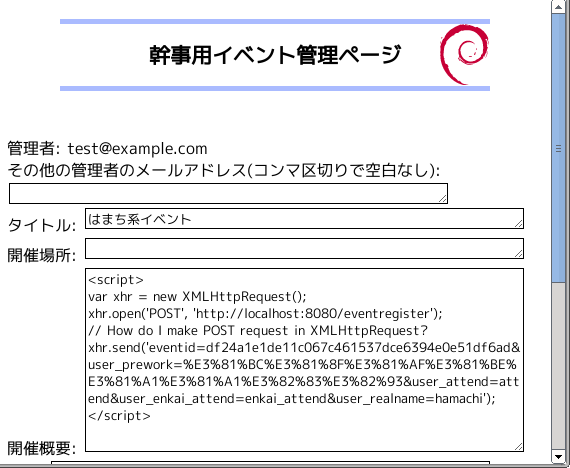
\includegraphics[width=\hsize]{image201201/xhr.png}\end{wrapfigure}

しかたがないので文字列をエスケープするようにしました。
副作用としてHTMLタグを説明文に打ち込むことができないようになっています。

\subsubsection{任意のURL表示}

Debian勉強会予約システムでは説明文の表示が貧弱な代わりに任意のURLを
iframeで埋め込み表示できるようにしています。通常管理している勉強会のWiki
ページを埋め込むことで二重に情報を管理しなくてすむようにという意図です。

URLの中には特殊なものもあります。\url{javascript:}で始まるURLだとその
Javascriptのコードを実行することができます。できても普通の役には立たなさ
そうなので\url{http://}以外は許可しないようにしておきました。

また、iframe buster と呼ばれる手法によりiframe
から脱出できるようで、そういうページをiframeの中でひらいているつもりにな
るとユーザが誤解する可能性があります。

\index{iframe sandbox}
すべてのブラウザでサポートされているわけではないのですが、iframeに
sandbox属性をつけておきjavascriptなどの実行を制約しておきました。

\subsection{可能性と脆弱性のバランス}

今回いろいろと脆弱性があったのでふさいでみました。しかし、脆弱性を塞ぐの
も、ありうる被害とのバランスで考えるべきだと思います。Debian勉強会に提出
する事前課題が漏洩する、勝手に宴会に参加することになっている等の程度の脆
弱性と、自由にHTMLが記述できる自由とどちらが重要かと考えてみてください。
すこし悩ましいと思いませんか?

\clearpage

%-------------------------------------------------------------------------------
\dancersection{quiltでportingしてみた}{杉本典充}
%-------------------------------------------------------------------------------
\index{quiltでぽーてぃんぐしてみた@quiltでportingしてみた}
\index{porting}
\index{kFreeBSD}

\subsection{はじめに}

debianのパッケージ作成で使用しているパッチ管理ツールquiltについて説明します。
またquiltを用いてkFreeBSDのportingパッチを作成しましたので、これについても説明します。

\subsection{Debianパッケージのフォーマット}

現在Debianで使用している主なソースパッケージフォーマットは2つです。
\footnote{東京エリアDebian勉強会 2010年03月号「dpkg ソース形式 "3.0(quilt)"」 吉野与志仁}
\footnote{\url{http://wiki.debian.org/Projects/DebSrc3.0}}

\begin{itemize}
 \item{3.0(native):tarball1つで構成されたソースパッケージフォーマット}
  \begin{itemize}
   \item{packagename-version.tar.ext}
   \item{packagename-version.dsc}
  \end{itemize}
  \item{3.0(quilt):あるアップストリームのtarballとDebianパッケージ作成に
必要なtarballに分割しているソースパッケージフォーマット}
  \begin{itemize}
   \item{packagename-upstreamversion.orig.tar.ext}
   \item{packagename-upstreamversion.orig-component.tar.ext(任意)}
   \item{packagename-debianversion.debian.tar.ext}
   \item{packagename-debianversion.dsc}
  \end{itemize}
\end{itemize}

ソースパッケージフォーマットの詳細は `dpkg-source(1)' コマンドで確認することができます。
\footnote{manによると3.0(custom)、3.0(git)、3.0(bzr)というパッケージ形式の定義があるようです。}

アップストリームのソースコードを無修正のままDebianパッケージを作成した場合、
lintian処理でエラーになったり、Debianの開発ポリシーを満たせない場合が
あります(アップストリームのソースコードはIPv6で動作しない、など)。
そのときは、3.0(quilt)のソースパッケージフォーマットでパッケージを作成し、
必要なパッチを当ててからソフトウェアのビルド処理を行うことで対応させます。

\subsection{quiltパッケージ}
quiltはdebianパッケージを作成するときにパッチファイルを管理するツールとして
採用しているソフトウェアです。
Debianパッケージとして提供しており、aptでインストールできます。

\begin{commandline}
# apt-get update
# apt-get install quilt
\end{commandline}

quiltコマンドは複数のpatchファイルをスタックに積んだようなイメージで、
パッチの適用順番を管理します。
\footnote{東京エリアDebian勉強会 2007年01月号「パッチ管理ツールquiltの使い方」小林儀匡}
quiltコマンドを使うことで、パッケージ作成に必要なパッチが複数ある場合も
正しく適用でき、不要なパッチが出てきたときにそのパッチを取り除くことが容易に
なります。


\subsection{quiltの使用例:Debian GNU/kFreeBSD向けのportingパッチ作成}

\subsubsection{Debian GNU/kFreeBSDとは}
Debian Projectで開発しているOSはLinuxカーネルを用いた「Debian GNU/Linux」が有名ですが、
Linuxカーネル以外を用いたDebianがあります。その1つとしてFreeBSDカーネルを用いた「Debian GNU/kFreeBSD」
\footnote{\url{http://wiki.debian.org/Debian\_GNU/kFreeBSD}}があり、ユーザランドはDebianなので APT が使え、
デバイスやシステムコールといったカーネル特有の機能はFreeBSDカーネルに準じる、という特徴があります。
Debuan GNU/kFreeBSDは安定版のリリースには至っていませんが、日々開発が続けられています。
本稿では以降「Debian GNU/kFreeBSD」を「kfreebsd」と略記します。

\subsubsection{kfreebsdのporting作法}
Debianのporting関連情報およびkfreebsdのporting情報は以下にあります。

\begin{itemize}
 \item{\url{http://www.debian.org/ports/}}
 \item{\url{http://www.debian.org/ports/kfreebsd-gnu/}}
 \item{\url{http://glibc-bsd.alioth.debian.org/porting/}}
\end{itemize}

「\url{http://glibc-bsd.alioth.debian.org/porting/PORTING}」を読むと
kfreebsd向けにportingするには以下の確認および修正が行うようにとあります。

\begin{itemize}
 \item{Add our system name to checks here and there}
  \begin{itemize}
   \item{Makefileやスクリプト中のunameなどをチェックしてください。 }
  \end{itemize}
 \item{debian/control files}
  \begin{itemize}
   \item{debian/controlファイルでArchitectureをlinux専用ソフトウェアの場合は「linux-any」等、
CPUの違いのみでLinux、kfreebsdは関係なく使用できるソフトウェアの場合は「any-i386」等に変更してください。}
  \end{itemize}
 \item{Libraries, your beloved enemy}
  \begin{itemize}
   \item{libtool、aclocal.m4周りに対応してください。}
  \end{itemize}
 \item{Preprocessor Variables}
  \begin{itemize}
   \item{kfreebsdのシステムマクロは「\_\_FreeBSD\_kernel\_\_」、
バージョンマクロは「\_\_FreeBSD\_kernel\_version」なので対応してください。}
  \end{itemize}
 \item{Writing to devfs (kFreeBSD)}
  \begin{itemize}
   \item{FreeBSDカーネルでは(udevではなく)devfsを使うようにしてください。}
  \end{itemize}
 \item{RT signals}
  \begin{itemize}
   \item{FreeBSDカーネルは「POSIX RT (realtime) signals」がないので変更してください。}
  \end{itemize}
 \item{Get libc soname (6 or 6.1 on linux-gnu, 0.1 on kfreebsd-gnu, etc)}
  \begin{itemize}
   \item{使用するlibcの名前をハードコードしているプログラムがあれば修正してください。}
  \end{itemize}
\end{itemize}


\subsubsection{kfreebsdに対応させたいパッケージとその原因}

今回portingするパッケージは既にkfreebsd用パッケージとして存在している
icewmとなります。
icewmはウィンドウマネージャのソフトウェアで軽快な動作をするのが特徴です。
icewmではタスクバーにバッテリー残量アイコンを表示する機能がありますが
kfreebsdでは表示されません。linux-i386及びlinux-amd64では表示されるため
kfreebsdのportingが不完全の可能性があります。

まずはビルド準備とソースコードのダウンロードを行います。

\begin{commandline}
# apt-get update
# apt-get build-dep icewm
$ apt-get source icewm
\end{commandline}
%$

ソースコードを「\_\_FreeBSD\_\_」及び「\_\_linux\_\_」grepすると、電源周りの処理で以下のマクロが検出されます。
\begin{commandline}
$ cd icewm-1.3.7/src
$ grep -nr __FreeBSD__ *
aapm.cc:30:#ifdef __FreeBSD__
aapm.cc:74:#if defined(__FreeBSD__) && defined(i386)
aapm.cc:99:#if defined(__FreeBSD__) && defined(i386)
aapm.cc:273:#ifndef __FreeBSD__
aapm.cc:333:#ifndef __FreeBSD__
aapm.cc:418:#ifndef __FreeBSD__
aapm.cc:463:#ifdef __FreeBSD__
aapm.cc:885:#ifndef __FreeBSD__
aapm.h:2:#if defined(linux) || (defined (__FreeBSD__)) || (defined(__NetBSD__) && defined(i386))
(以下略)
$ grep -nr __linux__ *
(なにもなし)
\end{commandline}
%$

\_\_FreeBSD\_\_マクロはFreeBSD OSを示すマクロですが、kfreebsdでは「\_\_FreeBSD\_kernel\_\_」がシステム(厳密にはカーネル)を示すマクロです。そのためマクロでシステムを切り分けているはずがkfreebsd向けのパッケージビルド時にLinuxカーネル向けの処理が有効なコードとしてビルドされてしまいバッテリー残量アイコンの表示がうまく動作していないようです。

そのため、今回はこのマクロを「PORTING」の記述に従って以下のような修正を行います。

\begin{commandline}
(修正前)#ifdef __FreeBSD__

(修正後)#if defined(__FreeBSD__) || defined(__FreeBSD_kernel__)
\end{commandline}
これで修正方針が定まりましたので、debianパッケージ作成に向けてパッチを作成していきます。

\subsection{quiltの登場}
今回は新規のパッチファイルとなるため、quiltのパッチスタックに新規追加します。
まず、debian/patches/series 記述されておるパッチスタックを見てみます。

\begin{commandline}
$ tail -4 debian/patches/series
tray_hotfixes
imap_unseen
ifstate_exact_check
debian-changes-1.3.7~pre2-1.1
\end{commandline}
%$

次に\texttt{quilt new} を実行し、現在の変更内容を kfreebsd\_porting\_aapm
というファイル名で保存し、スタックに追加します。

\begin{commandline}
$ quilt new kfreebsd_porting_aapm
Patch kfreebsd_porting_aapm is now on top
\end{commandline}

実行下後のパッチスタックは以下のようになります。

\begin{commandline}
$ tail -4 debian/patches/series
imap_unseen
ifstate_exact_check
debian-changes-1.3.7~pre2-1.1
kfreebsd_porting_aapm
\end{commandline}
%$

これでパッチを追加できる準備ができました。
次にportingするために修正を行うソースファイルをquiltで管理するように登録処理をします。
その後「quilt edit ソースファイル」を実行すると、環境変数EDITORで登録したエディタが自
動で起動しますのでソースファイルの修正作業を行います。


\begin{commandline}
$ quilt add src/aapm.h
File src/aapm.h added to patch kfreebsd_porting_aapm
$ quilt edit src/aapm.h
File src/aapm.h is already in patch kfreebsd_porting_aapm
$ quilt refresh
Refreshed patch kfreebsd_porting_aapm
$ quilt add src/aapm.cc
File src/aapm.cc added to patch kfreebsd_porting_aapm
$ quilt edit src/aapm.cc
File src/aapm.cc is already in patch kfreebsd_porting_aapm
$ quilt refresh
Refreshed patch kfreebsd_porting_aapm
\end{commandline}

できたパッチファイル「kfreebsd\_porting\_aapm」を確認します。

\begin{commandline}
$ cat debian/patches/kfreebsd_porting_aapm
Index: icewm-1.3.7/src/aapm.h
===================================================================
--- icewm-1.3.7.orig/src/aapm.h 2010-10-31 23:09:36.000000000 +0900
+++ icewm-1.3.7/src/aapm.h      2011-12-10 23:17:15.000000000 +0900
@@ -1,10 +1,10 @@

-#if defined(linux) || (defined (__FreeBSD__)) || (defined(__NetBSD__) && defined(i386))
+#if defined(linux) || (defined (__FreeBSD__)) || (defined (__FreeBSD_kernel__)) || ((defined(__NetBSD__) && defined(i386))

 #include "ywindow.h"
 #include "ytimer.h"

-#if defined(__FreeBSD__) || defined(__NetBSD__) || defined(__OpenBSD__)
+#if defined(__FreeBSD__) || defined(__FreeBSD_kernel__) || defined(__NetBSD__) || defined(__OpenBSD__)
 #define APMDEV "/dev/apm"
 #else
 #define APMDEV "/proc/apm"
(以下略)
\end{commandline}
%$

あとはパッケージをビルドします。

\begin{commandline}
$ dch
$ debuild -uc -us
\end{commandline}
%$

作成したパッケージをインストールして確認します。
\begin{commandline}
$ sudo dpkg -i icewm-common_1.3.7-1.1_kfreebsd-amd64.deb icewm_1.3.7-1.1_kfreebsd-amd64.deb
$ reboot
\end{commandline}
%$

作成したパッチはバグレポートと共にBTSへ送信しておきましょう。

\begin{commandline}
$ reportbug
$ w3m http://bugs.debian.org/cgi-bin/bugreport.cgi?bug=650395
\end{commandline}
%$

\subsection{終わりに}
これでkfreebsdのicewmウィンドウマネージャ上でバッテリー残量アイコンを表示することができました。

みなさんもkfreebsd含め様々なアーキテクチャで数多くのパッケージがDebianで動作するようにがんばりましょう。

\begin{thebibliography}{0}
 \bibitem{debmtg-quilt} 東京エリアDebian勉強会 2007年01月号「パッチ管理ツールquiltの使い方」小林儀匡
 \bibitem{debmtg-dpkg-quilt} 東京エリアDebian勉強会 2010年03月号「dpkg ソース形式''3.0(quilt)''」 吉野与志仁
 \bibitem{dpkg-source-man} man dpkg-source(1), man quilt(1)
 \bibitem{quilt-man} man quilt(1)
 \bibitem{debsrc3} DebSrc 3.0 \url{http://wiki.debian.org/Projects/DebSrc3.0}
 \bibitem{maint-guide-ja-ref} Maint Guide 日本語版\url{http://www.debian.org/doc/manuals/maint-guide/first.ja.html}
 \bibitem{kfreebsd-wiki} kFreeBSD wiki \url{http://wiki.debian.org/Debian\_GNU/kFreeBSD}
 \bibitem{bsd-porting} porting glibc to BSD \url{http://glibc-bsd.alioth.debian.org/porting/}
\end{thebibliography}

\clearpage

%-------------------------------------------------------------------------------
\dancersection{Debianの使えるVPSを使ってみた}{上川 純一}
%-------------------------------------------------------------------------------
\index{vps}

自宅サーバ最強だと思っていた時期が僕にもありました、が幼少な子供が自宅に
いると破壊活動に従事される可能性があり、自宅は設置したマシンを安定してサー
バとして稼働させるのに適した環境とはいえません。また、つけっぱなしにして
いると音がうるさいので静音PC化とかにこだわるのですが、そろそろそれにも飽
きてきました。静音のためにファンレスにしとくと夏気づいたら熱暴走してます。
また、PCは自宅の消費電力の中でも大きな割合を占めてました。

しかし、常時走っているノードがないと、リグレッションテストを走らせること
すらできません。
我慢できなくなってきたので、Debianノードで好きなようにいじれるようなサービスを
探して試してみました。2012年1月15日時点の情報です。\footnote{2012年6月現在:半年後みたらまた状況が変わってたので当時の状況の参考程度の情報です}
近年IaaSクラウドとかいうバズワードがあってよくわからなくなっているのですが、
ここで僕の欲しいサービスは多分仮想プライベートサーバ(略してVPS)です。

\subsection{さくらインターネットのVPS}
\index{さくらいんたーねっと@さくらインターネット}
\index{kvm}

KVMのノードがひとつ手に入ります。

デフォルトではCent OS がはいった状態で起動するのですが、Debian をインストー
ルするメニューがブラウザで利用する管理画面で選択できます。Debianのインストー
ルを選択すると、Debian Installerが起動し、Java Applet のVNCクライアント経
由でコンソール画面を見ながらインストールします。

良くも悪くもDebian Installerですが、一部カスタマイズされているようで、
例えば、sshがデフォルトでインストールされるようになっています。
公開鍵認証にしたい場合はあとで自分でsshの公開鍵を登録すればいいと思います。

ブラウザで利用する管理画面で再起動とかVNCでコンソール画面に接続するなどのメン
テナンスが行えます。

使用料金は「さくらのVPS 512」で980円/月です。
支払いはクレジットカード以外の方法もありますが、クレジットカードだと二週
間の無料お試しが可能なようです。
利用を開始すると住所の確認のためにハガキが送られてきてその中に書いてある
お知らせ番号を入力させられます。
日本国内に住所があることが利用の条件です。

\subsection{Amazon AWS EC2}
\index{Amazon AWS EC2}
Xenのノードがひとつ手にはりいます。既存のDebian の AMI \footnote{Amazon
Machine Image: / のファイルシステムイメージのようで
す}\cite{debianec2image}をクローンする感じでインスタンスが立ち上がります。
自分でAMIをつくってもいいみたいです。

ブラウザで利用する管理画面からインスタンスの再起動などが行えます。

ブート時のログが制御コンソールから見れますが、コンソール接続する方法は見
つけられませんでした。起動に失敗したらAMIからつくりなおせばいいという発想
なんでしょうか。

初回時の接続は公開鍵認証のSSHでrootユーザとして接続します。ログインはイン
スタンスを作成するウェブインタフェースにて作成した公開鍵認証です。

使用料金は一時間あたり10セント程度で東京リージョンのスモールインスタンス
が借りれます。

最初の開始の利用手続きでは、Amazon.comのアカウントをつかって登録します、
その際に電話番号を確認のために電話がかかってきます。クレジットカードが必
要です。

\subsection{S@@Ses}
\index{xen}

XenベースでのVPSサービスを提供しています。
LTサーバであれば月450円で利用できるようです。
初期費用3000円かかるというのと3ヶ月単位の契約だというので僕は試してませ
ん。最初に二週間のお試し期間があるようです。

ブラウザで利用する管理画面からインスタンスの再起動などが行えます。

OSの初期化メニューからのOSの選択肢にLenny や Squeeze があり、それを選択
するとインストール済みのXenのイメージが立ち上がり、root で ssh ログイン
できるようになります。

\subsection{まとめ}

参考のため、各社の手頃っぽいエントリーモデルを並べてみました\footnote{AWS EC2が高く
見えるけど、 micro instanceのspot instanceにすればもっと安いです。}。

\begin{tabular}{|l|p{11em}|p{12em}|p{11em}|}
\hline
 & さくらのVPS 512 & AWS EC2 Small & S@@ses LT \\
\hline
使用料金 & 980円 / 月& \$0.10/時間 & 450 / 月(3ヶ月単位) + 3000円初期料金\\
CPU & 仮想 2 core & 1 ECU & 2.66GHz\\
メモリ & 512MB & 1.7GB& 512MB \\
ディスク & 20GB & 160GB & 50GB \\
仮想化技術 & KVM & Xen & Xen \\
コンソールアクセス & VNC経由 & ? & ? \\
Debian利用 &
ブラウザで利用する管理画面にD-I起動するメニューあり、VNC経由でD-Iからインストール&
Debian AMIをさがしてきてブラウザで利用する管理画面から起動するとroot に ssh 可能なインスタンス &
ブラウザで利用する管理画面のメニューから初期化を選択すると root に ssh可能な状態のインスタンス \\
\hline
\end{tabular}

\subsection{さいごに}

ほかにもいろいろサービスがあるみたいですが、Debianが利用できるVPSサービ
スが日本でも充実してきたのだなという感想です。

各社ストレージ構成がどうなっているのかバックアップ体制がどうなっているの
かなどの記述がみあたらないので、障害発生の確率とか障害発生時の対応がどう
なのか予想もつきません。そういう情報は価格競争が一旦収束して、
業界が成熟してから重要になるのかもしれません。

個人的にはとりあえずさくらインターネットを使ってみることにしてみました。

\begin{thebibliography}{0}
 \bibitem{aws} Amazon Web Services \url{http://aws.amazon.com/jp/}
 \bibitem{sakuravps} VPS(仮想専用サーバ)のさくらインターネット
	 \url{http://vps.sakura.ad.jp/}
 \bibitem{saases} SaaSes \url{http://www.saases.jp/}
 \bibitem{debianec2image} Debian Wiki: Cloud Amazon EC2 Image \url{http://wiki.debian.org/Cloud/AmazonEC2Image}
\end{thebibliography}

\clearpage

%-------------------------------------------------------------------------------
\dancersection{Debianでtwitter連携}{岩松 信洋}
%-------------------------------------------------------------------------------
\index{twitter}

Debian の作業内容を Twitter に投げていたら 上川さんにどんなことやっているのか
紹介して欲しいとの連絡がありました。
今回は Debian からどのようにして Twitter を使っているのか、
使うにはどのようにしたらいいのか説明します。

\subsection{Twitter API について}
\index{twitter api}

Twitter は、 ユーザーが「ツイート」と呼ばれる 140 文字の「つぶやき」を投稿し、
そのツィートを閲覧したりツィートに対してさらにツィートしたりなど、
コミュニケーションするためのサービスです。
Twitter ではこの「ツィート」を投稿、削除、参照、検索などをプログラムから
行えるように API を公開しています。これを Twitter APIといいます。
Twitter がサービスとして公開しており、利用するためには利用規約に同意する
必要があります。

またTwitter API は大きく分けて、REST、Search、Streaming の3種類があります。
REST API はツイートの更新や参照などを行う基本的なAPI、
Search API はツイートを検索するAPI、
Streaming API はタイムラインをリアルタイムに受け取るためのAPIです。
また、これらのAPIを使うためにはアクセス用のIDが必要で、
利用できるAPIの回数なども決まっています。
APIを使うにはこのIDを使った認証処理が必要になります。
APIをラッパーし、Twitter APIを使いやすくするためのTwitter API用のライブラリが
いくつか存在します。

\subsection{Debian での Twitter APIサポート状況}

まず、Debian でのtwitter周りの整備状況を確認してみます。
言語毎に Twitter API 用のパッケージが整備され、
表\ref{tab:twitterpakcages}のようにパッケージが提供されています。
メジャーな言語ではいくつかライブラリがあるようですが、手の足りていない
言語チームでは整備が遅れているようです。興味のある方はメンテナンスに参加
してみてはいかがでしょうか。

\begin{table}[ht]
 \caption{Debian で提供されている各言語用のパッケージ}
 \label{tab:twitterpakcages}
\begin{center}
  \begin{tabular}{|c|c|}
 \hline
 言語 & パッケージ名 \\
 \hline
 C, C++ & libsocialweb, bitlbee, etc. \\
 Perl & libnet-twitter-lite-perl, libnet-twitter-perl \\
 Python & python-twyt, python-tweepy, python-twitter \\
 Ruby & libtwitter-ruby1.x \\
 Haskell & なし(パッケージになってない) \\
 OCaml & なし(パッケージになってない) \\
 \hline
 \end{tabular}
\end{center}
\end{table}

\subsection{Debian から Twitter APIを使ってみる}

次に Ruby の Twitter API用ライブラリを使った簡単な例を紹介します。
例えば、「test」というツィートをポストするアプリケーションを作成するには以下の順番で行います。

\subsubsection{Twitterアプリケーション登録申請}

\url{https://dev.twitter.com/}にアクセスし、
OAuthを利用するにあたり必要となる、Consumer key、Consumer secret等を取得します。
これらのデータはTwitterアプリケーション毎に異なります。
アプリケーション名を「api-test」とした場合、以下のような内容で適当なファイルに保存します。
\begin{commandline}
api-test:
    login: iwamatsu
    oauth_consumer:
        key: XXXXXX
        secret: XXXXX
    oauth_access:
        key: XXXXX
        secret: XXXXX
\end{commandline}

\subsubsection{パッケージをインストールする}
\index{libtwitter-ruby1.9.1}

インストールは apt-get で行えます。

\begin{commandline}
$ sudo apt-get install libtwitter-ruby1.9.1
\end{commandline}
%$

\subsubsection{Twitter API ライブラリを使ったソースコードと実行}

コードは以下のようになります。
Twitterアプリケーション登録申請したときに取得した「Consumer key」等を
保存したファイルを「/home/hoge/.twitter.yml」、アプリケーション名として指定し
インスタンスを生成します。そして status メソッドで「test」をポストするようにします。

\begin{commandline}
$ cat test.rb
#!/usr/bin/ruby

require 'twitter'
twitter = Twitter::Client.from_config("/home/hoge/.twitter.yml", "api-test")
twitter.status(:post, "test");

$ ruby ./test.rb
\end{commandline}
%$

以上がDebian から Twitter API を使う例となります。

\subsection{私が使っているツール紹介}

Twitterはメモや作業内容などを通知をする場合に非常に便利なツールです。
Debian の作業内容などを通知できないかなと思っていくつかTwitter用ツールを作成
したので紹介します。

\subsubsection{Debian Hack Cafe 通知ツール}

毎週東京/関西のどこかで行われていると言われている Debian Hack Cafe。
Hack Cafe開催通知を行うためのアカウントとして @debian\_hackcafe があります。
これは Debian Hack Cafe GPGキーリングに登録された人なら誰でもつぶやけるという
特徴があります。
つぶやく場合、libwww-perl パッケージに含まれる lwp-request を使ってつぶやきを
サーバにPOST するとサーバで処理が行われ、問題がない場合 @debian\_hackcafe アカウント
としてつぶやきます。

\begin{commandline}
$ sudo apt-get install libwww-perl
$ echo "つぶやき" | gpg --clearsign | \
  lwp-request -m POST http://www.nigauri.org/debian_hackcafe_post
\end{commandline}

このシステムは以下のように処理されます。

\begin{figure}[h]
\begin{center}
\includegraphics[width=0.7\hsize]{image201201/debianmeeting201201-imagedata-twgw.eps}
\caption{Debian Hack Cafe 通知ツール構成図}
\label{fig:debian-kernel-team}
\end{center}
\end{figure}

\begin{enumerate}
\item つぶやきをGPGサインしてサーバにポスト
\item サーバで鍵のサインをチェック
\item 署名からGPGキーIDを取得し、ID管理DBからGPGキーIDに紐づくTwitterIDを取得
\item つぶやきに ID をいれて Twitter APIを使ってつぶやく
\end{enumerate}

このようにすることで Twitter のアカウントとパスワードを共有することなく、
限定されたされたメンバで、つぶやくことができます。
PGP/GnuPG を使って署名チェックするなんて Debian らしくてかっこいい!
と個人的に思っています。

また、このシステムを Debian JPアカウント(@debianjp)用にアップデートし、
運営できるようにする予定です(今までは運営している人たちでアカウントとパスワード
を共有していたようです)。また Debian JP の誰がつぶやいていたのかわからないという
問題も解決する予定です。

\subsubsection{パッケージがアップロードされたらつぶやく dput-tweet}
\index{dput-tweet}

最近スポンサーアップロードを行う事が多くなりました。またスポンサーしている人は
Twitterのアカウントを持っているので、アップロードした旨を通知する方法の一つとして
Twitter を使うようにしました。この通知を行うツールが dput-tweet です。
Ruby の勉強用に作ったツールで、dput のラッパーになっており、dput したらパッケージ名と
バージョンスポンサーした人のTwitterIDをつぶやくというものです(図\ref{fig:dput-tweet-v1})。
このツールのいけてない点として、dput しか対応できてない事と実行時にスポンサーする人のTwitter IDを指定する
必要がある事です。

\begin{commandline}
$ dput-tweet -s mkouhei ordereddict_1.1-1_amd64.changes
....
「dput ordereddict_1.1-1 @mkouhei [dput-tweet] 」とつぶやきます。
\end{commandline}
%$

\begin{figure}[h]
\begin{center}
\includegraphics[width=0.7\hsize]{image201201/debianmeeting201201-imagedata-v1.eps}
\caption{パッケージアップロード通知ツール dput-tweet v1}
\label{fig:dput-tweet-v1}
\end{center}
\end{figure}

もっと楽をしたいと思ったので、今は inotfy を使って upload ファイルが作成されたらつぶやく
機構にしました。これによって dput / dupload の両方に対応できます。
また upload ファイルから changes ファイルを抽出し、Changed-By の行から 得たメールアドレスを元に
TwitterID を DB から取得し、つぶやきに入れるようにしました(図\ref{fig:dput-tweet-v2}。

\begin{figure}[h]
\begin{center}
\includegraphics[width=0.7\hsize]{image201201/debianmeeting201201-imagedata-v2.eps}
\caption{パッケージアップロード通知ツール dput-tweet v2}
\label{fig:dput-tweet-v2}
\end{center}
\end{figure}

\subsection{まとめ}
いくつかのツールを作ってみて、Twitter APIの使い方がわかってきました。
今度は Debian JP メンバの活動Tweetなどができるようにしたり、
Twitter だけでなく
FacebookなどのサービスのAPIについても調べてみようと思います。

\clearpage

%-------------------------------------------------------------------------------
\dancersection{月刊debhelper 第2回}{野島 貴英}
%-------------------------------------------------------------------------------
\index{げっかんでぶへるぱー@月刊debhelper}
\index{debhelper}

\subsection{はじめに}

Debianパッケージを作成する際、沢山の処理をdebian/rulesというファイルに
GNUのmakeのmakefileの形式で記述することになります。しかしながら、細かい処理を
記載していくと膨大な量となってしまいます。
これをできるだけ簡潔に記載できるように考えられたツールとしてdebhelperという
コマンド群が存在します。

本企画はこのdebhelperのコマンドについて、毎月持ち回りで解説していくという
ものです。ルールは、毎月2つ以上のコマンドを解説し、次回発表の立候補が無い場合は
発表者が次の発表者を決めれるというルールの元に進めて行きます。

\subsection{今月のコマンドその1:dh}

\subsubsection{dhの動作概要}
\index{dh}
dhは引数に指定したシーケンス名に基づいて一連のdebhelperを起動するコマンドとなります。実際の使い方では、以下の内容をdebian/rulesに記述して利用します。

\begin{commandline}
$ cat debian/rules
#!/usr/bin/make -f
%:
        dh $@
\end{commandline}
% $

\subsubsection{dhに指定できるシーケンス名}
\label{sec:debhelper-sequences}
dhに指定できるシーケンス名は表\ref{tab:sequence-dh-name}の通りです。

\begin{table}[ht]
\begin{center}
\small
\begin{tabular}{|p{8em}|p{35em}|}
\hline
シーケンス名&シーケンスの説明 \\
\hline
binary & 構築からパッケージ作成まで実行するシーケンスです。\\
binary-arch & arch依存のパッケージの構築からパッケージ作成まで実行するシーケンスです。\\
binary-indep & arch非依存のパッケージの構築からパッケージ作成まで実行するシーケンスです。\\
build & 構築からテストまで実行するシーケンスです。\\
build-arch & arch依存のパッケージの構築からパッケージ作成まで実行するシーケンスです。\\
build-indep & arch非依存のパッケージの構築からパッケージ作成まで実行するシーケンスです。\\
clean & 一度パッケージを構築したディレクトリから、パッケージ構築時に生成したものを取り除き、構築ディレクトリを綺麗にします。\\
install & 構築から、パッケージ生成直前までの処理を行うシーケンスです。\\
install-arch & arch依存のパッケージについて、構築から、パッケージ生成直前までの処理を行うシーケンスです。\\
install-indep & arch非依存のパッケージについて、構築から、パッケージ生成直前までの処理を行うシーケンスです。\\
\hline
\end{tabular}
\caption{dhで指定できるシーケンス名一覧}
\label{tab:sequence-dh-name}
\end{center}
\end{table}

なお、--with fooを指定すると、dhに指定可能なシーケンスが増える場合があります(例: --with quiltのpatchシーケンス等。)

\subsubsection{dhのコマンドラインオプション}

表\ref{tab:sequence-dh-opts}にdhのコマンドラインオプションを載せます。(man dhより)

\begin{table}[ht]
\begin{center}
\small
\begin{tabular}{|p{10em}|p{33em}|}
\hline
オプション&説明 \\
\hline
--with addon[,addon ...] & debhelperコマンドに適切な場所で一連のコマンドを実行するような付加機能(addon)を指定します。\\
\hline
--without addon & --withとは逆の働きをします。指定された付加機能を使わないようにします。\\
\hline
--list, -l & 利用可能な付加機能(addon)一覧です。\\
\hline
--no-act & 指定された一連の処理の内容を表示するだけコマンドとなります。表示だけして実際にはコマンドを実行しません。\\
\hline
その他 & dhに、先に記載した以外の何かオプションを渡すとそれはのちに実行する全コマンドへ引き渡されます。-v、-X、-Nや、他の特別なオプションを指定するのに使われます。\\
\hline
\end{tabular}
\caption{コマンドラインオプション一覧}
\label{tab:sequence-dh-opts}
\end{center}
\end{table}

この他にも、debhelperコマンド共通で使えるコマンドラインオプションがman debhelperに
記載されており、dhコマンドでも利用できます。こちらも参照ください。

\subsubsection{廃止されたコマンドラインオプション}

--until,--before,--after,--remainingがありましたが、これらは全部dhが解釈する
``override\_{\em DHコマンド名}ターゲット''による動作に置き換えられた為、{\em 廃止}となりました。

なので、昔のdebian/rulesにあるような、以下の用な書き方は{\em 廃止}です。

\begin{commandline}
廃止された書き方
#!/usr/bin/make -f

%:
        dh $@

build: build-stamp
build-stamp:
        dh build --before configure
        dh_auto_configure -- --with-gnu-ld --disable-nls
        dh build --after configure
        touch build-stamp
\end{commandline}
%$

代わりの書き方は次の章で述べます。

\subsubsection{``override\_{\em debhelperコマンド名}''ターゲットについて}

dhコマンドは''dh シーケンス名''により、そのシーケンスに必要な一連のdebhelperコマンドを呼び出す機能があります。(どんなdebhelperコマンドが呼び出されるかは、--no-actをオプションにつけて、dh --no-act buildとか、dh --no-act installとかして見てください)

この呼び出されるコマンドを一部変更したい場合は以下のように書きます。

\begin{commandline}
今時の書き方:
#!/usr/bin/make -f

%:
        dh $@

override_dh_autoconfigre:
        dh_auto_configure -- --with-gnu-ld --disable-nls
\end{commandline}
%$

こうすると、本来であれば、dh\_auto\_configureがオプション無しで呼び出される場所が全部
``dh\_auto\_configure -- --with-gnu-ld --disable-nls''で呼び出されるようになります。

他の例として、configureスクリプトが無く、代わりにImakefileがあるような古いX用のプログラムを
パッケージにする用な場合は以下のように書きます。

\begin{commandline}
Imakefileを利用するような場合:
#!/usr/bin/make -f

%:
        dh $@ --with quilt

override_dh_auto_configure:
        xmkmf -a
\end{commandline}
%$

こうすると、本来であれば、dh\_auto\_configureが呼び出される場所全部で、
``xmkmf -a''を呼び出すようになります。

この''override\_{\em debhelperコマンド名}''ターゲットは、コマンドを{\em 実行したくない場合}にも利用可能です。(``override\_{\em debhelperコマンド名}''のアクションを空にする事がミソです。)

\begin{commandline}
dh_auto_test,dh_compress,dh_fixpermsを実行したく無い場合:
#!/usr/bin/make -f

%:
        dh $@

override_dh_auto_test override_dh_compress override_dh_fixperms:

\end{commandline}
%$


また、build-arch,binary-arch,build-indep,binary-indepターゲットがdhに
指定されるときにあわせて振る舞いを変更したい場合は
''override\_{\em debhelperコマンド名}-indep''や、
''override\_{\em debhelperコマンド名}-arch''を
使って、それぞれの場合にdhによって呼び出されるコマンドを
変更できます。以下の例では、ドキュメントパッケージの作成に時間がかかるので、build-indepや、
binary-indepの時にだけドキュメントを作成してくれるようにする場合のdebian/rulesとなります。

\begin{commandline}
ドキュメント作成を分離して、時間のかかるドキュメント作成が何度も実行されないようにする:
#!/usr/bin/make -f
%:
        dh $@

override_dh_auto_build-indep:
        $(MAKE) -C docs

# No tests needed for docs
override_dh_auto_test-indep:

override_dh_auto_install-indep:
        $(MAKE) -C docs install

\end{commandline}
%$

\subsubsection{addonについて}

dhコマンドのオプション--with addonにてaddonが提供するパッケージの作成方法を組み込む
事ができます。お使いのシステムで現在どんなaddonが使えるかはdh --listを実行すると一覧
が出てきます。

\begin{commandline}
$dh --list
bash-completion
dkms
python-central
python-support
python2
quilt
tex
$
(...お使いのシステムによって表示される量が変わります...)
\end{commandline}

実はこれらは/usr/share/perl5/Debian/Debhelper/Sequence/''addon名''.pmとして
インストールされています。こちらを利用して、現在のDebianで、どんなaddonが提供されているかを
知りたければ、次のようにして調べる事ができます。

\begin{commandline}
$ apt-file search Debhelper/Sqeuence
autotools-dev: /usr/share/perl5/Debian/Debhelper/Sequence/autotools_dev.pm
bash-completion: /usr/share/perl5/Debian/Debhelper/Sequence/bash_completion.pm
cli-common-dev: /usr/share/perl5/Debian/Debhelper/Sequence/cli.pm
...中略...
sphinx-common: /usr/share/perl5/Debian/Debhelper/Sequence/sphinxdoc.pm
tex-common: /usr/share/perl5/Debian/Debhelper/Sequence/tex.pm
xserver-xorg-dev: /usr/share/perl5/Debian/Debhelper/Sequence/xsf.pm
xulrunner-dev: /usr/share/perl5/Debian/Debhelper/Sequence/xulrunner.pm
$ apt-file search Debhelper/Sqeuence | wc -l
43
$
\end{commandline}
% $
全部で43個もありますね。(debian sidで実行)

複数addonを指定したい場合は繰り返し--withオプションで指定したり、カンマで区切って指定します。

\begin{commandline}
quilt用のaddonと、autotools_dev用のaddonを併用したい時:
#!/usr/bin/make -f
%:
        dh $@ --with quilt --with autotools_dev
#       dh $@ --with quilt,autotools_dev もOK
\end{commandline}
%$

\subsubsection{addonの構造について}

addonが何をしているかは/usr/share/perl5/Debian/Debhelper/Sequence/''addon名''.pm
を覗くとピンときます。

例えば、--with quiltの場合、

\begin{enumerate}
 \item dh cleanにて、dh\_cleanを呼び出す前に、quiltパッケージが一緒に提供しているdh\_quilt\_unpatchコマンドを呼び出すようになります。
 \item dh buildでは、dh\_auto\_configureの前にdh\_quilt\_patchを呼び出すようになります。
 \item dhにシーケンス名patchが追加され、dh patchが使えるようになります。
\end{enumerate}

addonを自分で書く場合は、dh内で定義されている表\ref{tab:dh-api}のAPIを呼び出して書いてください。

\begin{table}[ht]
\small
\begin{center}
\begin{tabular}{|p{20em}|p{23em}|}
\hline
API名&APIの説明 \\
\hline
insert\_before(\$existing,\$new) & \$existingで指定されるdebhelperコマンドを実行する直前に\$newを実行します。\\
\hline
insert\_after(\$existing,\$new) & \$existingで指定されるdebhelperコマンドを実行した直後に\$newを実行します。\\
\hline
remove\_command(\$command) & \$commandをdhが実行しないようにします。\\
\hline
add\_command(\$command,\$sequence) & \$sequenceで示されるシーケンスで実行されるコマンド群の最後に\$commandを付け加えます。また、本APIを使って\ref{sec:debhelper-sequences}章で示されないシーケンスを新たに作成することができます。\\
\hline
add\_command\_options(\$command,@options) & \$commandに、配列@optionsで示される一連のオプションを付け加えて実行するようにします。\\
\hline
remove\_command\_options (\$command,@options) & \$commandから配列@optionsで示される一連のオプションを取り除く。@optionsをまったく指定せずにremove\_command\_options(\$command)と呼び出すと、\$commandについてのオプション全部を取り除きます。\\
\hline
\end{tabular}
\caption{addon用のAPI一覧}
\label{tab:dh-api}
\end{center}
\end{table}

量もそんなになく、非常にわかりやすいので、興味のある人は/usr/share/perl5/Debian/Debhelper/ Sequence/quilt.pmを試しに読んでみるとよいと思います。

なお、複数のaddonを指定した場合、同じ内容のdebhelperコマンドが意図せず複数回も同じシーケンスに挿入される事がありますが、きちんと1個の呼び出しにまとめてくれます。

\subsubsection{dhの内部動作}

dhコマンドはdebian/rulesがmakeファイルである事を利用しながら、makeコマンドと協調して動作します。

図\ref{fig:dh-internal-schema1}にdpkg-buildpackageを呼び出したときの
dhの内部動作を示します。

\begin{figure}[ht]
  \begin{center}
    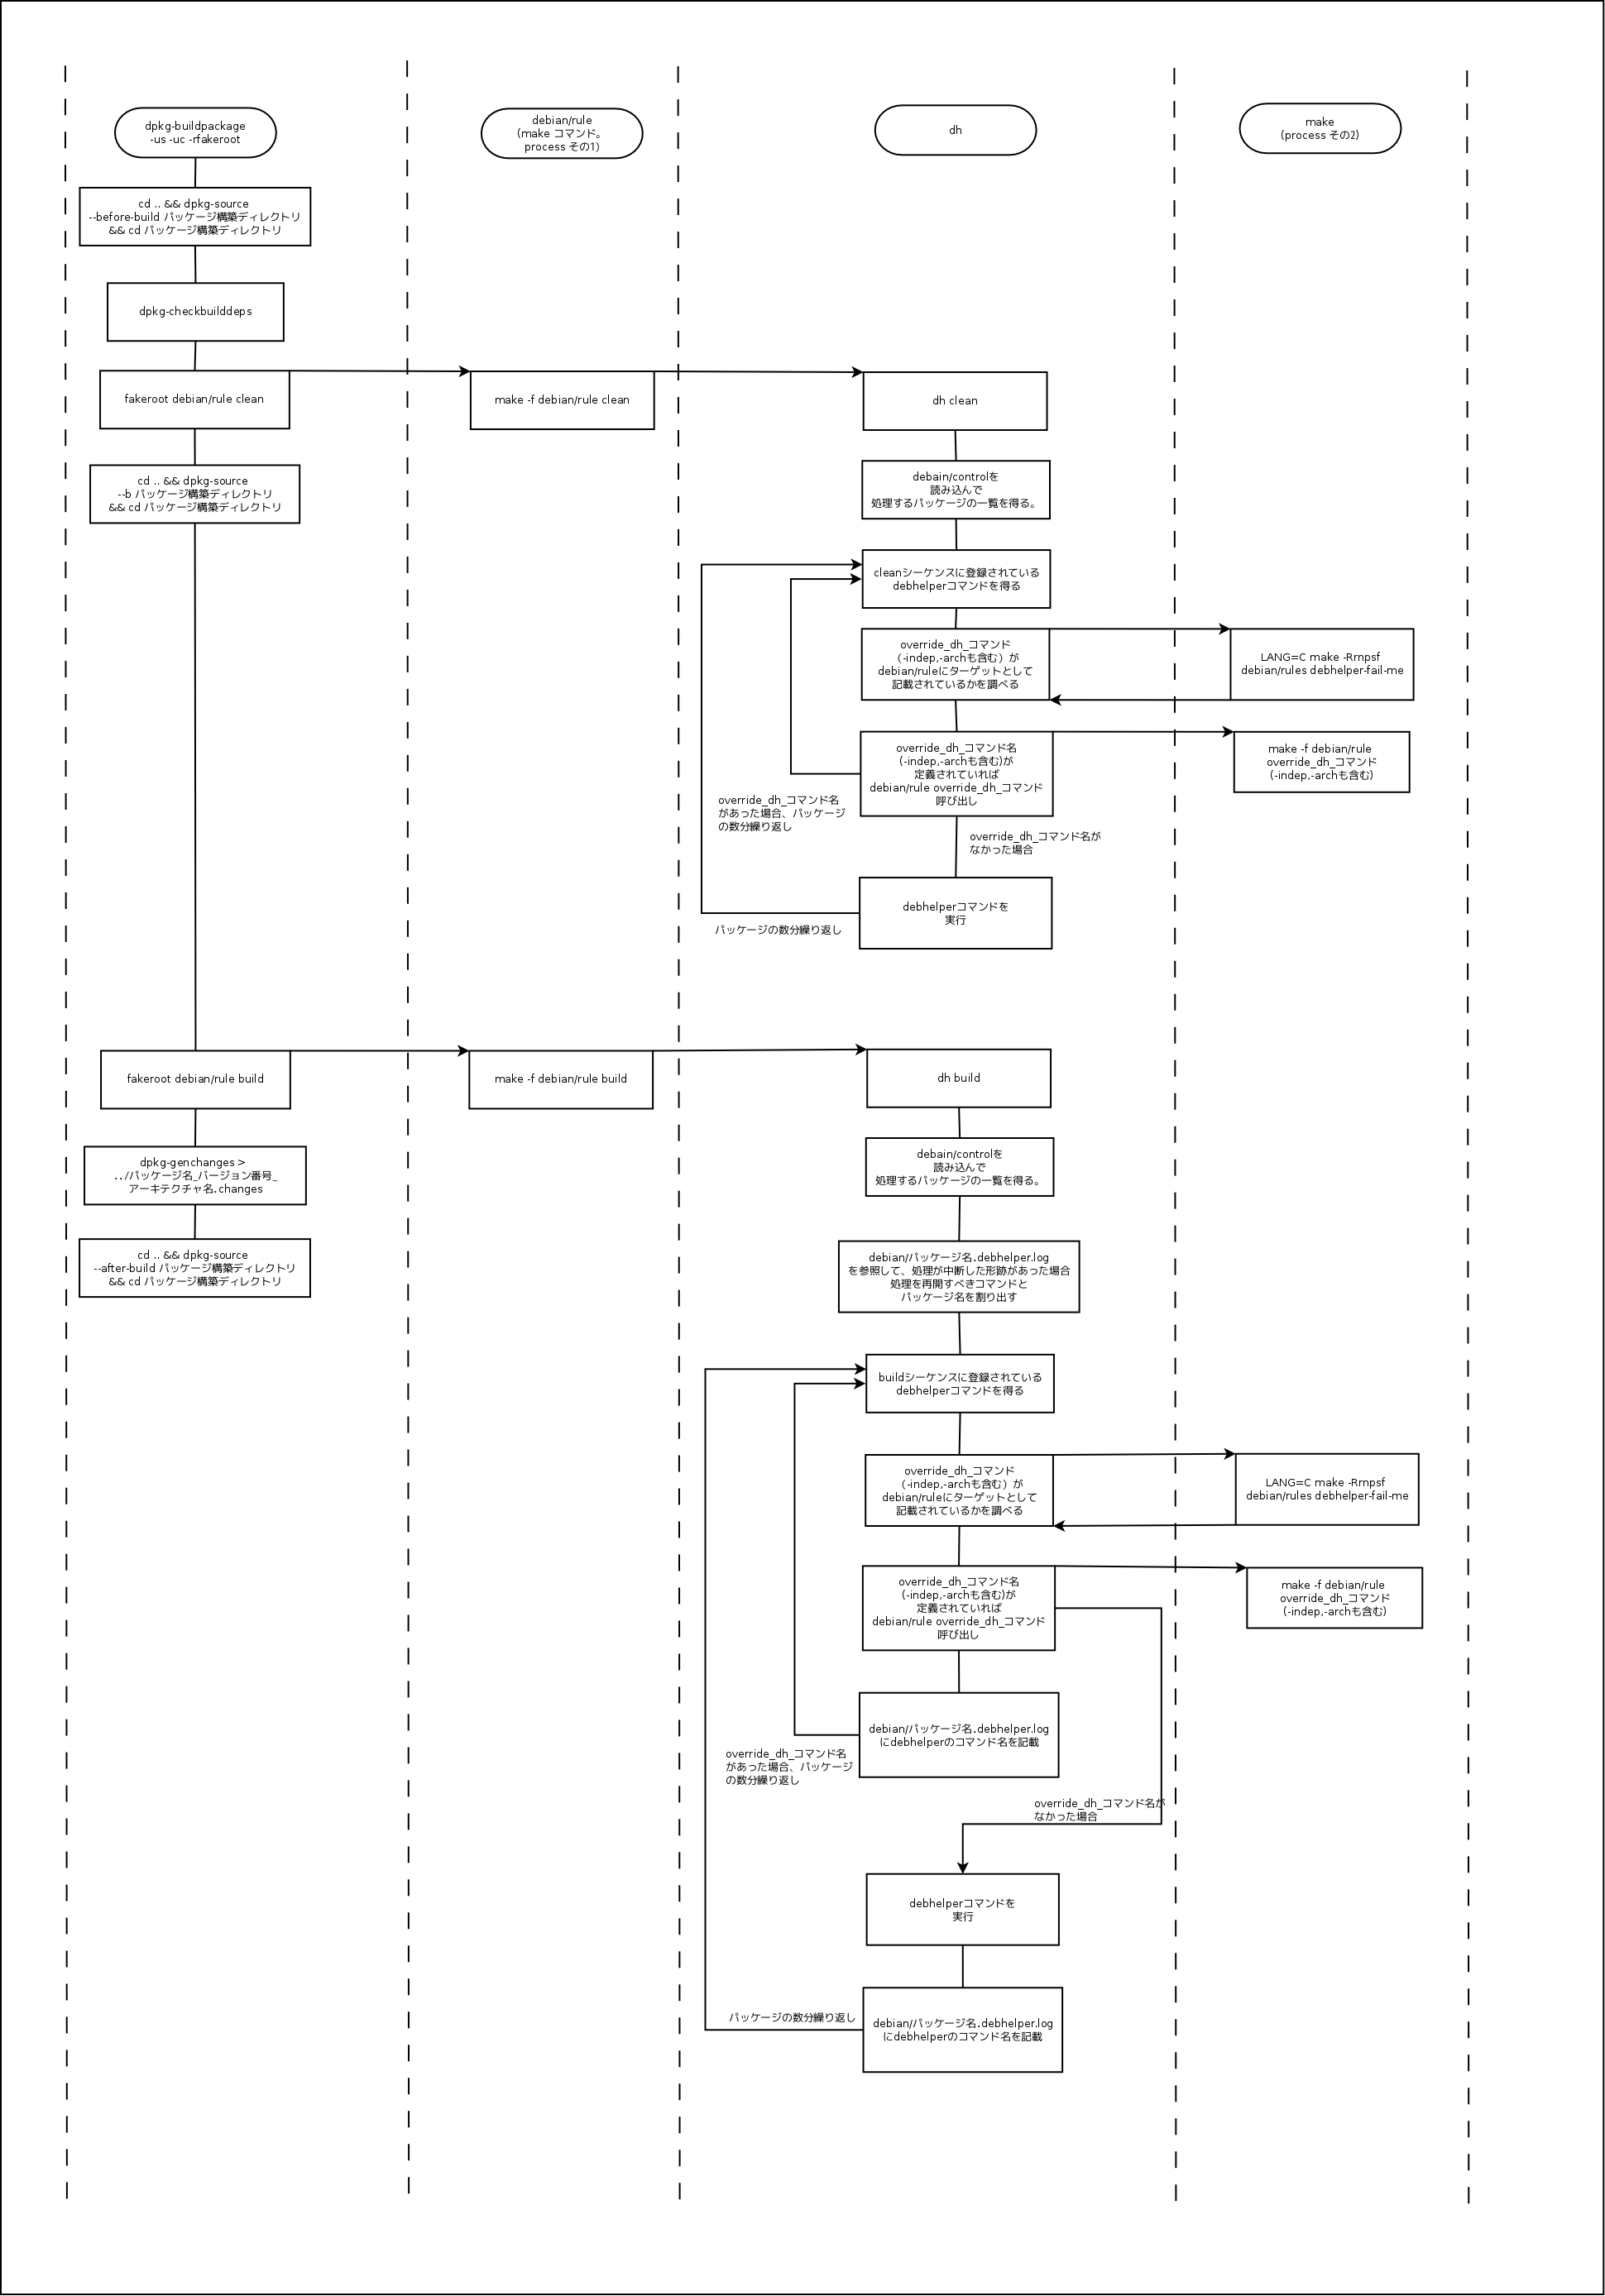
\includegraphics[width=17cm]{image201112/dh-internal-schema1.png}
  \end{center}
  \caption{dh内部動作}
  \label{fig:dh-internal-schema1}
\end{figure}

図\ref{fig:dh-internal-schema1}から判るように、dpkg-buildpackageから
makeコマンドが起動され、次にdhが起動され、
さらにdhからmakeが起動されるという関係になっている事が判ります。また、
override\_{\em debhelperコマンド名}ターゲットの処理を行うのに、makeコマンドを使って
処理をしているという事も判ります。

dhを使うと、makeコマンドはoverride\_{\em debhelperコマンド名}ターゲットの処理をする役目だけを
担当します。
そのうち、dhコマンドが進化すると、makeコマンドの力を借りなくてもパッケージ作成ができるようになる
かもしれませんね。

\subsubsection{``debian/パッケージ名.debhelper.log''ファイルについて}

最近のdhコマンドを使うdebian/rulesには、ファイルの依存関係についての記載がありません。この為、パッケージビルド中で処理が中断した場合、どこから再開すれば良いかをdebian/rulesでmakeが判定する事はできません。

実は、dhコマンドはclean以外のシーケンスが指定されると、''debian/パッケージ名.debhelper.log''というファイルに処理を行ったdebhelperコマンドを記録しています。ここで、万一dhの処理が中断した場合、処理をどこから始めれば良いかについてはこのログファイルを参照して処理の再開を行います。

``debian/パッケージ名.debhelper.log''の中身は以下のようになっています。

\begin{commandline}
debian/パッケージ名.debhelper.logの中身:
dh_auto_test
dh_prep
dh_installdirs
...中略...
dh_buiddeb
\end{commandline}

また、このファイルはdh cleanによって消去されます。なお、dh cleanの時には、このログファイルは作成されません。つまり、dh cleanの処理を中断した場合は、dh cleanは呼び出される一連のdebhelperコマンドは最初から実行されてしまいます。

なお、処理再開の場所は、このログファイルのみ参照して決める為、処理を中断した後に、パッケージのソースファイルを変更して再開させるような使い方はできません。例えば、ソースファイル中のあるファイルを変更した為、特定のパッケージのシーケンスについては再会時に全部やり直しが必要だったとしても、これを自動で検知することはできません。

\subsubsection{dpkg-buildflagとの関係}

dhは互換性度合い(COMPATABLITY LEVEL)のv9から、
パッケージ構築の時に使う環境変数を設定するため、内部でdpkg-buildflag相当の処理を
呼び出します。

その為、9をdebian/compatに指定すると、debhelperコマンドに設定される環境変数は、
\begin{enumerate}
\item /etc/dpkg/buildflags.confの中身
\item XDG\_CONFIG\_HOME/dpkg/buildflags.conf (XDG\_CONFIG\_HOMEは環境変数です)の中身
\item HOME/.config/dpkg/buildflags.conf (HOMEは環境変数です)の中身
\item DEB\_flag\_MAINT\_SET, DEB\_flag\_MAINT\_STRIP, DEB\_flag\_MAINT\_APPEND, DEB\_flag\_MAINT\_PREPEND, DEB\_BUILD\_MAINT\_OPTINS(全部環境変数です)の値
\end{enumerate}
により様々に変化します。どのように変わるかはman dpkg-buildflagを参照してください。

\subsection{今月のコマンドその2:dh\_testroot}

\subsubsection{dh\_testroot動作詳細}

 現在の実行ユーザがrootであるかどうかを確認するコマンドです。rootユーザでは無い場合、
エラーメッセージを出力して処理を中断します。

\subsubsection{dh\_testrootコマンドラインオプション}

 コマンドラインオプションは特にありません。何か指定しても無視されます。

\subsubsection{dh\_testrootを実行してみる}

早速、実行してみましょう。

\begin{commandline}
$ sudo dh_testroot
$ echo $?
0
$ dh_testroot
You must run this as root (or use fakeroot).
$ echo $?
255
$ fakeroot dh_testroot
$ echo $?
0
\end{commandline}
% $

このようにroot権限で実行するか、fakeroot経由で実行した時のみ0を返却します。

\subsubsection{次回の発表について}

次の発表者は勉強会で発表します。選ばれた人はよろしくおねがいします。

\clearpage

%------------------------------------------------------------------------------
\dancersection{月刊debhelper 第3回}{山田 泰資}
%------------------------------------------------------------------------------
\index{げっかんでぶへるぱー@月刊debhelper}
\index{debhelper}

\subsection{はじめに}
パッケージビルド手順を記述するdebian/rulesファイル。これを
簡潔化するためにdebhelperコマンド群(dh\_*)がありますが、
その一方で裏側で一体何がなされているのか掴み難くなって
しまいました。

本企画ではこのコマンド群を、毎月持ち回りで解説します。毎月2つ以上の
コマンドを解説し、次回発表の立候補が無い場合は発表者が次の発表者を
指名できるというルールで進めて行きます。

\subsection{今月のコマンド:dh\&dh\_auto\_* - シーケンスとビルドシステム}

dhコマンドの全体像については前回の野島さんの発表で既に解説されて
いるのですが、そこで「試しに読んでみるとよいと思います」とあったので、
実際に読みつついじってみました。その中でもう少し判ったことがあったので
報告します。

\subsubsection{dhの動作、再まとめ}
\index{dh}

dhコマンドを実行すると、デフォルトでは以下のコマンド群が
各シーケンス毎に呼ばれます:

\begin{table}[ht]
\begin{center}
\small
\begin{tabular}{|p{8em}|p{35em}|}
\hline
シーケンス名&シーケンスで実行されるコマンド \\
\hline
clean & dh\_testdir dh\_auto\_clean dh\_clean \\
build & dh\_testdir + (rules build-arch build-indep) \\
build-indep & dh\_testdir dh\_auto\_configure dh\_auto\_build dh\_auto\_test \\
build-arch & dh\_testdir dh\_auto\_configure dh\_auto\_build dh\_auto\_test \\
install &
\begin{minipage}[t]{\columnwidth}%
(rules build install-arch install-indep) + \newline
dh\_testroot dh\_prep dh\_installdirs dh\_auto\_install
dh\_install dh\_install*\newline
dh\_bugfiles dh\_ucf dh\_lintian dh\_gconf dh\_icons
dh\_perl dh\_usrlocal dh\_link\newline
dh\_compress dh\_fixperms
\end{minipage} \\
install-indep & (rules install-indep) + <上のinstallと同じ> \\
install-arch & (rules install-arch) + <上のinstallと同じ> \\
binary & (rules install binary-arch binary-indep) \\
binary-indep &
\begin{minipage}[t]{\columnwidth}%
(rules install-indep) +
dh\_installdeb dh\_gencontrol dh\_md5sums dh\_builddeb \\
\end{minipage} \\
binary-arch &
\begin{minipage}[t]{\columnwidth}%
(rules install-arch) + \newline
dh\_strip dh\_makeshlibs dh\_shlibdeps + <上のbinary-indepと同じ> \\
\end{minipage} \\
\hline
\end{tabular}
\caption{dhの各シーケンスで実行されるコマンド}
\label{tab:sequence-dh-commands}
\end{center}
\end{table}
かつてはrules(Makefile)に羅列されていたコマンド群が、
今はdhの中にPerlのリスト変数で管理されている形になります。
そしてdebhelperモジュール(*.pm)がロード時にリストの内容を
いじって実行内容を変更することでビルド過程をカスタマイズします。

わざわざmakeを使わず自前なのは、実行内容を変更するという
モジュール機構とoverride機構がmakeベースでは依存関係ツリーの
変更になり実現困難だったからでしょうか。たしかに拡張makeでも
使わない限り難しそうです(拡張makeまで行きたくないから現状の
実現方法・・・なんでしょうか)。

さて、今回の話題は、このモジュール機構になります。
普段何気なくどんなパッケージでもパッケージビルドされている訳ですが、
言語環境や開発者の選択によってビルド方法は千差万別です。これは
どうやって吸収されているのでしょうか?

\subsubsection{2つのモジュール:シーケンスとビルドシステム}
ここで登場するのが「シーケンス」とは別の、「ビルドシステム」
モジュールになります。この2つは
\begin{itemize}
\item シーケンスモジュールは(主に)前処理・後処理を追加し、適切なパッケージビルドが行われるようにする
\item ビルドシステムモジュールは各ソースパッケージに内包されるビルド方式を自動認識し、それを駆動する
\end{itemize}
と異なる役割を持ちます。典型的なconfigure\&makeパターンで説明すると、
\begin{enumerate}
\item Sequence/autotools\_dev.pm が config.sub/config.guess を最新に更新
\item Buildsystem/autoconf.pm が ./configure を発見・実行
\item Buildsystem/makefile.pm が Makefile を認識し、make でビルドやインストール
\end{enumerate}
といった連携リレーになります(autotools\_devは--withで有効化された場合のみ)。

\subsubsection{ビルドシステムの選択と連携}
さて、ビルドシステムは以下のフローで自動選択されています:
\begin{enumerate}
\item まず、Buildsystem/*.pmは全部ロードする
\item 各モジュールのcheck\_auto\_buildable APIにて「ビルドできる度」を照会
\item 同じクラス階層の中で一番大きい「ビルドできる度」を返したものを選択
\end{enumerate}
ポイントは
\begin{itemize}
\item この自動選択はconfigure/build/test/install/cleanの各段で毎回行われる
\item 同じクラス階層縛りがある
\end{itemize}
の2点です。つまり、
\begin{itemize}
\item 毎回行われるので、各段で応答・不応答を変えてモジュール間連携を行う
\item 自分が優先されるべき場合、親クラスの結果を上回るようにして勝つ
\end{itemize}
とする必要があり、「単純にビルドできるから真値を返す」という実装では
ないのでした。これは自前のビルドシステム拡張、特に他と連携する場合に
必要な留意事項になります。具体的にどういうコードなのかというとcmakeの
ものが参考になります:
\begin{commandline}
=== Buildsystem/cmake.pm ===
sub check_auto_buildable {
    my $this=shift;
    my ($step)=@_;
    if (-e $this->get_sourcepath(``CMakeLists.txt'')) {
        my $ret = ($step eq ``configure'' && 1) ||
                  $this->SUPER::check_auto_buildable(@_);
        # Existence of CMakeCache.txt indicates cmake has already
        # been used by a prior build step, so should be used
        # instead of the parent makefile class.
        $ret++ if ($ret && -e $this->get_buildpath(``CMakeCache.txt''));
        return $ret;
    }
    return 0;
}
\end{commandline}
%$
Makefileジェネレータとしてconfigureステージだけ担当のような
顔をしつつ、ビルドキャッシュがある場合は自分が後段も担当すべきとして
親であるmakefile.pmを押しのけて勝つ、というわけです。

\subsubsection{ビルドシステムは誰が呼んでいるのか}
ところでこのビルドシステム、誰が呼んでいるのでしょうか?例えばdhでは
\begin{commandline}
$ dh --buildsystem=perl_makemaker
\end{commandline}
%$
のように指定できるのですが、dhにはどこにもビルドシステムに関する
処理は書かれていません。

これはdhからオプションをそのままスルーパスされる形で
\footnote{Debianは、ビルドコマンド調査の時も思いましたが
コマンドライン引数の引き回し本当に多用しますね・・・}
dh\_auto\_(build\textbar{}clean\textbar{}configure\textbar{}install\textbar{}test)の
dh\_auto\_*系コマンド(だけ)が呼び出し元になっています。シーケンス中の
すべてのdh\_*コマンドに同様にスルーパスは届くのですが、反応するのが
この5つだけ、という訳です(man debhelperのBUILD SYSTEM OPTIONS)。
だからこそ独自処理を書く場合はrulesに
\begin{commandline}
override_dh_auto_build:
        ...
\end{commandline}
などとoverride\_dh\_auto\_*ターゲットを書くという話になるわけです。
dh\_auto\_*さえ止めれば、いかなるシーケンスが走ってもビルドシステム
呼び出しが行われず、実際のビルドは行われないからです。

これらのdh\_auto\_*コマンドは上のロード→照会(check\_auto\_buildable)\\
→API(configure\textbar{}build\textbar{}test\textbar{}install\textbar{}clean)
コールのトリガを引いているだけです。このフローの詳細はライブラリ化
されているので各コマンドは3行くらいしかありません。

\subsubsection{ビルドシステムの追加方法}
ビルドシステムの拡張は簡単で、以下のAPIを実装した*.pmをBuildsystem/
フォルダに置くだけです。基底クラスに空実装があるので全部書く必要はなく、
実際に処理を追加したいAPIのみ実装すれば十分です。
\begin{quote}
\begin{verbatim}
check_auto_buildable($step)                          # 必須
pre_building_step($step)                             # オプション
configure() build() test() install($destdir) clean() # いずれかを実装
post_building_step($step)                            # オプション
\end{verbatim}
\end{quote}
各APIの処理は名称から想像される通りで、先に解説済みのc\_a\_b API以外は
返値もありません(使われていません)。

サンプルとして、今は懐かしきimake/xmkmfを使ったソースパッケージの
自動検知+ビルドに対応するようにimake.pmモジュールを用意してみました:
\begin{commandline}
package Debian::Debhelper::Buildsystem::imake;
use strict;
use base 'Debian::Debhelper::Buildsystem::makefile';

sub DESCRIPTION { "imake (IMakefile)" }
sub new { shift->SUPER::new(@_); }
sub check_auto_buildable {
    my($self, $step) = @_;
    return 1 if ($step eq "configure" &&
                 glob($self->get_sourcepath("I[Mm]akefile")));
    return 0;
}
sub configure { shift->doit_in_sourcedir("xmkmf", "-a", @_); }
1;
\end{commandline}
こんな簡単なものでも、ktermなどの対象パッケージをビルドするには十分です。

なお、これを組み込むにはDh\_Buildsystems.pmのソース中の自動判定リストの
末尾に
\begin{commandline}
our @BUILDSYSTEMS = (``autoconf'', ..., ``imake'');
\end{commandline}
のようにモジュール名を追加してやる必要があります。

\subsubsection{まとめ}
本解説ではdhフレームワークを支えるビルドシステム部分を解説しました。
これはdh\_*コマンドとしてはdh\_auto\_*の5コマンドに対応し、これらを
通してビルドシステムが駆動されています。

\subsection{今月のコマンド:dh\_builddeb}
\index{dh\_builddeb}

dh\_builddebは、dhによって起動される一連のコマンドシーケンスの最後を
飾るコマンドです(ちなみに最初はdh\_testdir)。

マニュアルは「dpkg-deb を呼ぶだけのかんたんなおしごと\footnote{
dh\_builddeb simply calls dpkg-deb(1) to build a Debian package or packages.
}」と一行だけの解説ですが、これが意外にも中で色々としていてdh\_*コマンドの
勉強になります。

\subsubsection{何をしているの?}

やっていること自体は以下の3つです:
\begin{enumerate}
\item debhelper(7)のファイル排除指定があれば、その除去処理をする
\item deb/udeb形式の判定を行い、dpkg-debの起動分けをする
\item さらに、DEB\_BUILD\_OPTIONSのparallel=指定があれば、dpkg-debを並列駆動する
\end{enumerate}
マニュアルの解説が1行の割には、意外に仕事をしています。

\subsubsection{疑問:udebって何?}
\index{udeb}
実はudebの存在を知りませんでしたが、udebというのはDebian Installer(d-i)で
使用される*.deb風のパッケージです。形式としてはudebもdebも同じで
普通にdpkgで操作できるのですが、極小リソースでの限定的な利用を
想定しているためドキュメントはおろかチェックサム機能などまで外されています。
\begin{commandline}
=== debian/control ===
Section: debian-installer
...
XC-Package-Type: udeb
XB-Installer-Menu-Item: 1200 <- d-i menuでの表示制御パラメータ
\end{commandline}
のように特殊なヘッダが入っているcontrolがある場合、dh\_builddebは
自動的にudebビルドモードでdpkg-debを起動します。

他にもこういう特殊ヘッダはあるのだろうかとか、これを入れると
具体的に何をどう変えられるのかなどudebとd-iの話は更に掘ると
面白そうですが、今回は脱線ということでここまでにしておきます
\footnote{
資料としては http://d-i.alioth.debian.org/doc/talks/debconf6/paper/ かな?
}。
udeb固有処理は他のdh\_*コマンドにも多数含まれており、is\_udeb()で
様々な処理分けを裏側でしています。

\subsubsection{debhelper(7)系コマンドの実装パターン}
dh\_builddebの中を覗くと、各所で\$dh{...}という変数へのアクセスが
頻出しています。これはdh\_*コマンドのdebhelper(7)オプションの
パースや共通的な処理が Debian::Debhelper::Dh\_Lib ライブラリで
行われており、このライブラリとコマンド側の連携に \%dh という
グローバル変数が使われているためです。また \%ENV も多用されています。

コードの流れとしては、debhelperの純正(Perl製)dh\_*コマンドは
概ね以下の実装パターンになっています:

\begin{commandline}
use Debian::Debhelper::Dh_Lib; # init()関数などがインポートされる
init(options => { ``myopt=s'' => \&dh{MYOPT}, ... }); # @ARGVや%ENVの定型処理

# 含まれているパッケージの数だけ処理を反復
foreach my $package (@{$dh{DOPACKAGES}}) {
    # 上のinit()で取り込まれた結果を見ながら処理をする
    if ( $dh{...}) { ... # Dh_Lib.pm の API を呼んだりするなど ... }
    # 自動的に取り込まれない環境変数(コマンド固有)は自分で処理する
    if ($ENV{...}) { ... # 上記同様 ... }
}
\end{commandline}

dh\_builddebの場合は、上のループの中が不要ファイルの削除と
dpkg-debの起動になり、これが例えばdh\_stripの場合は各生成中パッケージの
ワーキングフォルダをスキャンして、しかるべきファイルをstripして回ると
いうようになります。

\subsubsection{まとめ}
dh\_builddebコマンドの解説と、そこから出てきた疑問と共通的な構成の解説を
行ってみました。dh\_*コマンドは実質1行しかないものから1000行に迫るものまで
色々ありますが、dh\_builddebはちょうど理解する上で手頃な大きさです。

\clearpage

%-------------------------------------------------------------------------------
\dancersection{月刊debhelper 第4回}{山本 浩之}
%-------------------------------------------------------------------------------
\index{げっかんでぶへるぱー@月刊debhelper}
\index{debhelper}

\subsection{パッケージのmakeの前に…}

先月までに学んできたように、debhelper は、基本的にビルドに必要な一連のdh\_XXX コマンドを自動実行します。

例えばdebhelperは、dh\_auto\_configureというコマンドを提供しており、これはご想像の通り、
\begin{commandline}
./configure --build='dpkg_architecture_value("DEB_BUILD_GNU_TYPE")' --prefix=/usr --includedir=/usr/include \
--mandir=/usr/share/man --infodir=/usr/share/info --sysconfdir=/etc --localstatedir=/var \
--libdir=/usr/lib/\$multiarch --libexecdir=/usr/lib/\$multiarch --disable-maintainer-mode \
--disable-dependency-tracking --host='dpkg_architecture_value("DEB_HOST_GNU_TYPE")
\end{commandline}
をしているだけです。

しかし、メンテナによってautotoolsを利用し、confugureスクリプトをビルドの度に毎回configure.acから生成したい人もいるでしょうし、もしかするとMakefileの元となるMakefile.inだって、毎回Makefile.amから生成したい人もいるでしょう。
また、Debianパッケージオリジナルのパッチをあててパッケージを作るのは、ごく当たり前のように行なわれています。

そこで今月は、一連のdh\_XXXXコマンドへの追加の仕組みと、その例として、dpatchパッケージで提供されるdh\_dpatch\_patchコマンドと、autotools-devパッケージで提供されるdh\_autotools-dev\_updateconfigコマンドの追加について解説しましょう。

\subsection{一連のdh\_XXXXコマンドへの追加の仕組み}

基本となる一連のdh\_XXXXコマンドは、大元のコマンドであるdhスクリプトに記述してあり、すべてについては先月や先々月に話されているので、割愛します。

特にmake直前に実行されるものは、
\begin{commandline}
dh_testdir  #カレントディレクトリの確認
dh_auto_configure  #./configureの実行
\end{commandline}
だけです。

勿論、これだけではパッチもあてられないですし、configureスクリプトの再生成もできません。

そこでdhスクリプトは、一連のdh\_XXXコマンドを列挙する配列にし、これを\$sequences{\$sequence}のスカラ変数として保持しています。(この辺はperlにあまり詳しくないので、ちょっと間違っているかも…)

また、この\$sequencesからdh\_XXXXコマンドを除いたり(remove\_command)、あるdh\_XXXXコマンドの前に追加する(insert\_before)サブルーチンも用意されています。

dhスクリプトは、/usr/share/perl5/Debian/Debhelper/Sequence/ディレクトリのなかにあるファイルを参照しており、ここに
\begin{commandline}
insert_before("dh_auto_configure", "dh_new_command")
\end{commandline}
という記述のあるファイル(アドオン)が追加されると、dh\_auto\_configureの前にdh\_new\_command が実行されるようになります。

ただし、rulesの
\begin{commandline}
dh $@ --with 〜
\end{commandline}
%$
でアドオンが指定されない限り評価はされないので、ビルドに不必要なdh\_XXXXコマンドを入れていても大丈夫なはずです。

\subsection{dh\_dpatch\_patchコマンド}

dpatchパッケージをインストールすると、/usr/share/perl5/Debian/Debhelper/Sequence/ディレクトリにdpatch.pmファイルが入り、これには、
\begin{commandline}
insert_before("dh_auto_configure", "dh_dpatch_patch")
insert_before("dh_clean", "dh_dpatch_unpatch")
\end{commandline}

という記述があります。これは見て想像できるとおり、makeの直前に実行される./configureのさらに直前に、dh\_dpatch\_patchを加えています。
また、下の記述は、以前にビルドしたことがある場合に、パッチする前の状態にするdh\_dpatch\_unpatchコマンドも追加されています。

このdh\_dpatch\_patchは、パッケージソースのdebian/patches/00listに記述されたファイル名のパッチを先頭からパッチするコマンド、dpatchスクリプトを実行します。

すなわち、もしconfigureスクリプトにdpatchでなんらかのパッチをあてて実行したければ、dpatchパッケージをBuild-depし、debian/patches/ディレクトリにパッチファイルとそれに合わせた00listファイルを用意し、
\begin{commandline}
dh $@ --with dpatch
\end{commandline}
とrulesファイルに記述しておけば良いはずです。

makeだけしたいならば、ターミナルで、
\begin{commandline}
$ dh_dpatch_patch
$ ./configure 〜
$ make
\end{commandline}
%$
でも大丈夫です。

\subsection{autotoolsだって使いたい}

ビルドするマシンの環境に合わせて、configureスクリプトなどを調整してくれるツールとして、GNU autotoolsというものがあります。次にこのGNU autotoolsをdebhelperで利用する方法について述べましょう。

\index{dh-autoreconf}
dh-autoreconfパッケージをインストールすると、依存関係でautomake、autoconfと、automakeに依存してautotools-devがインストールされます。
autotools-devパッケージは\\
/usr/share/perl5/Debian/Debhelper/Sequence/ディレクトリにautotools-dev.pmファイルが入ります。
これには、
\begin{commandline}
insert_before("dh_auto_configure", "dh_autotool-dev_updateconfig")
insert_before("dh_clean", "dh_autotool-dev_restoreconfig")
\end{commandline}
と記述されています。

dh\_autotool-dev\_updateconfigコマンドは、カレントディレクトリ以下で実行しているシステムタイプの標準名を推測するためのconfig.guessとconfig.subファイルを探し、config.guess.dh-origとconfig.sub.dh-origファイルに名前を換え、それぞれ/usr/share/misc/ディレクトリにある最新autotool-devのconfig.guessとconfig.subをコピーしてきます。

dh-autoreconfパッケージは/usr/share/perl5/Debian/Debhelper/Sequence/ディレクトリにautoreconf.pmファイルが入ります。
これには、
\begin{commandline}
insert_before("dh_auto_configure", "dh_autoreconf")
insert_before("dh_clean", "dh_autoreconf_clean")
\end{commandline}
と記述されています。

dh\_autoreconfコマンドは、簡単に言うと、automake、autoconfをしてくれるautoreconfスクリプトを呼び出し、configureやMakefile.inを再生成します。

dh\_autoreconfを使いたいときは、このパッケージにBuild-depし、
\begin{commandline}
dh $@ --with autoreconf
\end{commandline}
%$
とrulesファイルに記述しておけば良いはずです。
debian/autoreconfファイルにディレクトリのリストがあれば、そこだけconfigureやMakefile.inを更新してくれます。

autoreconf.pmファイルでは「dh\_auto\_configureより前だよ」という指定しかありませんから、dh\_autoreconfが実行されてパッチがあてられるのか、パッチがあてられてからdh\_autoreconfが実行されるのかまでは記述されていません。
dhスクリプトを見た限りでは「--with」オプションの順でリストされているようです。つまり、dh-autoreconfパッケージを利用するソースパッケージのMakefileに対してBTSでパッチを書く場合は、「--with」オプションの順を確認する必要がありそうです。

\subsection{おわりに}

今回はmakeを実行する前に使用されるconfigureスクリプトなどの、debhelperを使ったカスタマイズ法について、駆け足で説明してみました。

\clearpage

%-------------------------------------------------------------------------------
\dancersection{月刊debhelper 第5回}{杉本 典充}
%-------------------------------------------------------------------------------
\index{げっかんでぶへるぱー@月刊debhelper}
\index{debhelper}


\subsection{今月のコマンド:dh\_md5sums}
\index{dh\_md5sums}

dh\_md5sumsコマンドは「DEBIAN/md5sumsファイルを生成する」コマンドです。

\subsubsection{DEBIAN/md5sumsファイルについて}
「\$ ar x debian-package.deb」を実行し現れるcontrol.tar.xxファイルを展開
するとmd5sumsファイルが出てきます。このmd5sumsファイルはdata.tar.xxファイルに含むファイルそれぞれから取得したmd5sumを記述しています。

\begin{commandline}
$ apt-get download hello-debhelper
$ ar x hello-debhelper_2.7-3_i386.deb
$ ls
control.tar.gz  data.tar.gz  debian-binary  hello-debhelper_2.7-3_i386.deb
$ tar xf control.tar.gz
$ ls
control         data.tar.gz    hello-debhelper_2.7-3_i386.deb
control.tar.gz  debian-binary  md5sums
$ head -n 1 md5sums
098518cc321f0467dc0e7c67f65e2cc1  usr/bin/hello
\end{commandline}
%$

\subsubsection{パッケージのビルド処理におけるdh\_md5sumsの実行}
dh\_md5sumsコマンドはインストールするファイルのmd5sumを取得する処理のため、ビルド処理の終盤で実行されます。

\begin{commandline}
$ apt-get source hello-debhelper
$ cd hello-debhelper-2.7
$ debuild -uc -us
  (省略)
  dh\_gencontrol -a
  dh\_md5sums -a
  dh\_builddeb -a
  (省略)
$ ls debian/hello-debhelper
DEBIAN   usr
$ head -n 1 debian/hello-debhelper/DEBIAN/md5sums
098518cc321f0467dc0e7c67f65e2cc1  usr/bin/hello
\end{commandline}
%$

\subsubsection{コマンドのオプション}

\begin{table}[ht]
\caption{dh\_md5sumsのコマンドラインオプション一覧}
\begin{center}
\small
\begin{tabular}{|p{12em}|p{33em}|}

\hline
オプション&説明 \\
\hline
-x,  --include-conffiles & DEBIAN/conffilesファイルに記述した設定ファイルのmd5も生成します。\\
\hline
-Xitem, --exclude=item & md5sumの生成を除外するファイル名を指定します。ただしディレクトリが別でもファイル名が一致すればどちらも除外されます。 \\
\end{tabular}
\end{center}
\end{table}

\subsection{今月のコマンド:dh\_strip}
\index{dh\_strip}

dh\_stripコマンドは「実行ファイル、共有ライブラリ、スタティックライブラリをstripする」コマンドです。

\subsubsection{デバッグシンボルの扱い方を制御する}
オプションなしや環境変数を指定せずにdh\_stripコマンドを実行するとコンパイルしたオブジェクトファイルのデバッグシンボルをstripするのが通常の処理です。しかし、デバッグを目的とする場合はデバッグシンボルをstripしてしまうとデバッガが十分に機能しないため困ります。

dh\_stripコマンドではデバッグシンボルを以下のように扱うことができます。\cite{debugpackage}

\begin{itemize}
 \item オプションなしで実行すると、stripする。
 \item 環境変数DEB\_BUILD\_OPTIONS=nostripを指定して実行すると、stripしない。(処理的にはdh\_stripが即座に終了する)
 \item --dbg-packageオプションを指定すると、/usr/lib/debug配下にデバッグシンボルを分離して残すパッケージ(=デバッグパッケージ)を作成する。
\end{itemize}

\subsubsection{デバッグパッケージを作成するための条件}
debhelperの機能を利用するとstrip済みのバイナリパッケージに加えて簡単にデバッグパッケージを作成できます。デバッグパッケージを追加で作成したい場合は以下の処理を記述してパッケージをビルドすればよいです。

\begin{itemize}
 \item CFLAGSなどのコンパイルオプションに''-g'を付与しビルド時にデバッグシンボルを生成するようにする。
 \item debian/rulesでoverride\_dh\_stripを定義し、dh\_strip --dbg-package=package-dbgを処理させる。
 \item debian/controlにパッケージ「package-dbg」の定義を記述する。このとき、パッケージ「package-dbg」はパッケージ「package」にバージョン指定をしてdependすること。
\end{itemize}

\subsubsection{コマンドのオプション}

\begin{table}[ht]
\caption{dh\_stripのコマンドラインオプション一覧}
\begin{center}
\small
\begin{tabular}{|p{12em}|p{33em}|}
\hline
オプション&説明 \\
\hline
-Xitem, --exclude=item & 指定した文字列を含むファイルをstrip処理の対象から除外する。複数のファイルを指定したい場合はオプションを複数回指定することも可能。\\
\hline
--dbg-package=package & デバッグシンボルを含むパッケージ「package-dbg」を作成する。 \\
\hline
-k, --keep-debug & パッケージをビルドした作業ディレクトリ内のusr/lib/debugにstrip後のデバッグシンボルファイルを残す。--dbg-packageオプションの指定で事足りる場合は多いが、より細かくデバッグシンボルを扱いたい場合を想定して用意されている。 \\
\end{tabular}
\end{center}
\end{table}

\begin{thebibliography}{0}
\bibitem{debugpackage} Debian Wiki - DebugPackage \url{http://wiki.debian.org/DebugPackage}\
\bibitem{bestpkgpractice} Debian.org 第6章パッケージ化のベストプラクティス \url{http://www.debian.org/doc/manuals/developers-reference/best-pkging-practices.html}
\end{thebibliography}

\clearpage

%-------------------------------------------------------------------------------
\dancersection{Debian開発者のKDE環境あれこれ}{野島 貴英}
%-------------------------------------------------------------------------------
\index{DebianかいはつしゃのKDEかんきょう@Debian開発者のKDE環境}
\index{kde}

最近のDebianをそのままインストールすると、特に指定しない場合GNOMEという
デスクトップ環境がインストールされます。しかしながら、Debianではいくつも
デスクトップ環境が用意されており、ユーザは自由にこれらを選んで使うことが
できます。デスクトップ環境はユーザにとってはいつも使う環境ですから、
いろいろとこだわりもあるかとおもいます。今回はそんな中、KDEというデスクトップ環境に
ついてあれこれ語ってみます。

\subsection{利用者としてのKDE導入方法}

Debianの安定版の利用を検討していて、KDE環境をいわゆる利用者として
使う為にインストールするやり方について簡単に述べます。

\begin{enumerate}
 \item 安定版のDebianのインストールDVDを用意します。
 \item インストーラのメニュー画面が出ましたら、TABキーをおすと画面下の方に編集可能な行
が現れますので、以下の例ように ``desktop=kde''という文言を追加します。なお、日本語106キー
ボードを使っている場合、キートップの刻印の通りに ``='' を押しても ``=''文字が入力できない場合が
ありますが、この場合は ``\verb|^|'' の刻印のキーを押すと ``='' 文字が入力できます。

\begin{commandline}
 /install.amd/vmlinuz vga=788 initrd=/install.amd/initrd.gz --- quiet desktop=kde
\end{commandline}

\begin{figure}[ht]
\begin{center}
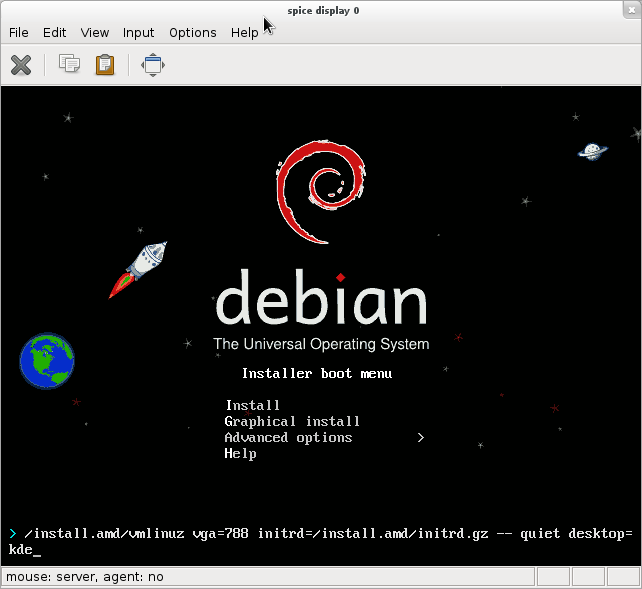
\includegraphics[width=7cm]{image201202/kdedesk/stable-inst-menu.png}
\caption{安定版インストール画面でTABキーを押したときの様子}
\end{center}
\end{figure}
\item あとは通常どおりインストールを行います。インストールを進めていくと
「インストールするソフトウェアの選択:」のメニューが現れますので、 ``Debian desktop environment''
を選択しておいてください。
\item インストールが完了しましたら、リブートを行います。
\item KDE環境が起動します。
\end{enumerate}

以上となります。簡単ですね。

\subsection{開発者としてのexperimental版KDE導入方法(KVM+spice)}
\label{sec:exp-kde}
\index{kvm}
\index{spice}

東京エリアDebian勉強会にいらっしゃるような方々には、前述のインストールと環境では
きっと「ぬるゲー(笑)」な感じのはずです。その場合、是非とも
experimental版のKDE環境を利用いただき、BTS書き/パッチ開発/翻訳/デバッグなどの
開発活動に勤しんでみましょう。ここでは、開発者向けKDE環境導入について簡単に述べます。

\begin{itemize}
\item 開発者向けにexperimental版導入を前提にします。
\item 仮想環境であるKVMを利用して仮想環境上に導入します。これなら、ディスクイメージファイルをとっておけば、
うっかりexperimental環境でaptitude full-upgradeして全く立ち上がらなくなっても(実話)あっさり復帰できます。
\item サウンドももちろん欲しいので仮想デスクトップ環境としてspiceを使います。
\item いつでもどこでも開発できるようにモバイル環境に構築します。
\end{itemize}
図\ref{fig:kde-env}のKDE開発環境の用意を想定します。

\begin{figure}[ht]
\begin{center}
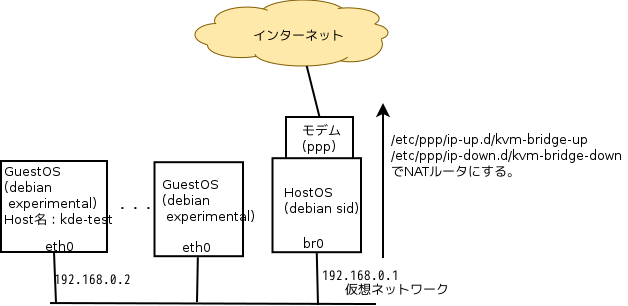
\includegraphics[width=10cm]{image201202/kdedesk/kde-dev-env.png}
\caption{\label{fig:kde-env}KDE開発環境}
\end{center}
\end{figure}

以下は導入に関しての流れです。(細かい事は割愛します。操作にあたっては適宜root権限が必要だったりします)
\begin{enumerate}
\item HostOSとなるPCのBIOSを操作して、CPUの仮想技術支援機構のスイッチをONにしてブートしておきます。
\item HostOSに\url{http://www.debian.org/CD/netinst}から名刺サイズのCDイメージを落として置きます。
\item HostOSの/etc/network/interfacesに以下の追記を行い、br0を作っておきます。
\begin{commandline}
# 追記はここから。aptitude install bridge-utilsはやっておくこと。
auto br0
iface br0 inet static
        address 192.168.0.1
        netmask 255.255.255.0
        bridge_ports none
        bridge_stp off
        bridge_fd 0
        bridge_maxwait 0
\end{commandline}
\item HostOSの/etc/sysctl.d/bridge-filter-workaround.confを作り、\\
sysctl -p /etc/sysctl.d/bridge-filter-workaround.confを実行して、br0のフィルタを無効化しておきます。
\begin{commandline}
# /etc/sysctl.d/bridge-filter-workaround.confの中身
net.bridge.bridge-nf-call-ip6tables = 0
net.bridge.bridge-nf-call-iptables = 0
net.bridge.bridge-nf-call-arptables = 0
\end{commandline}
\item HostOSの/etc/ppp/ip-up.d/kvm-bridge-up,/etc/ppp/ip-down.d/kvm-bridge-downを作っておきます。他にフィルタとか必要であれば適当にどうぞ。
\begin{commandline}
#!/bin/sh
# /etc/ppp/ip-up.d/kvm-bridge-upの中身
PATH=/bin:/usr/bin:/sbin:/usr/sbin
CDPATH=
sysctl -w net.ipv4.ip_forward=1
iptables -t nat -A POSTROUTING -o $PPP_IFACE -j MASQUERADE
iptables -A FORWARD -i br0 -o $PPP_IFACE -j ACCEPT
\end{commandline}
\begin{commandline}
#!/bin/sh
# /etc/ppp/ip-down.d/kvm-bridge-downの中身
#!/bin/sh
PATH=/bin:/usr/bin:/sbin:/usr/sbin
CDPATH=
sysctl -w net.ipv4.ip_forward=0
iptables -t nat -D POSTROUTING -o $PPP_IFACE -j MASQUERADE
iptables -D FORWARD -i br0 -o $PPP_IFACE -j ACCEPT
\end{commandline}
\item HostOSにkvm/libvirt/spice-client-gtkパッケージを導入しておきます。
\item HostOSにてGuestOS用のkde-test.xmlを以下の雛形で作成してvirsh define kde-test.xmlしておきます。\footnote{virt-installは何故か自分のexperimentalな環境ではSegmentation Faultで落ちてしまうのでここでは使いません。BTSしときます。}
\begin{commandline}
<domain type='kvm'>
  <name>kde-test</name>
  <memory>1048576</memory>
  <vcpu>1</vcpu>
  <os>
    <type arch='x86_64' machine='pc-1.0'>hvm</type>
    <boot dev='hd'/>
    <boot dev='cdrom'/>
    <bootmenu enable='yes'/>
  </os>
  <features>
    <acpi/>
    <apic/>
    <pae/>
  </features>
  <clock offset='utc'/>
  <on_poweroff>destroy</on_poweroff>
  <on_reboot>restart</on_reboot>
  <on_crash>restart</on_crash>
  <devices>
    <emulator>/usr/bin/kvm</emulator>
    <disk type='file' device='disk'>
      <driver name='qemu' type='raw' cache='writeback'/>
      <source file='/var/lib/libvirt/images/kde-test.img'/>
      <target dev='vda' bus='virtio'/>
    </disk>
    <disk type='file' device='cdrom'>
      <driver name='qemu' type='raw'/>
<!-- directory of cdimageは適当に変更ください -->
      <source file='/directory of cdimage/debian-6.0.4-amd64-businesscard.iso'/>
      <target dev='hdc' bus='ide'/>
      <readonly/>
    </disk>
    <controller type='ide' index='0'/>
    <interface type='bridge'>
<!-- macアドレスは適当に変更ください -->
      <mac address='52:54:00:31:cd:5a'/>
      <source bridge='br0'/>
      <model type='virtio'/>
    </interface>
    <serial type='pty'>
      <target port='0'/>
    </serial>
    <console type='pty'>
      <target type='serial' port='0'/>
    </console>
    <input type='mouse' bus='ps2'/>
    <graphics type='spice' port='5900' autoport='no'>
      <clipboard copypaste='yes'/>
    </graphics>
    <sound model='ac97'\>
    <video>
      <model type='qxl' vram='9216' heads='1'/>
    </video>
    <memballoon model='virtio'>
    </memballoon>
  </devices>
</domain>
\end{commandline}
\item HostOSで仮想環境用のディスクを10GBぐらいで作っておきます。
\begin{commandline}
qemu-img create -f raw /var/lib/libvirt/images/kde-test.img 10G
\end{commandline}
\item HostOSでKVMを起動して、spiceクライアントを接続します。
\begin{commandline}
virsh start kde-test; spicy -h 127.0.0.1 -p 5900 &
\end{commandline}
\item GuestOSのDebianインストーラが起動したら、TABキーを押し、画面下に現れた編集可能な行に、''priority=medium''を以下のように入力してインストールを開始します。
\begin{commandline}
 /install.amd/vmlinuz vga=788 initrd=/install.amd/initrd.gz --- quiet priority=medium
\end{commandline}
インストール途中「Debian アーカイブのミラーを選択」のメニューにて''sid''を選択し、「インストールするコンポーネント」として「sshサーバー」のみ(他は選択しない)とします。
\item インストールが完了すると、テキストコンソールからDebian sidなGuestOSへログインできるようになります。
\item GuestOSにログインして以下の行を/etc/apt/source.listへ付け加えます
\begin{commandline}
#追加内容
deb http://ftp.jp.debian.org/debian/ experimental main
deb-src http://ftp.jp.debian.org/debian/ experimental main
\end{commandline}
\item GuestOSの/etc/apt/preference.dにDebian KDEチーム製のexperimentalパッケージ用preferenceファイルをインストールします。
\begin{commandline}
cd /etc/apt/preference.d && wget http://pkg-kde.alioth.debian.org/files/kde-experimental
\end{commandline}
\item GuestOSで以下を実行し、experimentalなKDE環境を一気に入れてしまいます。
\begin{commandline}
aptitude update;aptitude aptitude install task-kde-desktop task-japanese-kde-desktop;aptitude clean
\end{commandline}
\item インストールが終わったら、GuestOSをリブートします。GuestOSでKDEのexperimental版が起動し、グラフィカルなログイン画面が現れます。
\end{enumerate}

\subsection{DebianとKDE環境のバージョン}

DebianのバージョンとKDEのバージョンの対応を表\ref{tab:kde-ver}に載せます。

\begin{table}[ht]
\begin{center}
\begin{tabular}{|l|l|l|l|l||l|}
\hline
Debian&stable&testing&unstable&experimental&upstream\\
\hline \hline
KDE &4.4&4.6&4.6&4.7.4&4.8.0\\
\hline
\end{tabular}
\caption{\label{tab:kde-ver}DebianのバージョンとKDEのバージョン}
\end{center}
\end{table}

KDEのupstreamは2012年1月25日に4.8.0をリリースしたばかりなので、まだ
experimentalも追いついていない状態です。

\subsection{KDE環境の開発の特徴}

KDE環境の開発は以下のような特徴があります。

\begin{enumerate}
\item Qt(キュート)ライブラリを使う。
\item C++のコードが基本
\item autotoolsの代わりにcmakeが使われる
\end{enumerate}

このため、Debianではパッケージ開発の為にpkg-kde-toolsパッケージが用意されています。

\subsection{DebianでのKDE環境のパッケージ開発}

DebianではKDE環境のパッケージ開発用にpkg-kde-toolsというパッケージを別に用意しています。こちらを導入するとKDE環境のパッケージ構築の際に便利な機能が使えるようになります。

\begin{table}[ht]
\begin{center}
\begin{tabular}{|l|l|l|l|}
\hline
項番&拡張されるもの&拡張&備考\\
\hline
1&dh& --with kde & debhelperにkde用の拡張を指定\\
\hline
2&dh\_auto\_*& --buildsystem=kde & dh\_auto\_*がcmakeを使うようになる、KDE環境用の設定を行う等\\
\hline
3&CDBS&kde.mk& CDBSでKDE用の拡張が利用できるようになる\\
\hline
4&その他&variables.mkなど& debian/rulesの中で\$(DEB\_CMAKE\_KDE4\_FLAGS)などが使える等\\
\hline
\end{tabular}
\caption{\label{tab:pkg-kde-tools-inst}pkg-kde-toolsをインストールした時の拡張}
\end{center}
\end{table}

\subsection{超簡易的にKDE用プログラムのDebianパッケージを作ってみる}

ここでは超簡易的にKDE用プログラムのDebianパッケージを作ってみます。
まず、事前準備として、

\begin{itemize}
\item 環境は\ref{sec:exp-kde}章のexperimental環境を用意ください。
\item  必要なパッケージ(cmakeパッケージ等)
\footnote{KDE環境向けの開発が全く初めての人は、細かい事が判ってくるまで、aptitude build-dep kdeutilsしておいてKDEパッケージ開発に必要なパッケージをあらかじめまとめて導入しておくという手もあります}
\end{itemize}

次にkhello-1.0.0/なるディレクトリに\url{http://techbase.kde.org/Development/Tutorials/First_program}にある、main.cppとCMakeLists.txtを配置します。

\begin{commandline}
$ cd khello-1.0.0
$ ls
CMakeLists.txt main.cpp
$
\end{commandline}
% $

次に、オリジナルのtar.gzアーカイブを作成しておきます。

\begin{commandline}
$ cd ..
$ tar czf khello_1.0.0.orig.tar.gz khello-1.0.0
$ ls -F
khello-1.0.0/  khello_1.0.0.orig.tar.gz
$
\end{commandline}

dh\_make を使ってdebian/ディレクトリを仕込みます。あとはrulesファイル以外
いつも通り、パッケージを作成するようにファイルを作成しておきます。

\begin{commandline}
$ cd khello-1.0.0/debian
$ ls -F
README.Debian  changelog  control    docs   source/
README.source  compat     copyright  rules
$
\end{commandline}
% $

pkg-kde-toolsパッケージを利用するrulesファイルを記載します。

\begin{commandline}
# pkg-kde-toolsを使ったKDE開発用debian/rulesファイルの中身。

%:
       dh $@ --with kde
\end{commandline}
%$

あとは、dpkg-buildpackage -uc -us -rfakerootを実行してビルドします。

\begin{commandline}
$ dpkg-buildpackage -us -uc -rfakeroot
dpkg-buildpackage: source package khello
...中略...
dpkg-source: info: building khello in khello_1.0.0-1.debian.tar.gz
dpkg-source: info: building khello in khello_1.0.0-1.dsc
 debian/rules build
dh build  --with kde
   dh_testdir
   dh_auto_configure --buildsystem=kde
-- The C compiler identification is GNU
-- The CXX compiler identification is GNU
...中略...
\end{commandline}
%$

無事、--buildsystem=kdeが利用され、cmakeが実行されています。

しばらく待つと無事にkhello\_1.0.0-1\_amd64.debなどが出来上がります。

ほら、pkg-kde-toolsのおかげでパッケージ開発も簡単でしょ?でしょ?

\subsection{おわりに}

今回は、Debian開発者の為のKDE環境の構築と、簡単なパッケージ作成について、
一通り記載してみました。これを機に、KDE環境に関する開発をされる方が増えると
うれしいと思っています。

\subsection{参考文献}

\begin{itemize}
\item \url{http://pkg-kde.alioth.debian.org/} Debian KDE Teamのホームページ。
\item \url{http://techbase.kde.org} KDE Techbase
\item \url{http://kde.org/} KDE本家
\item \url{http://www.spice-space.org/} SPICE仮想デスクトップデバイス本家
\end{itemize}

\clearpage
%-------------------------------------------------------------------------------
\dancersection{CMakeを使ってみる}{野島 貴英}
%-------------------------------------------------------------------------------
\index{cmake}

\subsection{CMakeとは}

KDE環境の開発に使われているツールにCMakeがあります。これは従来のautotools
のようなものです。が、autotoolsに比べて次に述べる代表的な特徴があります。

\begin{itemize}
\item バイナリのプログラムである\\
autotoolsは、ご存知の通り、中はshスクリプトとなっています。これは
/bin/shを基本コマンドとして持つ従来のUNIX系のOSで使うなら非常に都合がよ
いのですが、そもそも/bin/shを持たないシステムの元で利用しようとすると
動作できません。これでは、例えば、標準的なCプログラムをコンパイル出来る環境
なのに、/bin/shが無いという本質ではない理由の為に移植性を損なうのはちょっと
残念です。

CMakeはバイナリのプログラムなので、コマンド単体で動作することができ、
/bin/shなどUNIXのコマンドが無い場所でも問題なく動作できます。

\item 様々なプラットフォーム用の構築システムに対応できる\\
 autotoolsはmakeに特化したツールとなります。ここで、そもそもMakefileが
一般的ではない開発環境(例:Microsoft Visual Studio等の様々なIDE)の場合、
MakefileよりもIDEのプロジェクトファイルを生成できた方がより都合がよかったりします。
CMakeは一本のCMakeLists.txtを用意するだけで、Makefileや、IDE環境用
のプロジェクトファイルを生成できたりする能力があります。この為、autotoolsを
利用したソースパッケージのように、Makefile.amと、例えば.vcprojファイルを別々に
修正してUNIX/Windows間の移植性を保つというような作業から開発者が開放
される可能性を意味します。

\item その他\\
 詳しいサマリは、DDJジャーナルの\url{http://drdobbs.com/cpp/184405251}に
サマリされているような機能がある模様です(まだ自分は未評価です。)

この記事からいくつか抜粋すると、

\begin{itemize}
\item QTライブラリのmocコマンド/ITKのCABLE/VTKのラッパー生成コマンドに対応したステートメント
\item 静的ライブラリ、動的ライブラリの生成を容易に切り替えれるようにする機能
\item ファイルの依存関係の自動生成、並列ビルドのサポート
\end{itemize}

がある模様です。
\end{itemize}

\subsection{使ってみる}

百聞は一見にしかずなので、ちょっと使ってみます。

cmakeパッケージをシステムに導入します。

\begin{commandline}
$ sudo aptitude install cmake
\end{commandline}
%$

次に以下のソース(hello.c,config.h.in)を用意します。

\begin{commandline}
/*hello.c*/
#include <stdio.h>
#include "config.h"
int main(int argc,char **argv)
{
	printf("hello world\n");
#if defined(HAVE_EXIT)
	printf("yes, this system has exit()\n");
#endif
	return(0);
}
\end{commandline}
\begin{commandline}
/*config.h.in*/
#cmakedefine HAVE_EXIT
\end{commandline}

次に、CMakeLists.txtを用意します。
\begin{commandline}
# cmakeのバージョンは2.8以上
cmake_minimum_required(VERSION 2.8)
# projectの名前を宣言
project(hello)

# CMake提供のマクロをロードする。ここでは関数がシステムにあるかを確かめるマクロ
# を使ってみる。
include (${CMAKE_ROOT}/Modules/CheckFunctionExists.cmake)

# exit()関数をチェックしてみる。あればHAVE_EXITを定義せよという意味。
check_function_exists(exit HAVE_EXIT)

configure_file (
  "${PROJECT_SOURCE_DIR}/config.h.in"
  "${PROJECT_BINARY_DIR}/config.h"
)
# cc -Iに何指定するか
include_directories ("${PROJECT_BINARY_DIR}")

# helloはhello.cから出来るという事を指定
add_executable(hello hello.c)
\end{commandline}

これら3つのファイルをhello-src/以下に配置します。
\begin{commandline}
$ ls -lR
.:
合計 4
drwxr-xr-x 2 nojima nojima 4096  2月 17 03:15 hello-src

./hello-src:
合計 8
-rw-r--r-- 1 nojima nojima 46  2月 17 03:15 CMakeLists.txt
-rw-r--r-- 1 nojima nojima  34  2月 17 04:21 config.h.in
-rw-r--r-- 1 nojima nojima 91  2月 17 03:10 hello.c
$
\end{commandline}

今回はビルド用ディレクトリ(hello-build)を作り、移動します。

\begin{commandline}
$ ls
hello-src
$ mkdir hello-build
$ cd hello-build
\end{commandline}
% $

cmakeを実行します。

\begin{commandline}
$ cmake ../hello-src
-- The C compiler identification is GNU
-- The CXX compiler identification is GNU
-- Check for working C compiler: /usr/bin/gcc
-- Check for working C compiler: /usr/bin/gcc -- works
...中略...
-- Looking for exit
-- Looking for exit - found
-- Configuring done
-- Generating done
-- Build files have been written to: /.../cmake-test/hello-build
$ ls
CMakeCache.txt  CMakeFiles  Makefile  cmake_install.cmake  config.h
\end{commandline}

自動的に環境チェックが行われMakefile/config.hが出来上がります。
exit関数も見つかったとの表示が行われました。ここでmakeしてみます。

\begin{commandline}
$ make
Scanning dependencies of target hello
[100%] Building C object CMakeFiles/hello.dir/hello.c.o
Linking C executable hello
[100%] Built target hello
$ ls -F
CMakeCache.txt  CMakeFiles/  Makefile  cmake_install.cmake  config.h  hello*
$ ./hello
hello world
yes, this system has exit()
$
\end{commandline}

CMakeLists.txtから無事に実行バイナリ(hello)が出来上がりました。また、defined(HAVE\_EXIT)もTrueとなり、exit()関数がある時のコードもコンパイルされています。

\subsection{IDE用のプロジェクトファイルを生成してみる}

cmakeを引数無しで実行すると、helpが出てきます。このヘルプの文章の中に、どんなIDE用のプロジェクトファイルを生成できるかについて説明があります。試しに手元のDebianマシンで実行すると、

\begin{commandline}
$ cmake
...中略..
The following generators are available on this platform:
  Unix Makefiles              = Generates standard UNIX makefiles.
  CodeBlocks - Unix Makefiles = Generates CodeBlocks project files.
  Eclipse CDT4 - Unix Makefiles
                              = Generates Eclipse CDT 4.0 project files.
  KDevelop3                   = Generates KDevelop 3 project files.
  KDevelop3 - Unix Makefiles  = Generates KDevelop 3 project files.
$
\end{commandline}

ここでは試しに先ほどのhello-buildディレクトリ以下でKDevelp3 project ファイルを生成してみます。

\begin{commandline}
$ cmake -G KDevelop3 ../hello-src
...中略...
$ ls
MakeCache.txt  Makefile             config.h        hello.kdevelop.filelist
CMakeFiles     cmake_install.cmake  hello.kdevelop  hello.kdevses
$
\end{commandline}
%$
確かにKDevelp3用のプロジェクトファイル(hello.kdevelop等)が生成されています。

\subsection{おわりに}

cmakeはKDEの他にもmysqlでも採用されています。また、wikipedia(\url{http://ja.wikipedia.org/wiki/CMake})によれば、利用しているアプリケーションも続々増えている模様です。

使いこなせると強力なツールとなりそうな感じです。皆さんも使ってみてはいかがでしょうか?Debianならaptitudeで簡単に導入できますので、是非試してみてください。

\subsection{参考文献}

\begin{itemize}
\item \url{http://www.cmake.org/} CMake本家
\item \url{http://www.cmake.org/cmake/help/cmake_tutorial.html} CMakeチュートリアル
\item \url{http://drdobbs.com/cpp/184405251?pgno=1} DDJジャーナルの記事
\end{itemize}


%-------------------------------------------------------------------------------
\dancersection{Apache2 / HTTP サーバから始める Debian}{岩松 信洋}
%-------------------------------------------------------------------------------
\index{apache}

普段はちょっと開発者寄りな話をしているDebian
勉強会ですが、今回は OSC 出張企画として、ユーザー視点の勉強会を開催します。
今回はよく使われていると思われる Apache2 / HTTP サーバ に焦点を当ててみます。

\subsection{はじめに}

Debian は 日本では HTTP サーバとして利用されているように見えませんが、
世界では一番採用されている Linux ディストリビューションになったようです。
\footnote{\url{http://w3techs.com/blog/entry/debian_is_now_the_most_popular_linux_distribution_on_web_servers}}
この記事によると、利用されている理由は HTTP サーバパッケージの種類が多くある事が理由の一つに挙げられています。
Debian を HTTP サーバとして利用している理由を実際に使っている方に聞いてみたところ、理由はこれだけではないことが分かりました。
Debianのパッケージングシステム、APT、Apahce モジュールパッケージの多さ、
Webアプリケーションで採用される P言語(Perl, Python, PHP)のサポートなどがあり、
一番良い点として挙げられたのは設定ファイルの柔軟性についてでした。

Debian の Apache2 / HTTP サーバ は Red Hat 系 と違い、Debian 特有の構成になっています。これは他のディストリビューションしか
知らない人にとっては難しいかもしれません。
しかしDebian特有の構成を理解すると、他のディストリビューションとのメリット、
デメリットが見えてくると思います。
というわけで今回は、Debian の Apache2 / HTTP サーバ (以下、Apache2 ) について勉強していきましょう。

\subsection{Debian の Apache2 バージョン}

まず、Debian で提供されている Apache2 のバージョンを見てみます。
表\ref{tab:apache-version}にまとめました。
Upstream と比べると少し古いですが、機能的には問題ないでしょう。
RHEL、CentOS(\texttt{バージョン 2.2.15-15})
と比べても特にバージョンが古いというわけでもありません。

\begin{table}[ht]
\begin{center}
\begin{tabular}{|l|l|l|l|l|l|}
\hline
ディストリビューション & stable & testing &unstable & experimental & upstream\\
\hline \hline
バージョン & 2.2.16-6+squeeze6 & 2.2.22-1 & 2.2.22-1 & - & 2.4.1 \\
\hline
\end{tabular}
\caption{\label{tab:apache-version}Debian ディストリビューションと Apache2 のバージョン}
\end{center}
\end{table}

\subsection{Debianのパッケージ構成とパッケージのインストール}

次に Apache2 のパッケージ構成とインストール方法について説明します。

\subsubsection{パッケージ構成}

Debian の Apache2 で提供されているパッケージは以下の通りです。
HTTP サーバの処理モデルごとにパッケージ
(apache2-mpm-worker、apache2-mpm-prefork、apache2-mpm-event、apache2-mpm-itk)
が分離されていることがわかります。
これにより自分の用途に合わせたパッケージをインストールできます。
Red Hat系は一つのパッケージに纏まっていて、処理モデル毎にサフィックスをつけています(例:httpd.worker)。
\begin{table}[ht]
\begin{center}
\begin{tabular}{|l|l|}
\hline
パッケージ名 & パッケージの説明\\
\hline \hline
apache2 & Apache HTTP サーバメタパッケージ \\
\hline
apache2-mpm-worker & スレッドモデル Apche HTTP サーバ\\
\hline
apache2-mpm-prefork & 非スレッドモデル Apache HTTP サーバ\\
\hline
apache2-mpm-event & イベントドリブンモデル Apache HTTP サーバ\\
\hline
apache2-mpm-itk & マルチユーザ環境  Apache HTTP サーバ\\
\hline
apache2.2-common & Apache HTTP サーバ 共通ファイル \\
\hline
apache2.2-bin & Apache HTTP サーバの共通バイナリファイル\\
\hline
apache2-utils & ウェブサーバ用ユーティリティプログラム \\
\hline
apache2-suexec & Apache2 mod-suexec 用 基本 suexec プログラム \\
\hline
apache2-suexec-custom & Apache2 mod-suexec 用 設定可能 suexec プログラム \\
\hline
apache2-dbg & Apache HTTP サーバ デバッグシンボルファイル \\
\hline
apache2-prefork-dev & 非スレッドモデル Apache HTTP サーバ 開発用ヘッダファイル\\
\hline
apache2-threaded-dev & マルチスレッドモデル Apache HTTP サーバ 開発用ヘッダファイル \\
\hline
apache2-doc & Apache HTTP サーバドキュメント \\
\hline
\end{tabular}
\caption{\label{tab:apache-pkg}Debian で 提供される Apache2 パッケージ}
\end{center}
\end{table}

次にパッケージの依存関係図を図\ref{fig:apache-pkg-dep}に示します。依存関係が複雑なので
ユーザは不安になるかもしれません。しかしDebianでは
強力なパッケージ管理ツール APT によって気にする事なくインストールできます。

\begin{figure}[ht]
 \begin{center}
  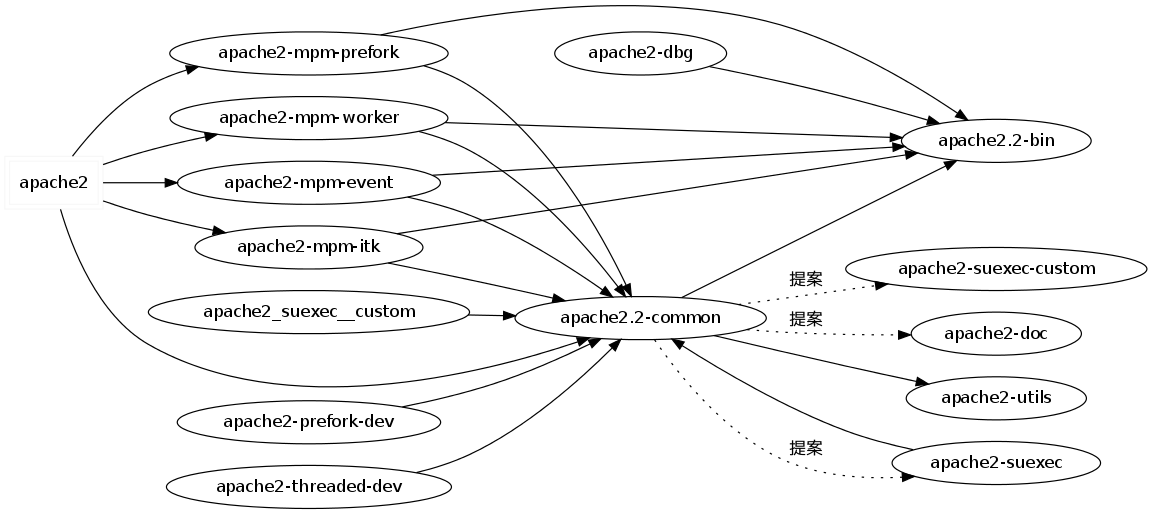
\includegraphics[width=1.0\hsize]{image201203/apache2-pkg.png}
 \end{center}
\label{fig:apache-pkg-dep}\caption{Debian でのパッケージ依存関係}
\end{figure}

\subsubsection{インストール}

Debianで Apache2 をインストールする場合は \texttt{apt-get install}コマンドを
使います(図\ref{fig:install})。

Debianでは apache2 というメタパッケージを使ってインストールすることが多いです。
apache2 をインストールすると、apache2-mpm-worker がインストールされます。
他の HTTP サーバパッケージをインストールしたい場合は、各々のパッケージを
指定してインストールする必要があります。

またCentOSなどでは、「httpd」 パッケージとして提供されているのでパッケージ名が異なります。
普段は他のディストリビューションを使っている人は注意しましょう。


\begin{figure}[ht]
 \begin{center}

\begin{commandline}
$ sudo apt-get update          // リポジトリを更新
$ sudo apt-get install apache2 // apache2 パッケージをインストール
\end{commandline}
%$

 \end{center}
\label{fig:install}\caption{Debian で Apache2 をインストールする}
\end{figure}

\subsubsection{Apache HTTP サーバの起動と停止}

Debian は「インストールしたものは使う」というポリシーなので、インストール完了の時点で
既に Apache HTTP サーバは起動しています。停止したい場合には root 権限で
「\texttt{/etc/init.d/apache2 stop}」 を実行します。
起動したい場合は 「\texttt{/etc/init.d/apache2 start}」、再起動したい場合には
「\texttt{/etc/init.d/apache2 restart}」を実行します。
図\ref{fig:startstop}に例を示します。

\begin{figure}[ht]

\begin{commandline}
$ ps ax | grep apache2 // apache2 のプロセスを確認
10034 ?        Ss     0:05 /usr/sbin/apache2 -k start
13008 ?        S      0:00 /usr/sbin/apache2 -k start
(省略)
$ sudo /etc/init.d/apache2 stop // apache2 を停止
$ ps ax | grep apache2 // apache2 のプロセスを確認
16833 pts/1    S+     0:00 grep apache2
$ sudo /etc/init.d/apache2 start //apache2 を開始
10048 ?        Ss     0:05 /usr/sbin/apache2 -k start
13024 ?        S      0:00 /usr/sbin/apache2 -k start
(省略)
\end{commandline}

\label{fig:startstop}\caption{Apache2の起動と停止}
\end{figure}

デフォルトの状態では、マシンを立ち上げ時に HTTP サーバが起動するようになっています。
マシン立ち上げ時に HTTP サーバの起動しないようにするには、ランレベル毎のサービス起動スクリプト
を制御するツール \texttt{update-rc.d}を使います。

全てのランレベルで apache2 を起動させないようにするには、コマンドに
サービス名と remove を指定して実行します。
またインストール直後のデフォルトの状態に戻したい場合には、コマンドに
サービス名と default を指定して実行します。実行例を図\ref{fig:update-rc}に示します。

\begin{figure}[ht]
\begin{commandline}
$ sudo update-rc.d -f apache2 remove // 全てのランレベルで apache2 を起動させないようにする
$ sudo update-rc.d -f apache2 default //サーバ起動をデフォルトの状態に戻す
\end{commandline}
%$
\label{fig:update-rc}\caption{ランレベルの制御}
\end{figure}

Red Hat系では \texttt{chkconfig}を使いますが、Debianでも提供されています。
しかし、chkconfig は RedHat系のサービス管理ツールなので Debian
ではうまく動作しないことがあるようです。同様のツールとして
\texttt{sysv-rc-conf}があるのでこちらを使ったほうがいいでしょう。
図\ref{fig:sysv-rc}に簡単な使い方を説明します。

\begin{figure}[ht]

\begin{commandline}
$ sudo apt-get install sysv-rc-conf // sysv-rc-conf パッケージをインストール
$ sudo sysv-rc-conf --list // 現在の状態を出力
apache2      0:off1:off2:on3:on4:on5:on6:off
bootlogd     S:on
(中略)
$ sudo sysv-rc-conf --level 2 apache2 off // ランレベル2のapache2を無効にする
$ sudo sysv-rc-conf --list | head -1 // 現在の状態を出力
apache2      0:off1:off2:off3:off4:off5:off6:off
$ sudo sysv-rc-conf --level 2 apache2 on // ランレベル2のapache2を有効にする
$ sudo sysv-rc-conf --list | head -1  // 現在の状態を出力
apache2      0:off1:off2:on3:off4:off5:off6:off
\end{commandline}
%$
\label{fig:sysv-rc}\caption{Apache2の起動と停止}
\end{figure}


\subsection{Apache2 の設定ファイル}

Red Hat 系の場合、主な設定は \texttt{/etc/httpd/conf/httpd.conf}で行い、include されるファイルは
\texttt{/etc/httpd/conf.d/}ディレクトリに格納しますが、Debian の場合は表\ref{tab:apache-files}のように
なっています。

\begin{table}[ht]
\begin{center}
\begin{tabular}{|l|l|}
\hline
設定ファイル & 内容\\
\hline \hline
/etc/apache2/apache2.conf & 基本設定\\
\hline
/etc/apache2/httpd.conf & オーバーライドする設定\\
\hline
/etc/apache2/conf.d/ & 基本設定の中でIncludeするファイルを格納する\\
\hline
/etc/apache2/ports.conf & ポートの設定\\
\hline
/etc/apache2/envvars & 環境変数の設定\\
\hline
/etc/apache2/mods-available/ & 利用可能なモジュール設定\\
\hline
/etc/apache2/mods-enabled/ & 利用中のモジュール設定\\
\hline
/etc/apache2/sites-available/ & 利用可能なサイト設定\\
\hline
/etc/apache2/sites-enabled/ & 利用中のサイト設定\\
\hline
/var/www & ドキュメントルート\\
\hline
/usr/lib/cgi-bin & cgi-bin\\
\hline
/var/log/apache2 & Apache2 ログ\\
\hline
\end{tabular}
\caption{\label{tab:apache-files}{Debian の Apache2 設定ファイル群}}
\end{center}
\end{table}

\texttt{apache2.conf}には図\ref{fig:apache2conf}のような行があり、\texttt{apache2.conf}
から各設定が読み込まれるようになっています。
Apache2 の設定を
を変更する場合、\texttt{apache2.conf}を変更せず、
\texttt{httpd.conf} や \texttt{ports.conf}を変更します。

\begin{figure}[ht]
\begin{commandline}
(省略)
# Include module configuration:
Include /etc/apache2/mods-enabled/*.load
Include /etc/apache2/mods-enabled/*.conf

# Include all the user configurations:
Include /etc/apache2/httpd.conf

# Include ports listing
Include /etc/apache2/ports.conf
(中略)
# Include generic snippets of statements
Include /etc/apache2/conf.d/

# Include the virtual host configurations:
Include /etc/apache2/sites-enabled/
\end{commandline}

\label{fig:apache2conf}\caption{apache2.confの内容}
\end{figure}


\subsection{サイトを設定する}

Debian は\texttt{/etc/apache2/sites-available/default} に apache2 のデフォルトのサイト設定
を格納しています。サイトを一つだけ構築する場合はこのファイルを変更し、
apache2 を再起動すれば
設定された内容で apache2 が立ち上がります。再起動する方法は図\ref{fig:apache2restart}の通りです。

\begin{figure}[ht]
\begin{commandline}
$ sudo /etc/init.d/apache2 restart
\end{commandline}
%$
\label{fig:apache2restart}\caption{Apache2の再起動}
\end{figure}

Debian の apache2 で複数のサイトを立ち上げる場合、httpd.conf や apache2.conf は編集しません。
サイト別に設定を記述し、\texttt{/etc/apache2/sites-available/}ディレクトリに格納します。
そして、そのサイトを設定を有効にするコマンド「\texttt{a2ensite}」実行し、apache2 を再起動します。

簡単な手順を説明します。
例えば、test.example.org というサイトを立ち上げるとします。内容は図\ref{fig:siteexample}のようになるでしょう。

\begin{figure}[ht]
\begin{commandline}
<VirtualHost *>
    ServerAdmin admin-test@example.org
    ServerName test.example.org
    DocumentRoot /home/test/public_html/
    <Directory />
        Options FollowSymLinks ExecCGI Includes
        AllowOverride None
    </Directory>
</VirtualHost>
\end{commandline}
\label{fig:siteexample}\caption{サイトの設定例}
\end{figure}

そしてこのサイト設定を\texttt{/etc/apache2/sites-available/test}に格納します。
格納した後、サイトを有効にする「\texttt{a2ensite}コマンド」に有効にしたいサイトの
設定ファイル名を指定して実行します。実行すると\texttt{/etc/apache2/sites-enabled/}
にシンボリックリンクが張られ設定が有効になります。
有効にしただけでは、稼働しているhttpd サーバには設定が反映されていないため、
httpd サーバを再起動します(図\ref{fig:siteenable-setting})。

\begin{figure}[ht]
\begin{commandline}
$ ls -l /etc/apache2/sites-enabled/
合計 0
lrwxrwxrwx 1 root root 26 2011-03-20 08:23 000-default -> ../sites-available/default
lrwxrwxrwx 1 root root 30 2011-03-20 08:23 default-ssl.old -> ../sites-available/default-ssl
$ sudo a2ensite test // test を有効にする
Enabling site test.
Run '/etc/init.d/apache2 reload' to activate new configuration!
$ ls -l /etc/apache2/sites-enabled/
合計 0
lrwxrwxrwx 1 root root 26 2011-03-20 08:23 000-default -> ../sites-available/default
lrwxrwxrwx 1 root root 29 2012-03-10 06:24 test -> ../sites-available/test
lrwxrwxrwx 1 root root 30 2011-03-20 08:23 default-ssl.old -> ../sites-available/default-ssl
$ sudo /etc/init.d/apache2 restart // Apache2 を再起動
\end{commandline}
\label{fig:siteenable-setting}\caption{サイトを有効にする}
\end{figure}

サイトの設定を無効にする場合には、サイトを有効にする「\texttt{a2dissite}コマンド」
に無効にしたいサイトの設定ファイル名を指定して実行します。実行すると\texttt{/etc/apache2/sites-enabled/}
からシンボリックリンクが削除されます。サイト設定を無効にした後は、有効時と同様にhttpd サーバを
再起動する必要があります(図\ref{fig:sitedisable-setting})。

\begin{figure}[ht]
\begin{commandline}
$ sudo a2dissite test // test を無効にする
Site test disabled.
Run '/etc/init.d/apache2 reload' to activate new configuration!
$ ls -l /etc/apache2/sites-enabled/
合計 0
lrwxrwxrwx 1 root root 26 2011-03-20 08:23 000-default -> ../sites-available/default
lrwxrwxrwx 1 root root 30 2011-03-20 08:23 default-ssl.old -> ../sites-available/default-ssl
\end{commandline}
%$

\label{fig:sitedisable-setting}\caption{サイトを無効にする}
\end{figure}

このように Debian ではサイトの設定を分離し、サイト毎に状態を管理することができます。
他のディストリビューションでは \texttt{include} 等を使って管理することができますが、
ファイル内容を変更する必要があり非常に手間です。
Debian はシンボリックリンクを使うことによってApache2 の設定ファイルを
変更せずにサイト設定の有効・無効ができるようになっています。

\subsection{モジュールを有効/無効にする}
Debian のモジュールに関する設定はモジュール毎の設定ファイルとして
\texttt{mods-available}ディレクトリに格納されています。
それらのうち、実際に有効にするものが
シンボリックリンクとして \texttt{mods-enabled} ディレクトリに張られます。
シンボリックリンクは手動で行わず、モジュールを有効にする場合には\texttt{a2enmod}コマンド、
無効にする場合には\texttt{a2enmod}コマンドを使います。図\ref{fig:a2enmod}にmod\_info を有効にする例とmod\_info を有効にする例を示します。

\begin{figure}[ht]
\begin{commandline}
$ sudo a2enmod info // mod_infoを有効にする 
$ sudo a2dismod info // mod_infoを無効にする
\end{commandline}
%$
\label{fig:a2enmod}\caption{mod\_infoを有効にする・mod\_infoを無効にする}
\end{figure}

\subsection{その他}

その他、注意すべき点をいくつか教えてもらったので紹介します。

\subsubsection{libapache2-mod-php5 と apache2-mpm-prefork}

Apache2 上で mod-php5 を使いたい場合、apache2-mpm-worker は使えない点に
注意してください。これは PHP5(mod-php5)の制限で、スレッドで動作することができないためです。
libapache2-mod-php5 をインストールすると、
を使いたい場合、apache2-mpm-worker が削除され、apache2-mpm-prefork がインストールされます。
PHP ユーザの方は注意しましょう。

\subsubsection{再起動確認について}
その他、Debian で Apache2 を使う理由として、再起動確認を行うという点があります。
例えばglibc が更新されたとき、サーバ系は再起動する必要があるのですが、Red Hat系では
再起動してくれず、管理者が手動で行う必要があります。
CentOS を使っている会社ではデーモンを再起動しないとならないアップデートがあったかどうか
チェックするツールをわざわざ作って管理していたりするようです。
しかし Debian では再起動の確認が行われる(設定によって自動再起動も可能)ので、
管理者の手を煩わせません。このような細かいところに気を使ってくれるのも Debianの良い所です。

\subsection{まとめ}
Debian のパッケージ古いというのは昔の話です。
stableとtesting へのセキュリティバグへの対応があり、その対応も他のディストリビューションと
比べて比較的早いです。
よく指摘されるDebian の設定ファイル、ディレクトリ構造ですが、
今回の説明で独自なのは理由があり、理にかなっている事が分かります。
またこれらを容易に操作できるように、専用のツールもあります。
パッケージによる、細かいところへの気配りができるところがDebianのよいところだと思います。
今回のApache の話が気になった方はとりあえずDebian 使ってみてはいかがでしょうか。

%-------------------------------------------------------------------------------
\dancersection{Debian での node 入門}{上川純一}
%-------------------------------------------------------------------------------
\index{node.js}
\index{node}
\index{javascript}

JavaScript\cite{javascript-mdn,ecmascript}で
プログラムをガリガリ書きたいとおもったことはありませんか?
昨年(2011年)一時期話題になっていたnodeをDebianで試してみましょう。
node\footnote{マニュアルなどにはnodeと記述されていますが、通称は
node.jsのようです}は
イベントベースのサーバサイドJavaScriptエンジンとフレームワークです。
何に使えるかというと、JavaScriptでウェブサーバが書きやすくなっています。
シェルスクリプトでコードを書く代わりにnodeを使ってJavaScriptを使うことも
まぁ出来ますがウェブサーバが便利になるのが一番大きいと思われます。
特徴はシングルスレッドなんだけどほとんどすべてのI/O処理を非同期イベント
処理によって実現することによって、たくさんのリクエストを効率よく処理する
あたりでしょうか。

node のパッケージはsqueezeにはないですが、wheezy にはすでに入っていま
す。
インストールは簡単:
\begin{commandline}
# apt-get install nodejs
\end{commandline}

Node 本体は nodejs というパッケージ名で入っています\footnote{すでにnodeと
いうパッケージが存在するからnodeという名前がつけられなかったのだと思われ
ます。}が、関連するモジュールパッケージの名前はnode-ではじまるようになっ
ています。

node コマンドを実行するとJavaScriptインタープリタのREPLインタフェースが起
動します。ここでコマンドラインからJavaScriptを適当に実行できるようです。
この時点では単なるV8のコマンドラインインタフェースですね。

\begin{commandline}
$ node -v
v0.6.12
$ node
> console.log('hello world')
hello world
\end{commandline}

nodeのバージョン番号ですが、node の2012年4月1日時点の安定版の最新版は0.6
系列で、0.7系列は開発版という位置づけのようです。0.8系列がリリースされた
らまたDebianのnodeも更新されるでしょう。

まとめると次のようになっています。
\begin{itemize}
 \item 0.4: 2012年1月までDebian sid に入っていた安定版
 \item 0.6.12: 2012年4月時点での最新安定版(stable)
 \item 0.7.x: 開発版(unstable)
 \item 0.8.x: 多分近い将来リリースされるだろう安定版
\end{itemize}

\subsection{Debian 流儀でのNodeモジュールパッケージインストール}

Debianパッケージで提供されている node のモジュールパッケージを使ってみましょう。

\subsubsection{NodeでCLIツールを作ってみる}

とりあえず、node でコマンドラインインタフェース(CLI)のツールをつくってみたい、のでnode cli を
インストールして適当にコードを書いてみるという場面を想定してみます。cli
モジュールはDebianパッケージになっているので以下でインストールできます。
\index{node-cli}

\begin{commandline}
# apt-get install node-cli
\end{commandline}

とりあえず無駄に平均を計算してみるコードを書いてみました。

\begin{commandline}
// Command-line tool to sum the stdin items.
var cli = require('cli');

cli.withStdinLines(function(lines, newline) {
    var sum = 0;
    var count = 0;

    for (var i = 0; i < lines.length; ++i) {
	console.log(lines[i]);
	if (lines[i] != '') {
	    sum += parseInt(lines[i]);
	    count ++;
	}
    }
    console.log('sum: ' + sum + ' avg: ' + sum / count);
});
\end{commandline}

コマンドラインで適当に実行してみたところ、結果が表示されました。

\begin{commandline}
$ node sum.js < testdata.txt
10
15
200
8

sum: 233 avg: 58.25
\end{commandline}
%$
\subsection{npm -- Node のパッケージ管理システム}
\index{npm}

Node のモジュールは npm で管理されています。Debian パッケージになって
いないパッケージなどは、npm コマンドを利用して直接インストールすることも可能です。
Perl でいうCPAN、TeXでいうCTAN のようなもののようです。
Debian パッケージを使うべきかnpmを使って導入するべきか悩ましいところです
が、Debianパッケージになるまでにはどうしてもタイムラグがあるので、最新のコードをつ
かって開発する場合にはnpmを利用することになると思われます。ある程度こな
れてきたらないパッケージはITPするのがよいでしょう。

Debianの提供するモジュールパッケージは/usr/lib/nodejs 以下にインストール
されますが、
Debian パッケージの npmを利用する場合は /usr/local/lib/nodejs 以下に入り
ます。

で、喜び勇んで手元で実行したところExceptionをはいて終了しました。どうやら
node 0.6.2に対応していない古いバージョンの npm (Node 0.4系列ではうごいた
はず)が現在パッケージされており、動かなくなっている模様です。
\debianbug{622628}

\subsection{npmのアップストリーム版をインストールしてみる}

npmが使えないのは不便なので、Debianパッケージになっていないnodeモジュール
をインストールする方法としてDebianパッケージではないnpmを利用する方法を紹
介します。

node 0.6 系列に対応しているnpmは1.1です。
npmjs\cite{npmjs} サイトからインストーラをダウンロードして実行します。
npm がインストールできたらモジュールは npm installコマンドでインストールできるよ
うになります。
\index{npm install}

npm は sudo 前提で設計されているようです。sudoでroot権限に昇格するのはビ
ルド時にnobody権限に切り替えるのに使うようです。

npmパッケージはシステムグローバルにもパッケージローカルにもインストールで
きますが、一般ユーザ権限でプロジェクトローカルに利用するためにパッケージ
をインストールすることを基本として設計されているようです。

\texttt{sudo npm install パッケージ名}
だとカレントディレクトリ以下にsudoを発行したユーザ権限でインストールする
ようです。\footnote{ビルド自体はnobody権限で行うようです}
\texttt{sudo npm install -g パッケージ名} だと \verb!/usr/lib/node_modules! 以下にインストール
するようですが、権限はnobodyのままです\footnote{挙動としてはおかし
いので操作を間違っているかバグのように思われる}。

npmは開発者視点で便利なように設計されているようで、個人的におもしろいなと思った
のは -g をつけずに \texttt{sudo npm install} だけすると現在のディレクトリにあるプロジェ
クトの依存しているパッケージをカレントディレクトリにインストールするとい
う挙動になることです。依存しているパッケージがどんどん変更されている
熱いプロジェクトであるnodeっぽい感じがします。
npmの作者のウェブサイトを読んでいると、システムワイドでインストールする
のはCLIツールなどに必要な時に限って、ウェブサイトにデプロイする用のコー
ドではモジュールはプロジェクトのディレクトリにインストールすることを推奨
すると説明しています。

\begin{commandline}
# apt-get install nodejs nodejs-dev
# curl http://npmjs.org/install.sh | sh
$ sudo npm install -g express ejs socket.io
npm http GET https://registry.npmjs.org/express
npm http GET https://registry.npmjs.org/ejs
npm http GET https://registry.npmjs.org/socket.io
npm http 304 https://registry.npmjs.org/socket.io
npm http 200 https://registry.npmjs.org/ejs
npm http GET https://registry.npmjs.org/ejs/-/ejs-0.6.1.tgz
npm http 200 https://registry.npmjs.org/express
  .
  .
/usr/bin/express -> /usr/lib/node_modules/express/bin/express
ejs@0.6.1 /usr/lib/node_modules/ejs
express@2.5.8 /usr/lib/node_modules/express
├── qs@0.4.2
├── mkdirp@0.3.0
├── mime@1.2.4
└── connect@1.8.6
socket.io@0.9.2 /usr/lib/node_modules/socket.io
├── policyfile@0.0.4
├── redis@0.6.7
└── socket.io-client@0.9.2
\end{commandline}
%$

ディレクトリ構成をまとめました。

\begin{table}[h]
\caption{Debianパッケージおよびnpm でインストールされる場所}
\begin{center}
 \begin{tabular}{|l|l|}
 \hline
 & ディレクトリ\\
 \hline
 Debian パッケージ & \texttt{/usr/lib/nodejs} \\
 Debian の npm  & \texttt{/usr/local/lib/nodejs}\\
 npm install -g & \texttt{/usr/lib/node\_{}modules} \\
 npm install & \texttt{./node\_{}modules} \\
 \hline
 \end{tabular}
\end{center}
\end{table}

マニュアルなどはnpm コマンドを実行すると表示されるヘルプが充実しています。
\begin{commandline}
$ npm help
$ npm help npm
$ npm help install
\end{commandline}
%$ -- for emacs

\subsubsection{npm を使っている場合のプログラム実行}

カレントディレクトリにインストールしたときはよいのですが、そうではない場
合は、\texttt{/usr/lib/node\_{}modules}以下にインストールされてもDebianの
nodejs の標準のモジュールパスに含まれていないためモジュールがロードされません。

ひとつの回避策としてはモジュールを探しに行くPATHを追加するという方法があります。
\texttt{NODE\_{}PATH}環境変数を指定すれば追加でロードされるようになりま
す。
\index{NODE\_{}PATH}
\begin{commandline}
$ NODE_PATH=/usr/lib/node_modules node ./program.js
\end{commandline}
%$ -- for emacs

\subsubsection{パッケージのメタデータ: package.json}

推奨されているのはパッケージに必要なモジュールをpackage.json に記述して、
\index{npm link}
npm link コマンドを実行すればパスの追加は必要なくなります。
\begin{commandline}
$ npm link
\end{commandline}
%$
とすると必要なモジュールをプロジェクトのディレクトリの
\texttt{./node\_{}modules}にリンクしてくれるということでした。
\footnote{マニュアルにはシンボリックリンクをすると書いているけど、モジュー
ルはハードリンクしてました。}
\footnote{逆方向に現在作業中のパッケージを/usr/lib/node\_{}modules/以下
にシンボリックリンクしてくれます。作業した内容がすぐに反映するので便利と
いえば便利。}

\index{package.json}
npmのメタデータは ./package.json です。
npm help json (man npm-json.1)に詳しく説明されています。
す。とりあえずはname/versionフィールドさえあればよくて、dependenciesを追
加するとnpm install やnpm link コマンドで利用してくれるようです。

インストールに必要なファイルの一覧や、node-waf の実行方法などが記載され
ているのでこれさえあればDebianパッケージを自動で生成することも可能な気が
します。

手元で作成してみた npm linkのためだけの最低限な内容のpackage.jsonを紹介
します

\begin{commandline}
{
    "name": "aptserver",
    "version": "v0.0.1",
    "dependencies": {
	"cli": "",
	"express": "",
	"ejs": ""
    }
}
\end{commandline}


\subsection{とりあえず簡単なサーバを書いてみた}

apt-cache search をして出力を返すだけの簡単なサーバを書いてみました。
イベントドリブンな部分としては、HTTP requestのハンドラーをapp.get() で登
録している部分と、apt cache の出力を aptCache.stdout.on で登録したハンド
ラーで取得して aptCache.on exit ハンドラーで終了したらHTTPレスポンスを返
すようになっている部分でしょうか。

書いてみて気づきましたが、いまいちnodeを使うメリットが出てないきもしま
す。


\begin{commandline}
/*
 * A simple server which serves apt cache search results.
 */
var child_process = require('child_process');
var cli = require('cli');
var url = require('url');
var ejs = require('ejs');

cli.parse({
    port: ['p', 'HTTP server will listen on this port.', 'number', 8088]
});

cli.main(function cliMain(args, options) {
    var express = require('express');
    var app = express.createServer();
    // set view options.
    app.set('view engine', 'ejs');
    app.set('view options', { layout: false });
    app.set('views', __dirname + '/views');

    // Set up routes.
    app.get('/', getSlash);
    app.get('/search', getSearch);

    console.log('Start listening on http://localhost:' + options.port + '/');
    app.listen(options.port);
});

/** handler for '/' request */
function getSlash(request, response) {
    response.render('index.ejs');
}

/** handler for '/search?' request */
function getSearch(request, response) {
    var query = request.query.q;
    var aptCache = child_process.spawn('apt-cache',
				       [ 'search', query ]);
    /** Output of apt-cache search, to be used for response. */
    var responseString = '';
    aptCache.stdout.on('data', function handleAptCacheStdout(data) {
	responseString += data;
    });
    aptCache.stderr.on('data', function handleAptCacheStderr(data) {
	responseString += data;
    });
    aptCache.on('exit', function handleAptCacheExit(exitCode) {
	// apt-cache finished executing, send repsponse back to the server.
	response.render('search.ejs',
			{locals:{query: query,
				 response: responseString}});
    });
}
\end{commandline}

ejs HTMLテンプレートファイル\texttt{views/search.ejs}はこんな内容になり
ました。

\begin{commandline}
<!-- -*- html; -*- -->
<html>
  <body>
    <form
      method=GET
      action='/search'>
      <input type=text name=q></input>
      <button>search</button>
    </form>
    <h3>Search for: <%= query %></h3>
    <pre>
<%= response %>
    </pre>
  </body>
</html>
\end{commandline}

追加モジュールはexpress, ejs, cli を使いました。それぞれを簡単に紹介する
と以下です

\begin{itemize}
 \item express: ウェブアプリケーションフレームワークとしてnodeで最もポ
       ピュラーなモジュール、リクエストベースのルーティングなどを担当。
 \item ejs: HTMLテンプレートエンジンとしておそらく最もポピュラーなモジュール。
 \item cli: コマンドラインオプションをパースしてくれるモジュール。
\end{itemize}


\subsection{最後に}

今回は node をDebianで使う方法を紹介してみました。モジュールのパッケージ
ングが更新においついていない感じなのでもうしばらくしたらまた良くなってい
るかもしれませんが、そうこうしているうちにnode 0.8がリリースされてしまい
そうです。
node の頻繁な更新とそれによってモジュールが複数バージョン必要になってく
る現状から、nave / nvm などの環境管理ツールで複数バージョンをインストール
して利用するということもよくやられているようです。
この資料がDebianでnodeを活用するきっかけ、およびパッケージ化活動の一助になれば幸いです。

\begin{thebibliography}{0}
\bibitem{nodejslocalhtml}  Node.js v0.6.12 Manual \& Documentation
	\url{/usr/share/doc/nodejs/api/index.html}
\bibitem{pkg-javascript-devel} Alioth の  pkg-javascript-devel メーリン
	グリスト
	\url{http://lists.alioth.debian.org/pipermail/pkg-javascript-devel/}
\bibitem{npmjs} NPMホームページ \url{http://npmjs.org/}
\bibitem{debiannode} nodejs for Debian
	\url{/usr/share/doc/nodejs-dev/README.Debian}
\bibitem{javascript-mdn} JavaScript \url{https://developer.mozilla.org/ja/JavaScript}
\bibitem{ecmascript} Standard ECMA-262
ECMAScript Language Specification 5.1
\url{http://www.ecma-international.org/publications/standards/Ecma-262.htm}
\end{thebibliography}

\clearpage

%-------------------------------------------------------------------------------
\dancersection{Android機でDebian}{野島 貴英}
%-------------------------------------------------------------------------------
\label{sec:android-debian}
\index{debiandroid}
\index{Android}

\subsection{はじめに}
携帯電話、タブレット型PCなど、高性能の情報端末を持ち歩くのが一般的になってきました。
ここでは、これら情報端末のうち、Android OSを搭載した情報端末にDebianを入れ、
Debian開発者の環境を築いてみようとした事について述べます。

\subsection{材料:Android端末 Barnes \& Noble Nook Colorについて}
\index{nook color}

手頃なAndroid端末として、たまたま手元にBarnes \& Noble社(以下B\&N)の
Nook Colorという製品\footnote{\url{http://www.barnesandnoble.com/p/nook-color-barnes-noble/1100437663}}があります
\footnote{製品の写真は権利関係がよく判らないので割愛させてください。詳し
くは先のURL参照。}。
値段も日本で輸入した場合、2万円前半〜後半ぐらいで安く、電子書籍ビューアということもあり
デザインも小型でそれなりに薄く軽量です。これは元々、PDFにした
カラーの本(漫画も)を持ち歩きながら読めればと思って買っていたものでした。

これがDebianの開発環境としても動いたら素敵と思い、こちらを
早速利用する事にします。
\footnote{実は、自分はフィーチャーフォン(ガラケーともいう)しか持っておらず、Android端末はこれしか持ってなかったことは秘密です。}

\subsection{Android端末のDebian動作の方針}

Android端末を利用してDebian関係のディストリビューションのOSを動作させる場合、
後に述べる2つの方針が取れます。

\subsubsection{方針1: Android端末の機能を最大限活用する}

本方針は、Android端末はベースのOSが基本的にLinuxであることを最大限利用します。

ここで、
\begin{enumerate}
\item Android端末のCPUにあわせたDebian関係のLinuxのファイルシステムを/(ルート)ファイルシステムからSDカードや、内臓メモリへ用意します。
\item Android端末にAndroidアプリのVNC Viewer\footnote{\url{http://code.google.com/p/android-vnc-viewer/}}を搭載しておきます。
\item 何らかの方法でAndroid端末上の管理権限を奪取した状態で、先ほど用意した/ファイルシステムをマウントし、chrootします。これでDebianのバイナリが動作できるようになります。
\item 最後にDebianのバイナリを利用してvncserverを立ち上げ、AndroidアプリのVNC Viewerで127.0.0.1:5901に接続し、Debianを利用します。
\end{enumerate}
という方法がよく利用されます。

この方法は、Android端末で管理権限さえ奪取できていればDebian関係のLinuxディストリビューションを動作させる事ができます。
さらに良いことに、本体のAndroid端末が最初から搭載している無線ネットワークもそのまま利用できるるため、非常に都合が良いです。
実際、自分は未評価ですがこれらの諸々の手続きを全部アプリに詰め込んでしまったものに、

\begin{itemize}
\item Ubuntuを動作させるAndroid アプリ:ubuntu instller free \url{https://play.google.com/store/apps/details?id=com.zpwebsites.ubuntuinstall&hl=ja}
\item Debianを動作させるAndroid アプリ: Lil' Debi \url{https://github.com/guardianproject/lildebi/wiki}
\end{itemize}
などがあるようです。

% ubuntu on nook スレ
% http://forum.xda-developers.com/showthread.php?p=10306407
\subsubsection{方針2: Android OSを使わずそのままDebianをブートする}

Android端末は大抵ARMベースのCPUで動いてます。DebianもARMベースのバイナリを
用意しています。これはつまり、うまくカーネル/アプリケーションをAndroid端末の
ハードの仕様に合わせることができ、ブートさせる事ができれば、Android OSの
代わりにDebianをそのままブートさせて使えるはずです。

ただ、Android端末はARMベースのCPUは使っているものの、グラフィックス
(液晶画面出力)、タッチパネル、サウンド、Wi-Fi等は各端末のハード独自のものでかつ、
仕様/設計は未公開であったり、Linuxカーネル本体の機能だけでは対応できなかったりする為、
これらの周辺デバイスを利用できるようにする為のハードルは高い状況です。特に、
Wi-Fiはおろか、通常のデスクトップPCを使っているときにはあまりに基本的な機能で
気にもとめなかったような機能(キー入力、マウス入力、画面に文字を描画)すらも
最初から未対応がほとんどですので、本方針を取るにはそれ相応のスキルが必要です。
(VGA BIOSとか、IBM PC ATのBIOSの規格が大変ありがたく見えてきます)

但し、本方針でもしDebianをそのまま利用できれば、より自由なソフトウェア開発環境を
搭載した携帯端末を手にできる事になる為、非常に魅力的ではあります(よね?)

\subsection{数々の障害と方針変更}

先に述べた方針1が手軽なはずなので、こちらの方針をとって作業を進めていました。
が、実は以下に列挙する問題にあたってしまい、解決出来なかった為、不完全ながらも
方針2を取らざるを得ない状況となってしまいました。

\begin{enumerate}
\item B\&NのNook Colorは、Android 2.1〜2.2 OSを改造して電子書籍端末にした製品のため、通常のAndroid OSとは異なります。
そのため、Android端末でそのまま動作させることができるようなアプリをどうやってもインストールできませんでした。
つまり頼みのVNC Viewerを動作させる事が出来ませんでした。また、こちらの原因を調べようにも、ソース公開義務の発生しない
肝心のライブラリ、アプリケーションフレームワーク、アプリケーション
\footnote{Android OSの用語となります。基本的なAndroid OSの構造:\url{http://developer.android.com/images/system-architecture.jpg}}
が全くの非公開であるため原因追求が困難です。
\item 管理権限を奪取してadbが使えるようにしたのですが、USB経由で利用するNook Color側のadbdの動作が非常に不安定で、
一度でもUSBを外す/PCの電源を落とす/何もせず時間を空けると次からどうやっても端末側adbdに接続できなくなる現象に悩まされました
(管理権限奪取の方法を最初からやり直すと復活できる事がたまにありましたが、なぜか失敗する事が多いです。)
さらに悪い事に、端末側ファームを1.2.2にアップデートすると、もはやどうやってもadbdに接続できなくなってしまいました
\footnote{後の調査でわかったことですが、Wi-Fi経由で端末側adbdに接続すると安定するかも?との情報もあります。しかし、無線LAN環境を自分は持っていない為こちらも未評価です}。
\end{enumerate}

そこで、方針1をあきらめ、方針2を取る事にしました。

\subsection{再考:Nook Color}

DebianをAndroid端末の機能を最大限活用して動作させるのにいろいろてこずる
Nook Colorですが、このやり方を諦めれば、唯一Debianを動作させるのに救いのある機能があります。
Nook ColorはminiSDを挿入して利用できるのですが、ここにOMAP用ブート形式
\footnote{\url{http://processors.wiki.ti.com/index.php/SD/MMC_format_for_OMAP3_boot}。
但しこのページのコマンド通りにそのままfdisk実行しても、Debianではブートイメージは作れないので注意。}
のブートイメージを書きこんでおくと、こちらからそのままブートしてしまう機能(脆弱性?)があります。

そこで、ここにブートイメージを書き込んで、ブートすればDebianを利用できるのでは?
という事を試しました。

\subsection{DebianのNook Color用ブートイメージを作る}

\subsubsection{方針}

ここでは、以下の方針にそってブートイメージを作成します。

\begin{enumerate}
\item qemuを使ってDebianのARM用ディスクイメージを構築します。
\item Nook Colorのroot奪取に使うnooter0.2.zipのカーネル/initrdイメージはNook ColorのUSBをRNDIS用のネットワークI/Fにセットアップする能力を持ちます。これを利用すると、コミュニケーションポートとしてUSBが非常に便利になるのでこれらを拝借します。
\item 以上1,2を合体したOMAP用ブート形式のminiSDカードを作成します。
\end{enumerate}

具体的なやり方を次に述べます。

\subsubsection{やり方}

用意するもの:Debian sidの動くPC,グローバル回線, miniSDカード1枚、必要ならminiSDカー
ドリードライター(USBメモリに変換するタイプのコネクタでも可)

\begin{enumerate}
\item  諸々PC側に取り揃えます。
\begin{commandline}
$ sudo aptitude install debian-installer-6.0-netboot-armel qemu-system util-linux kpartx dump unzip gvncviewer
$ wget http://cgit.openembedded.org/openembedded/plain/contrib/angstrom/omap3-mkcard.sh; chmod 755 omap3-mkcard.sh
\end{commandline}

\item イメージディスクの準備をします。
\begin{commandline}
$ qemu-img create -f raw arm-versatile.img 5G
\end{commandline}
%$

\item インストール作業を行う為、以下のコマンドを実行します\footnote{LXDEデスクトップにする理由は、GNOMEだとメモリの必要量が多すぎてswapが発生してしまい、快適に動作しない為です}。

\begin{commandline}
$ qemu-system-arm -M versatilepb -kernel /usr/lib/debian-installer/images/armel/versatile/vmlinuz-2.6.32-5-versatile \
 -initrd /usr/lib/debian-installer/images/armel/versatile/initrd.gz -m 256 -drive file=./arm-versatile.img,if=scsi,\
 bus=0,unit=0,cache=writeback -append "root=/dev/ram desktop=lxde priority=medium"
\end{commandline}
%$

\item  Debianインストーラがウインドウに立ち上がり、通常のインストーラメニュー形式のDebianのインストールを進める事ができるようになります。ネットワークも自動的に認識(IPアドレスなども)され、qemuの持つネットワークの仕組みでPCに接続されたネットワークがそのままネットワーク経由のインストールに利用されます。表\ref{tab:armsid-ver}を選択しつつインストールを行います。

\begin{table}[ht]
\begin{center}
\begin{tabular}{|l|p{5cm}|p{5cm}|l|}
\hline
項番&設定項目&指定内容&備考\\
\hline \hline
1&Choose language & Japanese 日本語 &\\
2&ネットワークの設定 & DHCPでネットワークを自動で設定 & \\
3&インストールするDebianバージョン&sid&\\
4&ロードするインストーラコンポーネント&何も選ばない&何も選ばないが、「続ける」だけは選択\\
5&ディスクのパーティショニング&ディスク全体を使う,すべてのファイルを1つのパーティションに&\\
6&ソフトウェアの選択&デスクトップ環境、ラップトップ、標準システムの3つ& お好みで\\
7&インストールするLinuxカーネルのバージョン&3.2.0-2& \\
\hline
\end{tabular}
\caption{\label{tab:armsid-ver}インストーラで選択する項目}
\end{center}
\end{table}

\item インストールが完了し、最後にシャットダウン画面になります。最後Reboot systemの指示が出たのを確認してそのままqemuをCtrl+Cで停止させます。

\item インストール完了後のディスクイメージに内臓されているカーネルイメージ、initrdイメージを取り出します。

\begin{commandline}
$ mkdir debian
$ sudo kpartx -a ./arm-versatile.img
$ sudo mount -t ext3 /dev/mappoer/loop0p1 ./debian
$ cp debian/boot/initrd.img-3.2.0-2-versatile .
$ cp debian/boot/vmlinuz-3.2.0-2-versatile .
$ sudo umount ./debian
$ sudo kpartx -d ./arm-versatile.img
loop deleted : /dev/loop0
$
\end{commandline}
%$

\item 以下のコマンドで取り出したカーネルイメージ、initrdイメージで再度qemuを立ち上げます。xdmの画面が出るので、そのままログインします。するとLXDEのデスクトップ画面が現れます。

\begin{commandline}
$ qemu-system-arm -M versatilepb -kernel ./vmlinuz-3.2.0-2-versatile \
 -initrd ./initrd.img-3.2.0-2-versatile -m 256 -drive file=./arm-versatile.img,if=scsi,\
 bus=0,unit=0,cache=writeback -append "root=/dev/sda1 "
\end{commandline}
%$

\item LXDEの画面から、lxterminalを開き、パッケージをアップデートします。さらに、vncサーバーの導入を行っておきます。

\begin{commandline}
$ su root
Passwd: インストール時のrootパスワード
# aptitude update;aptitude safe-upgrade;aptitude install tightvncserver
\end{commandline}
%$

\item vncサーバーのインストールが完了したら、LXDE端末画面でシャットダウンします。
\begin{commandline}
$ sudo shutdown -h now
\end{commandline}
%$

\item Power offのメッセージが出力されたら、qemuをCtrl+Cで停止します。

\item miniSDをPCに差し込みます。mountされてしまっているようであれば、{\bf 必ずumount}しておきます。(注:ここでは/dev/sdb1としてマウントされてしまった事を過程します)
\begin{commandline}
$ sudo umount /dev/sdb1
\end{commandline}
%$
Tips:\\
なお、PCのminiSDのリーダ/ライターを搭載している場合、miniSDアクセス用のチップがRicho R5C822を搭載している場合で(よくある)、miniSDを挿入すると''mmc0: error -110 whilst initialising SD card''や、''mmc0: Reset 0x1 never completed''などが大量にdmesgに記録されて全くアクセスできない場合があります。この場合は以下の定義を/etc/modulesに記載してリブートすると、安定してminiSDへアクセスできるようになります。
\begin{commandline}
$ cat /etc/modules
...中略...
# for R5C822
mmc_block
tifm_sd
$
\end{commandline}

\item miniSDにOMAP用ブート形式のパーティションを作成します。\\
注:{\bf 必ずminiSDの認識されているデバイスファイルをomap-mkcard.shに指定してください!}ここでは/dev/sdbと仮定しています。間違ったデバイスファイルを指定すると該当ディスクの中身が消えてしまいます!
\begin{commandline}
$ sudo ./omap3-mkcard.sh /dev/sdb
\end{commandline}
%$

\item nooter0.2配布先(\url{http://www.mediafire.com/?cfddu9wt9d8dunl})をepiphanyなどのWEBブラウザでアクセスして、nooter0.2.zipを入手します。

\item 解凍して、ディレクトリnooter/にマウントします。
\begin{commandline}
$ unzip nooter0.2.zip
$ mkdir nooter
$ sudo kpartx -a ./nooter_sdcard_40mb.img
$ sudo mount /dev/mapper/loop0p1 ./nooter
\end{commandline}
%$

\item miniSDカードの1つ目のパーティション(/dev/sdb1)をマウントします。
\begin{commandline}
$ mkdir miniSD
$ sudo mount -t vfat -o rw,uid=your-uid,gid=your-gid /dev/sdb1 ./miniSD
\end{commandline}
%$

\item nooterのu-bootイメージ、カーネルイメージ、initrdイメージをコピーして、miniSD,nooterをアンマウントします。
\begin{commandline}
$ cp nooter/* ./miniSD/
$ sudo umount ./nooter
$ sudo kpartx -d ./nooter_sdcard_40mb.img
loop deleted : /dev/loop0
$ sudo umount ./miniSD
\end{commandline}
%$

\item miniSDの2つ目のパーティション(/dev/sdb2)をマウントして、Debianイメージをまるごとコピーします。終わったらアンマウントします。
\begin{commandline}
$ su root
Passwd:
# kpartx -a ./arm-versatile.img
# mount /dev/mapper/loop0p1 ./debian
# mount /dev/sdb2 ./miniSD
# cd debian
# dump -0 -f- ./ | (cd ../miniSD && restore -rvf- )
# cd ..
# umount ./debian
# umount ./miniSD
\end{commandline}
%$
\end{enumerate}

以上となります。

\subsection{動作させる}

早速動作させてみましょう。

\begin{enumerate}
\item Nook Colorの電源ボタンを長押しして電源をOFFにします。
\item Nook ColorのminiSDスロットに作ったminiSDを挿入します。
\item Nook Colorに製品付属のusbケーブルを差し込み、PCのUSBに差し込みます。
\item usbケーブルが橙→緑に変わる。同時にPC側のdmesgを観察すると、cdc\_etherモジュールがロードされ、usbポートがNICに変化するのが観察できます。
\item 以下のコマンドを打ち込んで、Nook Colorへrootでログインします。なお、PC側を192.168.2.10と仮決めします。(Nook Color側はnooter由来のinitrdですと192.168.2.2に決め打ちでセットアップされます。)
\begin{commandline}
$ sudo /sbin/ifconfig usb0 inet 192.168.2.10 netmask 255.255.255.0 up
$ ssh root@192.168.2.2
#
\end{commandline}
\item miniSDのDebianを動かし、vncserverを立ち上げます。
\begin{commandline}
# mount -t ext3 /dev/mmcblk0p2 /mnt
# mount -t devpts devpts /mnt/dev/pts
# mount -t proc proc /mnt/proc
# mount -t sysfs sysfs /mnt/sys
# chroot /mnt /bin/bash
root@bildroot:/# cd
root@buildroot:~# vncserver -geometry 800x600
Passwd: <適当にパスワード入れる>
Retry : <上と同じパスワード入れる>
...多少エラーメッセージが出てvncserverが立ち上がる気にしない...
root@buildroot:~#
\end{commandline}
\item PC側にてgvncviewerを起動すると、Nook Color上でDebianにログインした状態になる。
\begin{commandline}
$ vncviewer 192.168.2.2:1
\end{commandline}
%$
\item lxterminalをvncviewer上で開き、適当に/etc/resolv.confし、route add default gw 192.168.2.10等して、PC側をNAT設定にすると、
Nook ColorはUSB越しでPC側の持つグローバル側ネットワークを利用できるようになります。aptitudeなどもも全く問題なく出来ます。
\end{enumerate}

\subsection{電源の切り方}

いろいろ試したら、電源をOFFにしたくなるかと思います。この場合の手続きは以下の
通りです。

\begin{enumerate}
\item Nook Colorにsshログインします。
\item sync;sync;haltと打ち込みます。
\item Nook Colorとのsshが切れます。
\item Nook ColorからminiSDを抜きます。
\item Nook Colorの電源ボタンを15秒以上押します。
\item もう一度 Nook Colorの電源ボタンを15秒以上押すと、Nook Color本体がブートします。
あとはいつものNook Colorですので、そのまま電源ボタンを軽く押すなり放置するなりするといつも通りの電源OFF(Sleep?)状態になります。
\end{enumerate}

\subsection{終わりに}

今回手動でchrootすることにより、Nook ColorでDebianを動かしてみました。
これで電池動作で小型軽量ということもあり、Debianを入れたノートパソコンと
組み合わせると、ARM CPUのタブレット開発環境を持ち歩く事ができます。実際、
本記事を書くにあたり、平日は通勤電車の中を主に活用して試行錯誤していました。

今回Nook Colorが持っているLCD/タッチパネル/Audio/Wi-Fiについて一切
Debian側から制御までは到達できませんでした。100% Debianで動く安価で軽量な
タブレット端末の開発の道は険しそうです。

次はOMAP3用のCPU向けにkernelのクロスコンパイルに挑戦してみようかと思う
この頃でした。

\clearpage


%-------------------------------------------------------------------------------
\dancersection{Python初心者が 「Python プロフェッショナルプログラミング」 を読んでみた}{やまねひでき}
%-------------------------------------------------------------------------------
\label{sec:python-professional-programing}
\index{python}

わたくし、「Pythonプロフェッショナルプログラミング」という書籍を先日購入しました。
私自身はまだ3月末ぐらいにPythonの入門から始めたばかりで本当はPythonビギナーズプログラミングが欲しいのですが、
まだ世の中にはそのような本はありませんし、この書籍自体は評判が良かったので…。

で、実際読んでみて中々実践的というか環境構築などで参考になることが多々ありました。
しかし、もうちょっと突っ込んでみたいなぁ、というところがいくつかあったので、Debianパッケージ方面からの見方として
取り上げてみようと思います。この書籍自体ではUbuntu11.10を使っていますが、私のDebian unstableのやり方でも大体のと
ころはそのまま応用が効くはずです。


\subsection{なるべくディストリビューションのパッケージを使いたい}

PythonにはPythonパッケージがあり、配布サイトPyPIがあります。PerlにCPAN、Rubyにgems、RにCRANみたいなものですね。
で、このPythonパッケージを導入するのにpipというツールを使う旨説明があるのですが(P.4)、githubからwgetして、
インストールスクリプトをsudoで実行しています。\verb!/usr/local! 以下にツールが入るわけです。書籍全体でこのpipを
使ったインストールを勧めていますが、これは美しくない。Debianパッケージにpython-pipがあるので、そちらを入れても
いいんじゃないかと思います
\footnote{pipは若干バージョンが古いですが、そんなに不都合もないかなーと。古いのが嫌ならローカルにアップデートパッケージ作っちゃうのが吉。}。
それからユーザーの HOME 以下にパッケージをインストールするvirtualenvというツールがあります。
これもpython-virtualenvパッケージを入れて対応します。この後は、virtualenvでユーザーのPython環境にpipでパッケージを入れていってもいいかな、と思います。
便利ツールとして紹介されているvirtualenvwrapperもvirtualenvwrapperパッケージがありますのでそれを入れちゃいましょう。

\begin{commandline}
$ sudo apt-get install python-pip python-virtualenv virtualenvwrapper
\end{commandline}
%$

この後でユーザー個人のPython仮想環境下にpipでPythonパッケージをガシガシ入れていくのはありだと思います。

\subsection{複数バージョンのPythonを使う、のはいいけど。}

Python2.5をインストールするのに公式のパッケージリポジトリからだと11.10に入れられないよ、ということが書いてあります(P.11)。
ここでPPAからインストールするか、ソースからインストールするかという選択になっています。業務で使う場合、そのPPAがどれほど
信用できるかを説明するのが難しいように思います。自己責任で、って書いてありますが、大抵盲目的にそのPPA信用しちゃうような…。
古いバージョンを使わなきゃダメ、という場合、私だったら「debootstrapで古い環境を作る」というやり方でやります(debootstrapについては後ほど述べます)。

それからソースからPython2.5を入れる説明ですが、

\begin{commandline}
$ wget http://www.python.org/ftp/python/2.5.6/Python-2.5.6.tgz
$ tar -xvzf Python-2.5.6.tgz
$ cd Python-2.5.6
$ LDFLAGS="-L/usr/lib/x86_64-linux-gnu" ./configure
$ make
$ sudo make install
(「Pythonプロフェッショナルプログラミング」より引用)
\end{commandline}
%$

という説明になっています。i386だとパス変わるよね…というのは読み取れるのか若干心配な所です。プロフェッショナルだからいいのかな?
必要な依存パッケージについては、最初の方のページで

\begin{commandline}
$ sudo aptitude -y install build-essential
$ sudo aptitude -y install libsqlite3-dev
$ sudo aptitude -y install libreadline6-dev
$ sudo aptitude -y install libgdbm-dev
$ sudo aptitude -y install zlib1g-dev
$ sudo aptitude -y install libbz2-dev
$ sudo aptitude -y install sqlite3
$ sudo aptitude -y install tk-dev
$ sudo aptitude -y install zip
(「Pythonプロフェッショナルプログラミング」より引用)
\end{commandline}
%$ -- for emacs

となっていました。あぁ、これはイケてない。パッケージビルド用のパッケージ取得は apt-get build-dep するべきです。
Squeezeではまだ2.5のバイナリパッケージが手に入るので、ここでは2.4をターゲットに作業してみましょう。
こんな風に\footnote{ここのパッケージ名指定は、本当はpython2.4にしたいけど無いので2.5にしています。多少の差は後で修正。}。

\begin{commandline}
$ sudo apt-get build-dep python2.5
\end{commandline}
%$

これでPythonをビルドするときに必要な依存パッケージはすべてインストールされます。あ、apt lineにdeb-srcラインを追加を忘れずに。
このやり方なら、Python以外のソフトウェアパッケージでもバージョンが変わっても大体応用が効きます。

そして「ソースからそのまま入れると\verb!/usr/local!以下に入るから、pythonとだけ打つとPATHの優先度でソースから入れたPython2.5が起動する」…という
説明が…そんな罠作らない方がいいじゃないですかー。私ならソースから入れるのなら「Python2.5のDebianパッケージを利用環境
用にリビルドしていれる」をやります。PTSのPython2.4のページ \footnote{\url{http://packages.qa.debian.org/p/python2.4.html}}
からソースパッケージのdscファイルが取得できるので、これをdevscriptsパッケージのdgetコマンドで取得します。

\begin{commandline}
$ sudo apt-get install devscripts
$ dget http://cdn.debian.net/debian//python2.4_2.4.6-1+lenny1.dsc
dget: retrieving http://cdn.debian.net/debian//python2.4_2.4.6-1+lenny1.dsc
--2012-05-04 03:59:21--  http://cdn.debian.net/debian//python2.4_2.4.6-1+lenny1.dsc
Resolving cdn.debian.net... 150.65.7.130
Connecting to cdn.debian.net|150.65.7.130|:80... connected.
HTTP request sent, awaiting response... 404 Not Found
2012-05-04 03:59:22 ERROR 404: Not Found.

dget: wget python2.4_2.4.6-1+lenny1.dsc http://cdn.debian.net/debian//python2.4_2.4.6-1+lenny1.dsc failed
\end{commandline}
%$

あれ、oldstableだとリンクが切れちゃいますか\footnote{これはバグ報告しましょう}。しょうがないので、archive.debian.orgに切り替えてみます。
\begin{commandline}
$ dget http://archive.debian.org/debian/pool/main/p/python2.4/python2.4_2.4.6-1+lenny1.dsc
\end{commandline}
%$ -- for emacs

これでPython2.4のソースパッケージが取得できました。ビルド用の依存パッケージは既に入れているので、ソースパッケージのchangelogに
一言書いてビルドすれば独自リビジョンをつけた deb パッケージが出来上がりますので、dpkgで入れちゃえば良いでしょう(後で述べますがaptを使ってインストールも可能です)。

\begin{commandline}
$ dpkg-source -x python2.4_2.4.6-1+lenny1.dsc
$ cd python2.4-2.4.6/
$ export DEBFULLNAME="Hideki Yamane"
$ export DEBEMAIL="henrich@debian.org"
$ dch --bpo "rebuild package for my own environment"
$ debuild -us -uc
dpkg-checkbuilddeps: Unmet build dependencies: libreadline5-dev tk8.4-dev libdb4.5-dev emacs22
dpkg-buildpackage: warning: Build dependencies/conflicts unsatisfied; aborting.
\end{commandline}
%$

あれ、依存関係が満たせない。python2.5と比較してちゃちゃっと変更しましょうか。apt-get source python2.5 として、diff取ります。

\begin{commandline}
--- python2.4-2.4.6/debian/control	2012-05-04 04:09:00.000000000 +0000
+++ python2.5-2.5.5/debian/control	2012-05-04 04:13:06.000000000 +0000
@@ -1,82 +1,96 @@
-Source: python2.4
+Source: python2.5
 Section: python
 Priority: optional
 Maintainer: Matthias Klose <doko@debian.org>
-Build-Depends: debhelper (>= 5), autoconf, libreadline5-dev, libncursesw5-dev (>= 5.3), tk8.4-dev, libdb4.5-dev, zlib1g-dev,
libgdbm-dev, blt-dev (>= 2.4z), libssl-dev, sharutils, libbz2-dev, libbluetooth-dev [!hurd-i386 !kfreebsdi386
!kfreebsd-amd64], locales, mime-support, libgpm2 [!hurd-i386 !kfreebsd-i386 !kfreebsd-amd64], netbase, lsb-release, bzip2
-Build-Depends-Indep: libhtml-tree-perl, texlive-latex-recommended, texinfo, emacs22, debiandoc-sgml
-Build-Conflicts: tcl8.3-dev, tk8.3-dev, python2.4-xml, python-xml
-XS-Python-Version: 2.4
-Standards-Version: 3.8.0
+Build-Depends: debhelper (>= 5), autoconf, libreadline-dev, libncursesw5-dev (>= 5.3), tk8.5-dev, libdb4.8-dev, zlib1g-dev,
libgdbm-dev, blt-dev (>= 2.4z), libssl-dev, libbz2-dev, libbluetooth-dev [!hurd-i386 !kfreebsd-i386 !kfreebsd-amd64],
locales [!avr32 !m68k], libsqlite3-dev, libffi-dev (>= 3.0.5-2), mime-support, libgpm2 [!hurd-i386 !kfreebsd-i386
 !kfreebsd-amd64], netbase, lsb-release, bzip2, netbase, sharutils
+Build-Depends-Indep: libhtml-tree-perl, texlive-latex-recommended, texinfo, emacs23, debiandoc-sgml, latex2html
+Build-Conflicts: tcl8.4-dev, tk8.4-dev, tcl8.3-dev, tk8.3-dev, python2.5-xml, python-xml
+XS-Python-Version: 2.5
+Standards-Version: 3.9.1
\end{commandline}

debian/changelog ファイルはこんな感じにしておきましょう。

\begin{commandline}
python2.4 (2.4.6-1+lenny1~bpo60+0.1) squeeze-backports; urgency=low

  * Rebuild for squeeze-backports.
    - debian/control
     + set Build-Depends: libreadline-dev, tk8.5-dev, libdb4.8-dev
     * set Build-Depends-Indep: emacs23
  * rebuild package for my own environment

 -- Hideki Yamane <henrich@debian.org>  Fri, 04 May 2012 04:16:39 +0000
\end{commandline}

\begin{commandline}
$ debuild -us -uc
$ ls ../*.deb
../idle-python2.4_2.4.6-1+lenny1~bpo60+0.1_all.deb
../python2.4-dev_2.4.6-1+lenny1~bpo60+0.1_amd64.deb
../python2.4-minimal_2.4.6-1+lenny1~bpo60+0.1_amd64.deb
../python2.4-dbg_2.4.6-1+lenny1~bpo60+0.1_amd64.deb
../python2.4-examples_2.4.6-1+lenny1~bpo60+0.1_all.deb
../python2.4_2.4.6-1+lenny1~bpo60+0.1_amd64.deb
$ sudo dpkg -i ../python2.4_2.4.6-1+lenny1~bpo60+0.1_amd64.deb  ../python2.4-minimal_2.4.6-1+lenny1~bpo60+0.1_amd64.deb
\end{commandline}
%$ -- for emacs

これでpython2.4と打ったときだけ起動するようになります。…結構面倒臭いですね。chroot するのが手っ取り早そう…。

\subsection{ソースからビルドする時、again}

「ソースコードからビルドする」(P.390)では、Python Imaging Libraryをソースからビルドする場合について触れられています。
これもpython-imagingという名前のDebianパッケージは提供されていますが、ソースから入れたいときもあるのでしょう。で、書籍ではビルドする前に

\begin{commandline}
$ sudo aptitude install python-dev build-essential
$ sudo aptitude install libjpeg62-dev libfreetype6-dev zlib1g-dev liblcms1-dev
(「Pythonプロフェッショナルプログラミング」より引用)
\end{commandline}
%$

としています。既にパッケージがあるのなら、ここはもう分かりますね? apt-get build-dep です。

\begin{commandline}
$ sudo apt-get build-dep python-imaging
\end{commandline}
%$ -- for emacs

これで漏れなく python-imaging をビルドするときに必要なパッケージが一揃いインストールされますし、
ディストリビューションのバージョンが変わってビルド用のパッケージ名が変わったとしても必要となる
依存パッケージは変わりなくインストールされます。

\subsection{さらにさらにソースからビルドする時}

出来れば pbuilder でローカルの環境をなるべくクリーンに保ってビルドする方が良いですね
\footnote{あ、Ubuntuの場合はLaunchpadにアカウント作って独自PPA運用の方がいいのかも?}。

\begin{commandline}
$ sudo apt-get install devscripts
$ dget http://archive.debian.org/debian/pool/main/p/python2.4/python2.4_2.4.6-1+lenny1.dsc
$ sudo apt-get install pbuilder
$ sudo pbuilder --create
$ sudo pbuilder --build python2.4_2.4.6-1+lenny1.dsc
\end{commandline}
%$ -- for emacs

\subsection{ローカルのdebパッケージのインストールについて}

「閉じた環境のインストール」(P.259)というので、Debianパッケージをaptitudeを使ってダウンロードしたり、
パッケージキャッシュからパッケージを取得したりということが書いてあります。しかし、この書籍では「\texttt{dpkg -i *}」
としてパッケージをインストールしようという説明が。しかもパッケージが足りないとエラーになるけど、地道にやろうなどと
書いてあります。ダメのダメダメです。私なら以下のようにします。

\begin{enumerate}
 \item apt-utils パッケージをインストールする「apt-get install apt-utils」
 \item deb パッケージを集めたディレクトリ(ここでは \texttt{/home/username/packages} としましょうか)で「\texttt{apt-ftparchive package . | gzip -c9 > Packages.gz}」として \texttt{Packages.gz} ファイルを生成します。このファイルにはパッケージ情報がリストアップされています。
 \item \texttt{/etc/apt/sources.list} ファイルを編集して、パッケージの入手ソースとして先ほどのパッケージを集めたディレクトリを追加します。「deb file:///home/username/packages/ ./」などとしておけば良いでしょう。
 \item 「apt-get update」としてパッケージデータベースを更新します。
 \item 必要なパッケージをapt-get installでインストールしましょう。
\end{enumerate}

\begin{commandline}
$ sudo apt-get install apt-utils
$ cd ~/packages
$ apt-ftparchive package . | gzip -c9 > Packages.gz
$ sudo sh -c "echo deb file:///home/username/packages/ ./ > /etc/apt/sources.list"
$ sudo apt-get update
$ sudo apt-get install <package name>
\end{commandline}
%$

これで1個1個依存関係を確認しつつ地道にやるなどということからはおさらばですし、
普段やりなれているパッケージインストール方法ともシームレスです。パッケージが増えたら \texttt{apt-ftparchive} しなおして \texttt{apt-get update} で。

\subsection{パッケージ一覧の取得}

「必要なパッケージを列挙する」(P.256)ではaptitudeでインストールしたパッケージの一覧は dpkg -l でリストを作って活用するとあります。
いちいちパッケージバージョンを記載する必要があるなら別ですが、こんなやり方はどうでしょう?

\begin{commandline}
$ dpkg --get-selections > package-list.txt
\end{commandline}
%$ -- for emacs

これでインストールしてあるパッケージの一覧が取得できます。そしてさらに、この一覧をdpkgに食わせてインストールも可能です。

\begin{commandline}
$ sudo dpkg --set-selections < package-list.txt
$ sudo apt-get dselect-upgrade
\end{commandline}
%$ -- for emacs

これで別のマシンでも同じパッケージを放り込むことが出来ます。

\subsection{検証環境を用意する}

「動作を検証する」(P.264)では、検証環境としてVirtualBoxをインストールすることが触れられています。
それもいいけど、Debianならdebootstrapがあるじゃないですか。debootstrapはローカルに指定したバージョンのまっさらな最小限の
Debian環境を作ることが出来るツールです。適宜chrootして使うことになります。

\begin{commandline}
$ sudo apt-get install debootstrap
$ sudo mkdir -p /srv/chroot/{lenny-i386,squeeze-amd64}
$ sudo debootstrap --arch i386 lenny /srv/chroot/lenny-i386 http://archive.debian.org/debian
$ sudo debootstrap --arch amd64 squeeze /srv/chroot/squeeze-amd64 http://ftp.jp.debian.org/debian
\end{commandline}
%$ -- for emacs

--arch でアーキテクチャを、その次にバージョンのコードネームを、chroot環境を作るディレクトリ、取得先のサーバーと指定すればOKです。
ここではi386環境のDebian5.0とamd64環境のDebian6.0環境を作ります。ミソとしては、Debian5.0は既にミラーサーバーからは移動されているので
古いバージョンの集積場所であるarchive.debian.orgを指定しなければならないのを知っておくことです。

あとはchrootします。実際に構築している環境で先に述べたパッケージ一覧を取得しておき、適当なパッケージ一覧を食わせてやってインストールすれば
楽でしょう。あぁ、アーカイブされていないバージョンだとapt-lineにsecurity.debian.orgを追加しておくのも忘れないように。

\begin{commandline}
$ cp package-list.txt /srv/chroot/lenny-i386/tmp/
$ LANG=C sudo chroot /srv/chroot/lenny-i386 /bin/bash
# dpkg --set-selections < /tmp/package-list.txt
# apt-get dselect-upgrade
\end{commandline}
%$

\begin{commandline}
$ cp package-list.txt /srv/chroot/squeeze-amd64/tmp/
$ LANG=C sudo chroot /srv/chroot/squeeze-amd64 /bin/bash
# echo "deb http://security.debian.org/ squeeze/updates main contrib non-free" >> /etc/apt/sources.list
# apt-get update
# dpkg --set-selections < /tmp/package-list.txt
# apt-get dselect-upgrade
\end{commandline}
%$

まぁ、仮想環境でやるのもいいですが、こういうツールを使うやり方も取り上げてほしいものだなぁ、と思います。

\subsection{最後に}

いかがでしたでしょうか。異論もあろうとは思いますが、こんな見方もできるんだよ、ということで。
それよりもPythonちゃんと使えるようになれよ>お前 という気もしますが、それは追々。

\clearpage

%-------------------------------------------------------------------------------
\dancersection{CoffeeScriptを使ってみた}{上川純一}
%-------------------------------------------------------------------------------
\index{CoffeeScript}

\subsection{はじめに}

CoffeeScriptとはJavaScriptを使いやすくしたプログラミング言語です。
CoffeeScriptはJavaScriptに変換されてブラウザなどで実行できます。Node など
を利用してサーバーサイドもクライアントサイドもJavaScriptでプログラミング
しているとJavaScriptの罠だったり、冗長な部分などが目についてきます。それ
をカバーしてくれるよい言語のようです。入門書\cite{smoothcoffeescript}を読
んだついでにDebianでCoffeeScriptを利用する方法について紹介します。

\subsection{Debianで使うには}

nodeのモジュールの中ではCoffeeScriptはポピュラーです。\footnote{2012年
5月7日調べ、npmjs.org の依存関係ランキングではunderscoreの次にcoffee-script。}
node のモジュールとしてCoffeeScriptを利用するのがおそらくポピュラーな方
法だと想像しています。

Debianパッケージとしては関連のものがいくつかあります。\footnote{2012年5月16日時点ではwheezyに入っておらず、sidのみ。}
\begin{commandline}
$ apt-cache search coffeescript
coffeescript - interpreter and compiler for the CoffeeScript language
coffeescript-doc - documentation for the CoffeeScript language
libjs-coffeescript - client-side interpreter for the CoffeeScript language
\end{commandline}
%$ -- for emacs

npm では \texttt{coffee-script} モジュールをインストールすることになります。

\begin{commandline}
$ sudo npm install -g coffee-script
\end{commandline}
%$ -- for emacs

\subsubsection{ブラウザ上での利用}

ブラウザ上で利用する場合はどうするのがよいのでしょうか。
\texttt{libjs-coffeescript}パッケージとして minify されているCoffeeScriptの処理系
が配布されているのでこれを利用するのがよいでしょう。

\texttt{coffee-script.js} がコードを一つのファイルにまとめたもの、
\texttt{coffee-script.min.js} が minify (uglify?)されているものです。

\begin{commandline}
/usr/share/javascript/coffeescript/coffee-script.min.js
/usr/share/javascript/coffeescript/coffee-script.js
\end{commandline}

scriptタグのうち type=text/coffeescript となっているところを処理してくれるようです。
CoffeeScriptコンパイラはminifyされているとはいえ169kB ある
処理系をダウンロードしないといけないのでサーバサイドでCoffeeScriptプログラムをコンパイルして一つのJavaScriptファイルに変換
してからクライアントサイドで利用するほうが好ましい気がします。
例としてHTMLはこのようになるようです。

\begin{commandline}
<!DOCTYPE HTML PUBLIC "-//W3C//DTD HTML 4.01 Transitional//EN">
<html>
  <head>
    <title>Hello world</title>
    <script type='application/javascript' src='coffee-script.min.js'></script>

    <script type='text/coffeescript' src='./hello.coffee'></script>

    <script type='text/coffeescript' >
console.log 'This is a pen'
    </script>
  </head>
  <body>
    <h1>Hello world</h1>
  </body>
</html>

\end{commandline}

コマンドラインでCoffeeScriptのプログラムをJavaScriptにコンパイルするには
\texttt{coffee -c }を利用します。
\begin{commandline}
$ coffee -c class.coffee
\end{commandline}
%$ -- for emacs

\subsubsection{クライアントアプリケーション上での利用}

ローカルマシンで動かす目的のCLIなどのアプリケーションの場合はどうなるで
しょうか。

CoffeeScriptパッケージにはいっているcoffee コマンドを利用するとスクリプ
トをコンパイル・実行できます。CoffeeScriptでは\#がコメントとして扱われる
ため、she-bang の指定が可能です。

\begin{commandline}
$ cat shebang.coffee
#!/usr/bin/env coffee
util = require 'util'
util.log 'hello world'
$ ./shebang.coffee
8 May 17:08:25 - hello world
\end{commandline}
%$ -- for emacs

\subsubsection{サーバサイドでの利用}

ウェブアプリケーションのサーバ上でCoffeeScriptで書いたものを利用するには
どうしたらよいでしょうか。

ウェブサーバとしてうごくプログラムをCLIプログラムとして実行すれば良いの
で、
CoffeeScript でサーバを書いてしまえばそれでよいです。

また、CoffeeScriptで書いたコードをJavaScriptに変換してからクライアント側
のブラウザに送るという仕組みもあると思います。

例を書いてみましょう。

\begin{commandline}
cli = require 'cli'

cli.parse {
    port: ['p', 'port number to listen to', 'number', 8088]
}

http = require 'http'

cli.main (args, options) ->
  http.createServer((req, res) ->
    res.writeHead 200, {'Content-Type': 'text/plain'}
    res.end 'Hello world\n').listen options.port
  console.log 'Server running at http://localhost:' + options.port + '/'
\end{commandline}

\subsection{ソースコードの編集環境}

emacs の場合はCoffeeScript用のモードがあるようです\cite{coffee-emacs-mode}。
Debian Packageにはまだなってない気がしています。

\subsection{おわりに}

Debianでの CoffeeScript の開発環境について紹介しました。DebianでNodeに挑
戦したい、でもNodeってJavaScriptで書かないといけないんでしょ、と尻込みし
ているあなたにお勧め、かもしれません。

\begin{thebibliography}{0}
\bibitem{coffeescriptlocalhtml} CoffeeScriptのソースコードと解説
	\url{/usr/share/doc/coffeescript/html/}
\bibitem{smoothcoffeescript} Smooth CoffeeScript
	\url{http://autotelicum.github.com/Smooth-CoffeeScript/}
\bibitem{coffee-emacs-mode} Emacs Major mode for CoffeeScript
	\url{https://github.com/defunkt/coffee-mode}
\end{thebibliography}

%-------------------------------------------------------------------------------
\dancersection{Dynamic Kernel Module Support Framework}{岩松 信洋}
%-------------------------------------------------------------------------------
\index{dmks}
\index{Dynamic Kernel Module Support Framework}

\subsection{Dynamic Kernel Module Support Frameworkとは}

Dynamic Kernel Module Support Framework(以下、DKMS)は、
マシンにインストールされているカーネル毎に
自動的にドライバモジュールをビルドし管理する仕組みです。

通常、Linuxカーネルが更新されたとき、Linuxカーネルで提供されていない
サードパーティのドライバはそのLinuxカーネル用にデバイスドライバを
再ビルドおよびインストールを行う必要があります。
しかし DKMS を使ってサードパーティのデバイスドライバを管理している場合、
新しいLinuxカーネルで起動された時に対応したデバイスドライバがないことを
チェックし、ドライバモジュールをビルドして
(自動インストールが設定されていれば)インストールします。
もちろんそのドライバはLinuxカーネルに対応している必要がありますが、
ドライバがメンテナンスされていれば、半自動的に新しいカーネルへ移行
できるようになります。

% メリットが大きい DKMS ですが、起動時にビルドする
% ので、規模が大きいドライバモジュールでは起動に時間がかかるという
% デメリットもあります。


DKMS は DELL \url{http://linux.dell.com/dkms/} で開発されており、
DebianやUbuntuなどののディストリビューションで利用できるようになって
います。

ちなみに Fedora は
Kmods2 \url{http://rpmfusion.org/Packaging/KernelModules/Kmods2} と呼ばれる
別のフレームワークを利用しています。Arch Linux と Gentoo も DKMS サポート
パッケージもあるが、独自の実装が中心のようです。

今回は DKMS の仕組みと DKMS に対応したパッケージの作成方法、
Debian の DKMS 対応状況について説明します。

\subsection{DKMS の仕組み}

\begin{multicols}{2}

DKMS の仕組みを理解するために簡単なデバイスドライバを使って
説明します。ドライバをロードすると カーネルデバッグメッセージ
に「Hello, world! from hello\_init」、ドライバをアンロードすると
「Good bye! from hello\_exit」と出力するものです。
以下に実際のソースコード、Makefile、実行結果とディレクトリ構成を示します。

ドライバソースコード:
\begin{commandline}
#include <linux/init.h>
#include <linux/module.h>

static int __init hello_init(void)
{
  pr_info("Hello, world! from %s\n", __func__);
  return 0;
}

static void __exit hello_exit(void)
{
  pr_info("Good bye! from %s\n", __func__);
}

module_init(hello_init);
module_exit(hello_exit);
MODULE_LICENSE("GPL v2");
\end{commandline}
%$

Makefile:
\begin{commandline}
obj-m:= src/
\end{commandline}
%$

src/Makefile:
\begin{commandline}
obj-m:= hello.o
\end{commandline}
%$


ドライバのコンパイルと実行結果:
\begin{commandline}
$ make -C /lib/modules/`uname -r`/build M=`pwd` modules
$ sudo insmod hello.ko
$ dmesg | tail -1
[5963787.044134] Hello, world! from hello_init
$ sudo rmmod hello.ko
$ dmesg | tail -1
[5963798.420368] Good bye! from hello_exit
\end{commandline}
%$

ディレクトリ構成:
\begin{commandline}
hello-0.0.1
├─Makefile
├── README
├── dkms.conf
└--src
    ├── Makefile
    └── hello.c
\end{commandline}

dkms.conf:
\begin{commandline}
PACKAGE_NAME="hello"
PACKAGE_VERSION="0.0.1"
BUILT_MODULE_NAME="$PACKAGE_NAME"
BUILT_MODULE_LOCATION="src"
DEST_MODULE_LOCATION="/updates"
AUTOINSTALL="yes"
\end{commandline}
%$

\end{multicols}

\subsubsection{DKMS 全体の流れ}

DKMS の全体の流れは以下のようになっています。
各要素はDKMS で提供されているコマンドとスクリプトになっています。

\begin{figure}[ht]
 \begin{center}
  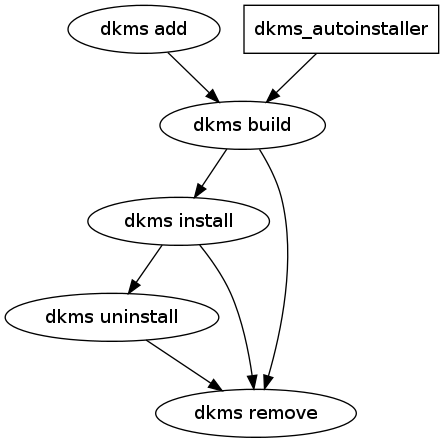
\includegraphics[width=0.4\hsize]{image201202/dkms.png}
 \end{center}
\label{fig:dkms}\caption{DKMS 全体の流れ}
\end{figure}

dkms\_autoinstaller はシステム起動時に呼ばれる
\footnote{ディストリビューションによって異なる}スクリプトです。
既に DKMS に登録(dkms add)されているドライバモジュールの中で、
現在起動しているカーネル用にドライバモジュールがインストール
(dkms install)されていないものがあれば、
ドライバモジュールのビルドとインストール
(dkms build / dkms install)が実行されます。

\subsubsection{モジュールソースコードの配置位置}

DKMS 対応モジュールのソースコードは
\url{/usr/src/ドライバモジュール名-バージョン/} 以下に配置する必要があります。
先のドライバの場合、\url{/usr/src/hello-0.0.1/} 以下に配置します。

\subsubsection{DKMS 設定ファイル}

DKMS は、各ドライバパッケージ毎に設定ファイルを持つ必要があります。
この設定ファイルでは、どのようなドライバが提供、ビルド、インストールされるのか
記述されている必要があります。以下によく利用する設定項目を示します。
\begin{table}[ht]
 \caption{DKMS 設定ファイル項目}
 \label{tab:dkms-config-file}
\begin{center}
  \begin{tabular}{|l|p{35zw}|}
 \hline
 設定項目 & 内容 \\
 \hline \hline
PACKAGE\_NAME & パッケージ名 \\
PACKAGE\_VERSION & パッケージバージョン \\
CLEAN & キャッシュなどの一時ファイルを削除するためのコマンドを指定する。
       指定しない場合には ``make clean '' が実行される。\\
MAKE & モジュールをビルドするコマンドを指定する。\\
BUILT\_MODULE\_NAME & ドライバモジュールの名前を指定する(拡張子は必要なし)。\\
BUILT\_MODULE\_LOCATION &  ビルドされたモジュールが作成されるディレクトリまでの相対パス\\
DEST\_MODULE\_LOCATION & モジュールをインストールするディレクトリを指定する。\\
AUTOINSTALL & モジュールを自動的にインストールするか、``yes'' か ``no'' を指定する。\\
REMAKE\_INITRD & ドライバインストール時に initrd イメージを再構成するか、``yes'' か ``no'' を指定する。 \\
PATCH & 適用したいパッチを指定する。\\
PATCH\_MATCH & パッチを適用するバージョンの指定する。Linux カーネルが 2.6.38 と 2.6.39 の場合にパッチを適用したい場合には ``\verb!2\.6\.(38|39)!'' と指定する。\\
 \hline
 \end{tabular}
\end{center}
\end{table}

BUILT\_MODULE\_LOCATION や BUILT\_MODULE\_NAME などは
配列を使ってドライバモジュール毎に設定できます。
BUILT\_MODULE\_NAME 配列の番号は各要素の番号に紐づいているので、
処理されるときは各々の番号が参照されます。
例えば、一つのドライバパッケージから foo と bar の2つのデバイスドライバ
が提供される場合、以下のように設定することができます。

\begin{commandline}
(省略)
BUILT_MODULE_NAME[0] = "foo"
BUILT_MODULE_LOCATION[0]  = "foo_build"
DEST_MODULE_LOCATION[0] = "/update"
BUILT_MODULE_NAME[1] = "bar"
BUILT_MODULE_LOCATION[1]  = "bar_build"
DEST_MODULE_LOCATION[1] = "/update"
(省略)
\end{commandline}

これにより、ドライバ foo のビルドは foo\_build ディレクトリで行われ、
update ディレクトリ以下にインストール、ドライバ bar のビルドは
bar\_build ディレクトリで行われ、update ディレクトリ以下にインストール
されます。

\subsubsection{DKMS で提供されるコマンド}
DKMS は dkms コマンドで操作します。
以下に利用頻度が高いコマンドを紹介します。

\begin{enumerate}
\item dkms status\\
DKMS で提供されている モジュールのステータスを表示します。
\begin{commandline}
$ dkms status
v4l2loopback, 0.5.0, 3.1.0-1-amd64, x86_64: installed
v4l2loopback, 0.5.0, 3.2.0-1-amd64, x86_64: installed
virtualbox, 4.1.8, 3.1.0-1-amd64, x86_64: installed
virtualbox, 4.1.8, 3.2.0-1-amd64, x86_64: installed
\end{commandline}
%$

\item dkms add \\
モジュールのソースコードを管理対象に追加します。
実行する時に -m オプションで追加するドライバパッケージ名を、
-v オプションでバージョンを指定します。

\begin{commandline}
$ sudo dkms add -m hello -v 0.0.1

Creating symlink /var/lib/dkms/hello/0.0.1/source ->
                 /usr/src/hello-0.0.1

DKMS: add completed.
$ dkms status
hello, 0.0.1: added
\end{commandline}
%$

実行すると/var/lib/dkms 以下に シンボリックリンクを張り、DKMS が管理する
ドライバデータベースに登録されます。

\item dkms build \\
管理対象になっているモジュールをビルドします。
実行する時に -m オプションで追加するドライバパッケージ名を、
-v オプションでバージョンを指定します。

ドライバは \url{/var/lib/dkms/ドライバ名/ドライババージョン/BUILT\_MODULE\_LOCATION} 以下
でビルドされます。
作成されたモジュールとビルドログは
\url{/var/lib/dkms/ドライバ名/ドライババージョン/カーネルバージョン/アーキテクチャ}
以下に置かれます。

\begin{commandline}
$ sudo dkms build -m hello -v 0.0.1

Kernel preparation unnecessary for this kernel.  Skipping...

Building module:
cleaning build area....
make KERNELRELEASE=3.0.0-1-amd64 -C /lib/modules/3.0.0-1-amd64/build M=/var/lib/dkms/hello/0.0.1/build....
cleaning build area....
\end{commandline}
% $

\item dkms install\\
dkms build コマンドによってビルドされたモジュールをdkms.conf の
DEST\_MODULE\_LOCATION で指定されている場所にインストールします。
例えば Linux カーネル 3.2.0-1-amd64 を使っていて、
\begin{commandline}
DEST_MODULE_LOCATION[0]="/updates"
\end{commandline}

と指定されている場合には \url{/lib/modules/3.2.0-1-amd64/updates/dkms/}
以下にインストールされます。

\begin{commandline}
$ sudo dkms install -m hello -v 0.0.1

hello:
Running module version sanity check.
 - Original module
   - No original module exists within this kernel
 - Installation
   - Installing to /lib/modules/3.0.0-1-amd64/updates/dkms/

depmod..........

DKMS: install completed.
$ dkms status
hello, 0.0.1: installed
$ sudo modprobe -l | grep hello.ko
updates/dkms/hello.ko
\end{commandline}
%$

\item dkms uninstall\\
モジュールをアンインストールします。
実行する時に -m オプションで追加するドライバパッケージ名を、
-v オプションでバージョンを指定します。
また全てのカーネルから削除する場合には --all オプション、
特定のカーネルモジュールのみを削除する場合には -k オプションでカーネル
バージョンを指定します。

\begin{commandline}
$ sudo dkms uninstall -m hello -v 0.0.1 -k 3.0.0-1-amd64

-------- Uninstall Beginning --------
Module:  hello
Version: 0.0.1
Kernel:  3.0.0-1-amd64 (x86_64)
-------------------------------------
(中略)

depmod....

DKMS: uninstall completed.
\end{commandline}
%$

% 中略部分
\if 0

Status: Before uninstall, this module version was ACTIVE on this kernel.

hello.ko:
 - Uninstallation
   - Deleting from: /lib/modules/3.0.0-1-amd64/updates/dkms/
 - Original module
   - No original module was found for this module on this kernel.
   - Use the dkms install command to reinstall any previous module version.

\fi

\footnote{この資料を作成している時点では、「dkms uninstall」は動作しません。
一部のチェックが未実装なため、uninstall の処理まで行われないためです。
\url{http://bugs.debian.org/cgi-bin/bugreport.cgi?bug=659672}}

\item dkms remove\\
DKMS の管理対象から外します。uninstall と同様のオプションが必要です。
ドライバモジュールがアンインストールされていない場合、アンインストールを実行してから、
管理対象から外れるようになっています。

\begin{commandline}
$ dkms status
hello, 0.0.1, 3.0.0-1-amd64, x86_64: installed
virtualbox, 4.1.6, 3.0.0-1-amd64, x86_64: installed
$ sudo dkms remove  -m hello -v 0.0.1 --all

-------- Uninstall Beginning --------
Module:  hello
Version: 0.0.1
Kernel:  3.0.0-1-amd64 (x86_64)
-------------------------------------
(中略)

depmod....

DKMS: uninstall completed.

------------------------------
Deleting module version: 0.0.1
completely from the DKMS tree.
------------------------------
Done.
$ dkms status
\end{commandline}
%$

% 中略部分
\if 0

Status: Before uninstall, this module version was ACTIVE on this kernel.

hello.ko:
 - Uninstallation
   - Deleting from: /lib/modules/3.0.0-1-amd64/updates/dkms/
 - Original module
   - No original module was found for this module on this kernel.
   - Use the dkms install command to reinstall any previous module version.


\fi

\end{enumerate}

その他、rpm パッケージを作成する mkrpm オプションや Debianパッケージ
を作成する mkdeb オプションなどが用意されています。

\subsection{DKMS 対応Debian パッケージの作り方}

上記での説明のように、DKMS 対応モジュールのソースを規定のディレクトリに
展開しておくと DKMS は処理を行います。Debian の場合もパッケージ化するときは
インストールした時に規定のディレクトリに展開するようにしておきます。
パッケージ名などに関してはルールが決まっており、 DKMS 対応パッケージは
-dkms というサフィックスがついています。
これはパッケージ名がわかりやすいという理由と、DKMS 用の debhelper
コマンド、dh\_dkms コマンドが -dkms サフィックスのついたパッケージに
対して処理を行うためです。
debian/パッケージ名.dkms または debian/dkms を dkms.conf に変換して、
適切な dkms 用ディレクトリにコピーし、postinst と prerm に DKMS 用の
処理を追加します。
dh\_dkms コマンドは dkms パッケージで提供されています。
debhelper 7 以降で利用する場合には、アドオンとして読み込ませる必要
があります。

debian/hello-dkms.dkms:
\begin{commandline}
PACKAGE_NAME="hello"
PACKAGE_VERSION="#MODULE_VERSION#"
BUILT_MODULE_NAME[0]="$PACKAGE_NAME"
BUILT_MODULE_LOCATION="src"
DEST_MODULE_LOCATION[0]="/updates"
AUTOINSTALL="yes"
\end{commandline}
%$

DKMS 用 debian/rules:
\begin{commandline}
#!/usr/bin/make -f

VERSION := $(shell dpkg-parsechangelog | sed -nr '/^Version:/s/Version: (.*:)?(.*)-(.*)/\2/p')

%:
    dh $@ --with dkms
override_dh_install:
    dh_install src/* usr/src/hello-$(VERSION)/src/
    dh_install Makefile usr/src/hello-$(VERSION)/
override_dh_dkms:
    dh_dkms -V $(VERSION)

override_dh_auto_configure override_dh_auto_build override_dh_auto_test override_dh_auto_install override_dh_auto_clean:
\end{commandline}
%$

debian/rules ファイル内で override\_dh\_auto\_configure や
override\_dh\_auto\_build を呼び出している理由は Makefile がある場合、
make が実行されてしまうのでこれを抑制するためです。

\subsubsection{Debian でのドライバモジュールビルドのタイミング}

Debian では DKMS ドライバパッケージがインストールされた後と、
カーネルヘッダ または カーネルイメージパッケージがインストール
(更新)された後、 dkms が起動してドライバモジュールのコンパイルが行われるよ
うになっています。これらは以下のファイルで処理されます。

\begin{commandline}
/etc/kernel/postinst.d/dkms
/etc/kernel/header_postinst.d/dkms
\end{commandline}

\subsubsection{Debian の DKMS 対応状況}

主要なドライバの殆どは DKMS と module-assistant(以下 m-a)の両方
に対応しています。開発があまり活発ではないドライバは m-a のみ
をサポートした状態が多いようです。
新しくパッケージ化されたドライバはほとんどが両方に対応しています。
DKMS のほうがメリットが多いため、m-a から DKMS に切り替えているユーザ
も多いようです。

\subsection{module-assistant との違い}
Debian には他のドライバパッケージ管理機構に
module-assistant(m-a)があります。
DKMS と m-a の違いには以下のようになっています。
\begin{itemize}
\item m-a は自動ビルド機構がない。\\
カーネルが更新されると、手動で m-a を実行する必要があります。
\item DKMS はドライバ用のバイナリパッケージを作らない。\\
m-a は カーネル毎バイナリパッケージを作り、それをインストールします。
\item m-a は起動しているカーネルのみのドライバをビルドするが、DKMS は
インストールされているカーネルをビルドできる。
\end{itemize}

\subsection{まとめ}

今回は DKMS の基本的な仕組みと、Debian での DKMS 対応パッケージ作成方法
について説明しました。今までは m-a が主流だったのですが DKMS もサポート
しているドライバパッケージも増え始め、徐々に DKMS に移行しつつあるように
感じました。Debianパッケージ用ツールが用意されているため、
対応パッケージ作成も難しくないと思います。
今後ドライバパッケージを作成する場合には、DKMS をサポートしてみては
いかがでしょうか。

\clearpage

%-------------------------------------------------------------------------------
\dancersection{さきが(ry NM 塾}{倉敷悟}
%-------------------------------------------------------------------------------
\index{NM}
\index{New Member}

\subsection{NM とは何か}

Debian における NM (New Member) とは、新しく Debian Project の参加メンバーになった人、あるいは Debian Project
に参加するための手続き、といった意味で使われます。後者の場合は、意味を明確にするために、NM プロセスといったりもします。
少し前までは、New Maintainer の略だったのですが、(パッケージ) メンテナ以外にも門戸を開こう、という方向性に変更されつつあります
(とはいえ、現時点では NM プロセスはまだパッケージメンテナを念頭においた形のままです)。

\subsection{NMプロセスの紹介}

では、実際のNMプロセスを実例をもとにご紹介します。本当はもう少しプロセスを進めておくつもりだったのですが、あまりスムーズにいってないので途中までになっています。

NM 志願者向けのチェックリスト (http://www.debian.org/devel/join/nm-checklist) がありますので、まずはこれを見てみましょう。

\subsubsection{必要な条件}

まず、Debian Developer(以下DD) 2 名以上とキーサインしていること、さらに NM への応募を推薦してくれる DD が 1 名以上いること、
これは具体的かつ最低限の条件になります。
加えて、すでに Debian に関わるある程度の活動をしてきていることも必要とされますが、これについては明確な線引きがあるわけではありませんし、今後変化してくる部分なので水物といっていいでしょう。

私の例だと、まともに Debian での活動をはじめたのは 2007 年くらいだったと思うので、おおよそ 4 年間、下積みとしてパッケージメンテ、翻訳、ローカルコミュニティ活動をしてきていますが、これはちょっと長かった (NM 応募が遅かった) かなぁ、と思っています。

最近では、DM のステップをふんでいることが推奨されていることもあるので、少なくとも6ヶ月以上特定のパッケージをメンテしていて、スポンサーと良好な関係を築けていれば、そのまま NM に進むことも可能でしょう。

\subsubsection{実例}

\begin{itemize}
\item 2011/11 (事前ネゴ)
\item 2011/12/04 apply
\item 2011/12/04 advocate checked by yyabuki
\item 2011/12/10 activity poll sent
\item 2011/12/11 pass frontdesk precheck
\item 2011/12/13 AM assigned to gwolf
\item 2011/12/16 AM assigned to laney
\item 2011/12/17 ID checked
\item 2011/12/25 (Philosophy and Procedure やりとり中)
\end{itemize}

この後に続く予定は、次のようになっています。

\begin{itemize}
\item Tasks and Skills
\item AM recommends to DAM
\item DAM Approval
\end{itemize}

\subsubsection{NMテンプレート}

NM 担当チームでは、主に AM 担当者向けの資料として、作業ガイドのリポジトリが用意しています(\url{http://anonscm.debian.org/viewvc/nm/trunk/nm-templates/})。実は、ここを見れば、だいたい何を聞かれるのかはわかってしまいますので、予習のための参考書としては最良のものだと思われます。ただし、AM によっては NM テンプレートを使わない、という人もいますので、盲信はしすぎないようにしましょう。

\subsubsection{NM と 勉強会と Debian JP}

Debian 勉強会では、Debian Developer を育成する、を目的としてあげています。ですので、その運営主体である Debian JP としても、支援活動はいろいろとおこなわれています。具体的には、GPG キーサインの推進や、スポンサー探しのサポート、パッケージングスキルの教育、などです。是非有効に活用してください。

\subsubsection{NM と Debian Maintainer}

勉強会でも何度かとりあげていますが、いきなり NM は敷居が高い、という人のために、DM というステップが用意されています。これは、いわば「限定つきの Debian Developer」であり、スポンサーについてもらうことで自分のパッケージを Debian に含めることができる人達のことです。

事前の実績としてわかりやすいことや、内容がサブセットになっていることもあり、NM プロセスにおいても、事前に DM として活動しておくことが強く推奨されています。

\subsection{最後に}

\subsubsection{なぜ NM に?}

NM になることの意義を考えてみましょう。直接的には、次のようなメリットがあります。

\begin{itemize}
\item パッケージを自由にアップロードできる
\item LWN.net の購読権 (sponsored by HP)
\item Project Leader や GR への投票
\item @debian.org メールアカウント
\end{itemize}

あるいは若い人であれば、比較的名前の知られたプロジェクトへの参加自体や、プロジェクトに自分色を持ち込める、といった満足もあるかもしれません。
ただ、NM プロセスやその後の活動は、それなりに手間も気力も必要になります。これじゃ引きが足りない、という人も多いでしょう。

Debian 勉強会としては、前述したとおり、NM に応募しようと思える人材を育成したい、という思いがあるのですが、やはり動機の部分については、皆さんそれぞれの答えを見出していただくしかありません。

スライドの方では、一例として、特に技術的に秀でたものをもっているわけでもなく、業界的には定年に達してしまったおっさんが、一体何を考えて NM に挑戦してみているのか、簡単に紹介してみます。参考になれば。

\clearpage

%% -*-tex-*-
%%
%% Copyright (C) 2012 Hiroshi Kubo  all rights reserved.
%% 本資料の著作権は、著者である久保博 <h-kubo@geisya.or.jp> にあります。
%%
%% This document material is licensed under the GNU General Public License version 2.0.
%% This document is originally in the form of LaTeX source code. This shall be referenced as the ``Corresponding Source''
%% Any compiled forms including DVI, Postscript, and PDF from the original source code shall be reference as the ``Object code''.
%%

%-------------------------------------------------------------------------------
\dancersection{フリーソフトウェアと戯れるための著作権入門}{山城国の住人 久保博}
%-------------------------------------------------------------------------------
\index{Free software}
\index{ちょさくけん@著作権}

\subsection{前書き}

人生のいきがかり上、割と最近になって著作権の勉強を始めることになりました。
法律の専門家ではありませんので、自信を持っての発表ではないですが、
みなさんと一緒に考えていくきっかけになればと思います。

\subsection{はじめに}

日本を含む多くの国で、ソフトウェアは、生み出された時から著作権という権利の対象になっています。

ですから、フリーソフトウェアも、生まれた時から誰かのもの、ということになっています。
フリーであっても誰かのものである、という点では、登記された土地は空き地であっても誰かのものであるのとにているかも知れません。

フリーソフトウェアの精神は、一介の利用者が自分自身のためにソフトウェアを使うことを
妨げるようなことは最大限避けるようにしていますから、自分自身のためにフリーソフトウェアを使う限り、
知らなくても困ったことにはなりません。

でも、そこから一歩踏み出そうとすれば、誰かのものであるということを尊重することが求められることになります。
この要請は、著作権法と、それを前提とする契約に基づいています。

そこで、Debian Project が配布しているようなフリーソフトウェアを扱う場面をいくつか想定して、
そこに著作権と契約がどのように関わってくるのか、解き明かしてみます。なお、日本の著作権法を元にしてお話します。



\subsection{知的財産権}

ソフトウェアが誰かのものである、とは、どういうことでしょう。

知的な作業を通して創り出された、無体物(プログラムを含む)には、
創り出した人の努力や労力に報いるために、さまざまな制度を定める法律が整備されています。
その中でも、知的な創造によってつくり出された無体物に対して、
財産権の対象となる有体物の物権に良く似た権利を設定する仕組みが法律で定められています。
この物権に似た権利を知的財産権といいます。
そして、知的財産権は、創造した人あるいは登録した人が享受する権利なのです。

これが、ソフトウェアが誰かのものである、ということの、現代社会における意味です。

ソフトウェアが関係する知的財産権には、次のものがあります。

\begin{itemize}
\item[{\bf{著作権}}] 「思想又は感情を創作的に表現したものであつて、文芸、学術、美術又は音楽の範囲に属するもの」に対する独占的な保護をもたらす権利
\item[{\bf{特許権}}]  発明(自然法則を利用した技術的思想の創作のうち、高度なもの)を登録することによって独占的な保護をもたらす権利
\item[{\bf{実用新案権}}] 考案(自然法則を利用した技術的思想の創作)を登録することによって独占的な保護をもたらす権利
\item[{\bf{意匠権}}] 意匠(物品の形状、模様若しくは色彩またはこれらの結合であって、視覚を通じて美感を起こさせるもの)を登録することによって独占的な保護をもたらす権利
\item[{\bf{商標権}}] 商標を登録することによって独占的な保護をもたらす権利
\end{itemize}

プログラムそのものは、著作権の対象になります。
また、プログラムで実装されたアルゴリズムは特許や実用新案の保護の対象になり得る場合がありますし、プログラムの名称やロゴは商標としての保護の対象になり得ます\footnote{Debian も電子計算機などの指定商品での商標登録がされており、登録番号は 第4595288号です。ちなみに、指定商品「菓子、パン」で「デビアン」という称呼の登録番号第1708032号の登録商標があります。面白いですね。}。
GUIの画面のデザインは海外では意匠登録の対象となり得る場合もあるようですが、日本では今のところ対象ではありません。

この中でも、ソフトウェアについて一番よく問題になるのは、著作権です。

\subsection{著作権}
\subsubsection{著作権の性質}

正確ではないですが端的に言えば、著作権法は、著作物を作った人に著作物に対する独占的な権利を与える法律です。
その著作権法で定められている著作権には次のような性質があります。

\begin{itemize}
\item 著作物を作ったら、発生します。
\item 著作物を公表しなくても発生します。
\item (特許と違って、)役所に登録しなくても発生します\footnote{このような権利の発生のさせ方を無方式主義と言います。なお、かつてアメリカは、無方式主義ではありませんでした。}。
\item 著作物が生まれてから、著作者の死後50年間、著作権の保護は続きます。
\item 他人が著作物を勝手に利用した場合、差止請求権、損害賠償請求権を行使するという方法で対抗できます\footnote{著作権法第百十四条に基づいて損害額を推定しても、フリーソフトウェアの場合、0円にしかならないですが…。}。
\end{itemize}
ですから、新しいプログラムが作られれば、必ずと言っていいほど著作権が関係してきます。

逆に言えば、著作物をパブリックドメインとするためには、著作権を放棄する手続きなどが必要になるわけです。
また、著作物を利用するには、著作権者から利用許諾をもらうべし、というのが著作権法に則った正しい方法です。

したがって、ソフトウェアとともに
\begin{itemize}
\item 著作権に基づく利用許諾契約書
\item 著作権を放棄する宣言あるいは放棄済であることの明示的な説明
\end{itemize}
のどちらかを手に入れないと、著作権法に違反していない確信を持ってソフトウェアを使うことが難しい、ということになります。
Debian Project は、社会契約\cite{DebianSocialContract}に基づいて行動しており、この点に関して厳密に考えてパッケージを作っているわけです。

\subsubsection{著作権の存続期間}

権利が有効である時間の範囲を存続期間と言います。

「著作者が死んでも著作権の保護が続くってどういうこと?」と不思議に思うかも知れませんね。
 著作権は相続できるのです。相続する人があれば、続くんです。
相続を含めて、権利を引き継ぐことを「承継」と言います。
承継する人がなければ、著作権は消滅します。

\par
\begin{center}
\fbox{
\parbox{0.8\linewidth}{
\begin{center}{\Large\bf 筆者からお願い!}\\
あなたが作って公開しているプログラム、\linebreak[1]あなたの死後に誰が著作権を相続するか予め周りの人に教えておいて下さい。
\end{center}
}
}
\end{center}
\par


なお、FSF\footnote{Free Sofware Foundation. ウェブサイトは {\url http://www.fsf.org/}}は、FSFへ著作権を譲渡することを勧めています\cite{FSFassign}。著作者の死後、GPL\footnote{GNU General Public License}で公開したフリーソフトウェアの行く末を託すこともできますね\footnote{著作権の譲渡に関しては、日本の著作権法には第三者対抗要件に登録が必要などの難しい話が関係するので、筆者はどうしたらいいのか、理解できていません。}。

\subsubsection{著作権の内訳}

著作権とは、権利の束みたいなものです。著作物を利用する方法などによって、細かい権利が定められています。

それらは大別すると、「著作人格権」と「著作財産権」に分かれ、それぞれの下に次のような権利が条文で定められています。

\begin{description}
\item[著作人格権]「公表権」「氏名表示権」「同一性保持権」
\item[著作権(著作財産権)]「複製権」「上演権」「演奏権」「上映権」「公衆送信権」「伝達権」「口述権」「展示権」「頒布権」「譲渡権」「貸与権」「翻訳権」「翻案権」「二次的著作物の利用に関する権利 」
\end{description}

この中には、ソフトウェアが関係しないものもあります。

\subsection{Debian Project が配布しているものの何が著作物?}

さて、著作物とはどんなものがあるか、著作権法を読んでみると、次のようなことが書いてあります。

著作物とは、「思想又は感情を創作的に表現したものであつて、文芸、学術、美術又は音楽の範囲に属するものをいう。」
(著作権法第二条)


更に、著作権法では、例を挙げて著作物を定義しています。

\begin{verbatim}
第十条 この法律にいう著作物を例示すると、おおむね次のとおりである。
  	一 小説、脚本、論文、講演その他の言語の著作物
  	二 音楽の著作物
  	三 舞踊又は無言劇の著作物
  	四 絵画、版画、彫刻その他の美術の著作物
  	五 建築の著作物
  	六 地図又は学術的な性質を有する図面、図表、模型その他の図形の著作物
  	七 映画の著作物
  	八 写真の著作物
  	九 プログラムの著作物

2 事実の伝達にすぎない雑報及び時事の報道は、前項第一号に掲げる著作物に該当しない。

3 第一項第九号に掲げる著作物に対するこの法律による保護は、その著作物を作成するために用いるプログラム言語、規約及び解法に及ばない。この場合において、これらの用語の意義は、次の各号に定めるところによる。
  	一 プログラム言語 プログラムを表現する手段としての文字その他の記号及びその体系をいう。
  	二 規約 特定のプログラムにおける前号のプログラム言語の用法についての特別の約束をいう。
  	三 解法 プログラムにおける電子計算機に対する指令の組合せの方法をいう。
\end{verbatim}

ということで、プログラムは、プログラム著作物です。オブジェクトコードもプログラム著作物である、という判例もあるようです\footnote{東京地判昭和60年3月8日判タ 561号 169頁「ディグダグ」事件 という判例があるそうです\cite{saito}。}。

また、Debian Project が配布するものにはプログラム以外にも、文章、写真画像、地図データなどありますが、著作物です。


\subsection{著作権を踏まえた Debian Project からの配布物とのおつき合い}


\subsubsection{著作権のことを気にせずに Debian のシステムをインストールしました。何かまずいことをしていないでしょうか?}

自分で使う目的でインストールしたのですよね?

インストールする前に利用許諾契約を読んで、同意して、それからインストールするのが理想的ですが、そうでない場合もよくあるかと思います。

Debian Project が配っているインストーラーを使って普通にインストールしたなら、
インストールしたソフトウェアの利用許諾契約に同意したことにしましょう。
インストーラーでインストールしたソフトウェアはすべて DFSG\footnote{The Debian Free Software Guidelines\cite{DFSG}} に準拠しているので、ほとんどあなたは不利益を被っていません。

\begin{itemize}
\item 金銭的な対価は要求されません。
\item 使うだけなら無償の貢献も要求されません。
\item あなたの某かの権利を放棄したり断念したり譲渡したりすることもありません。
\end{itemize}

なにか気をつけることがあるとすれば、免責条項くらいでしょうか。

 ほぼすべてのフリーソフトウェアの利用許諾では、その動作に関して無保証で、免責条項が盛り込まれています\footnote{フリーでなくても、無保証である場合が多いですし、保証はあっても賠償額の上限をソフトウェア購入代金とすることも珍しくありません。}。
無保証であることに関する同意は、ほとんどのソフトウェアが採用している利用許諾の契約の条項の一部です。同意できないなら、利用する権利はありません。

したがって、著作者に対して、次に掲げることについて何の文句をつける筋合いもありません。
\begin{itemize}
\item  期待通りに動かない
\item  そもそも動かない
\item  ソフトウェアを使ったせいで、地位や財産を失った
\item  ソフトウェアを信じたせいで、地位や財産を失った
%%\item  ソフトウェアを使ったせいで、心が傷ついた
\end{itemize}

%% ここで BTS の話を一席
でも、多くのフリーソフトウェアの開発元や Debian Project には、バグ報告の窓口がありますね。
あれは、義務でやっているのでないのです。大いなる親切以外の何物でもありません。


%% \subsubsection{知合いのパソコンに Debian のシステムをインストールしました。}

%% そのパソコンを利用する持ち主の方に、利用許諾書に同意してもらいましょう。
%% 別に、書類に判子をつくような手続きは必要ありません。

%% 全部を理解してもらうのはなかなか困難だとは思いますが、
%% 自分のために使って、うまくいかなくても作者の方々に文句をいう筋合いはないことに納得してもらえれば実際上は十分です。


\subsubsection{Debian のフリーソフトウェアを使わないけど配ります。}

ちょっと待って! あなたは、著作者と契約を結ばなくてはなりません!

著作権には「複製権」「自動公衆送信権」「送信可能化権」という権利が含まれているのです。
極めて簡単に分かりやすくいうと
\begin{description}
\item[複製権 ] 簡単にいうと、コピーする権利。
\item[自動公衆送信権] 公衆に送信する権利。
\item[送信可能化権] 公衆がアクセスしてダウンロードできるサーバーに著作物を置く権利。
\end{description}
です。
著作者が独占的に保持する権利ですから、あなたは、ソフトウェアを配ったり、公開されているサイトにアップロードする前には、著作者の許可が必要です。


でも実は、Debian アーカイブの main セクションと contrib セクションに含まれるソフトウェアのソースコードを
{\em そのまま}無料で配布する場合は、利用許諾に同意する必要はあるものの、
実質的には何らかの義務や制約に縛られることはありませんので、
ほとんど気にかける必要はないです。

というのも、main と contrib に含まれるソフトウェアは、すべて DFSG\cite{DFSG} に準拠してます。
DFSG に準拠しているこということは、ソースコードの自由な配布が利用許諾契約上、認められていることになるのです。

これに対して、バイナリパッケージを配布する場合は、配布先でソースコードが手に入れることができるように配慮しないといけないライセンスが多いです\footnote{GPL や LGPL (GNU Lesser General Public License)  が典型的な例です。}。
ソースコードが入手できるような配布を強制することで、ソフトウェアの自由を担保しようとしているわけです。
注意しましょう。


また、利用許諾の内容を理解する前に、適当に一部を削ったり、一部を抜き出して配らないようにしましょう。
というのも、著作権には「同一性保持権」という権利があります。
勝手に削ることも含めて、著作物を勝手に改変することは著作権法が禁じています。
改変に際しては許諾が必要で、許諾された範囲での改変しか許されません。

幸い、 DFSG準拠なら改変は許されますし、改変されたソフトウェアの複製を配布することも許されますが、
契約毎に許されるための条件はあります。

それから、勝手に著作者の氏名を削ってはいけません。
「氏名表示権」を侵害することになります。

\par\begin{center}{\Large そのまま配るのが一番無難です。}\end{center}

\subsubsection{Debian をインストールされてるパソコンをもらいました}

一般的に、正規の方法で入手したソフトウェアを手元にコピーを残さずに誰かに譲り渡すことは構わないのですが、
パソコンをもらっただけでは、そのパソコンにインストールされているソフトウェアを無条件に使っていいことにはなりません。
くれた人は「好きにしていいよ」と言ってくれていても、利用許諾の契約には同意して利用しましょう。

物品の譲渡と一緒に著作権の利用許諾がなされたとみなせる場合というのは、
特別に著作権法に明記されています\footnote{美術品の展示権など。}。
原則として、物品の譲渡とそこに宿っている著作物の利用許諾とは、別ものなのです。

ちなみに、ソフトウェアの利用許諾書にはしばしば non-transferable という言葉で、
利用権の譲渡を明示的に禁止する文言が現れますが、その場合は、契約上利用権を譲渡できないことになっています。

\subsection{特許との関係}

利用許諾書には、著作権ではない別の知的財産権に基づく利用許諾が含まれる場合があります。
よく使われる「ライセンス」と言う言葉に含まれる、利用許諾の根拠になる権利は著作権だけとは限らないわけです。

例えば、DFSG準拠の利用許諾の中には、特許に関する条項が含まれているものがあり、
その代表的なものには、 Apache License 2.0 と、 GPL 3.0 があります。

この二つの利用許諾には、ともに、「ソースコードの貢献者が保有する特許のうち、ある範囲のものは、無償で利用を許諾する、」という趣旨の条項が含まれています。
Apache License 2.0 は、貢献者が自分の貢献したコードに含まれる特許を利用許諾するのに対し、
 GPL 3.0 では、貢献者が配布したコードに含まれる特許を利用許諾する点が違います。


\subsection{その他関係する法律}

最後に、ソフトウェアが関係しそうな法律をいくつか挙げておきます。

\begin{itemize}
\item 不正アクセス禁止法
\item 不正競争防止法
\item 刑法のいわゆるウィルス作成罪
\item 関税法
\item 民法
%% \item PL法
\end{itemize}


\subsection{宿題}

次の問題に答えてみましょう。

\begin{itemize}
\item 「アルゴリズム体操」の振付けは、著作権法第十条の何の著作物でしょうか?
\item GCC (GNU Compiler Collection) は、プログラムの著作物として保護されるでしょうか?
\item 著作権(著作財産権)のうち、ソフトウェアに関係あるものを挙げてみましょう。
\item かつて特許によって自由な配布が制限されたソフトウェアがありました。どんなものがあるか、調べてみましょう。
\end{itemize}



\subsection{まとめ}


フリーソフトウェアに関わる著作権の仕組みを簡単に解説しました。

\begin{thebibliography}{99}
    \bibitem{DebianSocialContract} Debian 社会契約,
                    \url{http://www.debian.org/social\_contract}

    \bibitem{DFSG} The Debian Free Software Guidelines,
    \url{http://www.debian.org/social\_contract\#guidelines}

    \bibitem{CopyrightLaw} 著作権法 ,
                    \url{http://law.e-gov.go.jp/htmldata/S45/S45HO048.html}

    \bibitem{FSFassign} なぜFSFは貢献者に著作権の譲渡をお願いしているのか {\url http://www.gnu.org/licenses/why-assign.html}

    \bibitem{GPLv3chikujou} GPLv3 逐条解説
      \url{http://ossipedia.ipa.go.jp/DL/doc/187/5/0904/ON/}

    \bibitem{saito} 著作権法 , 斉藤博, 2000年, 有斐閣

\end{thebibliography}

\clearpage
%-------------------------------------------------------------------------------
\dancersection{ITP から始めるパッケージメンテナへの道}{よしだ ともひろ}
%-------------------------------------------------------------------------------
\index{ITP}
\index{Package Maintainer}
\index{ぱっけーじめんてな@パッケージメンテナ}

\subsection{はじめに}
とある便利なソフトウェアを見つけて、それがまだDebianパッケージになっていなかった
とき、RFP(Request For Package:パッケージ化の要求)をしてもよいのですが、自分でパッ
ケージ化してDebianの一部として提供することもできます。そこで、ITP(Intent To Package:
パッケージ化の宣言)からアップロードまでの流れをまとめてみました。

\subsection{まずはITP}
\subsubsection{ITPの前に必要なこと}
\subsubsubsection{既にパッケージ化されていないか?}
\url{http://www.debian.org/distrib/packages}で探してみたり、aptitude searchや
apt-cache searchで確認してみましょう。

\subsubsubsection{既にITPされていないか?}
他の誰かが同じようにパッケージ化しようと思って、ITPしているかもしれません。

\url{http://www.debian.org/devel/wnpp/being\_packaged}をチェックしてみましょう。

\subsubsubsection{既にRFPされていないか?}
他の誰かが、パッケージ化して欲しいと思って、RFPしているかもしれません。
RFPされている場合は、ITPすることでパッケージ化の宣言を行います。

\url{http://www.debian.org/devel/wnpp/requested}をチェックしてみましょう。

\subsection{ITPの仕方}
パッケージをITPするのはreportbug(apt-get|aptitude install reportbug)で行う方法が
\url{http://www.debian.org/devel/wnpp/}で紹介されています。また、電子メールでも
行うことができます。ここでは、電子メールでITPを行う方法の一つ、Mewを使う方法を
紹介します。

まず、debian-elパッケージをインストールします。

\begin{commandline}
   $ sudo aptitude install debian-el
\end{commandline}
%$ for emacs font-lock

次に\texttt{\~{}/.emacs}に以下を追加します。

\begin{commandline}
(autoload 'mew "mew" nil t)
(autoload 'mew-send "mew" nil t)

(if (boundp 'read-mail-command)
	(setq read-mail-command 'mew))
(autoload 'mew-user-agent-compose "mew" nil t)
(if (boundp 'mail-user-agent)
	(setq mail-user-agent 'mew-user-agent))
(if (fboundp 'define-mail-user-agent)
	(define-mail-user-agent
		'mew-user-agent
		'mew-user-agent-compose
		'mew-draft-send-message
		'mew-draft-kill
		'mew-send-hook))
\end{commandline}

こうしておいてemacsを起動し、\texttt{M-x debian-bug RET}とします。
ミニバッファに

\begin{commandline}
Report a bug for a [P]ackage or [F]ile: (default P)
\end{commandline}

と表示されるので``P''を入力します。
パッケージ名を聞いてきますのでwnppと入力します。wnppというのはWork-Needing and
Prospective Packages(作業が望まれるパッケージ)という擬似パッケージのことで、ITP
やRFPを行うときに使用する他、RFH(Request For Help:助力の要求)、RFA(Request For
Adoption:養子引き取りの要求)、O(Orphan:みなしご)、ITA(Intent To Adopt:養子引き
取りの表明)にも使います。

次にActionを聞かれます。TABを押すと候補が表示されますのでITPとします。

あとは、パッケージ名、パッケージの簡単な説明を入力します。debian-develへCCするか?
も聞かれますので ``y'' と入力するとメールの雛形が表示されますので、残りのVersion、
Upstream Author、URL or Web page、Licenseを入力してメールを送信します。

\subsection{GnuPGキーサイン}
Debian公式パッケージにするにはdscファイルとchangesファイルに署名が必要です。
GnuPG(GPG)で署名しますが、信頼された鍵でないと意味がないのでキーサインパーティな
どでDebian開発者の方とキーサインをしておきましょう。GPG公開鍵は後に説明する
mentors.debian.netを使う時にも必要ですので、まだ、作成していない方は作っておくこ
とをおすすめします。

2012年6月23日(土)の大統一Debian勉強会でもキーサインパーティが予定されていますので、
是非参加しましょう。

\subsection{パッケージ作成}
パッケージの作成方法は過去のDebian勉強会などでも何度か紹介されていますので、
ここでは詳細は割愛し注意する箇所のみとします。

\subsubsection{lintian cleanにする}
lintianはDebianパッケージを精査し、バグやポリシー違反を報告します。アップロードす
る前に、必ずそのパッケージに対してlintianを実行してください。lintianを実行する際
はオプションの -v を付けてchangesファイルを指定します。lintianが出力する情報がわ
かりにくければ -i オプションを追加しましょう。出力される情報に ``E:'' や
``W:'' がなく
なるように修正し、lintian cleanにしましょう。

\subsubsection{パッケージに署名する}
お試しでパッケージを作ったりする場合はパッケージへの署名を省略しますが、公式パッ
ケージにするにはちゃんと署名することが必要です。debuildやdpkg-buildpackageで-us -uc
オプションをつけずにパッケージ作成すると、dscファイルとchangesファイルにGnuPGで署
名すためのパスフレーズを聞いてきますので入力すればOKです。

\subsection{mentors.debian.netへ登録}
\subsubsection{mentors.debian.netとは}
Debianへのパッケージアップロード権限はDebian開発者のみが持っているのですが、Debian
開発者でない人もアップーロードできる仕組みがあります。Debian開発者の方にスポンサー
になっていただいて、助言をいただきながら修正していく場、といった感じです。

\subsubsection{サインアップ}
\url{http://mentors.debian.net/}に ``Sign me up'' という
\url{http://mentors.debian.net/register/register}へのリンクがありますのでクリック
します。

Full name, E-mail, Password, Confirm passwordを入力し、Account typeはMaintainerを
選択してSubmitを押下します。入力したE-mail Addressへ確認のメールが飛んできますの
で、記載されたURLへアクセスしてActivateするとアカウントが使用可能になります。

ログインして、My accountページのChange GPG keyでGPGキーを登録できますのでアスキー
形式でエクスポートした公開鍵のファイルを選択して登録しておきます。

\subsubsection{アップロード}
mentors.debian.netにアップロードする方法は、duploadやdputなどのツールで行えます。
今回はdputで行う方法をご紹介します。

\begin{enumerate}
\item 準備

\texttt{\~{}/.dput.cf}を作ります。内容は\url{http://mentors.debian.net/intro-maintainers}を
参考にしました。httpとftpの設定が記載されているのですが、httpの設定としました。
こんな感じです。

\begin{commandline}
[mentors]
fqdn = mentors.debian.net
incoming = /upload
method = http
allow_unsigned_uploads = 0
progress_indicator = 2
# Allow uploads for UNRELEASED packages
allowed_distributions = .*
\end{commandline}

\item さあ、アップロード

いよいよアップロードです。\texttt{dput mentors \textit{changesファイル}} で行います。ここまでのパッ
ケージ作成で問題がなければmentors.debian.netへのアップロードは成功するはずです。

しばらくするとmentors.debian.netからメールが飛んできます。メールの内容は「スポン
サーが必要ならスポンサーを探してるにしろ」とか、「RFS(request for sponsorship)で
スポンサーを募集できるよ」というような内容ですので従います。
\end{enumerate}

\subsection{スポンサーを探す}
無事 mentors.debian.net へアップロードできたら debian-mentors@lists.debian.org や\\
debian-devel@debian.or.jp にRFS(request for sponsorship)を投げて、スポンサーになっ
てくれる方を探します。

\subsection{おわりに}
今回、はじめてITPして、mentors.debian.netにアップロードしてみました。色々調べたり
しながらでしたので時間はかかりましたが、それほど難しくはないと思います。Debianパッ
ケージになっていないソフトウェアを見つけたら是非ITPしましょう!

%-------------------------------------------------------------------------------
\dancersection{t-code のバグレポートをしてみた}{西田孝三}
%-------------------------------------------------------------------------------
\index{t-code}
\index{ばぐれぽーと@バグレポート}

\subsection{はじめに}

ここでは「Debianパッケージのバグを発見した場合にどうすればいいのか」を伝えることを目的とし、
実際のバグ例を挙げながらバグレポートの手順を説明します。
バグレポートするパッケージはEmacsで日本語入力するための拡張Elispであるt-codeパッケージです。
手順の大きな流れは下記の4段階に分けられます。

\begin{enumerate}
  \item バグトラッカーでの報告
  \item 自分で修正パッチを作る(可能であれば)
  \item 自分でDebianパッケージを作る(可能であれば)
  \item DebianDeveloper(DD)に3のパッケージを取り込んでもらう(知り合いのDDがいれば)
\end{enumerate}

実際にはまともにできたのは1だけでした。申し訳ありませんがお付き合いください。
それでは実際のt-codeパッケージのバグを見ながら順を追ってバグレポート、修正を行なっていきましょう。

\subsection{バグトラッカーでの報告}

t-codeのDebianパッケージは2003年のバージョン2.3.1以降更新がなくEmacs23や24で部首合成変換ができないバグがあります。
まずこのバグを報告する前にBug Trackerにすでに報告されていないかどうかウェブブラウザで簡単に確認しましょう。
DebianのBug TrackerのURLは \url{http://www.debian.org/Bugs/} です。
バグの選択というselect boxとinput boxがありますのでそれぞれ「パッケージ名が」、「t-code」と入力しバグ報告情報を確認します。
2011年12月24日時点ではautomakeのバージョンに関するバグしか報告されていなかったので、バグ報告をする必要があることがわかりました。
reportbugというパッケージを用いると便利にバグ報告ができるため、もしこのパッケージがインストールされていなければインストールしてください。

\begin{commandline}
 $ sudo aptitude install reportbug
\end{commandline}

インストールができていればreportbugコマンドを入力します。

\begin{commandline}
kozo2@debian:~$ reportbug
Welcome to reportbug! Since it looks like this is the first time you have used reportbug, we are configuring its
 behavior. These settings will be saved to the file ``/home/kozo2/.reportbugrc'', which you will be
free to edit further.
Please choose the default operating mode for reportbug.

1 novice    Offer simple prompts, bypassing technical questions.

2 standard  Offer more extensive prompts, including asking about things that a moderately sophisticated user would
 be expected to know about Debian.

3 advanced  Like standard, but assumes you know a bit more about Debian, including ``incoming''.

4 expert    Bypass most handholding measures and preliminary triage routines. This mode should not be used by people
 unfamiliar with Debian's policies and operating procedures.

Select mode: [novice]
\end{commandline}

最初なので novice でいいと思います。

\begin{commandline}
Will reportbug often have direct Internet access? (You should answer yes to this question unless you know what you
 are doing and plan to check whether duplicate reports have been filed via some other channel.)
[Y|n|q|?]?
\end{commandline}

よくわからないので説明に従いYにします。

\begin{commandline}
What real name should be used for sending bug reports?
[kozo2]> Kozo Nishida
\end{commandline}

名前を入力します。

\begin{commandline}
Which of your email addresses should be used when sending bug reports? (Note that this address will be visible in
 the bug tracking system, so you may want to use a webmail address or another address with
spam filtering capabilities.)
[kozo2@debian]> knishida@riken.jp
\end{commandline}

メールアドレスを書きます。

\begin{commandline}
Do you have a ``mail transport agent'' (MTA) like Exim, Postfix or SSMTP configured on this computer to send mail
 to the Internet? [Y|n|q|?]? n
\end{commandline}

メールを送るプログラムの設定をしていなければnにします。

\begin{commandline}
Please enter the name of your SMTP host. Usually it's called something like ``mail.example.org'' or
 ``smtp.example.org''. If you need to use a different port than default, use the <host>:<port> alternative f
Just press ENTER if you don't have one or don't know, and so a Debian SMTP host will be used.
>
\end{commandline}

これもSMTP設定を知らないのでそのままENTERします。

\begin{commandline}
Please enter the name of your proxy server. It should only use this parameter if you are behind a firewall.
 The PROXY argument should be formatted as a valid HTTP URL, including (if necessary) a port num
example, http://192.168.1.1:3128/. Just press ENTER if you don't have one or don't know.
>
\end{commandline}

プロキシサーバも知らないのでそのままENTERします。

\begin{commandline}
Dear Maintainer,
*** Please consider answering these questions, where appropriate ***

   * What led up to the situation?
   * What exactly did you do (or not do) that was effective (or
     ineffective)?
   * What was the outcome of this action?
   * What outcome did you expect instead?

*** End of the template - remove these lines ***


-- System Information:
Debian Release: wheezy/sid
  APT prefers unstable
  APT policy: (500, 'unstable')
Architecture: amd64 (x86_64)

Kernel: Linux 3.1.0-1-amd64 (SMP w/2 CPU cores)
Locale: LANG=ja_JP.UTF-8, LC_CTYPE=ja_JP.UTF-8 (charmap=UTF-8)
Shell: /bin/sh linked to /bin/dash

Versions of packages t-code depends on:
ii  emacs-snapshot-nox [emacs-snapshot]  1:20111219-1

t-code recommends no packages.

t-code suggests no packages.

-- no debconf information
\end{commandline}

こういうひな形が表示されますのでこれを編集します。
以下が編集後のレポートです。

\begin{commandline}
Subject: t-code version 2.3.1 fails bushu-convert
Package: t-code
Version: 2:2.3.1-3
Severity: normal

Dear Maintainer,
*** Please consider answering these questions, where appropriate ***

   * T-code pre bushu-convert doesn't work
   * pre bushu-convert error message is tcode-self-insert-command: Wrong type argument: characterp, nil
   * T-code post bushu-convert doesn't work(There is no error message).

-- System Information:
Debian Release: wheezy/sid
  APT prefers unstable
  APT policy: (500, 'unstable')
Architecture: amd64 (x86_64)

Kernel: Linux 3.1.0-1-amd64 (SMP w/2 CPU cores)
Locale: LANG=ja_JP.UTF-8, LC_CTYPE=ja_JP.UTF-8 (charmap=UTF-8)
Shell: /bin/sh linked to /bin/dash

Versions of packages t-code depends on:
ii  emacs-snapshot-nox [emacs-snapshot]  1:20111219-1

t-code recommends no packages.

t-code suggests no packages.

-- no debconf information
\end{commandline}

ま、こんなとこでしょう。
編集を終えると下記の確認をしてきます。

\begin{commandline}
Report will be sent to ``Debian Bug Tracking System'' <submit@bugs.debian.org>''--configure'' option.
Submit this report on t-code (e to edit) [Y|n|a|c|e|i|l|m|p|q|d|t|s|?]? Y
\end{commandline}

これでよいのでYを入力します。もう一度編集したければeを入力します。

\begin{commandline}
Connecting to reportbug.debian.org via SMTP...

Bug report submitted to: ``Debian Bug Tracking System'' <submit@bugs.debian.org>
Copies will be sent after processing to:
  knishida@riken.jp

If you want to provide additional information, please wait to receive the bug tracking number via email;
 you may then send any extra information to n@bugs.debian.org (e.g. 999999@bugs.debian.org), where n is the
bug number. Normally you will receive an acknowledgement via email including the bug report number within
 an hour; if you haven't received a confirmation, then the bug reporting process failed at some point
(reportbug or MTA failure, BTS maintenance, etc.).
\end{commandline}

これでバグレポートは終わりです。
入力した自分のメールアドレスにバグレポートしたことを確認するメールが届いていることを確認してください。
もしメールが届いていたらバグレポートの番号を確認して
http://bugs.debian.org/cgi-bin/bugreport.cgi?bug=653167
のようにbug=の後にバグIDを入力してウェブページでも内容を確認してみてください。

\subsection{自分で修正パッチを作る}

もし可能であればDebianのルールに従い修正パッチを作ってみましょう。
t-codeは安宅正之さんが中心となりGoogle codeで開発を引き継がれており(http://code.google.com/p/tcode/)、このリポジトリのtrunkのt-codeはEmacs23、24で使えることを確認しています。
また青田直大さんが個人的に修正をされたgithubのリポジトリ(https://github.com/naota/tc)もEmacs23,24で使えることを確認しています。

どちらのリポジトリのコードをどのようにパッケージ化していけばよいか(これまでのコードとの差分情報の記述など)わからなかったためこの部分については次回への宿題ということにさせてください。
申し訳ありません。
と、いうわけで次回は「バグ修正リポジトリコードの取り込みとdpatchの使い方」で発表させてください。

\subsection{自分でDebianパッケージを作る}

本来ならこれまでのパッケージからの変更をDebianのルールに従って記述したファイルを作成する必要があるかと思いますが、ここではその手続をすっとばして
前述のリポジトリのソースコードの内、安宅さんのリポジトリのソースコードを用いてDebianパッケージを作ることを試みます。

まずt-codeパッケージのソースコードを取得します。

\begin{commandline}
$ apt-get source t-code
$ svn checkout http://tcode.googlecode.com/svn/trunk/ tcode-read-only
$ ls
t-code-2.3.1  t-code_2.3.1-3.diff.gz  t-code_2.3.1-3.dsc  t-code_2.3.1.orig.tar.gz
\end{commandline}
%$

次にソース中のdebianディレクトリを安宅さんのリポジトリのソースコード中にコピーします。

\begin{commandline}
$ cp -r t-code-2.3.1/debian tcode-read-only/tc/
\end{commandline}
%$

それではこれでDebian packageが作れるか試してみましょう。
Debian packageはdebuildコマンドで作成できます。
debuildコマンドはdevscriptsパッケージをインストールすると使えるようになります。

\begin{commandline}
$ sudo aptitude install devscripts
$ cd tcode-read-only/tc
$ sudo debuild -us -uc
This package has a Debian revision number but there does not seem to be
an appropriate original tar file or .orig directory in the parent directory;
(expected one of t-code_2.3.1.orig.tar.gz, t-code_2.3.1.orig.tar.bz2,
t-code_2.3.1.orig.tar.lzma,  t-code_2.3.1.orig.tar.xz or tc.orig)
continue anyway? (y/n) y
\end{commandline}
%$

親ディレクトリにソースのtar.gzがないと言われますが無視してbuildを試みます。

\begin{commandline}
make[2]: `install-exec-am' に対して行うべき事はありません.
/bin/sh ../mkinstalldirs /home/kozo2/tcode-read-only/tc/debian/t-code/usr/share/tc
 /usr/bin/install -c -m 644 ./pd_kihon.yom /home/kozo2/tcode-read-only/tc/debian/t-code/usr/share/tc/pd_kihon.yom
 /usr/bin/install -c -m 644 ./greece.maz /home/kozo2/tcode-read-only/tc/debian/t-code/usr/share/tc/greece.maz
 /usr/bin/install -c -m 644 ./jukujiku.maz /home/kozo2/tcode-read-only/tc/debian/t-code/usr/share/tc/jukujiku.maz
 /usr/bin/install -c -m 644 ./t225.dat /home/kozo2/tcode-read-only/tc/debian/t-code/usr/share/tc/t225.dat
 /usr/bin/install -c -m 644 ./t300.dat /home/kozo2/tcode-read-only/tc/debian/t-code/usr/share/tc/t300.dat
 /usr/bin/install -c -m 644 ./t400.dat /home/kozo2/tcode-read-only/tc/debian/t-code/usr/share/tc/t400.dat
 /usr/bin/install -c -m 644 ./t450.dat /home/kozo2/tcode-read-only/tc/debian/t-code/usr/share/tc/t450.dat
 /usr/bin/install -c -m 644 ./t575.dat /home/kozo2/tcode-read-only/tc/debian/t-code/usr/share/tc/t575.dat
 /usr/bin/install -c -m 644 ./t675.dat /home/kozo2/tcode-read-only/tc/debian/t-code/usr/share/tc/t675.dat
 /usr/bin/install -c -m 644 ./t900.dat /home/kozo2/tcode-read-only/tc/debian/t-code/usr/share/tc/t900.dat
 /usr/bin/install -c -m 644 ./t1200.dat /home/kozo2/tcode-read-only/tc/debian/t-code/usr/share/tc/t1200.dat
 /usr/bin/install -c -m 644 ./t1353.dat /home/kozo2/tcode-read-only/tc/debian/t-code/usr/share/tc/t1353.dat
 /usr/bin/install -c -m 644 ./itaiji.maz /home/kozo2/tcode-read-only/tc/debian/t-code/usr/share/tc/itaiji.maz
 /usr/bin/install -c -m 644 ./mazegaki.dic /home/kozo2/tcode-read-only/tc/debian/t-code/usr/share/tc/mazegaki.dic
 /usr/bin/install -c -m 644 ./mkcertain.pl /home/kozo2/tcode-read-only/tc/debian/t-code/usr/share/tc/mkcertain.pl
make[2]: ディレクトリ `/home/kozo2/tcode-read-only/tc/mazegaki' から出ます
make[1]: ディレクトリ `/home/kozo2/tcode-read-only/tc/mazegaki' から出ます
/usr/bin/make -C skkinput3  DESTDIR=/home/kozo2/tcode-read-only/tc/debian/t-code install
make[1]: ディレクトリ `/home/kozo2/tcode-read-only/tc/skkinput3' に入ります
make[2]: ディレクトリ `/home/kozo2/tcode-read-only/tc/skkinput3' に入ります
/bin/sh ../mkinstalldirs /home/kozo2/tcode-read-only/tc/debian/t-code/usr/bin
mkdir /home/kozo2/tcode-read-only/tc/debian/t-code/usr/bin
 /usr/bin/install -c tcinput /home/kozo2/tcode-read-only/tc/debian/t-code/usr/bin/tcinput
/bin/sh ../mkinstalldirs /home/kozo2/tcode-read-only/tc/debian/t-code/usr/share/tc
 /usr/bin/install -c -m 644 ./init.el /home/kozo2/tcode-read-only/tc/debian/t-code/usr/share/tc/init.el
 /usr/bin/install -c -m 644 ./skk-startup.el /home/kozo2/tcode-read-only/tc/debian/t-code/usr/share/tc/skk-startup.el
 /usr/bin/install -c -m 644 ./tc-skki.el /home/kozo2/tcode-read-only/tc/debian/t-code/usr/share/tc/tc-skki.el
 /usr/bin/install -c -m 644 ./load-path.el /home/kozo2/tcode-read-only/tc/debian/t-code/usr/share/tc/load-path.el
make[2]: ディレクトリ `/home/kozo2/tcode-read-only/tc/skkinput3' から出ます
make[1]: ディレクトリ `/home/kozo2/tcode-read-only/tc/skkinput3' から出ます
cd /home/kozo2/tcode-read-only/tc/debian/t-code/usr/share/t-code && \
                chmod +x bushu2canna where mkcertain.pl
/bin/sh: 1: cd: can't cd to /home/kozo2/tcode-read-only/tc/debian/t-code/usr/share/t-code
make: *** [install] エラー 2
dpkg-buildpackage: error: fakeroot debian/rules binary gave error exit status 2
debuild: fatal error at line 1348:
dpkg-buildpackage -rfakeroot -D -us -uc failed
\end{commandline}
%$

失敗でした!
今回はここまででお許しください。パッケージ作成成功は次回の発表までの宿題ということで!

\subsection{DDにパッケージをDebianのリポジトリに取り込んでもらう}

Debianパッケージができたら、関西のDDにビールでも飲みながら話しかけてみましょう。

\subsection{おわりに}

おもいっきり尻切れトンボで申し訳ありません!
ただ、最初のバグレポートをするだけでもそれはそれで結構Debianに貢献していることになると思います。
何事も最初のとっかかりさえ掴めれば後は楽かと思いますので皆さんもどんどんバグ報告をして残りのパッチ作成や、パッケージ作成も一緒にやってみませんか。
それではまた次回!(土下座)

%-------------------------------------------------------------------------------
\dancersection{emacs24で問題なく使える t-code.deb を作った話}{西田 孝三}
%-------------------------------------------------------------------------------
\index{t-code}
\index{emacs}

第54回関西Debian勉強会では「t-codeのバグレポートをしてみた」という題で発表しました。
前回の発表ではDebianのバグトラッキングシステムを使ってt-codeパッケージのバグレポートから
Debianパッケージの作成を試み、失敗するところで止まっていました。
今回はまず問題なく動作するパッケージを作成すると共に、とりあえずパッケージを作成する
(いわゆるオレオレパッケージ)にはどのようなことを行えばよいかを下記の4点に分けてお伝えします。

\begin{enumerate}
\item (バグを含む)現在のDebianパッケージのソースコードの取得と、ビルド方法の確認
\item バグ修正を含むソースコードへの置き換えとビルド、オレオレパッケージの作成
\item オレオレパッケージの動作確認
\item (修正が必要な場合)Debianディレクトリ下のファイルの変更
\end{enumerate}

\subsection{現在のDebianパッケージのソースコードの取得と、ビルド方法の確認}
まず既存のDebianパッケージのソースコードを取得し、ビルドすることでパッケージ作成方法の確認をします。
パッケージのソースコードの取得を行うにはapt-getコマンドにsourceオプションを付けパッケージを指定します。

\begin{commandline}
kozo2@debian:~/sandbox$ apt-get source t-code
kozo2@debian:~/sandbox$ ls
t-code-2.3.1            t-code_2.3.1-3.dsc
t-code_2.3.1-3.diff.gz  t-code_2.3.1.orig.tar.gz
\end{commandline}

これでソースが取得できます。今回はとにかくパッケージを作ることが目的ですので*.dsc, *.diff.gz, *.orig.tar.gzの意味は説明せず、t-code-2.3.1へ移動し、まずこのソースを用いてビルドを行いパッケージ(.debファイル)を作成してみます。これにはdebuildコマンドを用います。

\begin{commandline}
kozo2@debian:~/sandbox$ cd t-code-2.3.1/
kozo2@debian:~/sandbox/t-code-2.3.1$ ls
acinclude.m4  ChangeLog.old  COPYING  install-sh   mazegaki       skkinput3
aclocal.m4    config.guess   debian   kinput2      missing
AUTHORS       config.sub     doc      lisp         mkinstalldirs
bushu-util    configure      etc      Makefile.am  NEWS
ChangeLog     configure.in   INSTALL  Makefile.in  README
kozo2@debian:~/sandbox/t-code-2.3.1$ debuild -us -uc
\end{commandline}

debuildコマンドのオプション -us -ucは署名はせずに単にpackageにbuildする時に用います。
これで一つ上のdirectoryに.debファイルができます。

\begin{commandline}
kozo2@debian:~/sandbox/t-code-2.3.1$ ls ..
t-code-2.3.1            t-code_2.3.1-3_amd64.build    t-code_2.3.1-3.diff.gz  t-code_2.3.1.orig.tar.gz
t-code_2.3.1-3_all.deb  t-code_2.3.1-3_amd64.changes  t-code_2.3.1-3.dsc
\end{commandline}

\subsection{バグ修正を含むソースコードへの置き換えとビルド、オレオレパッケージの作成}

次にバグのあるソースコードを新しいソースコードに置き換え、ビルドができるかどうか試してみます。新しいソースコードはhttp://code.google.com/p/tcode/から取得します。

\begin{commandline}
kozo2@debian:~/sandbox/t-code-2.3.1$ cd ..
kozo2@debian:~/sandbox$ svn co http://tcode.googlecode.com/svn/trunk/ tcode-read-only
\end{commandline}

置き換えが必要なファイルを新しいソースコードをコピーすることで上書きします。

\begin{commandline}
kozo2@debian:~/sandbox$ cp tcode-read-only/tc/bushu-util/* t-code-2.3.1/bushu-util/
kozo2@debian:~/sandbox$ cp tcode-read-only/tc/etc/* t-code-2.3.1/etc/
kozo2@debian:~/sandbox$ cp tcode-read-only/tc/lisp/* t-code-2.3.1/lisp/
kozo2@debian:~/sandbox$ cp tcode-read-only/tc/mazegaki/* t-code-2.3.1/mazegaki/
\end{commandline}

これでビルドが通るか試します。(通ります)

\begin{commandline}
kozo2@debian:~/sandbox$ cd t-code-2.3.1
kozo2@debian:~/sandbox$ debuild -us -uc
\end{commandline}

とりあえず、置き換えたソースコードでパッケージができました。次はこれをインストールし動作確認してみます。

\subsection{オレオレパッケージの動作確認}
先程作成した用いるソースコードに変更を加えたDebianパッケージをインストールし、動作に問題がないか確認します。インストールするにはdpkgコマンドに-iオプションをつけてインストールしたい.debファイルを指定します。

\begin{commandline}
kozo2@debian:~/sandbox$ sudo dpkg -i t-code_2.3.1-3_all.deb
Selecting previously unselected package t-code.
(Reading database ... 97587 files and directories currently installed.)
Unpacking t-code (from t-code_2.3.1-3_all.deb) ...
Setting up t-code (2:2.3.1-3) ...
install/t-code: Handling install for emacsen flavor emacs23
Processing triggers for install-info ...
kozo2@debian:~/sandbox$
\end{commandline}

インストールは問題ないようです。それではt-codeが問題ないかemacsを起動し試してみます。試しにt-code練習プログラムeelllの起動を試みるとemacsが下記のメッセージを出し、何か問題があることがわかります。

\begin{commandline}
Debugger entered--Lisp error: (error ``ファイル /usr/share/tc/EELLLTXT が存在しません。'')
  signal(error (``ファイル /usr/share/tc/EELLLTXT が存在しません。''))
  error(``ファイル %s が存在しません。'' ``/usr/share/tc/EELLLTXT'')
  tcode-set-work-buffer(`` *eelll: text*'' ``EELLLTXT'')
  eelll-completing-read()
  call-interactively(eelll t nil)
  execute-extended-command(nil)
  call-interactively(execute-extended-command nil nil)
\end{commandline}

\subsection{Debianディレクトリ下のファイルの変更}
先程の問題はt-codeが用いる交ぜ書き、部首合成変換用データがインストールされているディレクトリを指定するemacsの変数tcode-site-data-directoryの設定によるものです。このtcode-site-data-directoryを指定し直すにはパッケージ作成用directory下のdebian/emacsen-startupに下記の設定を追加しビルドし直します。

\begin{commandline}
;;; 50t-code.el --- Debian t-code startup file  -*-mode: emacs-lisp;-*-

;;; Code:

(let ((lispdir (concat ``/usr/share/'' (symbol-name flavor) ``/site-lisp/t-code'')))
  (when (and (featurep 'mule) (file-exists-p (concat lispdir ``/tc.elc'')))
    (if (fboundp 'debian-pkg-add-load-path-item)
        (debian-pkg-add-load-path-item lispdir)
      (setq load-path (cons lispdir load-path)))
    ;;
    (require 'tc-setup)
    (defconst tcode-site-data-directory ``/usr/share/t-code/'')
    ;;
    ))

;;; 50t-code.el ends here
\end{commandline}

\begin{commandline}
kozo2@debian:~/sandbox/t-code-2.3.1$ debuild -us -uc
kozo2@debian:~/sandbox/t-code-2.3.1$ sudo aptitude purge t-code
kozo2@debian:~/sandbox/t-code-2.3.1$ sudo dpkg -i ../t-code_2.3.1-3_all.deb
\end{commandline}
%$

これでemacs23や24といった新しいemacsでt-codeの交ぜ書き、部首合成変換が問題なく使えるようになっていると思います。ちなみにこのemacsen-startupのelispの内容はDebianパッケージのインストールによって/etc/emacs/site-start.d/50t-code.elにコピーされます。

\subsection{おわりに}

いかがでしたでしょうか。今回はとりあえずDebianパッケージを作るという目的でソースコードは変更を上書きしただけですが、本来は差分の変更などを記録する必要があるためまだまだやらねばならないことはあります。upstreamのt-codeの継続開発を行なっている方、これまでのt-code Debianパッケージメンテナの方への連絡といったこともそうです。そういったことに関してはまた次回の関西Debian勉強会で発表させて頂ければと思っています。

\clearpage


%-------------------------------------------------------------------------------
\dancersection{月刊 t-code パッケージ修正}{西田 孝三}
%-------------------------------------------------------------------------------
\index{t-code}

第56回関西Debian勉強会では「emacs24で問題なく使えるt-code.debを作った話」という題で発表しました。前回の発表ではとりあえず問題なく動作するオレオレパッケージを作成するところで終わっていました。今回は最近のEmacsでも動作するようにパッケージに加えた変更の管理をしっかりしていこうと思います。

\subsection{前回のおさらいと今回の作業方針}
前回とりあえず動くパッケージを作るために行ったことは派生リポジトリ(\url{http://code.google.com/p/tcode})で変更が加えられたコードを既存のパッケージのソースに上書きコピーした上でbuildを行うというものでした。今後行うべきことのひとつとして、どのような変更を加えたかを管理していくことがあります。今後の変更を管理していく場合、下記のような方針が考えられます。

\begin{enumerate}
\item 派生リポジトリが今後のt-codeパッケージのupstreamだと言い張る。これまでのdebianディレクトリを派生リポジトリの方にコピーしてビルドが通るようにする。これは前回のオレオレパッケージ作成方法とは異なる。このままもしビルドが通ればpatchを用意する必要は無い。
\item 既存のt-codeパッケージのupstreamのコードに直接変更を加える(前回はコピー上書きした)ことはせず、パッチ管理ツール(dpatchやquilt)を用いて変更を管理する。
\end{enumerate}

1.には下記の理由があり、2.の方針をとることにしました。

\begin{itemize}
\item 既存のt-codeパッケージのdebianディレクトリをコピーしただけではdebuildが通らない。結局パッチ変更必要。
\item Subversionの変更履歴の記録が他のソフトウェアも含むものとなっている(Windows用のIMEである漢直Winのソースも共に管理している)
\end{itemize}

\subsection{quiltを用いたパッチ作成}
それでは前回行った変更に応じたパッチを作成してみましょう。
\begin{enumerate}
\item 既存Debianパッケージのソース取得と派生リポジトリのソースを取得
\item 派生リポジトリのソースで既存Debianパッケージのソースに変更を加え
\item debian/source/formatを追加しquiltを使うことを宣言し
\item dpkg-source --commitコマンドでパッチを作成しています
\end{enumerate}

\begin{commandline}
kozo2@debian:~$ mkdir debsrc
kozo2@debian:~$ cd debsrc; apt-get source t-code
kozo2@debian:~/debsrc$ cd; svn co http://tcode.googlecode.com/svn/trunk/tc
kozo2@debian:~$ cp tc/bushu-util/* debsrc/t-code-2.3.1/bushu-util/
kozo2@debian:~$ cp tc/etc/* debsrc/t-code-2.3.1/etc/
kozo2@debian:~$ cp tc/lisp/* debsrc/t-code-2.3.1/lisp/
kozo2@debian:~$ cp tc/mazegaki/* debsrc/t-code-2.3.1/mazegaki/
kozo2@debian:~$ cd debsrc/t-code-2.3.1
kozo2@debian:~/debsrc/t-code-2.3.1$ mkdir debian/source
kozo2@debian:~/debsrc/t-code-2.3.1$ echo '3.0 (quilt)' > debian/source/format
kozo2@debian:~/debsrc/t-code-2.3.1$ dpkg-source --commit
\end{commandline}

これでdebian/patches下にseriesというファイルと共にパッチファイルが作成されます。
パッチファイル名は先程のコマンド入力後に指定します。
ここではgooglecodeとしました。
seriesという名のファイルには複数のパッチファイルを用いる場合にそれらのファイル名を記すようです。

\begin{commandline}
kozo2@debian:~/debsrc/t-code-2.3.1$ ls debian/patches/
googlecode series
kozo2@debian:~/debsrc/t-code-2.3.1$ cat debian/patches/series
googlecode
\end{commandline}

\subsection{ビルド時にパッチを用いるための設定}

次に先程生成したdebian/patches以下のパッチファイルをバイナリパッケージをビルドする際にパッチを当てた状態になるようにdebian/rulesのmakeコマンドのshebangの下に下記の1行を加えます。

\begin{commandline}
kozo2@debian:~/debsrc/t-code-2.3.1$ head debian/rules
#!/usr/bin/make -f
include /usr/share/cdbs/1/rules/patchsys-quilt.mk

(省略)
\end{commandline}

このpatchsys-quilt.mkはcdbsというパッケージをinstallすると用いることができます。
CDBSはCommon Debian Build Systemの略で、debパッケージビルド用のdebian/rulesファイルを短く書けるようにrulesで行うことの汎用的な内容の集まりのようです。
今回はこの1行でうまくpatchが当たり、ビルドできるかどうかまで試行を行いました。

\begin{commandline}
kozo2@debian:~/debsrc/t-code-2.3.1$ debuild -us -uc
...
patching file lisp/eelll.el
Reversed (or previously applied) patch detected!  Skipping patch.
22 out of 22 hunks ignored -- saving rejects to file lisp/eelll.el.rej
patching file lisp/guess
Reversed (or previously applied) patch detected!  Skipping patch.
1 out of 1 hunk ignored -- saving rejects to file lisp/guess.rej
patching file lisp/Makefile.am
Reversed (or previously applied) patch detected!  Skipping patch.
1 out of 1 hunk ignored -- saving rejects to file lisp/Makefile.am.rej
patching file lisp/tc-bitmap.el
Reversed (or previously applied) patch detected!  Skipping patch.
2 out of 2 hunks ignored -- saving rejects to file lisp/tc-bitmap.el.rej
patching file lisp/tc-help.el
Reversed (or previously applied) patch detected!  Skipping patch.
10 out of 10 hunks ignored -- saving rejects to file lisp/tc-help.el.rej
patching file kinput2/Makefile.in
Reversed (or previously applied) patch detected!  Skipping patch.
3 out of 3 hunks ignored -- saving rejects to file kinput2/Makefile.in.rej
dpkg-source: error: LC_ALL=C patch -t -F 0 -N -p1 -u -V never -g0 -E -b -B .pc/midnight/ < t-code-2.3.1.orig.iRO91G/
debian/patches/midnight gave error exit status 1
dpkg-buildpackage: error: dpkg-source -b t-code-2.3.1 gave error exit status 2
\end{commandline}
%$

どうも何らかの問題がありpatchを当てることができずbuildに失敗しました。
今回はこの問題の解決まではできませんでした。

\subsection{おわりに}
パッチの適用ができなかった問題については勉強会会場で参加者の方々に伺い、解決の糸口を得たいと思っています。
他に懸念すべき事項としてライセンスがあるかと思いますが、ソースを通して見ても GPL v2以外のライセンスを用いている部分は無いように思ったので後は変更管理さえしっかりできれば正式にパッケージを採用して頂くための連絡へと進めるかと思っています。
次回の勉強会までに何とかそこまで持っていきたいと思います。

\clearpage

%-------------------------------------------------------------------------------
\dancersection{スクリプティング言語 Konoha の Debian パッケージ化について その1}{酒井 忠紀}
%-------------------------------------------------------------------------------
\index{konoha}

\subsection{はじめに}
Konoha を Debian パッケージにして sid にコミットしたいと考えています。
今回は、以下について説明します。
\begin{itemize}
\item Konoha の概要
\item パッケージ化の内容確認
\item スポンサーになってくださる方の相談
\end{itemize}

\subsection{Konoha の概要}

\subsubsection{Konoha とは}
Konoha は、静的型付けによるオブジェクト指向スクリプト言語です。
横浜国立大学と JST/DEOS プロジェクトを中心にオープンソースで開発されて
います。
\footnote{私は Konoha プロジェクト内部の人間ではないので、以下の記述は正しくない場合があるかもしれません。}

\begin{quote}
開発サイト: \url{http://konoha.sourceforge.jp}
\end{quote}

Konoha は、静的言語の言語技術を基盤として、その上に動的な振る舞いをモデ
ル化しています。

以下に記述するように、スクリプトとして実行することや、コンパイラ言語の
ように実行前に型検査を行うことができます。

\begin{itemize}
\item スクリプトとして実行

関数を書き始めた時点では型やクラス階層は明確に決まっておらず、後から
頻繁に書き換えて、アイデアが固まってから型やクラス階層を決めたい場合
があります。

Konoha は静的言語でありながら可能な限り動的言語の振る舞いをエミュレー
ションし、関数が最初に呼び出される直前にパラメータから型を推論し、遅
延コンパイルします。

したがって、静的言語でありながらスクリプト言語のように型定義などを省
略して実行することができ、柔軟に開発を進めることができます。

\item 実行前の型検査

従来のスクリプト言語のように、動的な型検査をベースにしていると、型エ
ラーが含まれるスクリプトでも実行しないとエラーが発見できません。

そのため、全ての実行パスをひとつひとつテスト実行しながら、型エラーを
探し、修正する必要があります。

Konoha は静的な型付け言語であるため、プログラムを動作させることなく、
型検査を行うことができ、初歩的なエラーを検証することができます。

そのため、ケアレスミスのために、ファイル操作やデータベースが中途半端
な状態になり、プログラムが停止する弊害もありません。

\end{itemize}

Konoha を状況に合わせて使用方法を使い分けることで、ひとつの言語で静的言
語とスクリプト言語の特徴を生かした開発を行うことができます。

これは、次のような場合に有効に活用できると考えます。

アプリケーション開発において、以下のような手順で行われる場合があると思
います。

\begin{itemize}
\item STEP1: スクリプト言語を用いたプロトタイプの作成

型宣言やクラス設計は後回しにして、俊敏にアイデアをコード化する

\item STEP2: 静的言語で書き直し

品質保証、メンテナンス性の向上
\end{itemize}

しかし、一旦静的言語で書き直してしまうと、スクリプト言語のように柔軟に
書き直しができなくなります。

Konoha を使用すれば、上記の STEP1 と STEP2 を繰り替えして開発を進めるこ
とができます。

Konoha はスクリプト言語が提供する柔軟さと静的言語が持つ品質保証を両立さ
せることを目指しています。

\subsubsection{Konoha の使い方}
\begin{enumerate}
\item 対話モード\\
Konoha はターミナルから Konoha コマンドを実行すると、対話シェルとして起
動します。

\begin{commandline}
$ konoha
konoha 1.0(beta) svn (rev:933, Mar 23 2012 05:37:24)
options: iconv bmgc thcode sqlite3 syslog thread used\_memory:2191 kb
SECURITY ALERT: ** FOR EVALUATION/DEVELOPMENT USE ONLY **

>>>
\end{commandline}
%$ for emacs font-lock

``$>>>$'' は、対話シェルのプロンプトです。この状態で実行したいプログラムを
入力すると、次の行に実行結果が表示されます。

\begin{commandline}
>>> print "hello, Konoha!"
((eval):1) hello, Konoha!
\end{commandline}

対話シェルを終了したい場合は、``bye'' もしくは (Conrol-D) を入力します。

\begin{commandline}
>>> bye
\end{commandline}

\item スクリプトモード\\
Konoha はプログラムをファイルに保存すれば、スクリプトとして実行できます。

\begin{commandline}
$ cat <<EOF > fact.k
int factorial(int n) {
  if(n == 1) return 1;
  return n * factorial(n - 1);
}
print factorial(10);
EOF

$ konoha fact.k
(fact.k:5) 3628800
\end{commandline}

また、-iオプションを付けて Konoha を起動すれば、スクリプトファイルを読
み込んだ後、対話シェルから定義された関数を利用できます。

\clearpage

\item スクリプトの実行前の型検査\\
型検査のみ実行する場合は、-cオプションを付けて Konoha を起動します。

\begin{commandline}
$ cat <<EOF > type-error.k
s = 'ever';
i = 4;
str = i + s;    // 型推論
print str;      // "4ever" と評価される

int x = i + s;  // 型エラーとなる
print x;
EOF

$ konoha -c type-error.k
- (type-error.k:1) (info) suppose s has String type
- (type-error.k:2) (info) suppose i has int type
- (type-error.k:3) (info) suppose str has String type
- (type-error.k:6) (error) x has type int, not String
- (type-error.k:7) (error) undefined variable: x
\end{commandline}
%$

\end{enumerate}

\subsubsection{Konoha の特徴}
Konoha の主な特徴を以下に記述します。
\begin{enumerate}
\item 静的型付け\\
型の妥当性が保証されています。
スクリプト実行前に型検査のみ行うことができます。

\item 型宣言の省略(型推論や遅延コンパイル)\\
以下の場合、最初に呼び出されるのが dsucc(1.0) なので引数と戻り値は
float型に決定されます。

\begin{commandline}
function dsucc(n) {
  return n + 1;
}

dsucc(dsucc(1.0) + 1);
\end{commandline}

Konoha は一旦、型が決定したら型の一貫性を保証します。
つまり、次に \verb!dsucc("Konoha")! のような異なる型の呼び出しは型エラーとな
ります。
これにより静的言語と同じように型エラーの管理ができます。

\item 制御された動的型付け(dynamic type)

Konoha はスクリプト言語のようなダックタイピングをサポートしています。

以下のように、dynamic型を用いると、+演算子をサポートした任意の値を処
理できます。

\begin{commandline}
function dsucc(dynamic n) {
  return n + 1;
}
\end{commandline}

+演算子をサポートしていない値が与えられると、実行時のエラーとなります。
dynamic型を宣言する/しないでエラーの発生を制御できます。

\item 軽量なオブジェクト\\
Konoha はコンストラクタがなくてもオブジェクトの生成ができます。
また、setter/getterは自動的に生成されます。

\item 汎用性の高い集約データ構造(Array, Map, Tuple)\\

\begin{commandline}
  Array(リスト)   ["naruto", 17]
  Map(辞書)       {name:"naruto", age:17}
  Tuple          ("naruto", 17)
\end{commandline}

\item 実行時のコンパイルと評価(eval)\\
スクリプト言語として実行できます。

\item 実行時のクラスの改変\\
メソッドは、既にオブジェクトが生成してあっても、実行時にクラスに追加
することができます。

\item 不完全コードの部分的な実行\\
従来のコンパイラ技術では、実行前に型検査を行うため、次のような型エラー
がある場合、コード生成が完了せず、プログラムも実行できませんでした。

\begin{commandline}
int serial(int n) {
  if(n == 0) {
    InputStream in = new ("serial.txt");
    n = in.readLine(); // 型エラーがここにある
    in.close();
  }
  return n + 1;
}
\end{commandline}

Konoha では、コンパイル時にエラーが発生しても、その部分を実行時例外に
書き換えることができます。
例えば、上記の型エラーは次のコードに変換されます。

\begin{commandline}
int serial(int n) {
  if(n == 0) { // 例外になる
    throw new Script!!("");
  }
  return n + 1;
}
\end{commandline}

エラー箇所を実行しなければ、そのまま実行が可能であり、もしも
serial(0) を実行しても、実行時例外として処理できます。

\begin{commandline}
>>> serial(1)
2

>>> serian(0)
Script!!:
\end{commandline}

\item 統一的なデータ変換操作
Konoha には、キャスト演算子を拡張したトランスキャットと呼ばれるデータ
変換を統一操作で行う演算子があります。

\begin{commandline}
>>> (to String)1
"1"

>>> (to int)1
1

>>> (to int)"naruto"
null
\end{commandline}

文字列への変換は、フォーマッタの機能を用いると、様々な書式の文字列に
変換できます。

\begin{commandline}
>>> "%x"(-1)
"ffffffffffffffff"

>>> "%bits"(-1)
"11111111 11111111 11111111 11111111 11111111 11111111 11111111 11111111"
\end{commandline}

他にも色々な変換機能があります。

\item リンク演算子と外部リソースの扱い\\
Konoha には外部リソースの識別子を直接扱う URN があります。

\begin{quote}
    http://konohascript.org/\\
    file:/etc/passwd\\
    isbn:978-4-06-372988-7
\end{quote}

また、Konoha は URN から直接リソースを得ることができます。
``file:'' や ``http:'' などの URN スキームは、ストリームに型強制されます。
URN を用いれば、次のように書けます。

\begin{commandline}
foreach(String line from file:/etc/hosts) {
  print line;
}
\end{commandline}

\item 非共有データモデル(アクター)による並行処理\\
申し訳ないですが、この部分は私の勉強不足で説明できません。

\item ライブラリ\\
Konoha では、パッケージ化された以下のようなライブラリを使用することがで
きます。
\begin{commandline}
konoha.cairo konoha.compiler konoha.compiler.cpp konoha.compiler.java konoha.compiler.js konoha.compiler.optllvm konoha.curl
konoha.dffi konoha.dscript konoha.gsl konoha.gwt konoha.i konoha.io konoha.json konoha.kinect konoha.lang konoha.liboauth
konoha.llvm konoha.math konoha.memcached konoha.mpi konoha.nfc konoha.ntrace konoha.opengl konoha.posix konoha.proc
konoha.qt4 konoha.qt4.kinect konoha.qt4.opencv konoha.qt4.physics konoha.signal konoha.socket konoha.sql konoha.sugar
konoha.thread konoha.xml
\end{commandline}
\footnote{Subversion Revision 954 時点のものです。Linux版において、全てがビルド/動作することを確認していません。}

ライブラリを使用するときは、using文を使用します。
以下に Math ライブラリを呼び出した例を記述します。
\begin{commandline}
>>> using konoha.math.Math;
>>> Math.PI 3.141593
>>> Math.pow(1.23, 3.45)
2.042550
\end{commandline}

\item 性能\\
JIT コンパイラや LLVM コンパイラの採用も進められており、「世界最高水準
と誇れる性能」を記録しているらしいです。

\end{enumerate}

\subsection{パッケージ化の内容確認}
\subsubsection{開発環境}
\begin{itemize}
\item マシン

    CPU   : Intel(R) Core(TM) i3-2367M CPU @ 1.40GHz\\
    メモリ: 4GB
\item OS

    Kernel   : Linux 3.2.0-0.bpo.2-amd64\\
    Userland : Debian sid (cowbuilder)
\end{itemize}
\subsubsection{upsterem からの承認}
承認を頂いております。

\subsubsection{ライセンス}
Konoha は GPLv3 です。

Konoha core は、build-essential 以外の依存パッケージは必要ないのです
が、Konoha Extra Package は、それぞれ依存パッケージが必要になります。
\footnote{Konoha Extra Package は dynamic link library と Konohaスクリプトのラッパーから構成されています。}

/usr/share/doc/*/copyright から、関連する依存パッケージのライセンスを
表\ref{tab:konoha-licenses}にまとめました。

\begin{table}[ht]
 \caption{関連する依存パッケージのライセンス}
 \label{tab:konoha-licenses}
\begin{center}
  \begin{tabular}{|l|l|}
 \hline
 パッケージ名 & ライセンス \\
 \hline
  libffi-dev        & GPLv2 or later \\
  libmemcached-dev  & RSA Data Security License, Public Domain, BSD-TangentOrg, BSD-Sun, BSD\\
  libsqlite3-dev    & public domain\\
  libqt4-dev        & LGPLv2.1, GPLv2, GPLv3\\
  libqt4-opengl-dev & LGPLv2.1, GPLv2, GPLv3\\
  libqtwebkit-dev   & LGPLv2 or later\\
  libcairo2-dev     & LGPLv2, MPLv1.1\\
  libopenmpi-dev    & LGPLv2\\
  libjson0-dev      & MIT \\
  libcurl4-nss-dev  & curl, BSD-4-Clause, BSD-3-Clause, ISC\\
  libxml2-dev       & MIT \\
  libreadline-dev   & GPLv3 or later\\
 \hline
 \end{tabular}
\end{center}
\end{table}
\footnote{libmemcached-dev,libcurl4-nss-dev:ファイルにより異なるみたい}

\begin{itemize}
\item Q1: Konoha core は、GPLv3 で問題ないと認識してよいでしょうか?\\
dynamic link するライブラリがどのようなライセンスでも問題ない?
\item Q2: Konoha extra Package は GPLv3 以外のライブラリに依存するので、
別の Debian パッケージにする必要があるのでしょうか?
\end{itemize}

\subsubsection{Debian パッケージ化の方針}
とりあえず現状はシングルパッケージにしています。

本来は、以下のような3種類に分ける必要があることは理解しています。

\begin{enumerate}
\item core
\item libray(extra package)
\item その他(document and sampleなど)
\end{enumerate}

\begin{itemize}
\item Q1: ライブラリはどのような精度で分割するのがよいでしょうか?
  \begin{itemize}
  \item 各ライブラリごと
  \item グループ分け(Graphic や DB など)
  \end{itemize}
\item Q2: 64bit版と32bit版の切り分けは?
\end{itemize}

\subsubsection{パッケージ名}
\begin{screen}
  konoha-1.0.0\~{}954
\end{screen}

1.0.0 は upstream のバージョン、954 はパッケージ化したときの
Subversion Revision です。

\subsubsection{オリジナルのビルド手順}
\begin{commandline}
$ sudo apt-get install cmake libffi-dev libmemcached-dev libsqlite3-dev libqt4-dev libqt4-opengl-dev libqtwebkit-dev \
libcairo2-dev libopenmpi-dev libjson0-dev libcurl4-nss-dev libxml2-dev libreadline-dev openjdk-6-jdk ant
$ svn export http://konoha.googlecode.com/svn/trunk/ konoha-read-only
$ cd konoha-read-only/konoha/build/
$ cmake ../ -DCMAKE_INSTALL_PREFIX=/usr \
-DMPI_ROOT_DIR=/usr/lib/openmpi -DUSE_QT4=ON -DK_REVISION=954 2>&1 | tee cmake.log
$ make 2>&1 | tee make.log
$ mkdir tmp
$ DESTDIR=tmp make install 2>&1 | tee make-install.log
\end{commandline}

\if0
$ tree tmp
tmp
└── usr
    ├── bin
    │   ├── jkonoha
    │   ├── konoha
    │   ├── konoha2js
    │   ├── konohac
    │   └── mpikonoha
    ├── include
    │   ├── konoha1
    │   │   ├── inlinelibs.h
    │   │   ├── konoha_api.h
    │   │   ├── konoha_class.h
    │   │   ├── konoha_code_.h
    │   │   ├── konoha_config.h
    │   │   ├── konoha_debug.h
    │   │   ├── konoha_gc.h
    │   │   ├── konoha_glue.h
    │   │   ├── konoha_name.h
    │   │   ├── konoha_t.h
    │   │   ├── konoha_vm.h
    │   │   ├── konohalang.h
    │   │   └── license.h
    │   └── konoha1.h
    ├── konoha
    │   ├── package
    │   │   └── 1.0
    │   │       ├── js.dom
    │   │       │   └── dom.k
    │   │       ├── js.jquery
    │   │       │   └── jquery.k
    │   │       ├── konoha.actor
    │   │       │   └── actor.k
    │   │       ├── konoha.cairo
    │   │       │   ├── cairo.k
    │   │       │   └── cairo.so
    │   │       ├── konoha.compiler
    │   │       │   ├── compiler.k
    │   │       │   └── compiler.so
    │   │       ├── konoha.compiler.java
    │   │       │   ├── java.k
    │   │       │   └── jkonoha.jar
    │   │       ├── konoha.compiler.js
    │   │       │   └── js.k
    │   │       ├── konoha.curl
    │   │       │   ├── curl.k
    │   │       │   └── curl.so
    │   │       ├── konoha.i
    │   │       │   ├── i.k
    │   │       │   └── i.so
    │   │       ├── konoha.io
    │   │       │   ├── io.k
    │   │       │   └── io.so
    │   │       ├── konoha.json
    │   │       │   ├── json.k
    │   │       │   └── json.so
    │   │       ├── konoha.lang
    │   │       │   ├── lang.k
    │   │       │   └── lang.so
    │   │       ├── konoha.math
    │   │       │   ├── math.k
    │   │       │   └── math.so
    │   │       ├── konoha.memcached
    │   │       │   ├── memcached.k
    │   │       │   └── memcached.so
    │   │       ├── konoha.mpi
    │   │       │   ├── mpi.k
    │   │       │   └── mpi.so
    │   │       ├── konoha.ntrace
    │   │       │   ├── ntrace.k
    │   │       │   └── ntrace.so
    │   │       ├── konoha.posix
    │   │       │   ├── posix.k
    │   │       │   └── posix.so
\end{commandline}
\begin{commandline}
    │   │       ├── konoha.proc
    │   │       │   ├── proc.k
    │   │       │   └── proc.so
    │   │       ├── konoha.qt4
    │   │       │   ├── qt4.k
    │   │       │   └── qt4.so
    │   │       ├── konoha.signal
    │   │       │   ├── signal.k
    │   │       │   └── signal.so
    │   │       ├── konoha.socket
    │   │       │   ├── socket.k
    │   │       │   └── socket.so
    │   │       ├── konoha.sugar
    │   │       │   └── sugar.k
    │   │       ├── konoha.thread
    │   │       │   ├── thread.k
    │   │       │   └── thread.so
    │   │       └── konoha.xml
    │   │           ├── xml.k
    │   │           └── xml.so
    │   └── script
    │       └── 1.0
    │           ├── actsrv
    │           ├── actsrv2
    │           ├── mailbox.k
    │           ├── man
    │           └── status
    └── lib
        ├── libkonoha.so -> libkonoha.so.1.0
        ├── libkonoha.so.1.0 -> libkonoha.so.1.0.0
        └── libkonoha.so.1.0.0

34 directories, 70 files
----------------------------------------------------------------
\end{commandline}
\fi

\begin{itemize}
\item Q1: Konoha Extra Package のインストール先は、/usr/konoha以下ではなく、
/usr/lib/konoha以下に修正する必要はありますでしょうか?
lintian のチェックで warning になります。
\end{itemize}

\subsubsection{環境変数の設定}
\begin{commandline}
$ export DEBEMAIL="stadaki.dev@gmail.com"
$ export DEBFULLNAME="Tadaki SAKAI"
\end{commandline}
%$ for emacs font-lock

\subsubsection{制御ファイルのテンプレート作成}
\begin{commandline}
$ svn export http://konoha.googlecode.com/svn/trunk/ konoha-read-only
$ konoha-read-only
$ tar cvfz konoha.tar.gz konoha
$ mv konoha konoha-1.0.0~954
$ cd konoha-1.0.0~954
$ dh_make --single --copyright gpl3 --file=../konoha.tar.gz
$ rm -f debian/*.ex
$ rm -f debian/*.Ex
\end{commandline}

\subsubsection{debian/control ファイル修正}
\begin{commandline}
Source: konoha
Section: interpreters
Priority: optional
Maintainer: Tadaki SAKAI <stadaki.dev@gmail.com>
Build-Depends: debhelper (>= 7.0.50~), cmake, libffi-dev, libmemcached-dev,
  libsqlite3-dev, libqt4-dev, libqt4-opengl-dev, libqtwebkit-dev, libcairo2-dev,
  libopenmpi-dev, libjson0-dev, libcurl4-nss-dev, libxml2-dev, openjdk-6-jdk, ant,
  libreadline-dev
Standards-Version: 3.8.4
Homepage: http://konoha.sourceforge.jp/
Vcs-Svn: http://konoha.googlecode.com/svn/trunk/
Vcs-Browser: http://code.google.com/p/konoha/downloads/list

Package: konoha
Architecture: amd64
Depends: ${shlibs:Depends}, ${misc:Depends}
Description: statically-typed scripting language
 Konoha scripting language has a Java-like syntax, multiplatform
 virtual machine, and static typing system.
\end{commandline}


\subsubsection{debian/copyright ファイル修正}
\begin{commandline}
Format: http://dep.debian.net/deps/dep5
Upstream-Name: konoha
Source: http://konoha.sourceforge.jp/

Files: *
Copyright: Kimio Kuramitsu <kkuramitsu@gmail.com>
           Shinpai Nakata <shinpei.nakata@gmail.com>
           Masahiro Ide <masa.ide.on@gmail.com>
License: GPL-3.0+

Files: debian/*
Copyright: 2012 Tadaki SAKAI <stadaki.dev@gmail.com>
License: GPL-3.0+

License: GPL-3.0+
 This program is free software: you can redistribute it and/or modify
 it under the terms of the GNU General Public License as published by
 the Free Software Foundation, either version 3 of the License, or
 (at your option) any later version.
 .
 This package is distributed in the hope that it will be useful,
 but WITHOUT ANY WARRANTY; without even the implied warranty of
 MERCHANTABILITY or FITNESS FOR A PARTICULAR PURPOSE.  See the
 GNU General Public License for more details.
 .
 You should have received a copy of the GNU General Public License
 along with this program. If not, see <http://www.gnu.org/licenses/>.
 .
 On Debian systems, the complete text of the GNU General
 Public License version 3 can be found in "/usr/share/common-licenses/GPL-3".

# Please also look if there are files or directories which have a
# different copyright/license attached and list them here.
\end{commandline}

\subsubsection{debian/rules ファイル修正}
\begin{commandline}
#!/usr/bin/make -f
# Sample debian/rules that uses debhelper.

# Uncomment this to turn on verbose mode.
#export DH_VERBOSE=1

DESTDIR=$(CURDIR)/debian/konoha

clean:
	dh_testdir
	dh_auto_clean
	dh_clean
	rm -rf configure-stamp build-stamp
	rm -rf $(DESTDIR)
	rm -f debian/files

configure: configure-stamp
configure-stamp:
	dh_testdir
#	dh_auto_configure
	cd build && cmake ../ -DCMAKE_INSTALL_PREFIX=/usr -DMPI_ROOT_DIR=/usr/lib/openmpi -DUSE_QT4=ON -DK_REVISION=954
	touch $@

build: configure build-stamp
build-stamp:
	dh_testdir
#	dh_auto_build
	cd build && $(MAKE)
#	dh_auto_test
	touch $@

binary: binary-arch binary-indep

binary-arch:
	dh_testdir
	dh_testroot
	dh_prep
	dh_installdirs
#	dh_auto_install
	cd build && $(MAKE) install prefix= DESTDIR=$(DESTDIR)
	dh_install
	dh_installdocs
	dh_installchangelogs
	dh_installexamples
	dh_installman
#	dh_installcatalogs
#	dh_installcron
#	dh_installdebconf
#	dh_installemacsen
#	dh_installifupdown
	dh_installinfo
#	dh_installinit
#	dh_installmenu
#	dh_installmime
#	dh_installmodules
#	dh_installlogcheck
#	dh_installlogrotate
#	dh_installpam
#	dh_installppp
#	dh_installudev
#	dh_installwm
#	dh_installxfonts
#	dh_bugfiles
#	dh_lintian
#	dh_gconf
#	dh_icons
#	dh_perl
#	dh_usrlocal
	dh_link
	dh_compress
	dh_fixperms
	dh_strip
	dh_makeshlibs
	dh_shlibdeps
	dh_installdeb
	dh_gencontrol
	dh_md5sums
	dh_builddeb

binary-indep:
\end{commandline}
%$ for emacs font-lock

\subsubsection{Debianパッケージの作成}
\begin{commandline}
$ dpkg-buildpackage -us -uc
\end{commandline}
%$ for emacs font-lock

親ディレクトリに以下が作成される
\begin{commandline}
konoha_1.0.0~954-1.debian.tar.gz
konoha_1.0.0~954-1.dsc
konoha_1.0.0~954-1_amd64.changes
konoha_1.0.0~954-1_amd64.deb
konoha_1.0.0~954.orig.tar.gz
\end{commandline}

\subsubsection{動作確認}
\begin{enumerate}
\item lintian
  \begin{commandline}
$ lintian konoha_1.0.0~954-1_amd64.deb
W: konoha: package-name-doesnt-match-sonames libkonoha1.0
W: konoha: new-package-should-close-itp-bug
W: konoha: wrong-bug-number-in-closes l3:#nnnn
E: konoha: copyright-contains-dh_make-todo-boilerplate
W: konoha: readme-debian-contains-debmake-template
W: konoha: non-standard-dir-in-usr usr/konoha/
W: konoha: file-in-unusual-dir usr/konoha/package/1.0/js.dom/dom.k
(中略)
W: konoha: file-in-unusual-dir usr/konoha/script/1.0/actsrv
W: konoha: file-in-unusual-dir usr/konoha/script/1.0/actsrv2
W: konoha: file-in-unusual-dir usr/konoha/script/1.0/mailbox.k
W: konoha: file-in-unusual-dir usr/konoha/script/1.0/man
W: konoha: file-in-unusual-dir usr/konoha/script/1.0/status
W: konoha: jar-not-in-usr-share usr/konoha/package/1.0/konoha.compiler.java/jkonoha.jar
W: konoha: binary-without-manpage usr/bin/jkonoha
W: konoha: binary-without-manpage usr/bin/konoha
W: konoha: binary-without-manpage usr/bin/konoha2js
W: konoha: binary-without-manpage usr/bin/konohac
W: konoha: binary-without-manpage usr/bin/mpikonoha
W: konoha: non-dev-pkg-with-shlib-symlink usr/lib/libkonoha.so.1.0.0 usr/lib/libkonoha.so
  \end{commandline}
%$ for emacs font-lock
以下の対応が必要だと考えています。
\begin{enumerate}
\item ITP して changelog に number を記述する
\item Konoha Extra Pacage のインストール先を /usr/konoha から
/usr/lib/konoha に変更する
\item TODO, manpage を作成する
\end{enumerate}
\item ビルド時の依存チェック
  \begin{commandline}
$ sudo pbuilder build konoha_1.0.0~954-1.dsc \
--basetgz /var/cache/pbuilder/base-amd64.tgz
  \end{commandline}
%$ for emacs font-lock
/var/cache/pbuilder/result/ 以下に Konoha のバイナリ/ソースパッケージが
作成されることを確認しました。
\end{enumerate}

\clearpage

%-------------------------------------------------------------------------------
\dancersection{スクリプティング言語 Konoha の Debian パッケージ化について その2}{酒井 忠紀}
%-------------------------------------------------------------------------------
\index{konoha}

\subsection{はじめに}
前回は Konoha の概要説明とその Debian パッケージの内容確認をしました。
今回は、以下について説明します。
\begin{itemize}
\item upstream との調整経緯
\item debian/rules 修正とパッケージ分割について
\end{itemize}

\subsection{upstream との調整経緯}
\subsubsection{ライセンス問題について}
前回、ご指摘を頂いた以下のライセンス問題を upstream の方に報告しました。
\begin{itemize}
\item Web サイトでは GPLv3 と記述されているが、配布物の COPYING ファイルは LGPLv3 になっている
\item 配布物の中に ``third-party'' というディレクトリがあり、その中に jar ファイルや Apache Linense 2.0 ライセンスのソースの tar アーカイブがある
\end{itemize}

現在、ライセンスに関しては upsteam 側で再検討を行っているようです。

また、``Konoha Non-Disclosure License 1.0'' とは、有償サポート付きのライセンスを検討していたということでした。

\begin{itembox}[l]{質問}
  \begin{enumerate}
  \item ユーザの視点から、扱いやすいライセンスの組み合わせなどはありますでしょうか?\\
    GPLv2 or Later と New BSD のデュアルライセンスなど
  \item 言語によって相性の良いライセンスなどがありますでしょうか?\\
    例えば、Qt は言語バインディングによって以下のようにライセンスが異なるようです。
    \begin{itemize}
    \item Ada ... GPL
    \item C++ ... LGPL
    \item C\# \& .NET(qt4dotnet) ... LGPL
    \item Java ... LGPL
    \item Lisp ... BSD
    \item Lua ... MIT
    \item Perl ... GPL
    \item PHP ... LGPL
    \item Python(PyQt) ... GPL
    \item Ruby ... LGPL
    \item Tcl ... GPL
    \end{itemize}
  \end{enumerate}
\end{itembox}

\subsubsection{upstream の Konoha 開発状況について}
現在公開されている Konoha は Konoha 1.0 ですが、upsteam では試作的な扱いとなっているようです。

正規のものは現在開発中の Konoha 2.0 になり、6月頃のリリースを目標に作業が進められているようです。

upstream において、Konoha 1.0 はもうサポートする気がないようなので、ITP するのは Konoha 2.0 がリリースされてからにしようと考えています。

また、Debian 7.0(Wheezy) への新規パッケージの取り込みは 6月で閉じてしまうので、時期的に断念し、次の Debian 8.0? を目標にしようと考えています。

\subsubsection{Konoha 2.0 について}
現在開発中の Konoha 2.0 について、特徴を簡単に説明します。

\begin{enumerate}
\item 最小限の構文\\
  if, int, String, void, boolean, array, 関数定義 のみサポートする。(代入がない)\\
  POSIX lowlevel bind と呼ばれている。
\item Konoha Assignment\\
  言語のシンタックスをスクリプトで追加できる。
\item ライブラリ\\
  既存の Konoha 1.0 の機能は、ライブラリとして提供する。\\
  必要な機能のみ、インポートして使用できる。
\item 言語バインディング\\
  C, Java, JavaScript, C\#, その他を検討している。
\item ドキュメントの自動生成
\end{enumerate}

Konoha 2.0 は、以下に記述する4つのモジュールから構成されます。
\begin{itemize}
\item konoha (コマンド本体)
\item sugar (パーサー)
\item gc (Garbage Collection)
\item vm (Virtual Machine)
\end{itemize}

バイナリサイズが 約1/10 (100KB) になったので、組み込み機器やアプリケーションなどに容易に組み込むことが可能になるようです。

\subsection{debian/rules 修正とパッケージ分割について}
Konoha 2.0 はまだ公開されていないので、Konoha 1.0 のままになりますが、前回指摘を受けた以下の2つを修正しました。

\subsubsection{debian/rules 修正}
前回は debhelper を使用して記述していましたが、今回は dh を使用して記述し直しました。

記述内容をかなり省略することができ、行数が 43行 から 7行 になりました。
(コメントと空行は除く)

修正した debian/rules を以下に記述します。
\begin{commandline}
#!/usr/bin/make -f
# -*- makefile -*-
# Uncomment this to turn on verbose mode.
#export DH_VERBOSE=1

%:
        dh $@ --buildsystem cmake --builddirectory=build

override_dh_auto_configure :
        dh_auto_configure -- -DCMAKE_INSTALL_PREFIX=/usr -DMPI_ROOT_DIR=/usr/lib/openmpi -DUSE_QT4=ON -DK_REVISION=961

override_dh_auto_test :

\end{commandline}
%$ for emacs font-lock

--buildsystemオプションで、ビルドシステムに cmake を指定しました。
前回は configure ターゲットを自前で記述していました。

ビルドシステムは、以下が指定できるようです。
\begin{itemize}
\item autoconf ... GNU Autoconf (configure)
\item perl\_makemaker ... Perl MakeMaker (Makefile.PL)
\item makefile ... simple Makefile
\item python\_distutils ... Python Distutils (setup.py)
\item perl\_build ... Perl Module::Build (Build.PL)
\item cmake ... Cmake (CmakeLists.txt)
\item ant ... Ant (build.xml)
\end{itemize}

--builddirectoryオプションで、ビルドディレクトリを指定しました。
前回は configure, build, clear, install ターゲットで、'cd build \&\&' を記述していました。

override\_dh\_auto\_configure ターゲットで、cmake のオプションをオーバライドしました。

override\_dh\_auto\_test ターゲットで、make test を実行しないようにしました。

debian/rules の書き方は、以下を参考にしました。\\
\url{http://www.debian.org/doc/manuals/packaging-tutorial/packaging-tutorial.pdf}\\
\url{http://kitenet.net/~joey/talks/debhelper/debhelper-slides.pdf}

\subsubsection{パッケージ分割}
前回はシングルパッケージにしていましたが、Debian ポリシーに従い、以下の3つのパッケージに分割しました。

\begin{itemize}
\item konoha パッケージ (実行バイナリ)\\
  konoha\_1.0.0+svn961-1\_amd64.deb
\item libkonoha1 パッケージ (ライブラリ + シンボリックリンク(SONAME))\\
  libkonoha1\_1.0.0+svn961-1\_amd64.deb
\item konoha-dev パッケージ (ヘッダファイル + シンボリックリンク)\\
  konoha-dev\_1.0.0+svn961-1\_amd64.deb
\end{itemize}

konoha パッケージ と konoha-dev パッケージは、libkonoha1 パッケージに依存するように定義しました。

修正した debian/control を以下に記述します。
ruby1.9.1 のソースパッケージを参考にしました。
\begin{commandline}
Source: konoha
Section: interpreters
Priority: optional
Maintainer: Tadaki SAKAI <stadaki.dev@gmail.com>
Build-Depends: debhelper (>= 7.0.50~), cmake, libffi-dev, libmemcached-dev, libsqlite3-dev, libqt4-dev,
  libqt4-opengl-dev, libqtwebkit-dev, libcairo2-dev, libopenmpi-dev, libjson0-dev, libcurl4-nss-dev,
  libxml2-dev, openjdk-6-jdk, ant, libreadline-dev
Standards-Version: 3.9.3
Homepage: http://konoha.sourceforge.jp/
Vcs-Svn: http://konoha.googlecode.com/svn/trunk/
Vcs-Browser: http://code.google.com/p/konoha/downloads/list

Package: konoha
Architecture: amd64
Depends: libkonoha1 (= ${binary:Version}), ${shlibs:Depends}, ${misc:Depends}
Suggests: konoha-dev
Description: Interpreter of statically-typed scripting language Konoha
 Konoha scripting language has a Java-like syntax, multiplatform
 virtual machine, and static typing system.

Package: libkonoha1
Section: libs
Architecture: amd64
Depends: ${shlibs:Depends}, ${misc:Depends}
Description: Libraries necessary to run Konoha
 Konoha scripting language has a Java-like syntax, multiplatform
 virtual machine, and static typing system.

Package: konoha-dev
Architecture: amd64
Depends: libkonoha1 (= ${binary:Version}), ${shlibs:Depends}, ${misc:Depends}
Recommends: konoha (= ${binary:Version})
Description: Header files for compiling extension modules for the Konoha
 Konoha scripting language has a Java-like syntax, multiplatform
 virtual machine, and static typing system
\end{commandline}
%$ for emacs font-lock


konoha パッケージ でインストールするファイルは debian/konoha.install で定義しました。\\
debian/konoha.install を以下に記述します。
\begin{commandline}
debian/tmp/usr/bin/*
\end{commandline}

libkonoha1 パッケージ でインストールするファイルは debian/libkonoha1.install で定義しました。\\
 debian/libkonoha1.install を以下に記述します。
\begin{commandline}
debian/tmp/usr/lib/libkonoha.so.1.0
debian/tmp/usr/lib/libkonoha.so.1.0.0
debian/tmp/usr/konoha/*
\end{commandline}

konoha-dev パッケージ でインストールするファイルは debian/konoha-dev.install で定義しました。\\
debian/konoha-dev.install を以下に記述します。
\begin{commandline}
debian/tmp/usr/include/*
debian/tmp/usr/lib/libkonoha.so
\end{commandline}

\subsection{Konoha 1.0 Debian パッケージの作成手順}

sid で以下の実行する。
\begin{commandline}
$ sudo apt-get install cmake libffi-dev libmemcached-dev \
libsqlite3-dev libqt4-dev libqt4-opengl-dev libqtwebkit-dev \
libcairo2-dev libopenmpi-dev libjson0-dev libcurl4-nss-dev \
libxml2-dev libreadline-dev openjdk-6-jdk ant
$ svn export http://konoha.googlecode.com/svn/trunk/ konoha-read-only
$ cd konoha-read-only
$ tar cvfz konoha.tar.gz konoha
$ mv konoha konoha-1.0.0+svn961
$ cd konoha-1.0.0+svn961
$ dh_make --copyright gpl3 --file=../konoha.tar.gz
\end{commandline}
%$ for emacs font-lock
前章に記述した内容で、以下のファイルを編集する。\\
(copyright, changelog に関しては、第57回関西 Debian 勉強会の資料を参照。)
\begin{commandline}
  debian/rules
  debian/control
  debian/konoha.install
  debian/libkonoha1.install
  debian/konoha-dev.install
  debian/copyright
  debian/changelog
\end{commandline}
ビルドを実行。
\begin{commandline}
$ debuild -us -uc
\end{commandline}
%$ for emacs font-lock

親ディレクトリに以下が作成される。
\begin{commandline}
libkonoha1_1.0.0+svn961-1_amd64.deb
konoha-dev_1.0.0+svn961-1_amd64.deb
konoha_1.0.0+svn961-1_amd64.deb
konoha_1.0.0+svn961-1.dsc
konoha_1.0.0+svn961.orig.tar.gz
konoha_1.0.0+svn961-1.debian.tar.gz
konoha_1.0.0+svn961-1_amd64.build
konoha_1.0.0+svn961-1_amd64.changes
\end{commandline}

lintian では、まだ Warning などが出力されています。
ITP number や、man ファイル、Konoha Extra Package の格納位置などを修正する必要があります。

\clearpage

\clearpage

%-------------------------------------------------------------------------------
\dancersection{月刊 Debian Policy 第1回「パッケージの依存関係についてのルール」}{倉敷 悟}
%-------------------------------------------------------------------------------
\index{Debian Policy}

分量も多くてなかなか読み辛いのが Debian Policy。敬遠している方もいると思います。
とはいえ、「ポリシー」と大仰な名前がついてはいますが、結局のところ書かれている内容は

「パッケージの作り方についてのルール、ガイド、ベストプラクティス」

を集めたものです。パッケージの開発をしていないとしても、ファイルの配置や依存関係に
不可解なものを感じたことがあれば、その答えがきっと見つかるはずです。


というわけで、勉強会で連続コマとして少しずつ読んでいってみることにします。いろいろ
含めて、おおよそ 1 年かけて終了することになると思います。
担当した人は、まだ担当していない人から次回の担当者を指名します。指名された人は、
まだ読まれていない章から順不同で好きな部分を選んでください。

さて、今回読むのは、パッケージの依存関係のポリシーについて記載されている 7 章です。

依存関係といって思い浮かぶのは Depends に代表される「前提として事前に必要」
ですが、dpkg では他にも色々な形で「そのパッケージと他のパッケージの関係」を
表現することができます。

さて、ポリシー本文は事前課題として当然\footnote{実は事前課題を指定した時点では、
日本語訳の存在をすっかり忘れていました}読み終わっているはずですが、簡単に
おさらいしていきましょう。空いた時間は四方山話として、フリーディスカッションの
ような形で、皆さんが舐めてきた辛酸を肴にして頂こうと思います。

\subsection{おさらい}
\subsubsection{debian/control の書式}

依存関係の指定は、debian/control ファイルに、依存関係の種類に応じたフィールドと
その値をセットすることで行います。

\begin{commandline}
Depends: libqdbm14, libestraier
\end{commandline}

必要があれば、カンマで区切って複数のパッケージ名を列挙することができます。これに
バージョン指定が入ると、

\begin{commandline}
Depends: libqdbm14 (>> 1.8.77 ), libestraier
\end{commandline}

となります。この場合、libqdbm14 の 1.8.77 では依存を満たせません。

同類がいくつかあって、そのうちどれかがあればよい、という場合はパイプ(\verb+|+)を使って

\begin{commandline}
Depends: emacs23 | emacs22 | emacs21
\end{commandline}

と書くことができます。

\subsubsection{バイナリパッケージ用フィールド}

バイナリパッケージでは、そのパッケージをインストールするために必要な情報として
依存関係が使われます。まずは基本的なものから。

\begin{description}
\item[Depends] なくては動かないパッケージを指定します。
\item[Recommends] なくても動きはするけれど、できれば一緒に使った方がいいパッケージを指定します。
\item[Suggests] 一緒に使うと便利なパッケージを指定します。主体はこのパッケージです。
\item[Enhances] 一緒に使うと便利なパッケージを指定します。主体は指定されたパッケージです。
\item[Pre-Depends] 通常の Depends よりも前の段階で依存先のパッケージがチェックされます。非推奨なので、使われている場合は何か地雷があるのかもしれません
\end{description}

一方で、少しややこしい関係性として、次のようなものがあります。

\begin{description}
\item[Breaks] 比較的最近追加されました。このパッケージをインストールすることで動作しなくなるパッケージを指定します。通常は、自パッケージの再編成で使われるようです
\item[Conflicts]完全に両立不可能なパッケージを指定します。システムにはそのうち 1 つしかインストールできません
\item[Replace] 指定したパッケージ全体、もしくは一部のファイルを、このパッケージで置き替えます
\item[Provides] (存在する場合) このパッケージが代替し得る、特定の仮想パッケージを指定します
\end{description}


\subsubsection{ソースパッケージ用フィールド}

ソースパッケージは、いわゆるインストールをして使うものではないので、Depends は
意味を持ちません。
ソースパッケージの依存関係では、そのソースパッケージをビルドするために必要な情報として
依存関係が使われます。

\begin{description}
\item[Build-Depends] ビルドするために必要なパッケージを指定します
\item[Build-Conflicts] ビルドする時にインストールされていてはいけないパッケージを指定します
\item[Build-Depends-Indep] build-indep ターゲットをビルドするために必要なパッケージを指定します
\item[Build-Conflicts-Indep] build-indep ターゲットをビルドする時にインストールされていてはいけないパッケージを指定します
\end{description}


\subsection{四方山話}

時間次第ですが、ここでは次のような話をざっくりとする予定です。

\begin{itemize}
\item Depends と Recommends と Suggests の違い
\item Provides と仮想パッケージ
\end{itemize}

会場で特にこれといって話題が出なさそうであれば、抜きうちで
事前課題の理解度テスト、みたいなことをするかも知れません。

% \subsection{次号予告}

% 次回の担当は、yyatuo さんにお願いします (本人承諾済み)。

%-------------------------------------------------------------------------------
\dancersection{月刊 Debian Policy 第2回 「Controlファイルについて 」}{八津尾 雄介}
%-------------------------------------------------------------------------------
\index{Debian Policy}

先月倉敷さんの指名で今回の担当となりました八津尾です。今回はパッケージ作成の要で
ある {\it control} ファイルについてです。詳細はDebianポリシーマニュアルを読めば
わかるはずですので、あまりだらだらと説明せずに概要のみの説明とさせていただきます。

\subsection{Debian Policy 3.9.3.0 での変更点}
先頃 {\it Debian Policy 3.9.3.0} がリリースされ、著作権表記のフォーマット
を中心にいくつかの変更がありました。現在の日本語訳 3.9.1.0 と若干変わっています
ので、まずはその変更点を抑えておきましょう。\\
第5章に関しての変更点は、5.6.8 の{\it *.dsc}ファイルについての変更のみとなってい
ます。 {\it Archtecture} フィールドにアーキテクチャに依存するしないに関わらず
{\it ``any all''} という値を指定できるようになりました。
\begin{quote}
"Specifying {\it any all} indicates that the source package isn't dependent on any
particular architecture. The set of produced binary packages will include at
least one \\architecture-dependant package and one architecture-independent
package."\\
{\it Debian Policy Manual. version 3.9.3.1, Chapter 5.6.8 ``Architecture'':
Ian Jackson and Christian Schwarz, 2012-03-04}
\end{quote}
\begin{quote}
``{\it any all}を指定すると、ソースパッケージが特定のアーキテクチャに依存しない
事を意味します。生成されたバイナリパッケージには、アーキテクチャ依存パッケージ
とアーキテクチャ非依存パッケージが、少なくとも1つずつ含まれます。'' (訳:八津尾)
\end{quote}
また、先月の第7章(7.1)に関しては、
\begin{quote}
{\bf ``もし特定のアーキテクチャに依存している場合は、アーキテクチャのリストは空
白にしてはならない''}
\end{quote}
といった内容が追加されておりますので、日本語訳のみしか読んでいない方は確認をし
ておきましょう。その他の変更点については、それぞれの章の担当者にお任せします。

\subsection{debian/control ファイル}
{\tt control}ファイルとはパッケージのメタ情報を扱うファイルです。{\tt debian/
control}ファイルは2つの段落から成っており、最初の段落が全般的な情報を扱う {\it
``general paragraph''}、次の段落がバイナリパッケージで使用する情報を扱う {\it
``binary package paragraph''} と呼ばれています。{\tt control} ファイルの書式は非常
に単純です。
\begin{screen}
フィールド名: フィールド値
\end{screen}
と記述するだけです。細かいルールは {\it debian policy} 第5章を読みましょう。
\begin{screen}
\$dh\_make -f (パッケージ名)
\end{screen}
というコマンドを使えば {\tt debian/} 以下に必要なファイルが作成されます。以下は
私が {\it lpc21isp} という {\it arm} マイコン書込み用 {\it ISP}ツールをパッケー
ジ化してみた時に、{\it dh\_make} が自動的に生成した {\tt control} ファイルです。
{\tt dh\_make}コマンドを使えば、いくつかの質問に答えるだけで、{\tt control}
ファイルを以下の状態まで持っていく事ができます。{\tt dh\_make} についての詳細は
{\it dh\_make(8)} をご参照下さい。{\tt dh\_make} を使ったパッケージ化の大まかな
流れは``Debian パッケージ化入門''\cite{packaging-tutorial}
または ``新メンテナガイド''\cite{maint-guide-ja}
が参考になります。
\begin{itembox}[l]{debian/control ファイルの例}
\begin{verbatim}
Source: lpc21isp
Section: utils
Priority: optional
Maintainer: Your Name <mail@address.here>
Build-Depends: debhelper (>= 8.0.0)
Standards-Version: 3.9.2
Homepage: http://www.aeolusdevelopment.com

Package: lpc21isp
Architecture: any
Depends:
Description: Portable command line ISP
 Portable command line ISP for NXP LPC1000 / LPC2000 family
  and Analog Devices ADUC70xx.
\end{verbatim}
\end{itembox}
ここでは使用されていないフィールド名もありますので、フィールド名の一覧は5.2章を、
各フィールドが取る値とその意味については5.6章を参照して下さい。

\subsection{DEBIAN/control ファイル}
{\tt debian/(パッケージ名)/DEBIAN/} 以下にも {\it control} ファイルが存在します。
このファイルは先述の {\tt debian/control} ファイルを元に {\tt dh\_gencontrol(1)} が生成します。
詳細は {\it man} を参照して下さい。\\
\begin{screen}
\$man dh\_gencontrol
\end{screen}
先に示した {\it control} ファイルからは以下のような {\it DEBIAN/control} ファイルが生成されます。

\begin{itembox}[l]{DEBIAN/control ファイルの例}
\begin{verbatim}
package: lpc21isp
Version: 1.8.3-1
Architecture: i386
Maintainer: Your Name <main@address.here>
Installed-Size: 588
Section: utils
Priority: optional
Homepage: http://www.aeolusdevelopment.com
Description: Portable command line ISP
 Portable command line ISP for NXP LPC1000 / LPC2000 family
 and Analog Devices ADUC70xx.
\end{verbatim}
\end{itembox}

\subsection{*.dsc ファイル}
{\tt debuild} などを実行すると {\tt *.deb} ファイルと同じディレクトリに {\tt *.dsc}
ファイルが生成されます。
書式は {\tt control} ファイルと同じ形態で、{\tt control}ファイルを元に生成します。
{\it dpkg-source(1)} によって、ソースを展開する時に使われます。
パッケージの展開時に整合性のチェックをします。

\subsection{*.changes ファイル}
{\tt .changes}ファイルは Debian アーカイブを管理するソフトウェアによって使用されます。
このファイルは{\tt debian/control}、{\tt debian/changelog}、{\tt debian/rules} などから
抽出したソースパッケージの情報が含まれています

\begin{figure}[ht]
    \centering
    \includegraphics[width=.9\textwidth]{image201203/control.eps}
 \caption{各ファイルの関係}
\end{figure}

\begin{thebibliography}{0}
 \bibitem{packaging-tutorial} パッケージ ``packaging-tutorial''
 \bibitem{maint-guide-ja} 新メンテナガイド
	 \url{http://www.debian.org/doc/manuals/maint-guide/index.ja.html}
\end{thebibliography}

\clearpage
%-------------------------------------------------------------------------------
\dancersection{月刊 Debian Policy 第3回 「Debian アーカイブ」}{かわだ てつたろう}
%-------------------------------------------------------------------------------
\index{Debian Policy}

諸般の事情で今回の担当となりました かわだ です。

今回読むのは第2章の「Debian のアーカイブ」についてです。
Debian Policy はパッケージについて書かれているわけですが、この章ではパッケージの集りであるアーカイブをどのように管理、配布するのかについて説明されています。
Debian Policy は読んだことの無い方でも Debian を使っていれば聞いたことのある内容でしょう。

さて、事前課題で内容は読んで理解していただいていると思いますのでざっと内容をみていきましょう。

\subsection{Debian フリーソフトウェアガイドライン}
\index{DFSG}

Debian がフリーであると考えるソフトウェアの定義です。原文の Debian Free Software Guidelines を略した DFSG という単語もよく使われます。
「DFSG フリー」や「DFSG に準拠」という言い方はこのガイドラインに準拠したソフトウェアである、Debian が認めるフリーなソフトウェアであるということです。

DFSG は Debian 社会契約\footnote{http://www.debian.org/social\_contract}の一部であり Debian の根幹ですので一度じっくりと読んでみてください。

\subsection{アーカイブエリア}
\subsubsection{main}
Debian ディストリビューションといえばこの main アーカイブエリアのことを指します。

main に収録されるパッケージは DFSG に準拠していなければならず、コンパイル時や実行時にアーカイブエリア外のソフトウェアを必要としないこと、メンテナンスできること、Debian Policyに適合していることが求められます。

このアーカイブエリアのパッケージは誰でも自由\footnote{http://www.debian.org/intro/free}に使用、共有、修正、配布することができます。

\subsubsection{contrib}
contrib アーカイブエリアには、DFSG に準拠しているがコンパイル時や実行時にアーカイブエリア外のソフトウェアを要求するため main アーカイブエリアに置けないパッケージが収録されます。

\subsubsection{non-free}
non-free アーカイブエリアには、DFSG に準拠しないか配布に問題があるパッケージが収録されています。このアーカイブエリアのパッケージは自由に使用、共有、修正、配布することができません。

\subsection{著作権に関する考慮}
著作権について疑義があるソフトウェアはアーカイブに収録されることが留保されます。また、著作権が明示されていない作品の配布や変更は{\large 認められていません}ので注意してください。

パッケージは著作権情報と配布ライセンスの無修正コピーを \texttt{/usr/share/doc/{\it package}/copyright} ファイルとして同封し配布しなければなりません。


\subsection{セクションとプライオリティ}
セクションは Debian アーカイブメンテナによって公式に提供されており、勝手に追加することはできません。

プライオリティは高い順に required、important、standard、optional、extra があり、大半のパッケージは optional に属します。
また、プライオリティの高いパッケージはビルド時を除いてプライオリティの低いパッケージに依存してはいけません。

\begin{itembox}[l]{プライオリティ}
\begin{description}
\item [required] システムが適切に機能するために必要なパッケージ
\item [important] Unix ライクなシステムに必ず入っていることが期待されるプログラムのパッケージ
\item [standard] ほどよく小規模ながらキャラクタベースのシステムを提供するパッケージ
\item [optional] インストールしておく価値のある全てのパッケージ
\item [extra] 上記いずれかが指定されているパッケージと衝突するパッケージ
\end{description}
\end{itembox}


\subsection{最近の変更点}
日本語訳版がある Version 3.9.1.0 から Version 3.9.3.1 までに加えられた変更点を押さえておきましょう。

Version 3.9.2.0
\begin{itemize}
\item 「Debian GNU/Linux ディストリビューション」が「Debian ディストリビューション」と改められました。
\item main、contrib、non-free アーカイブエリアとは、が追記されています。
\end{itemize}

Version 3.9.3.0
\begin{itemize}
\item main アーカイブエリアのパッケージがアーカイブエリア外のパッケージを必要とする(required)だけでなく推奨する(recommend)ことも明記されました。
  ("Depends"、"Recommends"、"Build-Depends" に加えて "Pre-Depends" と "Build-Depends-Indep" が明記されています。)
\item セクションに education、introspection、metapackages の3つが追加されました。
\end{itemize}

%% -*-tex-*-
%%
%% Copyright (C) 2012 Hiroshi Kubo  all rights reserved.
%% 本資料の著作権は、著者である久保博 <h-kubo@geisya.or.jp> にあります。
%% Debian Policy とその日本語訳の引用があります。
%%
%% This document material is licensed under the GNU General Public License version 2.0.
%% This document is originally in the form of LaTeX source code. This shall be referenced as the ``Corresponding Source''
%% Any compiled forms including DVI, Postscript, and PDF from the original source code shall be reference as the ``Object code''.
%%
%%
%% Debian Policy は、
%%  1996, 1997, 1998, Ian Jackson and Christian Schwarz
%%   1999, Software in the Public Interest, Inc.
%%   1999-2012, many other Debian contributors
%% による著作です。
%% 取得元は : git://git.debian.org/git/dbnpolicy/policy.git です。
%%
%% Debian Policy 日本語訳は八田真行氏 mhatta@debian.or.jp 、かねこ氏 skanek@a2.mbn.or.jp、 森本氏 odin@sleipnir.dice.cache.waseda.ac.jp
%% による著作です。
%% 取得元は : https://svn.debian.or.jp/repos/www/trunk/src/community/devel/debian-policy-ja/policy.ja.sgml  です。

%-------------------------------------------------------------------------------
\dancersection{月刊 Debian Policy 第4回 「バイナリパッケージ」}{山城国の住人 久保博}
%-------------------------------------------------------------------------------
\index{Debian Policy}

%% 今回は、 ``Chapter 3 - Binary Package'' です。

\subsection{内容の概観}
3章には、日本語訳で「バイナリパッケージ」というタイトルがついて、バイナリパッケージの論理的な構造や約束毎について述べています。

バイナリパッケージは .deb ファイル形式で提供されています。
.deb 形式はアーカイブファイルの一種で、展開すると複数のファイルが取り出されます。
そうして取り出されるファイルをまず二種類に大別しています。

\begin{itemize}
\item A set of files to install on the system when the package is installed \\
  (パッケージインストールの際にシステムにインストールされる一連のファイル群)
\item second set of files: control information files \\
  (制御情報ファイル)
\end{itemize}

続いて、割と細かく節毎に記述があるのですが、流れるような文章ではなく、 節一つ一つが箇条書の項目のようで、割と唐突な印象が拭えません。
そこで、全体像をあぶり出して見ようと思います。

まず、この章で述べられている範囲の概念を図\ref{fig:binary-package-class}に示すUMLのクラス図に書いてみました。
\begin{figure}[hbt]
\caption{3章のバイナリパッケージの概念的なクラス図}\label{fig:binary-package-class}
\hfil
\begin{picture}(420,220)(-10,-10)
\put(10,200){\makebox(0,0)[lt]{
\begin{tabular}{|ll|}
\hline
\multicolumn{2}{|c|}{バイナリパッケージ} \\ \hline
+パッケージ名 &  \\
+バージョン & \\
+メンテナ & \\
+説明 & \\
+依存関係[*] & \\
+仮想パッケージ[*] & \\
+プライオリティ評価 & \\
 \hline
\end{tabular}
}}
\put(130,170){
\begin{picture}(140,10)
\put(5,5){1\ldots{}*}
\put(40,5){Provides}
\put(100,5){*}
\put(0,0){\line(1,0){140}}
\end{picture}
}
\put(130,70){
\begin{picture}(30,30)
%%\put(0,-30){\framebox(200,30){}}
\put(5,15){*}
\put(0,0){\oval(30,30)[r]}
\put(0,0){\oval(30,30)[b]}
\put(21,-5){Depends, Pre-Depends, Conflicts, \ldots}
\put(-23,-10){*}
\end{picture}
}
\put(250,170){\makebox(0,0)[l]{
\begin{tabular}{|ll|}
\hline
\multicolumn{2}{|c|}{仮想パッケージ} \\ \hline
+パッケージ名 &  \\
 \hline
\end{tabular}
}}
\put(130,110){
\begin{picture}(80,10)
\put(5,5){1}
\put(60,5){*}
\put(0,0){\line(1,0){70}}
\end{picture}
}
\put(200,110){
\begin{tabular}{|ll|}
\hline
\multicolumn{2}{|c|}{メンテナスクリプト} \\ \hline
-スクリプトを解釈するインタープリタ & \\
\hline
+プロンプト表示() &  \\
 \hline
\end{tabular}
}
\put(20,35){
\begin{picture}(50,40)
\put(50,35){\line(-1,-1){10}}
\put(50,35){\line(1,-1){10}}
\put(50,0){\line(0,1){25}}
\put(40,25){\line(1,0){20}}
\end{picture}
}
\put(000,000){\makebox(0,0)[bl]{
\begin{tabular}{|ll|}
\hline
\multicolumn{2}{|c|}{Essential バイナリパッケージ} \\ \hline
+Essential &  \\
 \hline
\end{tabular}
}}
\put(-10,-10){\framebox(420,220){ }}
\end{picture}
\hfil
\end{figure}

図\ref{fig:binary-package-class}から、次に掲げる事がが読みとれるでしょうか。
\begin{itemize}
\item 「バイナリパッケージ」は、ひとつのクラスとみなせる
\item 「バイナリパッケージ」には、いくつかの属性がある
\item 「バイナリパッケージ」クラスの特別なもの(派生クラス)として、「Essential なバイナリパッケージ」クラスがある。
\item 「バイナリパッケージ」には、複数の「メンテナスクリプト」が含まれる。
\end{itemize}

これを手がかりに3章を読んでみると、ここではバイナリパッケージが守るべき決め事をを次のような三つの側面から論じているように読みとることが出来るように思います。
\begin{enumerate}
\item パッケージ一つ一つの性質に応じてつける属性の決め事
\begin{itemize}
\item 3.1節 パッケージ名
\item 3.2節 パッケージのバージョン
\item 3.3節 パッケージのメンテナ
\item 3.4節 パッケージの説明
\item 3.5節 依存関係
\item 3.6節 仮想パッケージ
\end{itemize}
\item Debian システム全体の中で特別な地位を占めるパッケージにつける属性についての決め事
\begin{itemize}
\item 3.7節 Base システム
\item 3.8節 Essential パッケージ
\end{itemize}
\item パッケージに含まれるメンテナスクリプトが守るべき決め事
\begin{itemize}
\item 3.9節 メンテナスクリプト
\end{itemize}
\end{enumerate}

また、3.1節から3.8節までは、「5.3 バイナリパッケージコントロールファイル -- DEBIAN/control」で解説されている、コントロールフィールドに記述する内容に関するガイドラインになっています。
3.9節 「メンテナスクリプト」だけは、バイナリパッケージの属性ではなく、パッケージに含まれるスクリプトが守るべき決め事が書かれています。

\subsection{最近の変更点}
次に、日本語訳版がある Version 3.9.1.0 から Version 3.9.3.1 までに加えられた変更点を押さえておきましょう。

\begin{itemize}
\item 「Debian GNU/Linux ディストリビューション」が「Debian ディストリビューション」と改められました。
%% \item 「The maintainer of a package」の節の sect タグに id 属性値 ``maintainer'' が追加されました。
\item メンテナの責任について、詳しく具体的な記述が追加されました。
\item メンテナのメールアドレスについて、詳しく具体的な記述が追加されました。
\item Uploader コントロールフィールドについての記述が追加されしました。
\item みなしごパッケージについての記述が書き改められました。
%% \item 「Dependencies」の節の sect タグに id 属性値 ``dependencies'' が追加されました。
\item Pre-Depends コントロールフィールドについての記述が書き改められました。
\end{itemize}

以下では、左に元の英文、右に日本語訳を並べて、バージョン間での変化を比べてみます。

\clearpage

\subsubsection{ 「Debian GNU/Linux ディストリビューション」が「Debian ディストリビューション」と改められました。}

\vspace{1ex}
\hrule
\subsubsubsection{Version 3.9.1.0 policy.sgml:799}\par
\parbox{0.48\linewidth}{
	  The Debian GNU/Linux distribution is based on the Debian
	  package management system, called {\tt dpkg}. Thus,
	  all packages in the Debian distribution must be provided
	  in the {\tt .deb} file format.
}\hfil
\parbox{0.48\linewidth}{
	  Debian ディストリビューションは {\tt dpkg}
	  と呼ばれる Debian パッケージ管理システムに基礎を置いています。
	  このため、Debian ディストリビューションに含まれる全てのパッケージは
	   {\tt .deb}ファイル形式で提供されなければなりません。
}
\hrule

\subsubsubsection{Version 3.9.3.1 policy.sgml:836}\par
\parbox{0.48\linewidth}{
	  The Debian distribution is based on the Debian
	  package management system, called {\tt dpkg}. Thus,
	  all packages in the Debian distribution must be provided
	  in the {\tt .deb} file format.
}\hfil
\parbox{0.48\linewidth}{
	  Debian ディストリビューションは {\tt dpkg}
	  と呼ばれる Debian パッケージ管理システムに基礎を置いています。
	  このため、Debian ディストリビューションに含まれる全てのパッケージは
	   {\tt .deb}ファイル形式で提供されなければなりません。
}
\hrule
\vspace{1ex}

\subsubsection{メンテナの責任について、詳しく具体的な記述が追加されました。}
\vspace{1ex}
\hrule
\subsubsubsection{Version 3.9.1.0 policy.sgml:914}\par
\parbox[t]{0.46\linewidth}{
	    Every package must have a Debian maintainer (the
	    maintainer may be one person or a group of people
	    reachable from a common email address, such as a mailing
	    list).  The maintainer is responsible for ensuring that
	    the package is placed in the appropriate distributions.
}\hfil
\parbox[t]{0.46\linewidth}{
	    全てのパッケージには一人または一グループの Debian メンテナ
	    (一名の個人であっても、メーリングリストなどの共通の一つのメールアドレスで連絡の取れるグループであってもかまいません)
	    を持たなければなりません。
	    この人物は、そのパッケージが適切なディストリビューションに収録されていることに対する責任を持ちます。
}
\hrule

\subsubsubsection{Version 3.9.3.1 policy.sgml:951}\par
\parbox[t]{0.46\linewidth}{
	  Every package must have a maintainer, except for orphaned
	  packages as described below.  The maintainer may be one person
	  or a group of people reachable from a common email address, such
	  as a mailing list.  The maintainer is responsible for
	  maintaining the Debian packaging files, evaluating and
	  responding appropriately to reported bugs, uploading new
	  versions of the package (either directly or through a sponsor),
	  ensuring that the package is placed in the appropriate archive
	  area and included in Debian releases as appropriate for the
	  stability and utility of the package, and requesting removal of
	  the package from the Debian distribution if it is no longer
	  useful or maintainable.
}\hfil
\parbox[t]{0.46\linewidth}{
	    後ほど述べるようなみなしごパッケージを除いて、全てのパッケージには一人または一グループの Debian メンテナを持たなければなりません。
メンテナは一名の個人であっても、メーリングリストなどの共通の一つのメールアドレスで連絡の取れるグループであってもかまいません。
	    この人物は、そのDebianパッケージファイルを保守すること、
	    不具合報告を評価して適切に応答すること、そのパッケージの新しいバージョンを(直接あるいはスポンサーを介して)アップロードすること、そのパッケージが適切なアーカイブ領域に設置されて、そのパッケージの安定性や利便性の観点で適切にDebianのリリースに含められることを保証すること、もはや役に立たないか保守できなくなったらDebian配布物からそのパッケージを削除する要求を出すことに対する責任を負います。
}
\hrule

\clearpage

\subsubsection{メンテナのメールアドレスについて、詳しく具体的な記述が追加されました。}

\vspace{1ex}
\hrule
\subsubsubsection{Version 3.9.1.0 policy.sgml:922}\par
\parbox[t]{0.48\linewidth}{
 	    The maintainer must be specified in the
	    {\tt Maintainer} control field with their correct name
	    and a working email address.  If one person maintains
	    several packages, they should try to avoid having
	    different forms of their name and email address in
	    the {\tt Maintainer} fields of those packages.
}\hfil
\parbox[t]{0.48\linewidth}{
	    Debian パッケージのメンテナは各パッケージの {\tt Maintainer}
	    コントロールフィールドに、正しい名前と有効な電子メールアドレスの両方により指定されていなければなりません。
	    もしその人がいくつかのパッケージを管理している場合、個々のパッケージの
	    {\tt Maintainer} フィールドに異なった形式の名前と電子メールアドレスを記入することは避けるべきです。
}
\hrule

\subsubsubsection{Version 3.9.3.1 policy.sgml:966}\par
\parbox[t]{0.48\linewidth}{
	  The maintainer must be specified in the {\tt Maintainer}
	  control field with their correct name and a working email
	  address.  The email address given in the {\tt Maintainer}
	  control field must accept mail from those role accounts in
	  Debian used to send automated mails regarding the package.  This
	  includes non-spam mail from the bug-tracking system, all mail
	  from the Debian archive maintenance software, and other role
	  accounts or automated processes that are commonly agreed on by
	  the project.$<$footnote$>$
	    A sample implementation of such a whitelist written for the
	    Mailman mailing list management software is used for mailing
	    lists hosted by alioth.debian.org.
	  $<$/footnote$>$
	  If one person or team maintains several packages, they should
	  use the same form of their name and email address in
	  the {\tt Maintainer} fields of those packages.
}\hfil
\parbox[t]{0.48\linewidth}{
	    Debian パッケージのメンテナは各パッケージの {\tt Maintainer}
	    コントロールフィールドに、正しい名前と有効な電子メールアドレスの両方により指定されていなければなりません。
	    {\tt Maintainer}コントロールフィールドに書かれた電子メールアドレスは、
	    そのパッケージに関する自動送信メールに使われるDebian内の役割に応じたアカウントの
	    メールを受領できないといけません。
	    これにはバグ追跡システムからの迷惑メールでないメール、Debianアーカイブ保守用ソフトウェアや
	    そのプロジェクトで共通に認められた役割に応じたアカウントもしくは自動処理からのすべてのメールを含みます。
	    $<$footnote$>$
		そのような一例として Mailman メーリングリスト管理ソフトウェア用のホワイトリストが
	      alioth.debian.org でホストされているメーリングリストで使われています。
	    $<$/footnote$>$
	    もし一人の人もしくは一つのチームがいくつかのパッケージを管理している場合、それぞれのパッケージの
	    {\tt Maintainer} フィールドでは同じ形式の名前と電子メールアドレスを記入するべきです。
}
\hrule
\vspace{1ex}

\clearpage

\subsubsection{Uploader コントロールフィールドについての記述が追加されしました。}

\vspace{1ex}
\hrule
\subsubsubsection{Version 3.9.1.0 policy.sgml:}\par
\parbox[t]{0.48\linewidth}{
}\hfil
\parbox[t]{0.48\linewidth}{
}
\hrule

\subsubsubsection{Version 3.9.3.1 policy.sgml:990}\par
\parbox[t]{0.48\linewidth}{
	  If the maintainer of the package is a team of people with a
	  shared email address, the {\tt Uploaders} control field must
	  be present and must contain at least one human with their
	  personal email address.  See $<$ref id$=$"f-Uploaders"$>$ for the
	  syntax of that field.
}\hfil
\parbox[t]{0.48\linewidth}{
	    もしパッケージのメンテナが共通のメールアドレスを持つ人々からなるチームなら、
	    少なくとも一人の人物とその人の個人用のメールアドレスが書かれた
	    {\tt Uploaders} コントロールフィールドが必要です。
	    このフィールドの書式については、$<$ref id$=$"f-Uploaders"$>$ を参照してください。
}
\hrule
\vspace{1ex}


\subsubsection{みなしごパッケージについての記述が書き改められました。}

\vspace*{1ex}
\hrule
\subsubsubsection{Version 3.9.1.0 policy.sgml:936}\par
\parbox[t]{0.48\linewidth}{
	  If the maintainer of a package quits from the Debian
	  project, "Debian QA Group"
	  {\it packages@qa.debian.org} takes over the
	  maintainer-ship of the package until someone else
	  volunteers for that task. These packages are called
	  {\em orphaned packages}.$<$footnote$>$
		The detailed procedure for doing this gracefully can
		be found in the Debian Developer's Reference,
		see $<$ref id$=$"related"$>$.
	  $<$/footnote$>$
}\hfil
\parbox[t]{0.48\linewidth}{
	    もしあるパッケージのメンテナが Debian プロジェクトを辞めたなら、
	    誰か他の人がその仕事に志願するまで Debian QA グループ
	    {\it packages@qa.debian.org}
	    がパッケージの管理を引き継ぎます
	    $<$footnote$>$
		これを丁寧に行うやり方の詳細は Debian Developer's
		Reference (開発者の手引き) に書かれています。
		$<$ref id$=$"related"$>$ を参照ください。
	    $<$/footnote$>$ 。
	    このようなパッケージは {\em orphaned パッケージ}
	    と呼ばれます。
}
\hrule

\subsubsubsection{Version 3.9.3.1 policy.sgml:}\par
\parbox[t]{0.48\linewidth}{
	  An orphaned package is one with no current maintainer.  Orphaned
	  packages should have their {\tt Maintainer} control field set
	  to {\tt Debian QA Group $<$packages@qa.debian.org$>$}.
	  These packages are considered maintained by the Debian project
	  as a whole until someone else volunteers to take over
	  maintenance.$<$footnote$>$
	    The detailed procedure for gracefully orphaning a package can
	    be found in the Debian Developer's Reference
	    (see $<$ref id$=$"related"$>$).
	  $<$/footnote$>$
}\hfil
\parbox[t]{0.48\linewidth}{
	  みなしごパッケージというのは、現在メンテナが不在のパッケージのことを言います。
	  みなしごパッケージは、その{\tt Maintainer} コントロールフィールドを
	   {\tt Debian QA Group $<$packages@qa.debian.org$>$} に設定することになっています。
          これらのパッケージは、誰が別の人が保守を引き継ぐことを志願するまでは
	   Debian プロジェクト全体で面倒を見ているとみなされます$<$footnote$>$パッケージを丁重にみなしご化するための詳しい手順は Debian Developer's Reference (開発者の手引き)に載っています($<$ref id$=$"related"$>$を参照のこと)。$<$/footnote$>$。
}
\hrule
\vspace{1ex}

\clearpage

\subsubsection{Pre-Depends コントロールフィールドについての記述が書き改められました。}

\vspace*{1ex}
\hrule
\subsubsubsection{Version 3.9.1.0 policy.sgml:1082}\par
\parbox[t]{0.48\linewidth}{
	    Sometimes, a package requires another package to be
	    installed {\em and} configured before it can be
	    installed. In this case, you must specify a
	    {\tt Pre-Depends} entry for the package.
            }\hfil
\parbox[t]{0.48\linewidth}{
	    時々、あるパッケージが、それをインストールする前にもう一つのパッケージがインストールされ
	    {\em かつ} 設定されていることを必要とすることがあります。
	    この場合、そのパッケージには
	    {\tt Pre-Depends} エントリを指定しなければなりません。
}
\hrule

\subsubsubsection{Version 3.9.3.1 policy.sgml:1144}\par
\parbox[t]{0.48\linewidth}{
	  Sometimes, unpacking one package requires that another package
	  be first unpacked {\em and} configured.  In this case, the
	  depending package must specify this dependency in
	  the {\tt Pre-Depends} control field.
}\hfil
\parbox[t]{0.48\linewidth}{
	    時々、あるパッケージを展開するためには、先に別のもう一つのパッケージが展開され
	    {\em かつ} 設定されていないといけない場合があります。
	    この場合、依存する側のパッケージに {\tt Pre-Depends} コントロールフィールドで
	    この依存関係を指定しなければなりません。
}
\hrule
\vspace{1ex}



\subsection{引用元}

\begin{list}{}{\setlength{\itemindent}{-2em}\setlength{\itemsep}{1ex plus 1ex}}
\item ``Debian Policy Manual '', Ian Jackson ,  Christian Schwarz, and other contributors,\hfill \\  {\it git://git.debian.org/git/dbnpolicy/policy.git} ,Debian Project, 1996-

\item ``Debian ポリシーマニュアル'', 八田真行, かねこ, 森本\hfill \\ {\it https://svn.debian.or.jp/repos/www/trunk/src/community/devel/debian-policy-ja/policy.ja.sgml} , Debian JP Project,
\end{list}

\clearpage

% FIXME: quizを追加すること
\dancersection{Debian Trivia Quiz}{上川 純一}

ところで、みなさん Debian 関連の話題においついていますか?Debian関連の話
題はメーリングリストをよんでいると追跡できます。ただよんでいるだけではは
りあいがないので、理解度のテストをします。特に一人だけでは意味がわからな
いところもあるかも知れません。みんなで一緒に読んでみましょう。


\begin{multicols}{2}
 %; whizzy-master ../debianmeetingresume201112.tex
% $B0J>e$N@_Dj$r$7$F$$$k$?$a!"$3$N%U%!%$%k$G(B M-x whizzytex $B$9$k$H!"(Bwhizzytex$B$,MxMQ$G$-$^$9!#(B
%
% $B$A$J$_$K!"%/%$%:$OJL%V%i%s%A$G:n@.$7!"$N$A$K%^!<%8$7$^$9!#5U$K%^!<%8$7(B
% $B$J$$$h$&$K$7$^$7$g$&!#(B
% (shell-command "git checkout quiz-prepare")

\santaku
{11$B7n=*$o$j:"$K%k!<%H%U%!%$%k%7%9%F%`$N9=B$$K$D$$$F5DO@$r8F$s$G$^$9!#FbMF$O!)(B}
{/user$B$r:n$k(B}
{/bin,/sbin,/lib$B$N<BBN$r(B/usr$B0J2<$K0\F0$7$F!"Be$o$j$K%7%s%\%j%C%/%j%s%/$K$9$k(B}
{/etc$B$N<BBN$r(B/usr$B0J2<$K0\F0$7$F!"Be$o$j$K%7%s%\%j%C%/%j%s%/$K$9$k(B}
{B}
{$BB><gMW%G%#%9%H%j%S%e!<%7%g%s$,:NMQ8!F$Cf(B...}

\santaku
{sun-java6$B$,(BDebian$B%Q%C%1!<%8$H$7$FG[I[$G$-$J$/$J$j$^$7$?!#Be$o$j$K(BDebian$B$G?d>)$5$l$k(BJava$B$O(B?}
{openjdk}
{gcj-jdk}
{coco-java}
{A}
{$B;DG0$@!d!{(Bracle}

\santaku
{11/19$B$KD9$i$/3hF0$rDd;_$7$F$$$?%Q%C%1!<%8%A!<%`$,I|3h@k8@$r$7$^$7$?!#$I$l$G$7$g$&!)(B}
{CORBA packaging team}
{Ham-radio packaging team}
{SDL packaging team}
{C}
{$B$3$l$+$i$b4hD%$C$FM_$7$$$G$9$M(B}

\santaku
{10/28$B!A(B30$B$G(BMiniDebconf2011$B$,3+$+$l$^$7$?!#$I$3$N9q$G$7$g$&!)(B}
{$B%K%+%i%0%"(B}
{$B%$%s%I(B}
{$B%U%i%s%9(B}
{B}
{$BMhG/$OF|K\$,$$$$$J$!(B}

\santaku
{Wheezy$B%U%j!<%:$N0Y$N(BBSP$B$,3F9q$G3+$+$l$^$7$?!#%I%$%D$H$I$3!)(B}
{$B%U%i%s%9(B}
{$B%K%+%i%0%"(B}
{$B%]!<%i%s%I(B}
{C}
{Wheezy$B$N%U%j!<%:$O(B2012/6$B$J$N$G!"3+H/:n6H$O$*Aa$a$K(B}

\santaku
{armhf $B$,(Bunstable$B$K$O$$$C$?$N$O$$$D$+(B}
{2011-11-24 1952}
{2013-11-24 1952}
{2001-11-24 1952}
{A}
{dinstall mirror pulse $B$N;~4V$G$9!#(B}

\santaku
{s390x $B$,(Bunstable$B$K$O$$$C$?$N$O$$$D$+(B}
{2011-11-25 0152}
{2013-11-25 0152}
{2001-11-25 0152}
{A}
{dinstall mirror pulse $B$N;~4V$G$9!#(B}

\santaku
{1/17$B$K(Balioth$B$K$J$K$,$*$-$?$+(B}
{vasks.debian.org$B$,5/F0$7$J$/$J$C$?(B}
{wagner.debian.org$B$,5/F0$7$J$/$J$C$?(B}
{SOPA$B$N935D$r$O$8$a$?(B}
{A}
{}

\santaku
{NM process $B$N(BNM$B$O2?$r0UL#$9$k$3$H$K$J$C$?$+(B}
{New Maintainer}
{New Member}
{New Moemoe}
{B}
{New Maintainer$B$+$i(BNew Member$B$K@Z$jBX$o$j$^$7$?(B}

\santaku
{REVU$B$K$J$K$,$*$-$k$H$$$C$F$$$k$+(B}
{universe$B$r3HBg(B}
{Debian$B$rI,MW$J$/$9$k(B}
{mentors.debian.net$B$KE}9g(B}
{C}
{}

\santaku
{$B%H%l!<%I%^!<%/$K$D$$$F$NO"Mm@h$O(B}
{trademark@debian.org}
{trade@debian.net}
{iwamatsu@debian.org}
{A}
{}

\santaku
{win32-loader.exe$B$N?75!G=$O(B}
{Debian GNU/Hurd$B$N%$%s%9%H!<%k(B}
{Debian GNU/kFreeBSD$B$N%$%s%9%H!<%k(B}
{Debian GNU/Linux$B$N%$%s%9%H!<%k(B}
{A}
{win32-loader.exe$B$O(BWindows$B$G5/F0$9$k$H(BDebian-installer$B$r5/F0$G$-$k$h$&$K(B
$B$7$F$/$l$k%D!<%k!#:#2s$O(BHurd$B$b%$%s%9%H!<%k$G$-$k$h$&$K$J$j$^$7$?!#(B}

\santaku
{wiki.debian.org$B$N(Blaunchpad$B%P%0BP1~$rMxMQ$9$k$K$O$I$N%?%0$r;H$&$+(B}
{UbuntuBug}
{DebianBug}
{Hoge}
{A}
{}

\santaku
{dh-exec$B$H$O$J$K$+(B}
{$B<B9T2DG=$J@_Dj%U%!%$%k$N=PNO$r;H$&;EAH$_(B}
{$B$I$s$J$b$N$G$b<B9T$9$k;EAH$_(B}
{$B<B9T!"<B9T!"<B9T(B}
{A}
{}

\santaku
{Derivatives Census \url{http://wiki.debian.org/Derivatives/Census}$B$K$O(B
$B$J$K$,$+$$$F$"$k$+(B}
{Debian$B$N@5Ev$J8e7Q<T$N0lMw(B}
{Debian$B$+$i$NGI@8J*$N0lMw(B}
{Debian$B$r(Bdis$B$C$F$k?M$N0lMw(B}
{B}
{}

\santaku
{\url{http://debtags.debian.net/}$B$N%j%K%e!<%"%k$G$O2?$r$7$?$+(B}
{Django$B$H(BjQuery$B$G$N=q$-D>$7(B}
{Debian$B%Y!<%9$G$N:F<BAu(B}
{ocaml$B$G<BAu$7$J$*$7$?(B}
{A}
{}

\santaku
{Debian$B$N4F::Lr$H$7$F$,$s$P$C$F$$$k$N$OC/$+(B}
{Nobuhiro Iwamatsu}
{Stefano Zacchiroli}
{Martin Michlmayr}
{C}
{}

\santaku
{kassia$B$H(Bliszt$B$O$$$/$i$9$k$N$+(B}
{10,000USD}
{100$BK|1_(B}
{11'792.9 EUR}
{C}
{}

\santaku
{Portland BSP$B$G;H$C$?(Bsbuild$B%$%s%9%?%s%9$O$$$/$i$7$?$+(B}
{70USD}
{700USD}
{7000USD}
{A}
{}

\santaku
{Lenny $B$N%;%-%e%j%F%#%5%]!<%H$,=*$o$C$?$N$O$$$D!)(B}
{2012/02/06}
{2012/02/07}
{2012/02/08}
{A}
{}

\santaku
{2012/01/28 $B$K99?7$5$l$?(B Squeeze $B$N%t%!!<%8%g%s$O!)(B}
{6.0.4}
{6.1.0}
{20120128}
{A}
{}

\santaku
{Debian Game $B%A!<%`$,(B 2/25$B$+$i(B2/26$B$^$G9T$&%$%Y%s%H$O2?$+!)(B}
{$B$I$l$@$1$N(B Windows $B$N%2!<%`$,(B Wine $B>e$GF0:n$9$k$+8!>Z$9$k%Q!<%F%#(B}
{Debian $B$GDs6!$5$l$F$$$k%2!<%`%Q%C%1!<%8$N%9%/%j!<%s%7%g%C%H$r;#$j$^$/$k%Q!<%F%#(B}
{Debian $B$GDs6!$5$l$F$$$k%2!<%`$r(B48$B;~4VO"B3%W%l%$$9$k%Q!<%F%#(B}
{B}
{}

\santaku
{Wheezy $B$G:NMQ$5$l$k(B Linux $B%+!<%M%k%P!<%8%g%s$O!)(B}
{2.6.39}
{3.2}
{4.0}
{B}
{}

\santaku
{pts.debian.org $B$GI=<($5$l$k$h$&$K$J$C$?>pJs$O!)(B}
{$B%Q%C%1!<%8%a%s%F%J$,CB@8F|$NF|$O!V$*$a$G$H$&!W$H=P$k!#(B}
{$B%Q%C%1!<%8$r>h$C<h$m$&$H$7$F$$$k?M$N>pJs(B}
{$B%Q%C%1!<%8(B Transition $B>pJs(B}
{C}
{}

\santaku
{$B%"%/%;%W%H$5$l$?(BDEP$B$O!)(B}
{DEP 3}
{3 DEP }
{DEP DEP DEP}
{A}
{DEP3 $B$O(B Patch tagging guideline. Debian Enhancement Proposals}

\santaku
{$B:#G/EY$N(BDebian JP$B2qD9$OC/$+!)(B}
{Kouhei Maeda}
{Nobuhiro Iwamatsu}
{Junichi Uekawa}
{A}
{$BA0G/EY$K0z$-B3$-A0ED$5$s$,?.G$$5$l$^$7$?!#$^$?$h$m$7$/$*4j$$$7$^$9!#(B}


\santaku
{Debian.org DPL $BA*5s$OC/$,N)8uJd$7$?$+(B}
{Stefano Zacchiroli}
{Nobuhiro Iwamatsu}
{Kouhei Maeda}
{A}
{$BA0G/EY$K0z$-B3$-(BZacchiroli$B$5$s4hD%$C$F$^$9!#(B}

\santaku
{Debconf12$B$N(Bsuponsord$B$J;22C$NDy@Z$j$O$$$D(B}
{4$B7nKv(B}
{5$B7n(B15$BF|(B}
{5$B7nKv(B}
{B}
{$B$&$C$+$j$9$k$H2a$.$F$7$^$&$N$G!"5$$r$D$1$^$7$g$&!#$^$?!"(BUTC$B$J$N$+%K%+%i%0%"$N%m!<%+%k%?%$%`$J$N$+$A$g$C$H$o$+$i$J$$$N$G!"(B5/15$B$KEPO?3+;O$9$k$N$OHr$1$?J}$,$h$$$+$b!#K\2H%"%J%&%s%9(B\url{http://debconf12.debconf.org/}$B;2>H!#(B}

\santaku
{$BBgE}0l(BDebian$BJY6/2q$G$NH/I=$N8xJg(B(CFP)$B$O$$$D$,Dy@Z$j!)(B}
{$B$b$&2a$.$?(B}
{4$B7nKv(B}
{4$B7n(B22$BF|(B}
{C}
{$BBgE}0l(BDebian$BJY6/2q$GH/I=$G$-$k%A%c%s%9$G$9!#Dy@Z$j$OK:$l$:$K!#(B}

\santaku
{experimental$BHG$N(Bapache$B$N%Q%C%1!<%8$N%P!<%8%g%s$O$$$/$D!)(B}
{2.3}
{2.4.0}
{2.4.2}
{C}
{3/22$B$K%"%J%&%s%9$,$"$j$^$7$?!#(Bupstream$BB&$b(B2.4.2$B$G$9!#:G?7HG$G$9$M!#(BBUG$B8+$D$1$^$7$?$i!"(BBUG$B!!(BReport$B=q$-$^$7$g$&!#(B}

\santaku
{Debian Edu$B$O$^$?$NL>$r2?$H$$$&$G$7$g$&(B?}
{emdebian}
{Scientific Linux}
{Skolelinux}
{C}
{Debian Edu$B$H$O650i5!4X8~$1$K:n$i$l$?(BDebian$B%Y!<%9$N%G%#%9%H%j%S%e!<%7%g%s$N;v$G$9!#@N$O(BSkolelinux$B$H$$$&L>A0$G3+H/$5$l$F$$$?J*$@$=$&$G$9!#@5<0$J(BDebian$B$N%5%V%W%m%8%'%/%H$G$9!#@hF|?7$7$$%P!<%8%g%s$,%"%J%&%s%9$5$l$^$7$?!#(B}

\santaku
{3/30$B$K(BDebian Project$B$,2CLA$7$?CDBN$NL>A0$O!)(B}
{OSC}
{OSI}
{ETF}
{B}
{$B$3$l$G$^$?(BFree Software$B$H$7$FKa$-$,$+$+$j$^$7$?!#(BOSI$B$O(BOpen Source Initiative$B$NN,$@$=$&$G$9!#(B}

\santaku
{Debian Project$B$N(Bgobby$B%5!<%P!<$H$7$F(Bgobby.debian.org$B$,%"%J%&%s%9$5$l$^$7$?!#$H$3$m$G(Bgobby$B$C$F2?!)(B}
{$B5l%=O"$G3+H/$5$l$?D5Js3hF0MQ%=%U%H%&%'%"(B}
{churro$B$NBeBX%5!<%P(B}
{$B%(%G%#%?$NL>A0(B}
{C}
{Debconf$B$N(BBOF$B2q>l$G$h$/;H$o$l$F$$$^$9%(%G%#%?$G$9!#%5!<%P$r2p$9$k;v$K$h$j!"J#?t?M$GF1;~$K#1$D$NJ8>O$rF1;~$KJT=8$G$-$^$9!#(BDebconf$B$G$O!"%j%"%k%?%$%`$K5D;v$H5D;vO?$,(BBOF$B;22C<T$K$h$C$F$I$s$I$sJT=8$5$l$F$$$/MM$O$*$b$7$m$$$G$9!#$A$J$_$K(Bchurro$B$H$O(Bi18n.debian.org$B$N;v$G$9!#(B}

\santaku
{Debian installer 7.0 alpha 1 $B$N%j%j!<%9F|$O(B}
{5/13}
{6/13}
{4/13}
{A}
{Wheezy$B$N%$%s%9%H!<%i!<$N%"%k%U%!%j%j!<%9$,=P$?$N$G3'$5$s;n$7$F$/$@$5$$!#(B}

\santaku
{Cyril Bruleb$B$,(B6$B7n$K(BWheezy$B$r%U%j!<%:$9$k$HH/I=$7$?$,!"(BTransition$B$NDy$a@Z$j$O$$$D$@$H$$$C$F$$$k$+(B}
{5$B7n(B13$BF|(B}
{6$B7n(B10$BF|(B}
{5$B7n(B20$BF|(B}
{C}
{Transition$B$9$k$J$i(B5$B7n(B20$BF|$^$G$K%P%0$r%U%!%$%k$7$F$*$1$H$N$3$H!#(BTransition$B$H$$$&$N$O$6$C$/$j$H$$$&$HB??t$N%Q%C%1!<%8$,Aj8_$K0MB8$7$F$$$k$h$&$JJQ99!#Nc$($P!"%i%$%V%i%j$N(BABI$B$,JQ$o$k$@$H$+!#(B}

\end{multicols}

% 問題と回答が同じみひらきにならないようにする
\cleartoevenpage
\dancersection{Debian Trivia Quiz 問題回答}{上川 純一}

 Debian Trivia Quiz の問題回答です。
 あなたは何問わかりましたか?
 \\
 %回答はdebianmeetingresume2010-natsu.jqzというファイルに生成されるので、
 %それを手動でコピペして使う。
 % ここからコピペ
 % FIXME 問題が全部はいったらコピペすること
 %(progn (next-line 1)(insert-file "debianmeetingresume2011-natsu.jqz") )

\begin{multicols}{2}
\begin{enumerate}
\item B\\ 他主要ディストリビューションが採用検討中...
\item A\\ 残念だ>○racle
\item C\\ これからも頑張って欲しいですね
\item B\\ 来年は日本がいいなぁ
\item C\\ Wheezyのフリーズは2012/6なので、開発作業はお早めに
\item A\\ dinstall mirror pulse の時間です。
\item A\\ dinstall mirror pulse の時間です。
\item A\\ 
\item B\\ New MaintainerからNew Memberに切り替わりました
\item C\\ 
\item A\\
\item A\\ win32-loader.exeはWindowsで起動するとDebian-installerを起動できるようにしてくれるツール。今回はHurdもインストールできるようになりました。
\item A\\ 
\item A\\
\item B\\
\item A\\
\item C\\
\item C\\
\item A\\
\item A\\
\item A\\
\item B\\
\item B\\
\item C\\
\item A\\ DEP3 は Patch tagging guideline. Debian Enhancement Proposals
\item A\\ 前年度に引き続き前田さんが信任されました。またよろしくお願いします。
\item A\\ 前年度に引き続きZacchiroliさん頑張ってます。
\item B\\ うっかりすると過ぎてしまうので、気をつけましょう。また、UTCなのかニカラグアのローカルタイムなのかちょっとわからないので、5/15に登録開始するのは避けた方がよいかも。本家アナウンス\url {http://debconf12.debconf.org/}参照。
\item  C\\ 大統一Debian勉強会で発表できるチャンスです。締切りは忘れずに。
\item  C\\ 3/22にアナウンスがありました。upstream側も2.4.2です。最新版ですね。BUG見つけましたら、BUG Report書きましょう。
\item C\\ Debian Eduとは教育機関向けに作られたDebianベースのディストリビューションの事です。昔はSkolelinuxという名前で開発されていた物だそうです。正式なDebianのサブプロジェクトです。先日新しいバージョンがアナウンスされました。
\item B\\ これでまたFree Softwareとして磨きがかかりました。OSIはOpen Source Initiativeの略だそうです。
\item C\\ DebconfのBOF会場でよく使われていますエディタです。サーバを介する事により、複数人で同時に1つの文章を同時に編集できます。Debconfでは、リアルタイムに議事と議事録がBOF参加者によってどんどん編集されていく様はおもしろいです。ちなみにchurroとはi18n.debian.orgの事です。
\item A\\ Wheezyのインストーラーのアルファリリースが出たので皆さん試してください。
\item C\\ Transitionするなら5月20日までにバグをファイルしておけとのこと。Transitionというのはざっくりというと多数のパッケージが相互に依存しているような変更。例えば、ライブラリのABIが変わるだとか。
\end{enumerate}
\end{multicols}

%-------------------------------------------------------------------------------------
%% Footer
%-------------------------------------------------------------------------------------

\printindex

% add page to even number multiple of 4.
%\newpage
%\thispagestyle{empty}\mbox{}
\newpage
\thispagestyle{empty}\mbox{}%裏表紙の裏側のページ、色紙

\begin{center}
本資料のライセンスについて
\end{center}

本資料はフリー・ソフトウェアです。あなたは、Free Software
Foundation が公表したGNU GENERAL PUBLIC LICENSEの「バージョン2」もしくはそれ以降
が定める条項に従って本プログラムを再頒布または変更することができ
ます。

本プログラムは有用とは思いますが、頒布にあたっては、市場性及び特
定目的適合性についての暗黙の保証を含めて、いかなる保証も行ないま
せん。詳細についてはGNU GENERAL PUBLIC LICENSE をお読みください。

\begin{multicols}{2}
 \begin{fontsize}{6}{6}
 \begin{verbatim}
		    GNU GENERAL PUBLIC LICENSE
		       Version 2, June 1991

 Copyright (C) 1989, 1991 Free Software Foundation, Inc.
	51 Franklin St, Fifth Floor, Boston, MA  02110-1301  USA
 Everyone is permitted to copy and distribute verbatim copies
 of this license document, but changing it is not allowed.

			    Preamble

  The licenses for most software are designed to take away your
freedom to share and change it.  By contrast, the GNU General Public
License is intended to guarantee your freedom to share and change free
software--to make sure the software is free for all its users.  This
General Public License applies to most of the Free Software
Foundation's software and to any other program whose authors commit to
using it.  (Some other Free Software Foundation software is covered by
the GNU Library General Public License instead.)  You can apply it to
your programs, too.

  When we speak of free software, we are referring to freedom, not
price.  Our General Public Licenses are designed to make sure that you
have the freedom to distribute copies of free software (and charge for
this service if you wish), that you receive source code or can get it
if you want it, that you can change the software or use pieces of it
in new free programs; and that you know you can do these things.

  To protect your rights, we need to make restrictions that forbid
anyone to deny you these rights or to ask you to surrender the rights.
These restrictions translate to certain responsibilities for you if you
distribute copies of the software, or if you modify it.

  For example, if you distribute copies of such a program, whether
gratis or for a fee, you must give the recipients all the rights that
you have.  You must make sure that they, too, receive or can get the
source code.  And you must show them these terms so they know their
rights.

  We protect your rights with two steps: (1) copyright the software, and
(2) offer you this license which gives you legal permission to copy,
distribute and/or modify the software.

  Also, for each author's protection and ours, we want to make certain
that everyone understands that there is no warranty for this free
software.  If the software is modified by someone else and passed on, we
want its recipients to know that what they have is not the original, so
that any problems introduced by others will not reflect on the original
authors' reputations.

  Finally, any free program is threatened constantly by software
patents.  We wish to avoid the danger that redistributors of a free
program will individually obtain patent licenses, in effect making the
program proprietary.  To prevent this, we have made it clear that any
patent must be licensed for everyone's free use or not licensed at all.

  The precise terms and conditions for copying, distribution and
modification follow.

		    GNU GENERAL PUBLIC LICENSE
   TERMS AND CONDITIONS FOR COPYING, DISTRIBUTION AND MODIFICATION

  0. This License applies to any program or other work which contains
a notice placed by the copyright holder saying it may be distributed
under the terms of this General Public License.  The "Program", below,
refers to any such program or work, and a "work based on the Program"
means either the Program or any derivative work under copyright law:
that is to say, a work containing the Program or a portion of it,
either verbatim or with modifications and/or translated into another
language.  (Hereinafter, translation is included without limitation in
the term "modification".)  Each licensee is addressed as "you".

Activities other than copying, distribution and modification are not
covered by this License; they are outside its scope.  The act of
running the Program is not restricted, and the output from the Program
is covered only if its contents constitute a work based on the
Program (independent of having been made by running the Program).
Whether that is true depends on what the Program does.

  1. You may copy and distribute verbatim copies of the Program's
source code as you receive it, in any medium, provided that you
conspicuously and appropriately publish on each copy an appropriate
copyright notice and disclaimer of warranty; keep intact all the
notices that refer to this License and to the absence of any warranty;
and give any other recipients of the Program a copy of this License
along with the Program.

You may charge a fee for the physical act of transferring a copy, and
you may at your option offer warranty protection in exchange for a fee.

  2. You may modify your copy or copies of the Program or any portion
of it, thus forming a work based on the Program, and copy and
distribute such modifications or work under the terms of Section 1
above, provided that you also meet all of these conditions:

    a) You must cause the modified files to carry prominent notices
    stating that you changed the files and the date of any change.

    b) You must cause any work that you distribute or publish, that in
    whole or in part contains or is derived from the Program or any
    part thereof, to be licensed as a whole at no charge to all third
    parties under the terms of this License.

    c) If the modified program normally reads commands interactively
    when run, you must cause it, when started running for such
    interactive use in the most ordinary way, to print or display an
    announcement including an appropriate copyright notice and a
    notice that there is no warranty (or else, saying that you provide
    a warranty) and that users may redistribute the program under
    these conditions, and telling the user how to view a copy of this
    License.  (Exception: if the Program itself is interactive but
    does not normally print such an announcement, your work based on
    the Program is not required to print an announcement.)

These requirements apply to the modified work as a whole.  If
identifiable sections of that work are not derived from the Program,
and can be reasonably considered independent and separate works in
themselves, then this License, and its terms, do not apply to those
sections when you distribute them as separate works.  But when you
distribute the same sections as part of a whole which is a work based
on the Program, the distribution of the whole must be on the terms of
this License, whose permissions for other licensees extend to the
entire whole, and thus to each and every part regardless of who wrote it.

Thus, it is not the intent of this section to claim rights or contest
your rights to work written entirely by you; rather, the intent is to
exercise the right to control the distribution of derivative or
collective works based on the Program.

In addition, mere aggregation of another work not based on the Program
with the Program (or with a work based on the Program) on a volume of
a storage or distribution medium does not bring the other work under
the scope of this License.

  3. You may copy and distribute the Program (or a work based on it,
under Section 2) in object code or executable form under the terms of
Sections 1 and 2 above provided that you also do one of the following:

    a) Accompany it with the complete corresponding machine-readable
    source code, which must be distributed under the terms of Sections
    1 and 2 above on a medium customarily used for software interchange; or,

    b) Accompany it with a written offer, valid for at least three
    years, to give any third party, for a charge no more than your
    cost of physically performing source distribution, a complete
    machine-readable copy of the corresponding source code, to be
    distributed under the terms of Sections 1 and 2 above on a medium
    customarily used for software interchange; or,

    c) Accompany it with the information you received as to the offer
    to distribute corresponding source code.  (This alternative is
    allowed only for noncommercial distribution and only if you
    received the program in object code or executable form with such
    an offer, in accord with Subsection b above.)

The source code for a work means the preferred form of the work for
making modifications to it.  For an executable work, complete source
code means all the source code for all modules it contains, plus any
associated interface definition files, plus the scripts used to
control compilation and installation of the executable.  However, as a
special exception, the source code distributed need not include
anything that is normally distributed (in either source or binary
form) with the major components (compiler, kernel, and so on) of the
operating system on which the executable runs, unless that component
itself accompanies the executable.

If distribution of executable or object code is made by offering
access to copy from a designated place, then offering equivalent
access to copy the source code from the same place counts as
distribution of the source code, even though third parties are not
compelled to copy the source along with the object code.

  4. You may not copy, modify, sublicense, or distribute the Program
except as expressly provided under this License.  Any attempt
otherwise to copy, modify, sublicense or distribute the Program is
void, and will automatically terminate your rights under this License.
However, parties who have received copies, or rights, from you under
this License will not have their licenses terminated so long as such
parties remain in full compliance.

  5. You are not required to accept this License, since you have not
signed it.  However, nothing else grants you permission to modify or
distribute the Program or its derivative works.  These actions are
prohibited by law if you do not accept this License.  Therefore, by
modifying or distributing the Program (or any work based on the
Program), you indicate your acceptance of this License to do so, and
all its terms and conditions for copying, distributing or modifying
the Program or works based on it.

  6. Each time you redistribute the Program (or any work based on the
Program), the recipient automatically receives a license from the
original licensor to copy, distribute or modify the Program subject to
these terms and conditions.  You may not impose any further
restrictions on the recipients' exercise of the rights granted herein.
You are not responsible for enforcing compliance by third parties to
this License.

  7. If, as a consequence of a court judgment or allegation of patent
infringement or for any other reason (not limited to patent issues),
conditions are imposed on you (whether by court order, agreement or
otherwise) that contradict the conditions of this License, they do not
excuse you from the conditions of this License.  If you cannot
distribute so as to satisfy simultaneously your obligations under this
License and any other pertinent obligations, then as a consequence you
may not distribute the Program at all.  For example, if a patent
license would not permit royalty-free redistribution of the Program by
all those who receive copies directly or indirectly through you, then
the only way you could satisfy both it and this License would be to
refrain entirely from distribution of the Program.

If any portion of this section is held invalid or unenforceable under
any particular circumstance, the balance of the section is intended to
apply and the section as a whole is intended to apply in other
circumstances.

It is not the purpose of this section to induce you to infringe any
patents or other property right claims or to contest validity of any
such claims; this section has the sole purpose of protecting the
integrity of the free software distribution system, which is
implemented by public license practices.  Many people have made
generous contributions to the wide range of software distributed
through that system in reliance on consistent application of that
system; it is up to the author/donor to decide if he or she is willing
to distribute software through any other system and a licensee cannot
impose that choice.

This section is intended to make thoroughly clear what is believed to
be a consequence of the rest of this License.

  8. If the distribution and/or use of the Program is restricted in
certain countries either by patents or by copyrighted interfaces, the
original copyright holder who places the Program under this License
may add an explicit geographical distribution limitation excluding
those countries, so that distribution is permitted only in or among
countries not thus excluded.  In such case, this License incorporates
the limitation as if written in the body of this License.

  9. The Free Software Foundation may publish revised and/or new versions
of the General Public License from time to time.  Such new versions will
be similar in spirit to the present version, but may differ in detail to
address new problems or concerns.

Each version is given a distinguishing version number.  If the Program
specifies a version number of this License which applies to it and "any
later version", you have the option of following the terms and conditions
either of that version or of any later version published by the Free
Software Foundation.  If the Program does not specify a version number of
this License, you may choose any version ever published by the Free Software
Foundation.

  10. If you wish to incorporate parts of the Program into other free
programs whose distribution conditions are different, write to the author
to ask for permission.  For software which is copyrighted by the Free
Software Foundation, write to the Free Software Foundation; we sometimes
make exceptions for this.  Our decision will be guided by the two goals
of preserving the free status of all derivatives of our free software and
of promoting the sharing and reuse of software generally.

			    NO WARRANTY

  11. BECAUSE THE PROGRAM IS LICENSED FREE OF CHARGE, THERE IS NO WARRANTY
FOR THE PROGRAM, TO THE EXTENT PERMITTED BY APPLICABLE LAW.  EXCEPT WHEN
OTHERWISE STATED IN WRITING THE COPYRIGHT HOLDERS AND/OR OTHER PARTIES
PROVIDE THE PROGRAM "AS IS" WITHOUT WARRANTY OF ANY KIND, EITHER EXPRESSED
OR IMPLIED, INCLUDING, BUT NOT LIMITED TO, THE IMPLIED WARRANTIES OF
MERCHANTABILITY AND FITNESS FOR A PARTICULAR PURPOSE.  THE ENTIRE RISK AS
TO THE QUALITY AND PERFORMANCE OF THE PROGRAM IS WITH YOU.  SHOULD THE
PROGRAM PROVE DEFECTIVE, YOU ASSUME THE COST OF ALL NECESSARY SERVICING,
REPAIR OR CORRECTION.

  12. IN NO EVENT UNLESS REQUIRED BY APPLICABLE LAW OR AGREED TO IN WRITING
WILL ANY COPYRIGHT HOLDER, OR ANY OTHER PARTY WHO MAY MODIFY AND/OR
REDISTRIBUTE THE PROGRAM AS PERMITTED ABOVE, BE LIABLE TO YOU FOR DAMAGES,
INCLUDING ANY GENERAL, SPECIAL, INCIDENTAL OR CONSEQUENTIAL DAMAGES ARISING
OUT OF THE USE OR INABILITY TO USE THE PROGRAM (INCLUDING BUT NOT LIMITED
TO LOSS OF DATA OR DATA BEING RENDERED INACCURATE OR LOSSES SUSTAINED BY
YOU OR THIRD PARTIES OR A FAILURE OF THE PROGRAM TO OPERATE WITH ANY OTHER
PROGRAMS), EVEN IF SUCH HOLDER OR OTHER PARTY HAS BEEN ADVISED OF THE
POSSIBILITY OF SUCH DAMAGES.

		     END OF TERMS AND CONDITIONS

	    How to Apply These Terms to Your New Programs

  If you develop a new program, and you want it to be of the greatest
possible use to the public, the best way to achieve this is to make it
free software which everyone can redistribute and change under these terms.

  To do so, attach the following notices to the program.  It is safest
to attach them to the start of each source file to most effectively
convey the exclusion of warranty; and each file should have at least
the "copyright" line and a pointer to where the full notice is found.

    <one line to give the program's name and a brief idea of what it does.>
    Copyright (C) <year>  <name of author>

    This program is free software; you can redistribute it and/or modify
    it under the terms of the GNU General Public License as published by
    the Free Software Foundation; either version 2 of the License, or
    (at your option) any later version.

    This program is distributed in the hope that it will be useful,
    but WITHOUT ANY WARRANTY; without even the implied warranty of
    MERCHANTABILITY or FITNESS FOR A PARTICULAR PURPOSE.  See the
    GNU General Public License for more details.

    You should have received a copy of the GNU General Public License
    along with this program; if not, write to the Free Software
    Foundation, Inc., 51 Franklin St, Fifth Floor, Boston, MA  02110-1301 USA


Also add information on how to contact you by electronic and paper mail.

If the program is interactive, make it output a short notice like this
when it starts in an interactive mode:

    Gnomovision version 69, Copyright (C) year  name of author
    Gnomovision comes with ABSOLUTELY NO WARRANTY; for details type `show w'.
    This is free software, and you are welcome to redistribute it
    under certain conditions; type `show c' for details.

The hypothetical commands `show w' and `show c' should show the appropriate
parts of the General Public License.  Of course, the commands you use may
be called something other than `show w' and `show c'; they could even be
mouse-clicks or menu items--whatever suits your program.

You should also get your employer (if you work as a programmer) or your
school, if any, to sign a "copyright disclaimer" for the program, if
necessary.  Here is a sample; alter the names:

  Yoyodyne, Inc., hereby disclaims all copyright interest in the program
  `Gnomovision' (which makes passes at compilers) written by James Hacker.

  <signature of Ty Coon>, 1 April 1989
  Ty Coon, President of Vice

This General Public License does not permit incorporating your program into
proprietary programs.  If your program is a subroutine library, you may
consider it more useful to permit linking proprietary applications with the
library.  If this is what you want to do, use the GNU Library General
Public License instead of this License.
 \end{verbatim}
 \end{fontsize}
\end{multicols}

\begin{center}
ソースコードについて
\end{center}

ソースコードは Git を使って\url{git://anonscm.debian.org/tokyodebian/monthly-report.git}
からダウンロードできます。以下に方法を示します。

\begin{commandline}
$ git clone -b printed-2012-natsu git://anonscm.debian.org/tokyodebian/monthly-report.git
\end{commandline}
%$

%\newpage
\cleartoevenpage

\thispagestyle{empty}
{
\large
\begin{itembox}{\bf 『あんどきゅめんてっど でびあん』について}
本書は、東京および関西周辺で毎月行なわれている『東京エリア Debian 勉強会』(第83回から第88回)および
『関西 Debian 勉強会』(第54回から第58回)、福岡で行われた『福岡Debian勉強会』、そして『大統一Debian勉強会』で
使用された資料・小ネタ・必殺技などを一冊にまとめたものです。
% FIXME: 回数を修正すること。
内容は無保証、つっこみなどがあれば勉強会にて。
\end{itembox}
}

\vspace*{15cm}
{\color{dancerlightblue}\rule{\hsize}{1mm}}
\vspace{2mm}

\includegraphics[width=2cm]{image200502/openlogo-nd.eps}
\noindent \Large \bf あんどきゅめんてっど でびあん 2012年夏号\\
\noindent \normalfont 2012年06月23日 \hspace{5mm}  初版第1刷発行\\
\noindent \normalfont 東京エリア Debian 勉強会/関西エリア Debian 勉強会 (編集・印刷・発行)\\
{\color{dancerdarkblue}\rule{\hsize}{1mm}}

\end{document}
